\documentclass[12pt,a4paper,oneside,english]{report}
\special{papersize=210mm,297mm}
%\usepackage[T1]{fontenc}
%\usepackage[latin1]{inputenc}
\usepackage[cm]{fullpage}
\usepackage[spanish]{babel}
\usepackage[utf8]{inputenc}
\usepackage[pdftex]{graphicx}
\usepackage[labelsep=period]{caption}
\usepackage{subcaption}
\usepackage{color}
\usepackage{epstopdf}
\usepackage{hyperref}
\usepackage{float}
\usepackage{textcomp}
%\usepackage{subfig}
\graphicspath{{./FIG}}

\begin{document}
\title{Tester para transistores con microcontrolador AVR \\
y poco más\\
Versión 1.11k \\
}
\author{Karl-Heinz K\"ubbeler\\
\texttt{kh\_kuebbeler@web.de}}
\date{\today}
\maketitle
\tableofcontents

\section*{Preface}
\subsection*{Basically Motive}
Every hobbyist knows the following problem: You disassemle a Transistor out of a printed board 
or you get one out of a collection box. 
If you find out the identification number and you already have a data sheet or you can get the documents about this part,
 everything is well.
But if you don't find any documents, you have no idea, what kind of part this can be.
With conventional approach of measurement it is difficult and time-consuming to find out the type of the part and parameters.
It could be a NPN, PNP, N- or P-Channel-Mosfet etc.
It was the idea of Markus F. to hand over the work to a AVR microcontroller.
\subsection*{As my work has started}
My work with the software of the TransistorTester of Markus F. \cite{Frejek} has started, because I had problems with 
my programmer. I had bought a printed board and components, but I could not program the EEprom of 
the ATmega8 with the Windows driver without error messages. Therefore I took the software of Markus F. and changed all the accesses
from the EEprom memory to flash memory accesses. By analysing the software in order to save memory
at other places of program, I had the idea, to change the result of the ReadADC function from ADC units
to millivolt (mV) units. The mV resolution is needed for any output of voltage values.
If ReadADC returns directly the mV resolution, I can save the conversion for each output value.
This mV resolution can be get, if you first accumulate the results of 22 ADC readings.
 The sum must be multiplied with two and divided by nine. Then we have a maximum value of \begin{math}\frac{1023\cdot22\cdot2}{9} = 5001\end{math},
which matches perfect to the wanted mV resolution of measured voltage values.
So I additionally had the hope, that the enhancement of ADC resolution by oversampling could help to improve the
voltage reading of the ADC, as described in AVR121 \cite{AVR121}.
The original version ReadADC has accumulated the result of 20 ADC measurements and divides afterwards by 20, 
so the result is equal to original ADC resolution. By this way never a enhancement of ADC resolution can take place.
So I had to do little work to change the ReadADC, but this forced analysing the whole program and change
of all ``if-statements'' in the program, where voltage values are queried.
But this was only the beginning of my work!\\

More and more ideas to make measurement faster and more accurate has been implemented.
Additionally the range of resistor and capacity measurements are extended.
The output format for LCD-Display was changed, so symbols are taken for diodes, resistors and capacitors instead of text.
For further details take a look to the actual feature list chapter \ref{sec:features}.
Planned work and new ideas are accumulated in the To Do List in chapter \ref{sec:todo}.
By the way, now I can program the EEprom of the ATmega with Linux operating system without errors.

At this place I would like to thank the originator and software author Markus Frejek, who has enabled the continuation
with his initial work.
In addition I would like to say thanks to the authors of numerous input to the discussion forum, which have assist me, to
find new tasks, weak points and errors.
Next I would like to thank Markus Reschke, who give me the permission, to publish his cheerful software versions at the
SVN server. Furthermore some ideas and software part of Markus R. was integrated in my own software version,
again thank you very much.
Also Wolfgang SCH. has done a great job to support a graphical display with ST7565 controller. Many thanks to him
for integrating his patch for 1.10k software version to the actual developer version.
I have to thank also Asco B., who has developed a new printed board, to enable the reproductions for other hobbyists.
Another thank I would like to send to Dirk W. , who has handled the omnibus order for this printed board.
Never I had time anough to handle these things concurrently with my software developement, at no time the state of further
developement of software would have the same level.
Thanks for the many suggestions to improve the tester to the members of the local chapter of the ''Deutscher Amateur Radio Club (DARC)''
in Lennestadt.
Last but not least I would say thanks to Nick L. from Ukraine, who has supported my with his prototype boards, 
has suggested some hardware add ons and also has organized the russian translation for this description.



%\newpage
\chapter{Features}
\label{sec:features}
\begin{enumerate}
\begin{enumerate}
\item Opera con los controladores ATmega8, ATmega168 o ATmega328. También se pueden usar los controladores ATmega1280 o ATmega2560.
\item Muestra los resultados en una pantalla LCD de 2x16 o 4x16 caracteres.
\item Una sola tecla de operación con apagado automático.
\item Se pueden usar baterías para su funcionamiento dado que el consumo es de sólo 20nA.
\item Versión de bajo coste viable sin cristal y autoapagado. Con la versión 1.05k se utiliza el modo suspendido del Atmega168 o ATmega328 para reducir el consumo si no hay medidas que realizar.
\item Detección automática de transistores bipolares NPN y PNP, MOSFETs de canales N y P, JFETs, diodos, diodos dobles, tiristores y triacs.
\item Detección automática de la disposición de los pines del componente analizado.
\item Medida del factor de amplificación y el umbral base-emisor de los transistores bipolares.
\item Se pueden identificar los transistores Darlington por el umbral de voltaje y el alto factor de amplificación.
\item Detección del diodo de protección en los transistores bipolares y MOSFETs.
\item Measuring of the Gate threshold voltage and Gate capacity value of MOSFETs.
\item Up to two Resistors are measured and shown with symbols
\setlength{\unitlength}{0.1mm}
\linethickness{0.4mm}
\begin{picture}(60,30)
\put(0,15){\line(1,0){10}}
\put(10,5){\line(0,1){20}}
\put(10,5){\line(1,0){40}}
\put(10,25){\line(1,0){40}}
\put(50,5){\line(0,1){20}}
\put(50,15){\line(1,0){10}}
\end{picture}
and values with up to four decimal digits in the right dimension.
All symbols are surrounded by the probe numbers of the Tester (1-3).
So Potentiometer can also be measured. If the Potentiometer is adjusted to one of its ends,
the Tester cannot differ the middle pin and the end pin.
\item Resolution of resistor measurement is now up to \(0.01\Omega\), values up to \(50M\Omega\) are detected.
\item One capacitor can be detected and measured. It is shown with symbol
\setlength{\unitlength}{0.1mm}
\begin{picture}(60,30)
\linethickness{0.4mm}
\put(0,15){\line(1,0){20}}
\put(40,15){\line(1,0){20}}
\put(22,0){\line(0,1){30}}
\put(26,0){\line(0,1){30}}
\put(34,0){\line(0,1){30}}
\put(38,0){\line(0,1){30}}
\end{picture}
and value with up to four decimal digits in the right dimension. 
The value can be from \(25 pF\) (8MHz clock, \(50 pF\) @1MHz clock) to \(100 mF\). The resolution can be up to \(1 pF\) (@8MHz clock].
\item For capacitors with a capacity value above \(0.18 \mu F\) the Equivalent Serial Resistance (ESR) is measured 
with a resolution of \(0.01 \Omega\) and is shown with two significant decimal digits.
This feature is only avaiable for ATmega with at least 16K flash memory (ATmega168 or ATmega328).
\item For capacitors with a capacity value above \(5000 pF\) the voltage loss after a load pulse can be determined.
The voltage loss give a hint for the quality factor of the capacitor.
\item Up to two diodes are shown with symbol
\setlength{\unitlength}{0.1mm}
\begin{picture}(60,30)
\linethickness{0.4mm}
\put(0,15){\line(1,0){60}}
\put(22,2){\line(0,1){26}}
\put(26,6){\line(0,1){18}}
\put(30,10){\line(0,1){10}}
\put(38,2){\line(0,1){26}}
\end{picture}
or symbol
\setlength{\unitlength}{0.1mm}
\begin{picture}(60,30)
\linethickness{0.4mm}
\put(0,15){\line(1,0){60}}
\put(38,2){\line(0,1){26}}
\put(34,6){\line(0,1){18}}
\put(30,10){\line(0,1){10}}
\put(22,2){\line(0,1){26}}
\end{picture}
in correct order. Additionally the flux voltages are shown.
\item LED is detected as diode, the flux voltage is much higher than normal. 
Two-in-one LEDs are also detected as two diodes.
\item Zener-Diodes can be detected, if reverse break down Voltage is below 4.5V.
These are shown as two diodes, you can identify this part only by the voltages.
The outer probe numbers, which surround the diode symbols, are identical in this case.
You can identify the real Anode of the diode only by the one with break down (threshold) Voltage nearby 700mV!
\item If more than 3 diode type parts are detected, the number of founded diodes is shown additionally to the fail message.
 This can only happen, if Diodes are attached to all three probes and at least one is a Z-Diode.
In this case you should only connect two probes and start measurement again, one after the other.
\item Measurement of the capacity value of a single diode in reverse direction.
Bipolar Transistors can also be analysed, if you connect the Base and only one of Collector or Emitter.
\item Only one measurement is needed to find out the connections of a bridge rectifier.
\item Capacitors with value below 25pF are usually not detectet, but can be measured together with
a parallel diode or a parallel capacitor with at least 25pF.
In this case you must subtract the capacity value of the parallel connected part.
\item For resistors below \(2100 \Omega\) also the measurement of inductance will be done, if
your ATmega has at least 16K flash memory.
The range will be from about \(0.01 mH\) to more than \(20 H\), but the accuracy is not good.
The measurement result is only shown with a single component connected.
\item Testing time is about two seconds, only capacity or inductance measurement can cause longer period.
\item Software can be configured to enable series of measurements before power will be shut down.
\item Build in selftest function with optional 50Hz Frequency generator to check the accuracy of clock frequency and wait calls (ATmega168 and ATmega328 only).
\item Selectable facility to calibrate the internal port resistance of port output and
the zero offset of capacity measurement with the selftest (ATmega168 and ATmega328 only).
A external capacitor with a value between \(100 nF\) 
and \(20 \mu F\) connected to pin~1 and pin~3 is necessary to compensate the offset voltage of the analog comparator.
This can reduce measurement errors of capacitors of up to \(40 \mu F\).
With the same capacitor a correction voltage to the internal reference voltage is found to adjust the
gain for ADC measuring with the internal reference.
\item Display the Collector cutoff current \(I_{CE0}\) with currentless base (\(10\mu A\) units) and
Collector residual current \(I_{CES}\) with base hold to emitter level (ATmega328 only).
This values are only shown, if they are not zero (especially for Germanium transistors).
\item For the ATmega328 a dialog function can be selected, which enable additional functions.
Of course you can return from dialog to the normal Transistor Tester function.
\item With dialog function you can use a frequency measurement at port PD4 of the ATmega.
The resolution is 1~Hz for input frequencies above \(25~kHz\).
For lower frequencies the resolution can be up to \(0.001~mHz\) by measuring the mean period.
\item With the dialog function and without the activated serial output a external voltage of up to 50V can be measured with
the 10:1 voltage divider at the PC3 port. If the PLCC-Version of the ATmega328 is used, one of the additional
pins can be used for the voltage measurement together with the serial output.
If the zener diode measurement extension (DC-DC converter) is assembled, the measurement of
zener diodes is also possible with this function by pressing the key.
\item With the dialog function a frequency output can be selected at the TP2 pin (PB2 Port of the ATmega).
Currently a preselection of frequencies from 1~Hz up to 2~MHz can be selected.
\item With the dialog function a fixed frequency output with selectable pulse width can be activated at the TP2 pin
(PB2 port of the ATmega). The width can be enhanced with 1\% by a short key press or with 10\% by a longer key press.
\item With the dialog function can be started a separated capacity measurement with ESR measurement.
Capacities from about \(2 \mu F\) up to \(50 mF\) can most be measured in circuit, because only a little
measurement voltage of about \(300 mV\) is used.
You should make shure, that all capacitors have no residual charge before starting any measurement.

\end{enumerate}

Thyristors and Triacs can only be detected, if the test current is above the holding current.
Some Thyristors and Triacs need as higher gate trigger current, than this Tester can deliver.
The available testing current is only about 6mA!
Notice that many features can only be used with microcontroller with enough program memory such as ATmega168.
Only processors with at least 32k flash memory like ATmega328 or ATmega1284 can take all features.

\vspace{1cm}
\textbf{{\Large Attention:}} Allways be shure to {\bf discharge capacitors} before connecting them to the Tester!
The Tester may be damaged before you have switched it on. There is only a little protection at the ATmega ports.

Extra causion is required if you try to test components mounted in a circuit.
In either case the equipment should be disconnected from power source and you should be shure,
that {\bf no residual voltage} remains in the equipment.



\chapter{Hardware}

\section{El circuito del TransistorTester}
\label{sec:hardware}

El circuito del  TransistorTester que aparece en  la figura \ref{fig:ttester} se basa  en el circuito de  Markus F. que.
\cite{Frejek} ha publicado en la fig.~1 de su informe AVR-Transistortester Los componentes o partes movidos o cambiados.
están marcados con el color verde, las partes opcionales están marcadas con el color rojo                            .

Algunos  cambios se  han llevado  a cabo  porque el  interruptor electrónico  de corriente  causa problemas  en algunas
implementaciones. Por  tanto la resistencia  R7 se ha  reducido a un  valor de \(3.3k\Omega\).  El condensador C2  se ha
reducido a 10nF y R8 se  ha movido, de manera que la salida PD6 no intente  descargar el condensador C2 directamente. Se
han añadido  condensadores de  desacoplado y deben  colocarse cerca  de la fuente  de energía del  ATmega y  cerca del
regulador de voltaje.

Debido a que los únicos pines que necesitan resistencias  con PD7 y PC6 (RESET), una resistencia extra \(27k\Omega\) se
añade  a la  entrada PD7  (pin~13). Con  esta modificación,  el software  puede desactivar  todas las  resistencias de
polarización (pull-up) del ATmega.

Opcionalmente, se puede añadir un cristal de cuarzo con sus  condensadores de 22pF La precisión de un cristal trae el.
beneficio de una medida de tiempo más estable para obtener los valores de los condensadores                           .

La nueva  versión del  software puede usar  el interruptor  de escalado de  voltaje de la  fuente de  alimentación. La
velocidad de  conmutación se  reduce gracias al  condensador externo  C1 que está  conectado al pin  de AREF  (21) del
ATmega. Para prevenir  una medición más lenta de la  necesaria, el valor de este condensador  debería reducirse hasta
1nF. También  es posible  quitar el condensador  C1. Para  adaptar el software  al circuito actual  habrá que  echa un
vistazo a las opciones del fichero Makefile en el capítulo sobre la configuración \ref{sec:config}.

Por Internet circulan algunas versiones distintas de combinaciones de resistencias R11 / R12. He adaptado mi software al
original de Markus F. \cite{Frejek} con resistencias de \(10k\Omega\) y \(3.3k\Omega\).

La referencia  de tensión de  precisión adicional  de 2.5V en  el pin PC4  (ADC4) se  puede utilizar para  comprobar y
calibrar la tensión VCC, aunque no es obligatoria.  También se puede utilizar un LM4040AIZ2.5 (0.1\%), un LT1004CZ-2.5
(0.8\%) o un LM336-Z2.5 (0.8\%) como referencia de tensión. Si  no se instala la referencia de tensión de precisión y
no  se quiere  añadir una  extensión de  retransmisión  (relay? o  es relé?),  se debería  instalar una  resistenca
\texttt{pull up}  R16 a PC4  con una resistencia  de gran valor  (\(47k\Omega\)). Esto ayuda  al software a  detectar la
referencia de tensión que falta. Se ha añadido un conector opcional ISP para facilitar la carga de nuevas versiones de
software al tester.

\begin{figure}[H]
\centering

\includegraphics[width=18cm]{../FIG/ttester.eps}
\caption{El nuevo circuito del TransistorTester}
\label{fig:ttester}
\end{figure}

El software puede seguir a otra asignación de pines del puerto  D para una conexión más simple de la pantalla LCD. La
siguiente tabla \ref{tab:grid-change} muestra las modificaciones de  las asignaciones para disposición de la rejilla de
líneas y la conexión  de una pantalla gráfica para microcontroladores ATmega8/168/328. También  se muestra el uso de
entradas de puertos para funciones adicionales. Con las conexiones para la pantalla gráfica con opción de disposición
de rejilla de  líneas (STRIP\_GRID\_BOARD) no se puede usar  la función del contador de frecuencias,  porque el puerto
PD4 (T0) está en uso. Pero esta conexión sí se usa en una versión china con pantalla gráfica.


\begin{table}[H]
  \begin{center}
    \begin{tabular}{| c || c | c | c | c | c |}
    \hline
           & carácter LCD & carácter LCD    & ST7565 LCD & ST7565 LCD       & función adicional \\
      Puerto &               & placa de rejilla de líneas &            & placa de rejilla de líneas &  \\
    \hline
    \hline
    PD0    &  LCD-D4       &  pulsador      &  LCD-REST    &                  &  \\
    \hline
    PD1    &  LCD-D5       &  LCD-D7        &  LCD-RS      & LCD-SI           & codificador rotatorio 2  \\
    \hline
    PD2    &  LCD-D6       &  LCD-D6        &  LCD-SCLK    & LCD-SCLK         &  \\
    \hline
    PD3    &  LCD-D7       &  LCD-D5        &  LCD-SI      & LCD-A0 (RS)      & codificador rotatorio 1 \\
    \hline
    PD4    &  LCD-RS       &  LCD-D4        &              & LCD-REST         & contador de frecuencias \\
    \hline
    PD5    &  LCD-E        &  LCD-E         &              &                  &  \\
    \hline
    PD7    &  pulsador     &  LCD-RS        &              &                  &  \\
    \hline
    \end{tabular}
  \end{center}
  \caption{Different variations of the display port assignments}
  \label{tab:grid-change}
\end{table}


\subsection{Protección de las entradas del ATmega}

Para mejorar la protección de las entradas del ATmega, uno de los circuitos adicionales~ \ref{fig:relay_addon} se puede
integrar. Los contactos sin carga del relé protege el ATmega sin corriente. Los contactos se abrirán mediante software
únicamente  para medición.  También con  protección  adicional de  un diodo  la  posibilidad de  proteger el  ATmega
mejorará frente a la conexión de un condensador con  tensión residual muy alta. Pero no será posible una protección
completa. Además, los condensadores deben descargarse antes de proceder a la medición.

\begin{figure}[H]
  \begin{subfigure}[b]{9cm}
    \centering
    
\includegraphics[width=7cm]{../FIG/relay_addon.eps}
    \caption{con relé}
  \end{subfigure}
  ~
  \begin{subfigure}[b]{9cm}
    \centering
    
\includegraphics[width=7cm]{../FIG/diode_addon.eps}
    \caption{con diodos}
  \end{subfigure}
  \caption{Protección adicional de las entradas del ATmega}
  \label{fig:relay_addon}
\end{figure}

\subsection{Medición de tensión de un diodo zener por encima de 4 Volt}

Si no se requiere la salida  serie de texto, el pin PC3 del ATmega se puede usar  como entrada analógica para medir una
tensión externa. La tensión puede  llegar hasta 50V con un divisor de resistencias 10:1 opcional  y se puede usar para
medir la caída de tensión de un diodo zener. Una fuente de alimentación limitada actualmente a 50V puede conmutarse a
una señal baja en el pin PD7 del ATmega para suministrar corriente con el fin de comprobar la tensión de ruptura de un
diodo zener. La Figura~\ref{fig:zener} muestra una sugerencia para  esta expansión. El tester marca la tensión externa
durante todo el tiempo que se mantenga presionado el botón. Alrededor de 40mA más de corriente de batería se usa para
esta expansión durante el tiempo en que se presiona el botón.

\begin{figure}[H]
\centering

\includegraphics[width=12cm]{../FIG/zener_exp.eps}
\caption{Expansion for measuring of break down voltage of Zener diodes}
\label{fig:zener}
\end{figure}

El divisor de tensión se puede usar con la parte opcional de diálogo para el ATmega328 sin el conversor DC-DC activado
para medir  el diodo zener.  Si la tecla no  está presionada el  conversor de tensión  no está encendido. Por  eso la
tensión externa  (por ejemplo, la tensión  de una batería) pueda  ser medida en el  puerto del diodo zener.  Sólo se
pueden medir corrientes continuas positivas de gasta 50V. No se debe olvidar que hay que tener en cuenta la polaridad.

\subsection{Generador de frecuencias}

Con la  parte de diálogo  del ATmega328 podemos  seleccionar un generador de  frecuencias, que soporta  actualmente una
selección de frecuencias desde  \(1 Hz\) hasta \(2 MHz\). La salida  de la señal de 5V se hace  con una resistencia de
\(680\Omega\) conectada al puerto  de test TP2. Podemos usar la  señal de tierra desde el cátodo  (pin negativo) de la
extensión del diodo zener o el puerto de test de TP1. El  puerto de test TP3 se conecta a tierra con una resistencia de
\(680\Omega\).

\subsection{Medición de frecuencias}

Igualmente para usarlo con el diálogo seleccionable la  medición de frecuencias es una pequeña extensión de hardware
necesaria. El ind de  entrada PD4 /T0/PCINT20) del ATmega se  usa para la medición de frecuencias. El  mismo pin se usa
también para conectarlo a  la pantalla LCD. Con una disposición  normal, el PD4 se conecta a la  señal LCD-RS, con el
diseño de la disposición de  rejilla de líneas. Para ambas señales el pin PD4 puede  conmutarse a la entrada todo el
tiempo que  no se  requiera una salida  a la  LCD. La pantalla  LCD sólo  es interesante respecto  al valor  de entrada
únicamente, si  la señal  LCD-E está conectada  a tierra.  Para controlar el  pin de entrada  desde un  reloj externo
deberá usarsa  el menos una  resistencia en serie  de \(270\Omega\).  Es más recomendable  utilizar el circuito  de la
figura~\ref{fig:FreqMes}. La  tensión del  pin PD4  (LCD-RS or  LCD-D4) se debería  ajustar a  \(2.4V\) sin  el ATmega
ensamblado o  durante la medicion  de la frecuencia  del ATmega, para  obtener la mejor  sensibilidad para la  señal de
frecuencia de entrada. La pantalla LCD siempre debería estar instalado para ajustarlo, porque la resistencia pull up de
la LCD cambia la tensión.

\begin{figure}[H]
\centering

\includegraphics[width=7cm]{../FIG/Frequency_addon.eps}
\caption{Extensión para la medición de la frecuencia}
\label{fig:FreqMes}
\end{figure}

\subsection{Utilización de un codificador de pulsos rotatorio}

Para  controlar mas  fácilmente la  función del  menú  para el  ATmega328 podemos  expandir el  circuito mediante  un
codificador de pulsos  rotatorio con un botón  pulsador. El circuito~\ref{fig:RotExt} muestra  una expansión estándar
para una pantalla  de caracteres normal LCD.  Todas las señales para  laa conexión de codificador  de pulsos rotatorio
están disponibles en el conector  de la LCD. Por esta razón la expansión se  puede actualizar fácilmente para muchos
testers existentes. En muchos casos la LCD gráfica se ensambla sobre un adaptador con algunas conexiones de la pantalla
LCD de caracteres. También en estos casos la actualización con un codificador rotatorio no presenta dificultad.

\begin{figure}[H]
\centering

\includegraphics[width=6cm]{../FIG/rotary_extension.eps}
\caption{Expansión con un codificador de pulsos rotatorio}
\label{fig:RotExt}
\end{figure}

The figure~\ref{fig:RotEnc} shows the feature of two different rotary pulse encoder.
The version 1 has twice as much indexed positions (detents) per turn as pulses per turn.
The version 2 has the same count of detents as pulses per turn.
The slope of one of the two switch signals is sometimes exactly at the detent of the 
rotary pulse encoder.

\begin{figure}[H]
\centering

\includegraphics[width=14cm]{../FIG/rotary_encoder.eps}
\caption{Feature of two different rotary pulse encoder}
\label{fig:RotEnc}
\end{figure}

The figure~\ref{fig:RotBounce} shows a rotary pulse encoder, which has not only
bouncing contacts, but also has a unstable state of one of the switches at the indexed
position (detent). Every change of the state of the switches is detected by the program
and saved in a cyclic buffer. Therefore the last three states of the switches can be checked
after every status change.
For every cycle of switch states a total of four sequences of state can be defined for every direction of rotation.
If there is only one indexed position (detent) for every cycle of switch states, only
one of the state sequence pair must be monitored (WITH\_ROTARY\_SWITCH=2 or 3) for correct counting.
If there are two indexed positions for every cycle of the switch states, as shown in figure~\ref{fig:RotBounce},
you must monitor two pairs of switch state sequences (WITH\_ROTARY\_SWITCH=1).
You can choise any resolution for the WITH\_ROTARY\_SWITCH for a rotary pulse encoder without
indexed positions. A value of 2 or 3 selects the lowest resolution, 1 selects a middle resolution
and 5 selects the highest resulution.
A oscillation of the selection (counter up, counter down) can be avoided with the type of monitoring,
but sometimes a count can be missed with a bad placement of the indexed position.

\begin{figure}[H]
\centering

\includegraphics[width=14cm]{../FIG/rotary_bouncing.eps}
\caption{A rotary pulse encoder with bouncing switches}
\label{fig:RotBounce}
\end{figure}

In place of the two switches of a rotary switch encoder you can also install two seperate
key buttons for Up and Down movement, if no rotation switch encoder is present or favored.
In this case the option WITH\_ROTARY\_SWITCH must be set to 4 for a correct handling of
the program.

\subsection{Connection of a graphical display}

Many thanks to Wolfgang Sch. for his work to support a chinese version with ST7565 controller.
By now you can also connect a graphical 128x64 pixel LCD with a ST7565 controller.
Because the ST7565 controller is connected with a serial interface, only four signal
lines are required. Two port D pins of the ATmega can be used otherwise.
The ATmega processor should have at least 32k flash memory for the support of a graphical display.
The ST7565 controller works with a operating voltage of 3.3V .
Therefore a additional 3.3V voltage regulator is required.
The data sheet of the ST7565 controller does not allow the direct connection of input pins to
5V signal level. So the extension of figure \ref{fig:ST7565lcd} uses a additional 74HC4050 CMOS
device for the conversion of the voltage level.

\begin{figure}[H]
\centering

\includegraphics[width=14cm]{../FIG/ST7565lcd.eps}
\caption{Connection of a  graphical display}
\label{fig:ST7565lcd}
\end{figure}

For connection to the ATmega644 series of processors the pins PB2 to PB5 instead of PD0 to PD3 are used.
The exchange of a text display to a graphical display is possible with a adapter printed board because
all required data signals and power signals are available at the LCD connector.


\section{Hints for building the TransistorTester}
Every LCD-display with at least 2x16 character and a HD44780 compatible controller
can be used with the TransistorTester. You should respect the current needed for
illumination, some LCD need lower current than others.
I had tried OLED type displays, but this type cause interference with measurements
of the ATmega and are {\bf not} recommended. Also loading of special characters
for displaying the resistor symbol has caused problems with the OLED.

The resistors R1 to R6 are critical for measurements and this \(680\Omega\) and
\(470k\Omega\) resistors should be measurement type resistors (tolerance of 0.1\%) to
get the full accuracy.
You should use a precision socket for the ATmega microcontroller to enable
the replacement of the microcontroller.
The microcontroller ATmega8, ATmega168 and ATmega328 can be used.
Recommended is a ATmega328, if you wish to use all features.

Anyway you should assemble all parts to printed board without the microcontroller.
A up-to-date low voltage drop regulator like MCP1702-5002 is recommended as IC2, because it
need only \(2\mu A\) of standby current and can still deliver 5V, if your input
voltage is only 5.4V. But this part is not pin compatible to well known 78L05 with TO92 body!

After checking, that all needed parts are at the correct place, you should
first connect the battery or power supply to the printed board without LCD-display
and microcontroller. You should check the voltage at the power pins of the
microcontroller and LCD-display terminal during the Test key is pressed.
The voltage should disappear, if you release the Test key.
If the voltage had correct polarity and value,
you should disconnect the power and assemble the microcontroller with correct
alignment. Be careful and make shure, that all pins of the microcontroller
are in the socket holes.
Now you can also connect the LCD. Check if power pins of the LCD has the right connection to
GND and VCC of your board.

If you are shure that everything is all right, reconnect the power. 
If you have already programmed the ATmega, you can press the Test button.
By pressing the Test key, the background light of the LCD should switch on.
If you release the Test button, the LED should illuminate weak.
Notice, that the software for the microcontroller must be compiled for the
correct processor type. A program for the ATmega8 does not run on a ATmega168!

\section{Changeover for tester versions designed by Markus F.}
\label{sec:change_markus}
\begin{description}

\item[Voltage control]
If the problem exist, the tester will shut down immediately with every switch on.
With imy suggested setting of the fuses (Makefile) the voltage control of the different
ATmega versions is switched to 4V (brown out level).
This may be the reason why the tester makes trouble with the power on sequence.
The Pin PD6 tries to switch the 100nF capacitor C2 to VCC level causing a voltage
breakdown of the VCC voltage (5V).
The capacitor C2 can be reduced to \textless 10nF without problems.
If possible, the direct connection of PD6 should be replaced by a resistor \textgreater \(220 \Omega\).
\item[Improvement of power on circuit]
Often this problem is the reason, if the tester starts with the button hold pressed, but switch off
directly by releasing. The problem is enforced by a high current background light for the LCD.
The resistor R7 to the base of the PNP transistor T3 was optimized with the value \(27k \Omega\) 
too much to save power consuming.
To improve the switching with lower battery voltage or lower current amplification factor of
the PNP transistor T3, you should reduce the resistance to \(3.3k \Omega\).
\item[Additional pull-up resistor at PD7]
The missing pull-up resistor results to a switch off of the tester with the message ''Timeout''
after a short display time.
The software is configured with the option PULLUP\_DISABLE, that all internal pull-up
resistors are switched off. For that reason the voltage of pin PD7 is not definded,
if the level is not switched by the push button or transistor T2 to GND.
One external pull-up resistor of \(27k \Omega\) to VCC avoid this error.
\item[Capacitor C1 at the AREF pin]
Many designs use a 100nF capacitor at the AREF pin, like the design of Markus F. too.
As long as the reference voltage of the ADC is never changed, this is a good solution.
The software of the TransistorTester for the ATmega168/328 uses a automatic selection
of the internal 1.1 V reference voltage of the ADC, if the input voltage is below 1V.
With this solution a better resolution of the ADC can be reached for little input voltages.
Unfortunately the switching from 5V to 1.1V reference is very slowly. A additional
wait time of 10ms must be respected for this reason.
With changing the capacity value to 1nF this wait time can be reduced significant.
I have not noticed any degration of measurement quality with this change.
Even a removing of the capacitor has no significant change of measurement results.
If you prefer to leve the capacitor unchanged, you can remove the option NO\_AREF\_CAP
in the Makefile to activate longer wait times in the program.
\item[Expanding of a 8MHz crystal]
With some skill you can expand a 8MHz crystal to the backside of the printed board
directly to the pins PB6 and PB7 (pin 9 and pin 10).
My own expansion was done without the both 22pF capacitors.
This solution has operated well with all tested ATmega.
But it is not required to use a crystal. You can still use the 8MHz RC oszillator
by setting the fuses to get the better resolution of time constant measuring (capacity value).
\item[Smoothing of the operating voltage]
The original circuit of Markus F. shows only one 100nF capacitor to block the VCC voltage.
This is clearly too little smoothing. You should at least use one 100nF near the ATmega power pins
and one near the voltage regulator. The input of the voltage regulator should be
blocked with a 100nF too.
Additional \(10\mu F\) capacitors (electrolytic or ceramic) at the input and
output of the voltage regulator can stable the voltage level.
Ceramic \(10\mu F\) capacitos with SMD mounting form are easier to use for backfitting
and have usually a lower ESR value. 
\item[Selection of the ATmega processor]
The using of the base function of the tester is still possible with a ATmega8.
The flash memory of that device is used near 100\% .
Because the ATmega168 or ATmeg328 processors are pin-compatible to the ATmega8,
I can recommend the replacement.
Actually the price for ATmega328 is so cheap, that there is no reason to take
a ATmega168 type.
With a ATmega168/328 you get the following advantages:
Self test with automatic calibration.\\
Improvement of measurement quality by automatic switching of ADC scale.\\
Measurement of inductors with resistance  below \(2100 \Omega\).\\
Measurement of ESR value of capacitors with value of above  \(0.18 \mu F\).\\
The resolution of resistor measurement below \(10 \Omega\) is \(0.01 \Omega\).\\
Using of pin PC4 as serial output.\\
\item[Missing precision voltage reference]
Usually the software should detect the missing voltage reference with the unconnected pin PC4.
In this case no VCC=x.xV message should appear in row 2 of the LCD on power on.
If this message appear without the reference, you should connect a \(2.2k \Omega\) resistor
to the PC4 input and VCC.


\end{description}

\section{Chinese clones}
As I know, the tester is rebuild in China in two versions.
The first model is rebuild from the first design of Markus F. without the ISP port.
The assembled ATmega8 is placed in a socket, so you can replace it with a ATmega168 or ATmega328.
For this version you should consider all the hints of section \ref{sec:change_markus}.
Additional \(100nF\) ceramic cpacitors should be connected near by the VCC-GND and AVCC-GND pins of
the ATmega for better stabilization of the power voltage.
In addition you should notice, that if you expand the board with the additional 8 MHz crystal,
your external ISP programmer must have a external clock for programming.\\

The second version of rebuilded tester is build with SMD components. Also the fix installed ATmega168
is a SMD type with 32TQFP body.
Fortunately on the board is a 10-pole ISP connector provided for the programming.
I have analysed the board version ''2.1 2012/11/06''. One error is the assembly of the part ''D1'',
which should be a precision 2.5V voltage reference. Assembled is only a zener diode.
This part should be removed. You can mount a LM4040AIZ2.5 or LT1004CZ-2.5 precision voltage reference
at this place. A missing voltage reference is noticed by the software, so that you must not install
the voltage reference.
My exemplar was delivered with software version 1.02k. The 10-pole ISP plug was not assembled and I must
install a jumper from ISP pin 6 to ISP pin 10. My programmer expect a GND connection at pin 10, but the
board has GND level only on pin 4 and pin 6 of the ISP.
The label of the ATmega168 was rub away and there was no documentation delivered with the part.
The lock fuses of the ATmega were set, so no readout was possible.
But I could install the software version 1.05k without any problems.
Another user has problems with the same software version 1.05k. This user has the chinese board ''2.2 2012/11/26''.
The software runs only without problems, if a additional \(100nF\) keramic capacitor was placed between
the pin 18-AVCC and 21-GND near by the ATmega.
The software 1.05k uses the sleep state of the ATmega for waiting time. For this reason the current alternates
often and the voltage regulator is stressed more.
Further I have noticed, that the VCC voltage is blocked with a \(100nF\) ceramic capacitor and with a
\(220\mu F\) electrolytic capacitor nearby the 78L05 voltage regulator.
The 9V supply voltage is blocked with the same capacitors, but not at the input of the regulator but
at the emitter of the PNP transistor (parallel with the battery). 
The printed circuit board track from the ATmega168 to the test port is very thin, so that a resistance
of \(100m \Omega\) could be measured for one path. This will be the reason for measuring a resistance
of \(0.3 \Omega\) for two direct connected pins.
The ESR measuring can usually consider this by zero compensation.
Beginning with version 1.07k  the software does respect this offset for measuring resistors below \(10 \Omega\) too.

Newer rebuilds of the tester like a version from Fish8840  use a 128x64 pixel graphical display.
This version use a modified circuit for the switch on logic. 
The figure \ref{fig:Fish8840} shows a part of the modified circuit.

\begin{figure}[H]
\centering

\includegraphics[width=12cm]{../FIG/Fish8840.eps}
\caption{Part of the circuit from the Fish8840 version}
\label{fig:Fish8840}
\end{figure}

How you can see at the values of resistor R8 and R15,
a 2:1 scaling factor for the battery voltage measurement is used instead of the original scaling factor.
In addition R15 is direct connected to the battery, what results to a power consumption in the switch off state.
The R15 should better be connected to the drain of Q1 or the input of the voltage regulator to prevent this
unneeded battery power consumption.
The scaling factor of the battery voltage must be specified in any case in the Makefile before any
attempt can be done to replace the original software (BAT\_NUMERATOR=66 for example).
All attempt to replace the original software is allways done at one's own risk.
No guaranty can be given for operational capability of newer software versions.
Unfortunately the original state of the chinese software can not be saved because the 
security bits of the ATmega328 are set. So there is no way to get back to the original state.

\section{Extented circuit with ATmega644 or ATmega1284}

A extended circuit for ATmega644/1284 processors was developed with Nick L. from the Ukraine.
The circuit \ref{fig:t644tester} enables a additional test of crystals and a extended range
for the frequency measurement.
Although the basic circuit is very simular to the circuit \ref{fig:ttester}, the
port assignment is different.
A rotary pulse encoder with circuit \ref{fig:RotExt} can be connected here at the pins PB5 and PB7 (instead of PD1 and PD3).
Both signals and also the power signals VCC and GND are available at the ISP connector,
so that the extension can also be connected here.\\

The 16:1 frequency divider of the 74HC4060 is allways used for frequencies above 2 MHz.
The frequency divider can also be used for frequencies between 25kHz and 400kHz to
upgrade the frequency resolution by using the period measurement.
For switching between the operational states (frequency divider and crystal oszillator)
the analog switches 74HC4052 are used.
The table \ref{tab:mega644-display} shows the pin assignments for the ATmega324/644/1284
microcontrollers for different display connections.


\begin{table}[H]
  \begin{center}
    \begin{tabular}{| c || c | c | c | c |}
    \hline
      Port & Character LCD &              & Graphik LCD  & additional function\\
    \hline
    \hline
    PB2    &  LCD-RS         &            &             &       \\
    \hline
    PB3    &  LCD-E          &            &             &       \\
    \hline
    PB4    &  LCD-D4         &            &  LCD-REST   &       \\
    \hline
    PB5    &  LCD-D5         &            &  LCD-RS     & ISP-MOSI \\
           &                 &            &             & Rotary encoder 2 \\
    \hline
    PB6    &  LCD-D6         &            &  LCD-SCLK   & ISP-MISO \\
    \hline
    PB7    &  LCD-D7         &            &  LCD-SI     & ISP-SCK  \\
           &                 &            &             & Rotary encoder 1 \\
    \hline
    \end{tabular}
  \end{center}
  \caption{Different variations of the display port assignments}
  \label{tab:mega644-display}
\end{table}


\begin{figure}[H]
\centering

\includegraphics[width=18cm]{../FIG/t644tester.eps}
\caption{Extended Transistor Tester circuit with ATmega644}
\label{fig:t644tester}
\end{figure}



\section{Programming of the microcontroller}
I release the software for the microcontroller with source code.
The developement is done with Linux operationg system (Ubuntu) and
is controlled with a Makefile. The Makefile makes shure, that your
software will be compiled with the prior selected Makefile options. Some constellations
are precompiled with the source. Please take a look to the ReadMe.txt file
in the directory Software/default and to the chapter~\ref{sec:config}.
The result of compilation have the extensions .hex and .eep .
Usually the names will be TransistorTester.hex and TransistorTester.eep .
The .hex file contains the data for the program memory (flash) of the ATmega processor.
The .eep file contains the data for the EEprom memory of the ATmega. Both data files
must be loaded to the correct memory.

Additionally the operating state of the
ATmega processor must be programmed with the ``fuses''.
If you can use my Makefile and additionally the program avrdude \cite{avrdude}, you need no exact
knowledge of the details about the fuses. You have only to type ``make fuses'' if you
have no crystal or ``make fuses-crystal'' if you have installed the 8MHz crystal to your printed board.
With the ATmega168 series of the microcontroller you can also use ``make fuses-crystal-lp'' to use
a crytal with the low power mode.
Never choose the crystal mode of clock generation, if you don't have installed
the 8MHz crystal. If you are not shure with the fuses, leave them as default
set by manufactor and first bring the the tester to operation in this mode.
Maybe your program runs too slow, if you use program data compiled for
8MHz operation, but you can correct this later! But a wrong set of fuses may inhibit
later ISP-programming.
If you use the Windows operating system, the easiest way to get a correct programmed
ATmega is to use the WinAVR package \cite{winavr1},\cite{winavr2}.
With my patch \cite{winavr3} you can also set the fuses by using the Makefile.
Of course the avrdude program must support your programmer and the configuration
in the Makefile must match to your environment.

The figures \ref{fig:WinAVR1} show the File menu of the graphical user interface of WinAVR for
open the file Makefile and for saving the changed Makefile (Save).

\begin{figure}[H]
  \begin{subfigure}[b]{9cm}
    \centering
    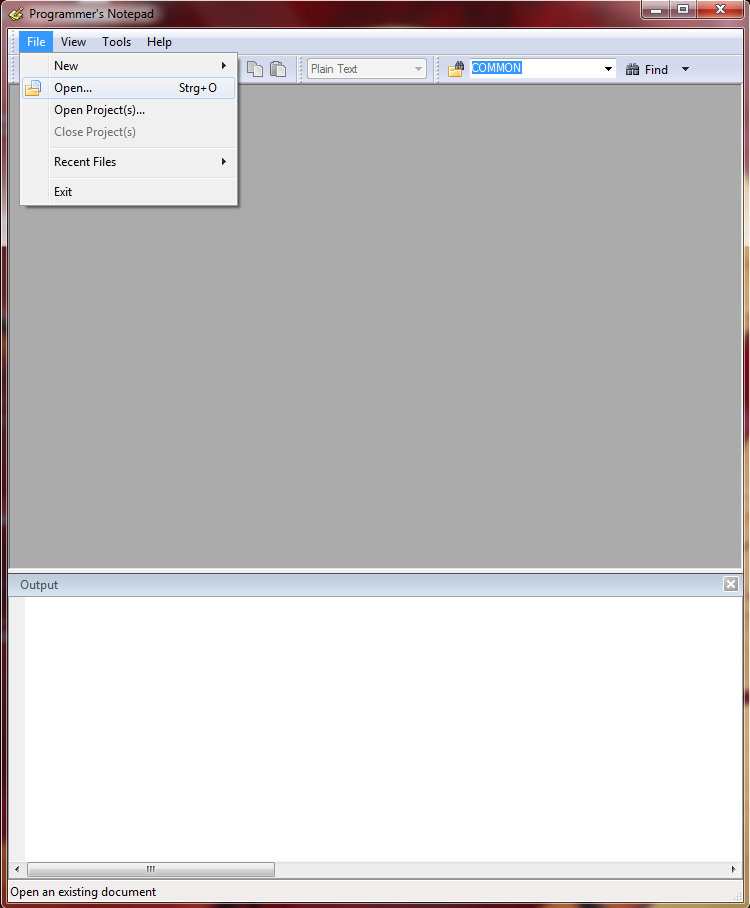
\includegraphics[width=9cm]{../PNG/Notepad_open.png}
    \caption{open Makefile}
  \end{subfigure}
  ~
  \begin{subfigure}[b]{9cm}
    \centering
    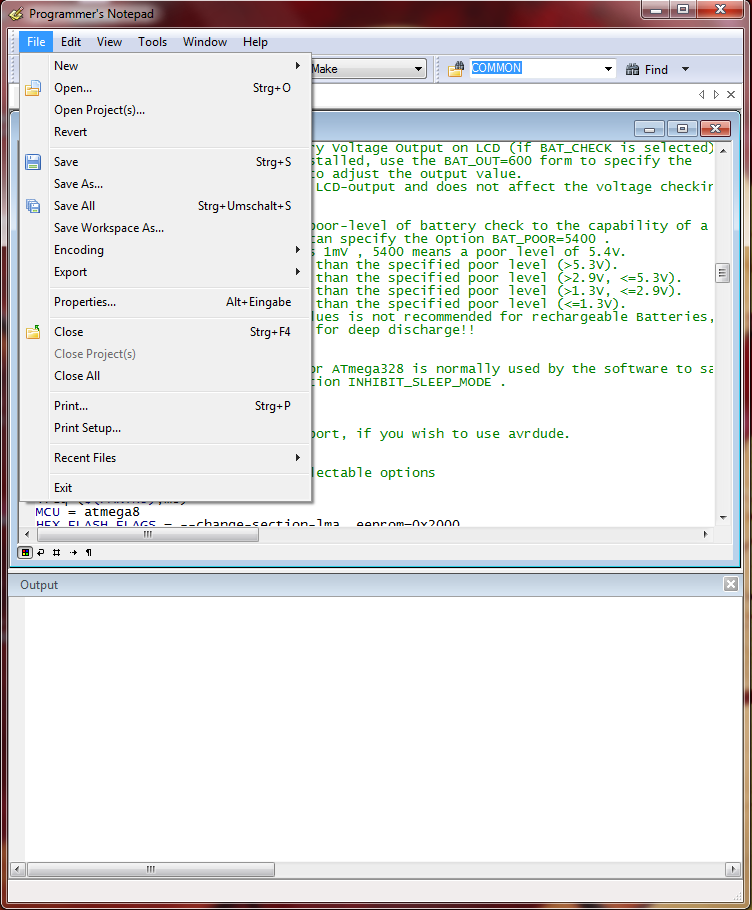
\includegraphics[width=9cm]{../PNG/Notepad_save.png}
    \caption{save Makefile}
  \end{subfigure}
  \caption{Using of the WinAVR user interface Programmer's Notepad}
  \label{fig:WinAVR1}
\end{figure}

The next figures \ref{fig:WinAVR2} show the Tools menu of the Programmer's Notepad
for compiling the program (Make All) and for programming the ATmega (Program) with avrdude.

\begin{figure}[H]
  \begin{subfigure}[b]{9cm}
    \centering
    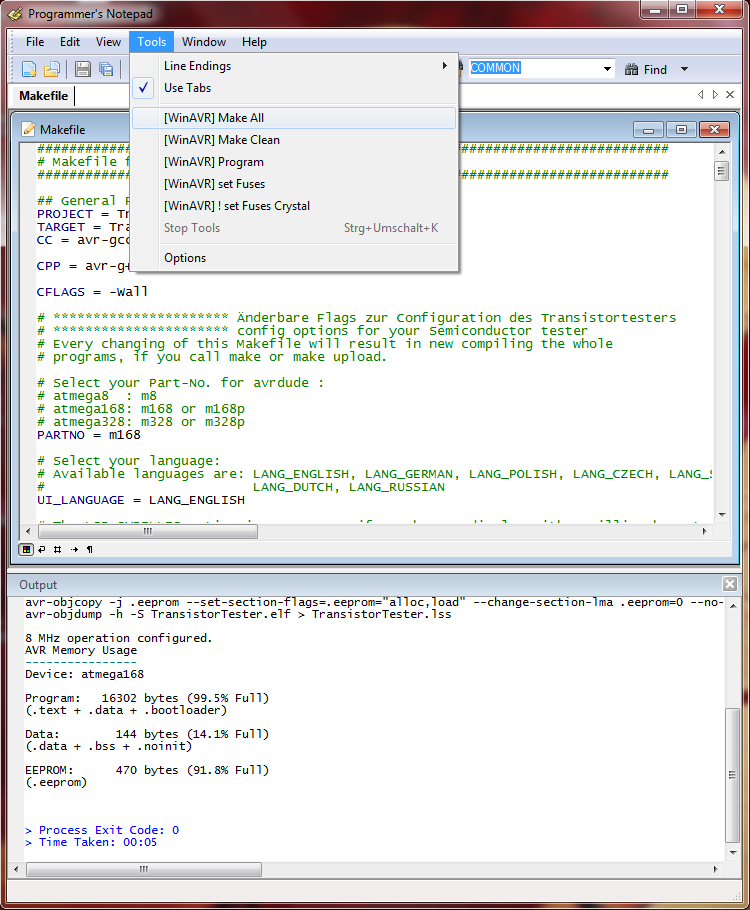
\includegraphics[width=9cm]{../PNG/Notepad_make.png}
    \caption{Build programming data (.hex/.eep)}
  \end{subfigure}
  ~
  \begin{subfigure}[b]{9cm}
    \centering
    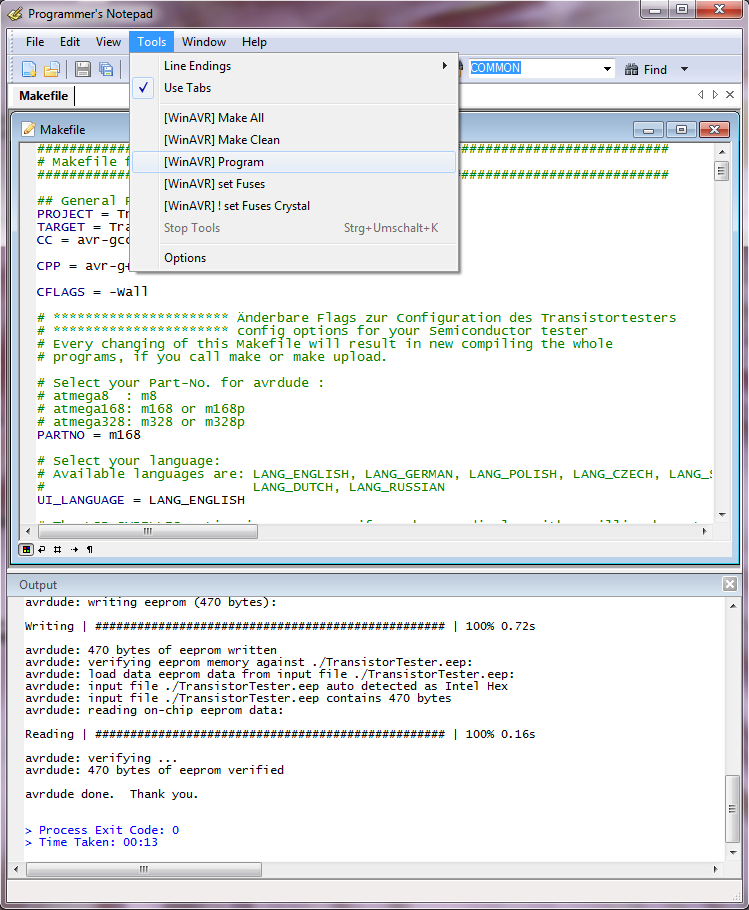
\includegraphics[width=9cm]{../PNG/Notepad_program.png}
    \caption{Programming the ATmega}
  \end{subfigure}
  \caption{Using of the WinAVR user interface Programmer's Notepad}
  \label{fig:WinAVR2}
\end{figure}



\section{Troubleshooting}
In most cases of problems you will miss the text output to the LCD-display.
At first you should check, if the LED was illuminated weak, if you release
the Test button. 
\begin{description}

\item[Power does not switch on.]
If the LED is without light and the VCC power has correct
5V voltage during holding the Test button, the microcontroller does not switch the power
correctly. The microcontroller should hold the power by switching the
PD6 output to 5V, which is usually done as one of the first actions.
If you hold the Test key pressed, the power is switched on anyway.
So you can check the value of VCC power and additionally the voltage value
of the PD6 output, if you hold the key pressed.
If VCC voltage has correct value (5V), but PD6 voltage is
below 4V, your microcontroller does not start the program. In this case
you should check if the microcontroller flash has been loaded with proper data for your
installed type and if ATmega is correctly configured with the fuses.
If your ATmega put the PD6 output to 5V and the power does not stay if you
release the Test key, it is more difficult to find the reason.
First you can shorten the LED and try again. If your Tester now starts,
your LED may be faulty or mounted with wrong polarity. If this is not
the reason, the current amplification factor of your T3 transistor (BC557C)
is insufficient. The current to the base of T3 is lower in the microcontroller
state as in the ``key pressed'' state.

\item[Nothing is readable on the LCD display]
Check the voltage at the contrast pin at the LCD display (pin 3). Adjust to
correct value specified in the data sheet of your display and optimize by viewing.
If you have a high temperature display type, you must provide a negative contrast voltage
for operation. In this case you can use the ICL~7660 device for generating
a negative voltage from positive 5V.

If there is no output readable on the LCD and the background light is on,
you should disconnect the power and check all four data plus the two control signal connections.
If all connection are well, the only reason I see is a uncorrect timing of
control signals. This can be caused by a slower LCD controller than expected by
the software or the ATmega software runs at wrong clock speed. Please check for which
clock speed your programming data was compiled  and if the fuses of the
ATmega are correct set to that speed. You find the clock parameter in the corresponding
Makefile.
If the tester is build without the switch off electronic, you can test with
a LED connected to the test pins, if the program operates normally.
If the LED flickers, the program operates well. The missing text on the
LCD must be caused by wrong connection or timing.


\item[Something but not all is readable on the LCD display]
Check if the .eep data are loaded to the EEprom memory of ATmega.
If all data are loaded correctly, you should check the clock speed of your
programming data (Makefile) and ATmega processor settings (fuses).

\item[Measurement is slow and Capacitors are measured about 8 times too small]
You run software compiled for 8MHz clock at real clock speed of 1MHz.
Please set the fuses of the ATmega correctly.

\item[Measurement has strangely values]
Check if your programmer is still connected to the ISP-plug.
The ISP interface should be disconnected for measuring.
Very often the reason of wrong measurements is the use of software compiled with
the AUTOSCALE\_ADC option and with the option NO\_REF\_CAP, but the capacitor
at the AREF pin has still a value of 100nF.
Wrong assembly of components or remaining soft solder flux can disturb the 
measurements too. Please check with the selftest function of your TransistorTester software
if possible. For the details see Chapter \ref{sec:selftest}.

Otherwise inspect your board visually and check the resistor values
with a ohmmeter. You can use the pins of the ATmega for this check, for example
to check the R1 you can measure between pin 23 and pin 14. Take a look at the
circuit diagram \ref{fig:ttester} for details. There is no need to
remove the microcontroller, only battery or power supply should be removed before.

\item[The Tester switch off the power after 2 seconds display time] 
This condition exists, if the external Pull-Up resistor at the PD7 input
is missing or the key button is keep pressed.
The software switch off the internal Pull-Up resistors to prevent a influence
to the measurement results. Therefore a external Pull-Up resistor (27k) is required.

\item[Der Tester shows only Vext=xx.xV in row 2]
This problem exists, if the Pull-Up resistor at the PD7 input
is missing or the key button is keep pressed.
Additionally the software is configured without the serial output (without option WITH\_UART) and
without the internal Pull-Up resistors (with option PULLUP\_DISABLE).
You should install the Pull-Up resistor at pin PD7.


\end{description}


\chapter{Bedienungshinweise}
\label{sec:manual}
\section{Der Meßbetrieb}
Die Bedienung des Transistortesters ist einfach.
Trotzdem sind einige Hinweise erforderlich.
Meistens sind an die drei Testports über Stecker-Leitungen mit Krokodilklemmen oder anderen Klemmen angeschlossen.
Es können auch Fassungen für Transistoren angeschlossen sein.
In jedem Fall können Sie Bauteile mit drei Anschlüssen mit den drei Testports in beliebiger Reihenfolge verbinden.
Bei zweipoligen Bauteilen können Sie die beiden Anschlüsse mit beliebigen Testports verbinden.
Normalerweise spielt die Polarität keine Rolle, auch Elektrolytkondensatoren können beliebig angeschlossen werden.
Die Messung der Kapazität wird aber so durchgeführt, dass der Minuspol am Testport mit der kleineren Nummer liegt.
Da die Messspannung aber zwischen 0,3 V und maximal 1,3 V liegt, spielt auch hier die Polarität keine wichtige Rolle.
Wenn das Bauteil angeschlossen ist, sollte es während der Messung nicht berührt werden. Legen Sie es auf einen
isolierenden Untergrund ab, wenn es nicht in einem Sockel steckt. Berühren Sie auch nicht die Isolation der Messkabel,
das Messergebnis kann beeinflusst werden.
Dann sollte der Starttaster gedrückt werden.
Nach einer Startmeldung erscheint nach circa zwei Sekunden das Messergebnis. Bei einer Kondensatormessung kann es
abhängig von der Kapazität auch deutlich länger dauern.

Was dann weiter geschieht, hängt von der Softwarekonfiguration des Testers ab.
\begin{description}
  \item[Einzelmessung] Wenn der Tester für Einzelmessung konfiguriert ist (POWER\_OFF Option),
 schaltet der Tester nach einer Anzeigezeit
von 28 Sekunden (konfigurierbar) wieder automatisch aus, um die Batterie zu schonen.
Während der Anzeigezeit kann aber auch vorzeitig eine neue Messung gestartet werden.
Nach der Abschaltung kann natürlich auch wieder eine
neue Messung gestartet werden, entweder mit dem gleichen Bauteil oder mit einem anderen Bauteil.
Wenn die Elektronik zum Abschalten fehlt, wird das letzte Meßergebnis weiter angezeigt.

  \item[Dauermessung] Einen Sonderfall stellt die Konfiguration ohne die automatische Abschaltfunktion dar.
Hierfür wird die POWER\_OFF Option in der Makefile nicht gesetzt.
Diese Konfiguration wird normalerweise nur ohne die Transistoren für die Abschaltung benutzt.
Es wird stattdessen ein externer Ein-/Aus-Schalter benötigt. Hierbei wiederholt der Tester die
Messungen solange, bis ausgeschaltet wird.

  \item[Serienmessung] In diesem Konfigurationsfall wird der Tester nicht nach einer Messung sondern erst nach einer konfigurierbaren
Zahl von Messungen abgeschaltet. Hierfür wird der POWER\_OFF Option in der Makefile eine Wiederholzahl (z.B. 5) zugewiesen.
Im Standardfall wird der Tester nach fünf Messungen ohne erkanntes Bauteil abgeschaltet.
Wird ein angeschlossenes Bauteil erkannt, wird erst bei der doppelten Anzahl, also zehn Messungen abgeschaltet.
Eine einzige Messung mit nicht erkanntem Bauteil setzt die Zählung für erkannte Bauteile auf Null zurück.
Ebenso setzt eine einzige Messung mit erkannten Bauteil die Zählung für die nicht erkannten Bauteile auf Null zurück.
Dies hat zur Folge, dass auch ohne Betätigung des Starttasters immer weiter gemessen werden kann,
 wenn Bauteile regelmässig gewechselt werden.
Ein Bauteilwechsel führt in der Regel durch die zwischenzeitlich leeren Klemmen zu einer Messung ohne erkanntes Bauteil.

Eine Besonderheit gibt es in diesem Betriebsmodus für die Anzeigezeit. Wenn beim Einschalten der Starttaster nur kurz
gedrückt wurde, beträgt die Anzeigezeit der Messergebnisse nur 5 Sekunden. Wenn der Starttaster bis zum Erscheinen der
ersten Meldung festgehalten wurde, beträgt die Anzeigezeit wie bei der Einzelmessung 28 Sekunden.
Ein vorzeitiger neuer Messbeginn ist aber während der Anzeigezeit durch erneutes Drücken des Starttasters möglich.

\end{description}

\section{Optionale Menüfunktionen für den ATmega328}
Wenn die Menü Funktion eingeschaltet ist, startet der Tester nach einem längeren Tastendruck (\textgreater~500ms) ein Auswahlmenü
für zusätzliche Funktionen.
Die wählbaren Funktionen erscheinen in Zeile~2 eines zweizeiligen Displays oder werden als gekennzeichnete
Funktion in Zeile 3 eines vierzeiligen Displays gezeigt. Dabei wird die vorige und nächste Funktion in Zeile 2 und 4 angezeigt.
Nach einer längeren Wartezeit ohne jegliche Bedienung kehrt das Programm zu der normalen Transistortester-Funktion zurück.
Durch kurzen Tastendruck kann zur nächsten Auswahl gewechselt werden.
Mit einem längeren Tastendruck startet die angezeigte Zusatzfunktion.
Nach Anzeige der letzten Funktion ,,Schalte aus'' wird wieder die erste Funktion angezeigt.\\

Wenn der Tester mit einem Drehimpulsgeber ausgerüstet ist, kann die Menü-Auswahl auch mit einem schnellen
Drehen des Encoders während der Anzeige einer vorausgegangenen Messung aufgerufen werden.
Die Menüfunktionen können mit einem langsamen Drehen des Encoders in beliebiger Richtung ausgewählt werden.
Die ausgewählte Menüfunktion kann aber nur mit einem längeren Tastendruck gestartet werden.
Innerhalb einer Menüfunktion können Parameter durch eine langsame Drehung des Encoders ausgewählt werden.
Eine schnelle Drehung des Encoders kehrt zur Menü-Auswahl zurück.

\begin{description}
 \item[Frequenz]
Die Zusatzfunktion ,,Frequenz'' (Frequenzmessung) benutzt als Eingang den PD4 Pin des ATmega, der auch an das LCD angeschlossen ist.
Es wird immer zunächst die Frequenz gemessen, bei Frequenzen unter \(25 kHz\) wird auch die mittlere Periode des Eingangssignals
bestimmt und daraus die Frequenz mit einer Auflösung von bis zu \(0.001 Hz\) berechnet.
Bei gesetzter POWER\_OFF Option in der Makefile wird die Dauer der Frequenzmessung auf 8~Minuten beschränkt.
Die Frequenzmessung wird durch Tastendruck beendet und in das Auswahlmenü zurückgekehrt.\\

 \item[f-Generator]
Bei der Zusatzfunktion ,,f-Generator'' (Frequenz Generator) können die Frequenzen durch einen Tastendruck 
 gewechselt werden.
Nachdem aus der Liste die letzte Frequenz gewählt wurde, wird als nächstes die erste Frequenz
 wieder ausgegeben (zyklische Wahl).
Bei gesetzter POWER\_OFF Option in der Makefile muß für den Frequenzwechsel die Taste länger gedrückt werden, da
durch einen kurzen Tastendruck (\textless~0.2~s) nur die Zeitüberwachung von 4~Minuten zurückgesetzt wird.
Die abgelaufene Zeit wird in Zeile 1 durch einen Punkt für jede abgelaufene 30 Sekunden angezeigt.
Durch einen regelmäßigen kurzen Tastendruck kann die vorzeitige Abschaltung der Frequenzerzeugung verhindert werden.
Ein längerer Tastendruck (\textgreater~0.8~s) kehrt wieder zur Auswahl der Funktionen zurück.\\

 \item[10-bit PWM]
Bei der Zusatzfunktion ,,10-bit PWM'' (Pulsweitenmodulation) wird eine feste Frequenz mit einstellbarer Pulsweite an Pin TP2 erzeugt.
Mit einem kurzen Tastendruck (\textless~0.5~s) wird die Pulsweite um \(1 \%\) erhöht, mit einem längeren Tastendruck um \(10 \%\).
Bei Überschreiten von \(99 \%\) werden \(100 \%\) vom erhöhten Wert abgezogen.
Bei gesetzter POWER\_OFF Option in der Makefile wird die Frequenzerzeugung nach 8 Minuten ohne Bedienung beendet.
Durch sehr langen Tastendruck (\textgreater~1.3~s) kann die Frequenzerzeugung auch beendet werden.\\

 \item[C+ESR@TP1:3]
Bei der Zusatzfunktion ,,C+ESR@TP1:3'' wird eine separate Kondensatormessung mit ESR-Messung an TP1 und TP3 gestartet.
Meßbar sind Kondensatoren mit mehr als \(2 \mu F\) bis zu \(50 mF\). Wegen der geringen Meßspannung von etwa 300mV sollte
in vielen Fällen die Messung in der Schaltung ohne vorherigen Ausbau möglich sein.
Bei gesetzter POWER\_OFF Option in der Makefile ist die Anzahl der Messungen auf 250 beschränkt,
kann aber sofort wieder gestartet werden.
Die Mess-Serie kann durch einen längeren Tastendruck  beendet werden.\\

 \item[Impulsdrehgeber]
Mit der Zusatzfunktion ,,Impulsdrehgeber'' kann ein Drehgeber untersucht werden.
Die drei Kontakte des Impulsdrehgebers müssen vor dem Start der Zusatzfunktion an die drei Testpins
 des Transistortesters angeschlossen werden.
Nach dem Start der Funktion muß der Drehknopf gedreht werden.
Dabei wird der gemeinsame Anschluß herausgefunden und angezeigt, ob jede Raststellung beide Kontake offen ('o')
oder beide Kontakte geschlossen ('C') hat.
Wenn beide Schalterstellungen an den Raststellungen vorkommen,
werden beide Zeichen alternierend angezeigt.\\

 \item[Selbsttest]
Mit der Zusatzfunktion ,,Selbsttest'' wird ein vollständiger Selbsttest mit Kalibration durchgeführt.
Dabei werden sowohl die Testfunktionen T1 bis T7 (wenn nicht verhindert mit der Option NO\_TEST\_T1\_T7) 
als auch die Kalibration mit dem externen Kondensator jedes Mal durchgeführt.\\

 \item[Spannung]
Die Zusatzfunktion ,,Spannung'' (Spannungsmessung) ist nur möglich, wenn die serielle Ausgabe deaktiviert wurde
oder der ATmega mindestens 32 Pinne hat (PLCC) und einer der zusätzlichen Pinne ADC6 oder ADC7 für die Messung benutzt wird.
Da am Port PC3 (oder ADC6/7) ein 10:1 Spannungsteiler vorgesehen ist, können Spannungen bis 50V gemessen werden.
Ein installierter DC-DC Wandler für die Zenerdioden-Messung wird durch Tastendruck eingeschaltet.
So können auch angeschlossene Zenerdioden gemessen werden.
Bei gesetzter POWER\_OFF Option in der Makefile und ohne Bedienung wird die Messung nach 4~Minuten beendet.
Die Messung kann aber durch einen besonders langen Tastendruck (\textgreater~4~Sekunden) vorher beendet werden.\\

\item[Kontrast] 
Diese Funktion kann den Kontrast für ein graphisches Display mit st7565 Kontroller einstellen.
Der Einstellwert kann mit einem sehr kurzen Tastendruck oder einer Linksdrehung des Impulsdrehgebers verringert werden.
Ein längerer Tastendruck oder eine Rechtsdrehung des Impulsdrehgebers vergrößert den Einstellwert.
Die Funktion wird beendet und der eingestellte Wert wird permanent in den EEprom Speicher geschrieben, 
wenn die Taste noch länger gedrückt wird.

 \item[Zeige Daten]
Die Funktion ,,Zeige Daten'' zeigt neben der Software-Versionsnummer die Daten des Abgleichs an.
Dies sind die Nullwiderstände R0 von Pin 1:3, 2:3 und 1:2 .
Außerdem werden die Ausgangswiderstände der Ports zur 5V Seite (RiHi) und 
zur 0V Seite (RiLo) angezeigt.
Die Nullkapazitätswerte (C0) werden ebenfalls in allen Pinkombibationen angezeigt (1:3, 2:3, 1:2 und 3:1, 3:2 2:1).
Zuletzt werden auch die Spannungskorrekturen für die Komparatorspannung (REF\_C) und für die Referenzspannung (REF\_R) angezeigt.
Jede Seite wird 15 Sekunden angezeigt.
Es kann aber auch durch Tastendruck oder einer Rechtsdrehung des Impulsdrehgebers
zur nächsten Seite geblättert werden.
Mit einer Linksdrehung des Impulsdrehgebers kann die Ausgabe wiederholt werden oder zur vorigen Seite zurückgeblättert werden.

 \item[Schalte aus]
Mit der Zusatzfunktion ,,Schalte aus'' kann der Transistortester abgeschaltet werden.\\

 \item[Transistor]
Natürlich kann mit der Funktion ,,Transistor'' (Transistor Tester) wieder zu der normalen Transistortester Funktion
zurückgekehrt werden.

\end{description}

Bei gesetzter POWER\_OFF Option in der Makefile sind alle Zusatzfunktionen zeitbeschränkt, damit die Batterie nicht verbraucht wird.

\section{Selbsttest und Kalibration}

Wenn die Software mit der Selbsttestfunktion konfiguriert ist, kann der Selbsttest durch einen Kurzschluss aller drei
Testports und drücken der Starttaste eingeleitet werden.
Für den Start des Selbsttests muß die Starttaste innerhalb von 2 Sekunden noch einmal gedrückt werden,
sonst wird mit einer normalen Messung fortgefahren.
Beim Selbsttest werden die im Selbsttest-Kapitel \ref{sec:selftest} beschriebenen Tests ausgeführt.
Wenn der Tester mit einer Menüfunktion (Option WITH\_MENU) konfiguriert ist, 
wird der vollständige Selbsttest mit den Tests T1 bis T7 nur bei dem ,,Selbsttest'' ausgeführt, 
der als Menüfunktion ausgewählt werden kann.
Außerdem wird beim Aufruf über die Menü Funktion der Abgleich mit dem externen Kondensator jedesmal durchgeführt,
sonst nur für den ersten Aufruf.
Damit kann der durch die kurgeschlossenen Testports automatisch gestartete Abgleich schneller durchgeführt werden. 
Die viermalige Testwiederholung bei T1 bis T7 kann vermieden werden, wenn der Starttaster gedrückt gehalten wird.
So kann man uninteressante Tests schnell beenden und
sich durch Loslassen des Starttasters interessante Tests viermal wiederholen lassen.
Der Test 4 läuft nur automatisch weiter, wenn die Verbindung zwischen den Testports gelöst wird.

Wenn die Funktion AUTO\_CAL in der Makefile gewählt ist, wird beim Selbsttest
eine Kalibration der Nullwertes für die Kondensatormessung durchgeführt.
Für die Kalibration des Nullwertes für die Kondensatormessung ist wichtig, 
daß die Verbindung zwischen den Testpins (Kurzschluß) während des Tests 4 wieder gelöst wird!
Sie sollten während der Kalibration (nach dem Test 6) weder die Testports noch angeschlossene Kabel berühren.
Die Ausrüstung sollte aber die gleiche sein, die später zum Messen verwendet wird.
Anderenfalls wird der Nullwert der Kondensatormessung nicht richtig bestimmt.
Die Kalibration des Innenwiderstandes der Port-Ausgänge wird mit dieser Option vor jeder
Messung durchgeführt.

Für den letzten Teil der Kalibration ist der Anschluß eines Kondensators 
mit einer beliebiger Kapazität zwischen \(100 nF\) und \(20 \mu F\) an Pin~1 und Pin~3 erforderlich.
Dazu wird in Zeile 1 ein Kondensatorsymbol zwischen den Pinnummern 1 und 3 angezeigt, gefolgt von dem Text ,, \textgreater100nF''.
Sie sollten den Kondensator erst nach dieser Ausgabe anschließen.
Mit diesem Kondensator wird die Offset Spannung des analogen Komparators kompensiert,
um genauere Kapazitätswerte ermitteln zu können.
Die Verstärkung für ADC Messungen mit der internen Referenz-Spannung wird ebenfalls mit diesem Kondensator abgeglichen, um
bessere Widerstands-Messergebnisse mit der AUTOSCALE\_ADC Option zu erreichen.
Wenn die Menü Funktion beim Tester ausgewählt wurde (Option WITH\_MENU) und der Selbsttest
nicht als Menü Funktion gestarte wurde, wird der Abgleich mit dem externen Kondensator nur bei
der ersten Kalibration durchgeführt.
Die Kalibration mit dem externen Kondensator kann nur wiederholt werden, wenn der Selbsttest
als Menü Funktion ausgewählt wird.

Der Nullwert für die ESR-Messung wird als Option ESR\_ZERO in der Makefile vorbesetzt.
Mit jedem Selbsttest wird der ESR Nullwert für alle drei Pinkombinationen neu bestimmt.
Das Verfahren der ESR-Messung wird auch für Widerstände mit Werten unter \(10 \Omega\) benutzt um
hier eine Auflösung von \(0.01 \Omega\) zu erreichen.

\section{Besondere Benutzungshinweise}
Normalerweise wird beim Start des Testers die Batteriespannung angezeigt. Wenn die Spannung eine Grenze unterschreitet, 
wird eine Warnung hinter der Batteriespannung ausgegeben. Wenn Sie eine aufladbare 9V Batterie benutzen, sollten Sie
den Akku möglichst bald austauschen oder nachladen.
Wenn Sie eine Version mit eingebauter 2.5V Präzisionsreferenz besitzen, wird beim Start für eine Sekunde die
gemessene Betriebsspannung in der Zeile 2 mit ,,VCC=x.xxV'' angezeigt.

Es kann nicht oft genug erwähnt werden, daß Kondensatoren vor dem Messen entladen sein müssen.
Sonst kann der Tester schon defekt sein, bevor der Startknopf gedrückt ist.
Wenn man versucht, Bauelemente im eingebauten Zustand zu messen, sollte das Gerät immer von
der Stromquelle getrennt sein. Außerdem sollte man sicher sein, daß keine Restspannung mehr
im Gerät vorhanden ist. Alle Geräte haben Kondensatoren verbaut!

Beim Messen kleiner Widerstandswerte muß man besonders auf die Übergangswiderstände achten.
Es spielt die Qualität und der Zustand von Steckverbindern eine große Rolle, genau so wie die
Widerstandwerte von Meßkabeln. Dasselbe gilt auch für die Messung des ESR Wertes von Kondensatoren.
Bei schlechten Anschlußkabeln mit Krokodilklemmen wird so aus einem ESR von \(0.02 \Omega\) leicht
ein Wert von \(0.61 \Omega\).

An die Genauigkeit der Meßwerte sollte man keine übertriebenen Erwartungen haben, dies gilt besonders
für die ESR Messung und die Induktivitätsmessung.
Die Ergebnisse meiner Meßreihen kann man im Kapitel \ref{sec:measurement} finden.


\section{Problemfälle}
Bei den Meßergebnissen sollten Sie immer im Gedächtnis behalten, daß die Schaltung des Transistortesters für
Kleinsignal Bauelemente ausgelegt ist. Normalerweise beträgt der maximale Meßstrom etwa 6 mA.
Leistungshalbleiter machen oft wegen hoher Reststöme Probleme bei der Erkennung oder beim Messen der
Sperrschicht-Kapazität.
Bei Thyristoren und Triacs werden oft die Zündströme oder die Halteströme nicht erreicht. Deswegen kann es
vorkommen, daß ein Thyristor als NPN Transistor oder Diode erkannt wird. Ebenso ist es möglich, daß ein 
Thyristor oder Triac gar nicht erkannt wird.

Probleme bei der Erkennung machen auch Halbleiter mit integrierten Widerständen.
So wird die Basis - Emitter Diode eines BU508D Transistors wegen eines parallel geschalteten internen
\(42 \Omega\) Widerstandes nicht erkannt.
Folglich kann auch die Transistorfunktion nicht geprüft werden.
Probleme bei der Erkennung machen oft auch Darlington Transistoren höherer Leistung. Hier sind auch
oft Basis - Emitter Widerstände verbaut, welche die Erkennung wegen der hier verwendeten kleinen Meßströme erschweren.

\section{Messung von PNP und NPN Transistoren}
Normalerweise werden die drei Anschlüsse des Transistors in beliebiger Reihenfolge an die Meßeingänge des
Transistortesters angeschlossen.
Nach dem Drücken des Starttasters meldet der Tester in der Zeile 1 den Typ (NPN oder PNP), 
eine eventuell vorhandene Schutzdiode der Kollektor - Emitter Strecke und
die Anschlußbelegung. Das Diodensymbol wird  polungsrichtig angezeigt.
In der Zeile 2 wird der Stromverstärkungsfaktor (B=...) und die Basis - Emitter Schwellspannung ausgegeben.
Hierbei sollte man wissen, daß der Tester den Stromverstärkungsfaktor in zwei Schaltungsvarianten 
ermittelt, der Emitterschaltung und der Kollektorschaltung (Emitterfolger).

Bei der Emitterschaltung hat der Tester nur zwei Möglichkeiten, den Basisstrom einzustellen:
\begin{enumerate}
\item Mit dem \(680 \Omega\) Widerstand ergibt sich ein Basisstrom von etwa 6.1mA . Das ist für einen
Kleinsignaltransistor mit hohem Verstärkungsfaktor meist zu viel, weil die Basis gesättigt ist.
Da der Kollektorstrom ebenfalls mit einem \(680 \Omega\) Widerstand gemessen wird, kann der Kollektorstrom
den um den Verstärkungsfaktor höheren Strom gar nicht erreichen. Die Softwareversion vom Markus F. hat
in diesem Zustand die Basis - Emitter Spannung gemessen (Uf=...).\\
\item Mit dem \(470 k\Omega\) Widerstand] ergibt sich ein Basisstrom von nur \(9.2 \mu A\) .
Das ist für einen Leistungstransistor mit geringem Verstärkungsfaktor sehr wenig.
Die Softwareversion von Markus F. hat in diesem Zustand den Stromverstärkungsfaktor bestimmt (hFE=...).\\
\end{enumerate}

Die Software des Testers bestimmt die Stromverstärkung jetzt auch in der Kollektorschaltung.
Ausgegeben wird der höhere Wert der beiden Mess-Methoden.
Die Kollektorschaltung hat den Vorteil, daß sich durch die Stromgegenkopplung der Basisstrom abhängig vom
Verstärkungsfaktor reduziert. Dadurch kann für Leistungstransistoren mit dem \(680 \Omega\) und für Darlington Transistoren
mit dem \(470 k\Omega\) Widerstand meist ein günstigerer Meßstrom ergeben.
Die ausgegebene Basis Emitter Schwellspannung Uf ist jetzt die Spannung,
die bei der Bestimmung des Stromverstärkungsfaktors gemessen wurde.
Wenn man trotzdem eine Basis - Emitter Schwellspannung bei circa 6 mA ermitteln möchte, muß man den Kollektor
vom Tester trennen und noch einmal messen.
Dann wird die Schwellspannung bei etwa 6mA ausgegeben und die Kapazität der Diode in Sperr-Richtung ermittelt.
Natürlich kann so auch die Basis - Kollektor Diode gemessen werden.

Bei Germanium Transistoren wird meistens ein Kolleḱtor-Emitter Reststrom \(I_{CE0}\) mit stromloser Basis oder
ein Kollektor-Emitter Reststrom \(I_{CES}\) mit Basis auf Emitterpotential gemessen.
In diesem Fall werden in Zeile 2 für ATmega328 für 5 Sekunden oder bis zum Tastendruck die Restströme
vor der Stromverstärkung ausgegeben.
Durch Kühlen kann der Reststrom bei Germanium Transistoren erheblich gesenkt werden. 

\section{Messung von JFET und D-MOS Transistoren}
Wegen des symmetrischen Aufbaus von JFET Transistoren kann Source und Drain nicht unterschieden werden.
Normalerweise wird bei JFET als eine Kenngröße der Strom bei kurzgeschlossenem Gate - Source angegeben.
Dieser Strom ist aber oft höher als der, der sich bei der Meßschaltung mit dem \(680 \Omega\) Widerstand erreichen läßt.
Deswegen wird der \(680 \Omega\) Widerstand an den Source Anschluß geschaltet. Dadurch erhält das Gate
stromabhängig eine negative Vorspannung. Als Kenngröße wird sowohl der ermittelte Strom als auch die
Gate - Source Spannung ausgegeben. 
Damit können verschiedene Typen unterschieden werden.
Für D-MOS Transistoren (Verarmungs-Typ) wird das gleiche Meßverfahren verwendet.

Für Anreicherungs MOS Transistoren (P-E-MOS oder N-E-MOS) sollte man wissen, daß die Bestimmung der Gate Schwellspannung (Vth)
bei kleiner Gate  Kapazität schwierig wird. Hier können mit dem Tester genauere Spannungswerte ermittelt werden, wenn ein
Kondensator mit einigen nF parallel zum Gate / Source angeschlossen wird.
Die Schwellspannung wird bei Drain Strömen von etwa 3.6mA für P-E-MOS und bei etwa 4mA für N-E-MOS bestimmt.


\chapter{Konfigurieren des TransistorTesters}
\label{sec:config}
Die ganze Software des TransistorTesters ist im Quellcode verfügbar.
Die Übersetzung der Module wird mit einer Makefile gesteuert. Die Entwicklung wurde
auf einen Ubuntu Linux Betriebssystem mit den GNU-Werkzeugen (GNU toolchain, gcc version 4.5.3) durchgeführt.
Es sollte möglich sein, ohne Schwierigkeiten andere Linux-Betriebssysteme zu benutzen.
Um die übersetzen Daten in den Flash-Speicher oder den EEprom-Speicher zu laden, wird das
Programm avrdude \cite{avrdude} (Version 5.11svn) von der Makefile benutzt, wenn man ,,make upload'' aufruft.
Das Programm avrdude ist für Linux und Windows verfügbar.
Der GNU C-Kompiler wird auch von der AVR-studio-Software unter Windows oder von
der WinAVR \cite{winavr1},\cite{winavr2} Software benutzt.
Sie können die Programmdaten (.hex und .eep) auch mit anderen Programmen in den ATmega laden,
aber nur meine Makefile Version stellt sicher, dass die richtigen Daten in den gewählten Prozessor gelangen.
Avrdude lädt Daten nur in den ATmega, wenn die Signaturbytes des angeschlossenen ATmega gleich mit dem ausgewählten sind.
Wenn Sie die Makefile ändern, wird die Software komplett neu übersetzt, wenn man ,,make'' oder
,,make upload'' aufruft.
Die Software, die für einen ATmega8 übersetzt wurde, läuft nicht auf einem ATmega168.
Die Software, die für einen ATmega328 übersetzt wurde, läuft nicht auf einem ATmega168.
Eine Ausnahme bildet Software, die für einen ATmega168 übersetzt wurde. Diese Programmdateien
sind auch für einen ATmega328 brauchbar.
Sind Sie vorsichtig, wenn Sie nicht das mitgelieferte Makefile benutzen.

Mit den entsprechenden Optionen ist die Software auch auf dem unveränderten Hardware-Entwurf von
Markus F. lauffähig (PARTNO=m8 , {\bf keine} NO\_AREF\_CAP und {\bf keine} PULLUP\_DISABLE Option).
Die Taktrate kann mit den fuses auch auf 8MHz gestellt werden, dazu ist kein Quarz erforderlich!


Die folgenden Optionen der Makefile sind verfügbar, um die Software für den Tester zu konfigurieren:

\begin{description}
  \item[PARTNO] beschreibt den Ziel-Prozessor:\\
         m8 = ATmega8\\
         m168 or m168p = ATmega168\\
         m328 or m328p = ATmega328\\
    Beispiel: PARTNO = m168
  \item[UI\_LANGUAGE] gibt die Sprache für den Tester an:\\
    LANG\_ENGLISH, LANG\_GERMAN, LANG\_POLISH, LANG\_CZECH, LANG\_SLOVAK, LANG\_SLOVENE, LANG\_DUTCH, LANG\_BRASIL,
 LANG\_RUSSIAN, LANG\_UKRAINIAN and LANG\_LITHUANIAN sind derzeit verfügbar.
 Für die russische und ukrainische Sprache ist ein LCD mit kyrillischem Zeichensatz erforderlich.\\
    Beispiel: UI\_LANGUAGE = LANG\_ENGLISH
  \item[LCD\_CYRILLIC] wird nur gebraucht, wenn man ein LCD-Display mit kyrillischem Zeichensatz benutzt.
Die Zeichen \(\mu\) und \(\Omega\) sind im kyrillischen Zeichensatz nicht enthalten.
Wenn Sie diese Option angeben, werden beide Zeichen von der Software in das LCD geladen.\\
Beispiel: CFLAGS += -DLCD\_CYRILLIC
  \item[LCD\_DOGM] muß angegeben werden, wenn ein LCD mit ST7036 Controller (Typ DOG-M) zur Anzeige verwendet wird.
Der LCD-Kontrast wird dann mit Software-Befehlen eingestellt.
Beispiel: CFLAGS += -DLCD\_DOGM
  \item[FOUR\_LINE\_LCD] kann bei einem 4x20 Zeichen Display verwendet werden, um den Platz auf dem Display
besser auszunutzen. Zusätzliche Parameter, welche sonst nur kurz in Zeile 2 angezeigt werden, werden dann in
den Zeilen 3 und 4 angezeigt.\\
Beispiel: CFLAGS += -DFOUR\_LINE\_LCD
  \item[WITH\_LCD\_ST7665] Diese Option muß verwendet werden, wenn ein 128x64 Pixel LCD mit serieller
Schnittstelle angeschlossen ist. Für diesen Display Typ müssen weitere Optionen gesetzt werden, die im Folgenden
beschrieben werden.\\
Beispiel: WITH\_LCD\_ST7565 = 1 
  \item[LCD\_ST7565\_RESISTOR\_RATIO] Mit dieser Option wird das Widerstands Teilerverhältnis für den
Spannungsregler des ST7565 controller eingestellt. Brauchbare Werte liegen im allgemeinen zwischen 4 und 7.
Einstellbar sind Werte zwischen 0 und 7.\\
Beispiel: LCD\_ST7564\_RESISTOR\_RATIO = 4
  \item[LCD\_ST7565\_H\_FLIP] Mit dieser Option kann die Anzeige horizontal umgedreht werden.\\
Beispiel: LCD\_ST7565\_H\_FLIP = 1
  \item[LCD\_ST7565\_H\_OFFSET] Diese Option kann den für die Ausgabe benutzten Speicher an das Anzeigefenster des
 Displays anpassen. Der Kontroller benutzt mehr horizontale Pixel (132) als angezeigt (128) werden.
 Je nach Lage des Anzeigefenster muß der Offset bei gedrehter oder normaler horizontaler Anzeigerichtung
 berücksichtigt werden.\\
Beispiel: LCD\_ST7565\_H\_OFFSET = 4
  \item[LCD\_ST7565\_V\_FLIP] Mit dieser Option kann die Anzeige vertikal umgedreht werden.\\
Beispiel: LCD\_ST7565\_V\_FLIP = 1
  \item[FONT\_8X16] You must select one font size for the ST7565 controller.
Selectable are FONT\_6X8, FONT\_8X8, FONT\_8X12, FONT\_8X16 and FONT\_16X16.
Font size 8X16 is the most efficient use of graphics space for a 128x64 pixel LCD.\\
example: FONT\_8X16
  \item[FONT\_8X16] Für den ST7565 controller sollte ein Fonts ausgewählt werden.
Auswählbar  sind FONT\_6X8, FONT\_8X8, FONT\_8X12, FONT\_8X14 und FONT\_16X16.
Derzeit wird nur der 6x8 und der 8x16 Font vollständig unterstützt.
Die Font Größe 8X16 ist die effizienteste Wahl für das graphische 128x64 LCD.\\
Beispiel: FONT\_8X16
  \item[STRIP\_GRID\_BOARD] Diese Option passt die Software an eine andere Pinbelegung von Port~D für Streifenleiterplatinen an.
Die Einzelheiten findet man im Hardwarekapitel \ref{sec:hardware}.
  \item[WITH\_MENU] aktiviert eine Menü Funktion für einen ATmega328.  Man kann einige Zusatzfunktionen über ein
Auswahlmenü benutzen, welches man über einen langen Tastendruck (\textgreater~0.5~s) erreichen kann.
Wenn die Menüfunktion eingeschaltet ist, wird beim automatischen Selbsttest Start mit kurzgeschlossenen Testpins
 nur der Kalibrationsteil des Selbsttests ausgeführt.
Die Tests T1-T7 werden nur beim Selbsttest ausgeführt, der als Menüfunktion ausgewählt werden kann.\\
Beispiel: CFLAGS += -DWITH\_MENU
  \item[WITH\_ROTARY\_SWITCH] Die Menü Funktion kann leicher bedient werden, wenn ein Impulsdrehgeber als Erweiterung
benutzt wird.
Für die Details der notwendigen Erweiterung sehen Sie bitte die Beschreibung~\ref{fig:RotExt} in dem Hardware Kapitel.
Wenn der Impulsdrehgeber die gleiche Anzahl von Raststellungen wie Impulse für jede Umdrehung hat,
muß die Option WITH\_ROTARY\_SWITCH auf 2 gesetzt werden.
Wenn der Impulsdrehgeber doppelt so viele Raststellungen hat, muß die Option WITH\_ROTARY\_SWITCH auf 1 gesetzt werden.
Das Setzen der Optione \_WITH\_ROTARY\_SWITCH auf 5 wählt die höchste Auflösung für den Impulsdrehgeber.
Jeder Zyklus der beiden Schalter-Zustände wird als 4 gezählt. Normalerweise ist diese Einstellung nur für
Impulsdrehgeber ohne Raststellung sinnvoll.
Ein Setzen der Option WITH\_ROTARY\_SWITCH auf 4 ist notwendig für die korrekte Behandlung von zwei separaten
Rauf (Up) und Runter (Down) Tastern, die anstelle der beiden Schalter eines Impulsdrehgebers eingebaut sind.
Verwenden Sie nicht die Einstellung 4 mit normalen Impulsdrehgebern!\\
Beispiel: CFLAGS += -DWITH\_ROTARY\_ENCODER=1
  \item[CHANGE\_ROTARY\_DIRECTION] Man kann die erkannte Drehrichtung des Impulsdrehgebers durch Vertauschen
der beiden Schalter-Signale oder durch Setzen der Option CHANG\_ROTARY\_DIRECTION ändern.
Beispiel: CFLAGS += -DCHANGE\_ROTARY\_DIRECTION
 \item[WITH\_SELFTEST] Wenn Sie diese Option angeben, baut die Software eine Selbsttest-Funktion ein, die gestartet wird
wenn Sie alle drei Prüfspitzen verbinden und eine Messung starten.\\
Beispiel: CFLAGS += -DWITH\_SELFTEST
  \item[NO\_COMMON\_COLLECTOR\_HFE] verhindert die hFE Messung von Transistoren in der Kollektorschaltung.
So können Sie Speicher sparen, um die erweiterten Selbsttest Routinen T1 bis T7 für den ATmega168 Prozessor zu ermöglichen.
Standardmäßig sind beide Schaltungen für die hFE Messung eingeschaltet,
aber da ist kein Platz im Programmspeicher des ATmega168 für die erweiterten Selbsttests.\\
Beispiel: CFLAGS += -DNO\_COMMON\_COLLECTOR\_HFE
  \item[NO\_COMMON\_EMITTER\_HFE] schaltet die hFE Messung von Transistoren in Emitterschaltung ab.
So können Sie Speicher sparen, um die erweiterten Selbsttest Routinen T1 bis T7 für den ATmega168 Prozessor zu ermöglichen.
Standardmäßig sind beide Schaltungen für die hFE Messung eingeschaltet,
aber dann ist kein Platz im Programmspeicher des ATmega168 für die erweiterten Selbsttests.\\
Beispiel: CFLAGS += -DNO\_COMMON\_EMITTER\_HFE
  \item[NO\_TEST\_T1\_T7] Diese Option verhindert die Ausführung der Selbsttest Teile T1 bis T7.
Diese Tests sind nützlich um Fehler in der Schaltung wie falsche Meßwiderstände oder Isolationsprobleme zu finden.
Wenn Ihre Schaltung fehlerfrei ist, können Sie die Selbsttest Teile T1 bis T7 durch das Setzen dieser Option weglassen, um eine
schnellere Kalibration zu erreichen.
Bei eingeschalteter Menüfunktion werden die Selbsttest Teile T1 bis T7 nur bei Aufruf der Menüfunktion ,,Selbsttest'' ausgeführt.
Der ATmega168 Prozessor benutzt die Selbsttest Teile T1 bis T7 nicht, wenn beide Meßmethoden für die hFE Bestimmung benutzt werden.\\
Beispiel: CFLAGS += -DNO\_TEST\_T1\_T7
  \item[AUTO\_CAL] Der Nullabgleich für die Kondensatormessung wird beim
Selbsttest zusätzlich ins EEprom geschrieben und ist damit für die weiteren Messungen abgeglichen.
Wenn nach dem Nullabgleich der Kondensatormessung ein Kondensator mit einer Kapazität zwischen \(100 nF\) und \(20 \mu F\) an Pin~1 und Pin~3 
angeschlossen wird, wird auch der Offset des analogen Komparators und die Skalierung für die AUTOSCALE\_ADC
Umschaltung auf die interne Spannungsreferenz ermittelt und ins EEprom geschrieben.
Die Port-Ausgangswiderstände werden zu Beginn jeder Messung neu bestimmt. \\
Beispiel: CFLAGS += -DAUTO\_CAL
  \item[FREQUENCY\_50HZ] Zum Ende des Selbsttests wird bis zu einer Minute lang ein 50 Hz Signal auf Port 2 und Port 3 erzeugt.\\
Beispiel: CFLAGS += -DFREQUENCY\_50HZ
  \item[CAP\_EMPTY\_LEVEL] Diese Option legt die Spannung (mV) für einen entladenen Kondensator fest.
Der Wert kann höher als 3mV gesetzt werden, wenn die Entladung nicht zum Ende kommt. In diesen Fall meldet der Tester nach längerer Zeit ,,Cell!''.\\
Beispiel: CFLAGS += -DCAP\_EMPTY\_LEVEL=3
  \item[WITH\_AUTO\_REF] Mit dieser Option wird die Referenzspannung gemessen, um den aktuellen Faktor für die Kapazitätsmessung 
von kleineren Kapazitäten (unter \(40\mu F\)) zu ermitteln.\\
Beispiel: CFLAGS += -DWITH\_AUTO\_REF
  \item[REF\_C\_KORR] gibt einen Offset für die gelesene Referenz-Spannung in mV-Einheiten an.
Das kann benutzt werden, um die Kapazitätsmessung kleiner Kondensatoren abzugleichen.
Wenn zusätzlich die AUTO\_CAL Option gewählt wurde, ist diese Angabe nur ein zusätzlicher Offset für
den gefundenen Komparator-Offset.
Ein Wert von 10 ergibt etwa 1~Prozent kleinere Messergebnisse.\\
Beispiel: CFLAGS += -DREF\_C\_KORR=14
  \item[REF\_L\_KORR] gibt einen zusätzlichen Offset für die Referenz-Spannung für die Induktivitätsmessung
in mV-Einheiten an. Der REF\_C\_KORR Offset beziehungsweise der gefundene Offset bei der Kalibration
wird bei der Induktivitätsmessung ebenfalls berücksichtigt.
Der REF\_L\_KORR Wert wird für die Messungen ohne \(680 \Omega\) Widerstand subtrahiert, bei Messungen mit einem
\(680 \Omega\) Widerstand wird der Wert addiert.\\
Beispiel: CFLAGS += -DREF\_L\_KORR=40
  \item[C\_H\_KORR] gibt eine Korrektur der Messergebnisse für grosse Kondensatoren an.
Eine Eingabe von 10 führt zu 1~Prozent kleineren Messergebnissen.\\
Beispiel: CFLAGS += -DC\_H\_KORR=10
  \item[WITH\_UART] benutzt den Pin PC3 zur Ausgabe der seriellen Texte (V24). Wenn die Option nicht
benutzt wird, kann der PC3 Pin zum Anschluß einer externen Spannung mit einem 10:1 Widerstandsteiler benutzt
werden. Damit können beispielsweise Zenerdioden mit höherer Durchbruchspannung getestet werden.
Diese Messung wird so lange mit etwa 3 Messungen pro Sekunde wiederholt, solange der Starttaster gedrückt bleibt.\\
Beispiel: CFLAGS += -DWITH\_UART
  \item[TQFP\_ADC6] Die Option TQFP\_ADC6 benutzt anstelle des PC3 Pins (ADC3) den zusätzlichen ADC-Eingang ADC6
des ATmegas im TQFP Gehäuse oder QFN Gehäuse.
Dadurch kann dieser Eingang unabhängig von der seriellen Ausgabe auf dem PC3 Pin genutzt werden. Dieser Pin wird
dann für die Zenerdioden Messung und für die Messung einer externen Spannung über den Dialog des ATmega328 genutzt.\\
Beispiel: CFLAGS += -DTQFP\_ADC6
  \item[TQFP\_ADC7] Die Option TQFP\_ADC7 benutzt anstelle des PC3 Pins (ADC3) den zusätzlichen ADC-Eingang ADC7
des ATmegas im TQFP Gehäuse und QFN Gehäuse.
Dadurch kann dieser Pin unabhängig von der seriellen Ausgabe auf den PC3 Pin genutzt werden. Wenn diese Option 
ohne die Option TQFP\_ADC6 genutzt wird, erfolgt sowohl die Zenerdioden Messung als auch die Messung einer externen
Spannung über den Dialog des ATmega328 genutzt. Wenn die Option zusätzlich zur TQFP\_ADC6 Option gesetzt wird,
erfolgt die Zenerdioden Messung mit dem ADC6 Pin und bei der über den Dialog wählbaren Spannungsmessung werden
beide Eingänge gemessen. Beide Pinne sollten dann an einen 10:1 Spannungsteiler angeschlossen sein.\\
Beispiel: CFLAGS += -DTQFP\_ADC7
  \item[WITH\_VEXT] ermöglicht die Messung einer externen Spannung über einen 10:1 Spannungsteiler.
Für den ATmega168 oder ATmega328 wird normalerweise der PC3 Pin benutzt, wenn keine Option TQFP\_ADC6 oder
TQFP\_ADC7 gesetzt ist. Dann ist diese Option aber nur möglich, wenn die WITH\_UART Option nicht gesetzt ist.\\
Beispiel: CFLAGS += -DWITH\_VEXT 
  \item[AUTOSCALE\_ADC] schaltet die automatische Bereichswahl des ADC (entweder VCC oder interne Referenz) ein.
Die interne Referenz hat 2,56V für den ATmega8 und 1,1V für die anderen Prozessoren.\\
Beispiel: CFLAGS += -DAUTOSCALE\_ADC
  \item[ESR\_ZERO] gibt einen Nullwert für die ESR-Messung von Kondensatoren vor.
Der vorgegebene Nullwert wird durch die beim Selbsttest ermittelten Nullwerte für alle drei Pinkombinationen ersetzt.
 Diese Nullwerte werden von den ermittelten Messwerten abgezogen.
Beispiel: CFLAGS += -DESR\_ZERO=29
  \item[NO\_AREF\_CAP] teilt der Software mit, dass Sie keinen Kondensator am AREF Pin (Pin 21) angeschlossen haben.
Dies ermöglicht kürzere Wartezeiten für die AUTOSCALE\_ADC Umschaltung des ADC.
Ein 1nF Kondensator wurde in diesem Modus ohne Fehler getestet.
Die Abbildungen~\ref{pic:aref1} und \ref{pic:aref5} zeigen die Schaltzeiten mit einem 1nF Kondensator.
Wie Sie sehen können ist das Schalten von 5V auf 1,1V viel langsamer als das Zurückschalten auf 5V.
Wenn Sie noch einen \(100 nF\) installiert haben, ist die Schaltzeit etwa Faktor 100 länger!\\
Beispiel: CFLAGS += -DNO\_AREF\_CAP

\end{description}

\begin{figure}[H]
  \begin{subfigure}[b]{9cm}
    \centering
    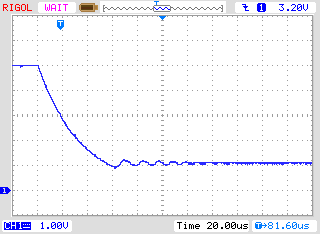
\includegraphics[width=9cm]{../PNG/AREF2_1V.png}
    \caption{from 5V to 1.1V }
    \label{pic:aref1}
  \end{subfigure}
  ~
  \begin{subfigure}[b]{9cm}
    \centering
    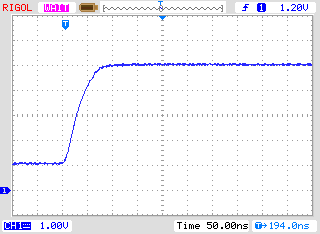
\includegraphics[width=9cm]{../PNG/AREF2VCC.png}
    \caption{from 1.1V to 5V}
    \label{pic:aref5}
  \end{subfigure}
  \caption{Umschalten von AREF mit einem \(1nF\) Kondensator}
\end{figure}

\begin{description}
  \item[REF\_R\_KORR] gibt einen Offset für die interne Referenz-Spannung in mV-Einheiten an.
Mit diesem Offset kann eine Differenz bei der Umschaltung der Referenzspannung für die Widerstandsmessung abgeglichen werden.
Wenn die AUTO\_CAL Option gewählt wurde, ist dieser Wert nur ein Offset zu der gefundenen Spannungs-Differenz in der
AUTO\_CAL Funktion.\\
Beispiel: CFLAGS += -DREF\_R\_KORR=10
  \item[OP\_MHZ] gibt der Software an, mit welcher Taktfrequenz in MHz der Tester arbeiten wird.
Die Software ist nur mit 1MHz, 8MHz und zusätzlich auch 16MHz getestet. Der Betrieb mit 8MHz wird wegen der besseren Auflösung der
Kondensator- und Spulen-Messung empfohlen.\\
Beispiel: OP\_MHZ = 8
  \item[RESTART\_DELAY\_TICS] muß auf 6 gesetzt werden, wenn der ATmega168 oder ATmega328 ohne Quarz mit dem
RC-Generator betrieben wird. Wenn dieser Wert nicht vorbesetzt wird, wählt die Software die 16384 Takte Startverzögerung für
den Quarzbetrieb.\\
Beispiel: CFLAGS += -DRESTART\_DELAY\_TICS = 6
  \item[USE\_EEPROM] gibt an, ob feste Texte und Tabellen im EEprom-Speicher abgelegt werden sollen.
Anderenfalls wird der Programmspeicher (Flash) benutzt.
Es wird empfohlen, den EEprom-Speicher zu benutzen (Option gesetzt).\\
Beispiel: CFLAGS += -DUSE\_EEPROM
  \item[EBC\_STYLE] gibt an, daß die Ausgabe der Transistor Pinbelegung im Format ,,EBC=...'' bzw. ,,GDS=...'' erfolgen soll.
Diese Darstellungsweise spart Programmplatz. Ohne diese Option wird die Belegung im Format ,,123=...'' angezeigt, wobei
jeder Punkt ein E (Emitter), B (Basis) oder K (Kollektor) sein kann.
Bei FET Transistoren kann jeder Punkt entsprechend ein G (Gate), D (Drain) oder S (Source) sein.
Wenn die Reihenfolge der Testpins nicht 1,2 und 3 in Leserichtung ist, kann die Reihenfolge mit der Option EBC\_STYLE=321 
umgedreht werden. Dann wird die Pinbelegung in der Form ,,321=...'', was der gewohnten Leserichtung von links nach rechts
entgegen kommt.\\
Beispiel: CFLAGS += EBC\_STYLE
  \item[NO\_NANO] gibt an, daß der dezimal Präfix Nano nicht zur Darstellung von Meßergebnissen benutzt werden soll.
So werden Kapazitätswerte in \(\mu F\) statt in \(nF\) angegeben.\\
Beispiel: CFLAGS += NO\_NANO
  \item[PULLUP\_DISABLE] gibt an, daß man die internen ,,pull-up'' Widerstände nicht benötigt.
 Sie müssen einen externen ,,pull-up'' Widerstand an Pin 13 (PD7) und VCC angeschlossen haben, um diese
Option benutzen zu können.
Mit dieser Option wird ein möglicher Einfluss der ,,pull-up'' Widerstände auf die Mess-Ports (Port B und Port C) verhindert.\\
Beispiel: CFLAGS += -DPULLUP\_DISABLE
  \item[ANZ\_MESS] diese Option gibt an, wie oft der ADC-Wert eingelesen und addiert werden soll.
Sie können einen Wert zwischen 5 und 200 wählen um einen Mittelwert für eine ADC-Messung zu bilden.
Höhere Werte ergeben eine bessere Genauigkeit, aber brauchen längere Messzeit.
Eine ADC-Messung mit dem Wert 44 braucht etwa 5ms.\\
Beispiel: CFLAGS += -DANZ\_MESS=44
  \item[POWER\_OFF] Diese Option schaltet die automatische Abschaltfunktion ein.
Wenn Sie diese Option weglassen, werden die Messungen in einer Schleife endlos wiederholt, bis die Betriebs-Spannung 
unterbrochen wird (Ein/Aus Schalter).
Wenn Sie einen Tester ohne die Schalttransistoren haben, können Sie diese Option weglassen.

Wenn Sie mit den eingebauten Schalttransistoren die Option POWER\_OFF weggelassen haben,
gibt es dennoch eine Möglichkeit für eine Abschaltung, wenn Sie die WITH\_MENU Option gewählt haben.

Sie können mit der POWER\_OFF Option auch angeben, nach wie vielen Messungen ohne gefundenes Bauteil der Tester ausschaltet.
Bei doppelt so viel aufeinanderfolgenden Messungen mit gefundenem Bauteil schaltet der Tester auch ab,
wenn nicht zwischendurch eine Messung ohne gefundenes Bauteil war.
Wenn Sie vergessen haben, ein angeschlossenes Bauteil abzuklemmen, wird so eine vollständige Batterie-Entladung
verhindert.
Bei einer Options-Angabe in der Form von CFLAGS += -DPOWER\_OFF=5 wird nach 5 aufeinanderfolgenden Messungen ohne
gefundenes Bauteil abschaltet. Aufeinanderfolgende 10 Messungen mit gefundenem Bauteil schalten ebenfalls aus.
Nur wenn die jeweilige Mess-Serie durch den anderen Typ unterbrochen wird, wird die Messung fortgesetzt.
Die Messresultate für eine Einzelmessung werden 28~Sekunden angezeigt, bei der Mehrfachmessung wird die
Anzeigezeit auf 5~Sekunden reduziert (wird in config.h gesetzt).
Wenn der Startknopf beim ersten Einschalten lange gedrückt wird, wird das Messergebnis
 auch bei der Mehrfachmessung 28~Sekunden angezeigt.
Der Maximalwert für die Wiederholungen ist 255 (CFLAGS += -DPOWER\_OFF=255).\\
Beispiel 1: CFLAGS += -DPOWER\_OFF=5 \\
Beispiel 2: CFLAGS += -DPOWER\_OFF 
  \item[BAT\_CHECK] schaltet die Batterie Spannungsprüfung ein.
 Wenn Sie diese Option nicht angeben, wird die Versions-Nummer der Software angezeigt.
Diese Option ist hilfreich um bei Batterie betriebenen Tester Versionen an den Batterie Wechsel zu erinnern.\\
Beispiel: CFLAGS += -DBAT\_CHECK
  \item[BAT\_OUT] schaltet die Batterie-Spannungsanzeige auf dem LCD ein, wenn BAT\_CHECK gewählt wurde.
 Wenn Ihre 9V-Versorgung eine Diode wegen des Verpolungs-Schutzes installiert hat, können Sie 
die Form BAT\_OUT=600 angeben, um die Dioden-Schwellspannung 
bei der Spannungsanzeige zu berücksichtigen.
Auch der Spannungsverlust am Transistor T3 kann so mit dieser Option berücksichtigt werden.
Die Angabe der Schwellspannung in mV beeinflusst nicht die Prüf\-span\-nungs Werte (BAT\_POOR).\\
Beispiel 1: CFLAGS += -DBAT\_OUT=300 \\
Beispiel 2: CFLAGS += -DBAT\_OUT
  \item[BAT\_POOR] setzt die Leer-Spannung für die Batteriespannungs-Prüfung auf den angegebenen Wert in Einheiten von 1mV.
Die Warn-Spannung ist 0.8V höher als die angegebene Leer-Spannung, wenn die Leer-Spannung mehr als 5.3V beträgt.
Sonst wird eine 0.4V höhere Warn-Spannung gewählt, bei unter 3.25V sogar nur eine 0.2V höhere Warn-Spannung und
bei unter 1.3V nur eine 0.1V höhere Warnspannung als die angegebene Leer-Spannung.
Das Setzen der Leer-Spannung auf Werte wie 5,4V wird für wiederaufladbare 9V Batterien nicht empfohlen,
weil das die Gefahr von Batterie-Schäden wegen der Tief-Entladung erhöht!
Wenn Sie wiederaufladbare 9V Batterien einsetzen, werden ,,Ready to Use'' Typen wegen der geringeren Selbstentladung empfohlen.\\
Beispiel für low drop Regler (5.4V): CFLAGS += -DBAT\_POOR=5400 \\
Beispiel für 7805 type Regler (6.4V): CFLAGS += -DBAT\_POOR=6400
  \item[INHIBIT\_SLEEP\_MODE] sperrt die Benutzung des ,,Sleep Modus'' (Schafzustand) des Prozessors.
Normalerweise wird von der Software für längere Pausen der Schlafzustand des Prozessors benutzt, um Strom zu sparen.
Die Benutzung dieses Schlafzustandes mit dem Wiederaufwachen spart zwar Batteriekapazität, 
stellt eine zusätzliche Anforderung für den Spannungsregler dar.\\
Beispiel: CFLAGS += -DINHIBIT\_SLEEP\_MODE
  \item[PROGRAMMER] stellt den Programmer Typ für das avrdude Schnittstellenprogramm ein.
Eine richtige Einstellung des Programmer Typs (und Ports) ist notwendig, wenn Sie den ,,make upload'' oder
,,make fuses'' Aufruf dieser Makefile benutzen.
Für weitere Informationen schauen Sie bitte in das Handbuch von avrdude oder in die Online-Dokumentation~\cite{avrdude}.\\
Beispiel: PROGRAMMER=avrisp2
  \item[BitClock] stellt die Bit Taktperiode für den Programmer ein. Siehe dazu die Beschreibung des -B Parameters von avrdude.\\
Beispiel: BitClock=5.0
  \item[PORT] stellt die verwendete Schnittstelle ein, wo avrdude den Mikrocontroller (ATmega) erreichen kann.
Für weitere Informationen schauen Sie bitte ins Handbuch von avrdude.\\
Beispiel: PORT=usb

\end{description}

Zusätzliche Parameter können in den Dateien Transistortester.h und config.h gesetzt werden.
Die Datei config.h enthält globale Variablen und Tabellen, definiert die Port- / Pin-Konstellation,
die ADC-Taktfrequenz sowie die Widerstandswerte, die für die Messung benutzt werden.
Die Datei Transistortester.h enthält die globalen Variablen und Tabellene sowie die Texte für die LCD-Anzeige.
Normalerweise brauchen diese Werte nicht ohne Grund geändert werden.


\chapter{Beschreibung des Messverfahrens}
\label{sec:measurement}
Ein vereinfachtes Schaltbild eines Eingangs-/Ausgangs-Pin des ATmega wird in Abbildung~\ref{fig:port} gezeigt.
Der Schalter PUD schaltet die Versorgung für alle ,,Pull Up''-Widerstände des ATmega ab.
Mit dem Schalter DD kann der Ausgang abgeschaltet werden, der Eingang funktioniert sowohl im Ausgabe- wie im
Eingabe-Modus. Im Eingabe-Modus wird mit dem Ausgabewert (PORT) der ,,Pull Up''-Widerstand des Eingangs mit geschaltet.
Die beiden Schalter PORT und DD können nicht gleichzeitig, sondern nur nacheinander geschaltet werden.
Weil beim Umschalten der ,,Pull Up'' Widerstand die Messung stören könnte, bevorzuge ich die komplette
Abschaltung aller ,,Pull Up'' Widerstände mit dem PUD-Schalter.
Natürlich sind die Schalter elektronisch und die Widerstände \(19\Omega\) und \(22\Omega\) sind angenäherte Werte.
\begin{figure}[H]
\centering

\includegraphics[]{../FIG/port.eps}
\caption{Vereinfachtes Schaltbild jedes ATmega-Portpins}
\label{fig:port}
\end{figure}

Jeder der drei Testpins Ihres TransistorTesters wird aus drei ATmega-Portpins gebildet,
was im vereinfachten Schaltbild des Testpins TP2 (mittlerer der drei Pins) in Abbildung~\ref{fig:terminal} gezeigt wird.

\begin{figure}[H]
\centering

\includegraphics[]{../FIG/terminal.eps}
\caption{Vereinfachtes Schaltbild des Testpins TP2}
\label{fig:terminal}
\end{figure}

Jeder Testpin (Messport) kann als digitaler oder analoger Eingang benutzt werden.
Diese Mess\-fähig\-keit ist un\-abhän\-gig von der Verwendung des Ports als Ausgang.
Jeder Testpin kann als Ausgang verwendet werden und in diesem Zustand mit GND (0V) oder VCC (5V) verbunden werden,
oder er kann über die Widerstände (\(680\Omega\) oder \(470k\Omega\)) mit entweder GND oder VCC verbunden werden.
Tabelle \ref{tab:case} zeigt alle denkbaren Messmöglichkeiten.
Beachten Sie, dass der positive Zustand durch direktes Verbinden mit VCC (Port C) oder
durch Verbinden mit dem \(680\Omega\) Widerstand mit VCC (Port B) erreicht werden kann.
Die gleiche Möglichkeit hat der negative Zustand des Testpins zu der GND-Seite.
Der Test-Zustand meint, dass der Pin offen sein kann (Eingang), verbunden "uber den \(470k\Omega\)-Widerstand
mit VCC oder GND, oder der Pin kann "uber den \(680\Omega\)-Widerstand mit VCC oder GND verbunden sein.

\begin{table}[H]
  \begin{center}
    \begin{tabular}{| l | c | c | c |}
    \hline
      & Zustand Pin 1 & Zustand Pin 2 & Zustand Pin 3 \\
    \hline
   1. & positiv    &  negativ   &  test \\
   2. & positiv    &  test      & negativ \\
   3. & test       &  negativ   & positiv \\
   4. & test       &  positiv   & negativ \\
   5. & negativ    &  test      & positiv \\
   6. & negativ    &  positiv   &  test  \\
    \hline
    \end{tabular}
  \end{center}
  \caption{alle Messmöglichkeiten}
  \label{tab:case} 
\end{table}

Wenn die Kondensatormessung des Testers konfiguriert ist, versucht der Tester vor allen Messungen erst einmal,
die Kondensatoren an allen Anschlusspins zu entladen. Wenn das nicht gelingt, also die Restspannung zu hoch bleibt,
wird das Entladen nach etwa 12 Sekunden mit der Meldung ,,Cell!'' abgebrochen. Dies kann auch dann vorkommen, wenn
gar kein Kondensator angeschlossen ist. Die Ursache kann in diesem Fall sein, dass die Entlade-Grenzspannung für diesen
ATmega zu niedrig gewählt ist. Man kann eine höhere Restspannung mit der Makefile Option CAP\_EMPTY\_LEVEL wählen.


 %\newpage
\section{Messung von Halbleitern}
Als erster Test soll der Stromfluß des Bauteils bei stromlosen Steuerpin (dritter Pin, auch TriStatePin genannt)
untersucht werden. Der Steuerpin ist beispielsweise das Gitter oder die Basis des Testobjektes.
Ein Testpin wird die positive Seite des Bauteils angenommen und direkt mit VCC verbunden.
Ein anderer Pin wird als negative Seite des Bauteils angenommen.
Die negative Seite wird mit dem \(680\Omega\) Widerstand nach GND verbunden.
Bei Feldeffekt Transistoren ist der Zustand des Transistors von der Spannung des Gitters abhängig.
Der Tristatepin wird zuerst mit dem \(680\Omega\)-Widerstand für 5ms mit GND verbunden und
die Spannung an der negativen Seite gemessen.
Danach wird die Spannung des negativen Testpins wieder gemessen, während der TriStatePin auf
Eingang (hochohmig) geschaltet ist.
Danach wird das angenommene Gate für 5ms mit dem \(680\Omega\)-Widerstand auf VCC geschaltet 
und die Spannung an der negativen Seite noch einmal gemessen.
Wenn die gemessene Spannung jetzt niedriger ist als bei der ersten Messung, wird diese Schaltung
als richtig angenommen. Dann wird die Spannung noch einmal mit stromlosen TristatePin gemessen.

Wenn die Spannung des negativen Pins mit festgehaltenem Pegel größer als \(115 mV\) ist
und dieser Pegel nicht \(100 mV\) niedriger als der Pegel mit stromlosen TristatePin ist,
wird ein Verarmungs-Typ angenommen.
Bei bipolaren Transistoren mit hohem Reststrom ist
der Kollektor-Reststrom bei stromloser Basis deutlich höher.
Durch die Überprüfung beider Pegel wird eine Falschdetektion von Germanium Transistoren mit
höheren Kollektor-Reststroms als Verarmungs Transistoren (JFET) vermieden.
Es werden dann weitere Tests gemacht,
um N-Kanal JFET oder D-MOSFET  und P-Kanal JFET oder P-MOSFET zu unterscheiden.
Die MOSFET-Versionen können erkannt werden durch das Fehlen von Steuerstrom in jedem 
TriStatePins Zustand.

Um Parameter der Verarmungstypen messen zu können, werden sie mit einem \(680 \Omega\)-Widerstand am
Source-Pin vermessen, wie in Abbildung \ref{fig:JFETcd} gezeigt wird. Diese Messung wird anstelle der
üblichen Messung des Stromes bei einer Gate-Spannung auf Source-Potential gemacht, da wegen des
relativ hohen \(680 \Omega\) Widerstandes in vielen Fällen der Kennstrom \(I_\mathrm{DSS}\) 
des FETs nicht erreicht würde.

\begin{figure}[H]
\centering

\includegraphics[]{../FIG/JFETcd.eps}
\caption{Messung von Gate-Source-Spannung und Source-Strom eines N-JFET-Transistors}
\label{fig:JFETcd}
\end{figure}

Wenn das Bauteil keinen Strom zwischen dem positiven Pin und dem negativen Pin ohne ein Signal
auf dem TristatePin hat, sind die nächsten Tests im nächsten Unterkapitel \ref{sec:pnp} beschrieben.
Wenn Strom festgestellt wird, sind die nächsten Tests in dem Dioden-Unterkapitel \ref{sec:diode} beschrieben.

\subsection{Messung eines PNP-Transistors oder eines P-Kanal MOSFETs}
\label{sec:pnp}
Zuerst wird der Stromverstärkungsfaktor in der Kollektor-Schaltung (Emitter-Folger) für den angenommenen
PNP-Transistor gemessen.
Die Messsituation wird in Abbildung \ref{fig:pnpcc} gezeigt.
Wenn die gemessene Basis-Spannung (\(UB\)) über 9mV mit dem \(680\Omega\) Widerstand liegt,
wird die Stromverstärkung hFE berechnet mit \(hFE = \frac{UE-UB}{UB}\). 
Die Spannung \(UE\) ist die Differenz der Emitter-Spannung zu VCC.
Die Differenz des \(22\Omega\) und \(19\Omega\)-Widerstandes wird nicht berücksichtigt.
Wenn die Spannung \(UB\) unter 10mV liegt, wird die Messung mit dem \(470k\Omega\)-Widerstand an der Basis gemacht.
Für diesen Fall wird der Stromverstärkungsfaktor mit \(hFE = \frac{UE \cdot 470000}{UB \cdot (680+22)}\) gebildet.

\begin{figure}[H]
\centering

\includegraphics[]{../FIG/PNPcc.eps}
\caption{hFE-Messung eines PNP-Transistors in Kollektor-Schaltung}
\label{fig:pnpcc}
\end{figure}

Als Nächstes werden die Tests in Emitter-Schaltung für den angenommenen PNP-Transistor gemacht.
Die positive Seite wird jetzt direkt mit VCC verbunden, der \(680\Omega\)-Widerstand der negativen Seite wird 
mit GND verbunden, wie es in Abbildung \ref{fig:pnpce} gezeigt wird. 
Wenn die negative Seite des Bauteils eine Spannung über 3,4V hat, wenn der \(680\Omega\)-Widerstand auf der Basis-Seite mit
GND verbunden ist, muss es ein PNP-Transistor oder ein P-Kanal-FET sein.
Das kann einfach unterschieden werden durch Prüfen der Basis-Spannung: Wenn sie grösser als 0,97V ist, muss es ein PNP sein.
Für die Messung des Stromverstärkungsfaktors wird anstelle des \(680\Omega\)-Widerstandes der
 \(470k\Omega\)-Widerstand als Basis-Widerstand genommen.
Der Stromverstärkungsfaktor wird berechnet mit \(hFE = \frac{(UC-UC0) \cdot 470000}{UB \cdot (680+19)}\) .
Die Spannung UC0 ist die Spannung am Kollektorwiderstand ohne Basisstrom.
Der höhere Stromverstärkungsfaktor wird als der richtige angenommen, dieser hier oder der
mit der Kollektor-Schaltung bestimmte.


Die Werte, die für den PNP-Transistor herausgefunden wurden, sind nur gültig, wenn ein zweiter Satz
von Messungen gemacht wurde.
Um zu verhindern, dass der PNP-Transistor in der inversen Schaltung (Kollektor und Emitter vertauscht) erkannt
wird, wird dann die Messung mit dem höheren Stromverstärkungsfaktor als richtige Messung genommen.
Wenn die Basis-Spannung kleiner als 0,97V ist, muss es ein P-E-MOS sein.
In diesem Fall wird die Gate-Schwellwertspannung dadurch bestimmt, dass die Spannung am Gate langsam mit dem
 \(470k\Omega\)-Widerstand rauf und runter gezogen wird bis die Drain-Seite schaltet und dann
die Spannung am Gate gemessen wird.

\begin{figure}[H]
\centering

\includegraphics[]{../FIG/PNPce.eps}
\caption{Prüfung und hFE-Messung eines PNP-Transistors in der Emitter-Schaltung}
\label{fig:pnpce}
\end{figure}

\subsection{Messung eines NPN-Transistors oder eines N-Kanal-MOSFET}
Die Messung eines NPN-Transistors beginnt auf gleiche Weise wie die PNP-Transistor-Messung, nämlich
mit der Messung des Stromverstärkungsfaktors in der Kollektor-Schaltung.
Zuerst wird die Messung mit einem nach VCC geschalteten \(680\Omega\)-Basiswiderstand gemacht.
Wenn die Spannung am Basis-Widerstand zu klein ist, wird stattdessen der \(470k\Omega\)-Widerstand genommen.
Die Messungen werden dann in der Emitter-Schaltung fortgeführt, wie in Abbildung \ref{fig:npnce} gezeigt.
\begin{figure}[H]
\centering

\includegraphics[]{../FIG/NPNce.eps}
\caption{Prüfung und hFE-Messung eines NPN-Transistors in Emitter-Schaltung}
\label{fig:npnce}
\end{figure}
Wenn die Spannung auf der Kollektor Seite unter 1,6V liegt, während der \(680\Omega\)-Basiswiderstand mit
VCC verbunden ist, muss es ein NPN, ein N-Kanal MOSFET oder ein Thyristor (TRIAC) sein.
Mit zwei einfachen Tests kann ein Thyristor oder Triac erkannt werden.
Wenn der Gate-Pin für 10ms mit GND verbunden wird und dann stromlos geschaltet wird, sollte
der Strom an der Anode bleiben.
Wenn jetzt der Anoden-Widerstand kurz auf GND geschaltet und dann auf VCC zurückgeschaltet wird,
sollte der Thyristor nicht erneut zünden (stromlos bleiben).
Beachten Sie, dass nur Kleinleistungs Thyristoren getestet werden können, weil der Haltestrom des
Testers nur 6mA erreichen kann.
Wenn beide Tests einen Thyristor bestätigen, werden weitere Tests in umgekehrter Polarität gemacht,
um ein TRIAC auszuschliessen oder zu bestätigen.

Wenn weder Thyristor noch TRIAC bestätigt wurden, kann es ein NPN oder ein N-Kanal E-MOSFET sein.
Die Basis-Spannung von einem NPN-Transistor wird nahe bei der Emitter-Spannung liegen, so dass dieser Typ sicher
erkannt werden kann.
Der Stromverstärkungsfaktor in der Emitter-Schaltung wird durch 
\(hFE = \frac{(VCC-UC-UC0)\cdot 470000}{(VCC-UB)\cdot (680+22)}\) gebildet.
Wenn die Spannung an der Basis zeigt, dass kein oder wenig Strom fließt, wird das Bauteil ein N-Kanal E-MOS
(Anreicherungs-MOSFET) sein.
In diesem Fall wird die Schwellspannung gemessen, indem die Spannung des Gates langsam mit
dem \(470k\Omega\)-Widerstand nach VCC und GND gezogen wird, darauf wartend, dass das digitale
Eingangs-Signal auf der Drain Seite schaltet, wobei dann die Gate-Spannung gelesen wird.
Die Messung wird elf Mal wiederholt wie in Abbildung~\ref{fig:eleven} gezeigt und die Ergebnisse addiert.
Diese Summe wird mit vier multipliziert und durch neun geteilt um eine Auflösung in mV zu erhalten.
\begin{figure}[H]
\centering
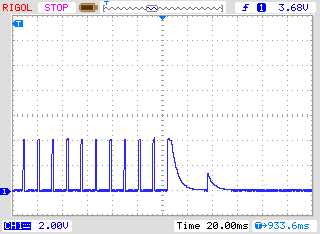
\includegraphics[]{../PNG/IRFU120gate.png}
\caption{Messung der Schwellspannung eines N-Kanal-MOSFET}
\label{fig:eleven}
\end{figure}

\subsection{Vereinfachter Ablauf der Transistorerkennung}

\begin{figure}[H]
\centering

\includegraphics[]{../FIG/CheckSemi1.eps}
\caption{Ablaufplan der Transistorprüfung Teil 1, JFET und D-MOS}
\label{fig:ChkSemi1}
\end{figure}

\begin{figure}[H]
\centering

\includegraphics[]{../FIG/CheckSemi2.eps}
\caption{Ablaufplan der Transistorprüfung Teil 2, BJT und E-MOS}
\label{fig:ChkSemi2}
\end{figure}

\begin{figure}[H]
\centering

\includegraphics[]{../FIG/CheckSemi3.eps}
\caption{Ablaufplan der Transistorprüfung Teil 3, Thyristor und Triac}
\label{fig:ChkSemi3}
\end{figure}

\subsection{Messung von Dioden}
\label{sec:diode}
Wenn Strom bei den Vortests festgestellt wurde, wird das Bauteil auf Diodenverhalten geprüft.
Die Flussspannung mit dem \(680\Omega\)-Widerstand muss zwischen 0,15V und 4,64V liegen.
Die Flussspannung mit dem \(680\Omega\)-Widerstand muss grösser als 1,125 Mal der Flussspannung mit dem
 \(470k\Omega\)-Widerstand sein und sechzehn Mal die Flussspannung mit dem \(470k\Omega\)-Widerstand muss
grösser als die Flussspannung mit dem \(680\Omega\)-Widerstand sein.
Zusätzlich darf die anschließende nochmalige Messung mit dem \(470k\Omega\)-Widerstand  keine höhere Spannung als die
Messung mit dem \(680\Omega\)-Widerstand ergeben.
Ich hoffe, dass ein Bauteil mit diesem Verhalten immer eine Diode ist.
Die Erkennung des Diodenverhaltens durch den fehlenden Stromfluß in der Gegenrichtung ist nicht
möglich bei antiparallelen Dioden.
Bei einer Einzeldiode wird zusätzlich der Sperrstrom der Diode bei 5V mit dem \(470k\Omega\) Widerstand
gemessen. Die Auflösung beträgt etwa \(2nA\).
Bei größeren Restströmen als \(5.3\mu A\) (Spannung am Widerstand größer als 2.5V) wird
 mit dem \(680\Omega\) Widerstand gemessen.
Dann beträgt die Auflösung nur etwa \(1\mu A\).
Außerdem wird bei Einzeldioden eine Kapazitätsmessung in Sperr-Richtung durchgeführt. 

\subsection{Ergebnisse der verschiedenen Messungen}
Die folgenden drei Tabelle zeigen die Ergebnisse verschiedener Bauteile 
eines ATmega8-Prozessors, eines ATmega168 und eines ATmega328 Prozessors.
Die Messung der Sperrschichtkapazität für die Doppeldiode MBR4045PT gelingt
nur gekühlt. Die Ursache hierfür ist der hohe Reststrom der 40A Diode. Ebenso kann für die Basis - Emitter
Strecke des Germanium Transistors AC128 die Sperrschichtkapazität nur im
gekühlten Zustand gemessen werden. 

\begin{table}[H]
  \begin{center}
    \begin{tabular}{| l | c | c | c | c |}
    \hline
           & Mega8@8MHz          & Mega168 @8MHz       & Mega328 @8MHz     \\
 Diode Typ &                     &                     &                   \\
    \hline
    \hline
1N4148     & Diode, 715mV,        & Diode, 718mV,            & Diode, 715mV,           \\
           &               1pF    &               0pF, 2nA   &               1pF, 4nA  \\
    \hline
1N4150     & Diode, 665mV,        & Diode, 672mV,            & Diode, 666V,           \\
           &               1pF    &               1pF, 4nA   &              2pF, 6nA  \\
    \hline
BA157      & Diode, 619mV,        & Diode, 621V,              & Diode, 615mV,            \\
           &               19pF   &              17pF, 12nA   &               18pF, 12nA \\
    \hline
BY398      & Diode, 538mV,        & Diode, 541mV,             & Diode, 537mV,            \\
           &               16pF   &               14pF, 63nA  &               15pF, 63nA \\
    \hline
1N4007     & Diode, 650mV,        & Diode, 655mV,            & Diode, 650mV,           \\
           &               13pF   &               10pF, 6nA  &               13pF, 6nA \\
    \hline
LED green  & Diode, 1.96V, 5pF    & Diode, 1.95V, 4pF   & Diode, 1.95V, 4pF \\
    \hline
ZPD2,7     & 2xDi, 743mV, 2.53V   & 2xDi, 737mV, 2.52V  & 2xDi, 733mV, 2.51V \\
    \hline
BU508A B+E & Diode, 609mV,        & Diode, 611mV,                & Diode, 606mV,              \\
           &               5.15nF &               5.20nF, 0.39uA &               5.25nF, 0.4uA\\
    \hline
BU508A B+C & Diode, 582mV,        & Diode, 586mV,             & Diode, 587mV,            \\
           &               256pF  &               255pF, 21nA &               259pF, 19nA\\
    \hline
AC128 B+E  & Diode, 272mV,        & Diode, 277mV,              & Diode, 273mV,             \\
           &               0pF    &               0pF, 2.2uA   &               0pF, 2.3uA  \\
    \hline
AC128 B+E  &                      &                     & Diode, 349mV,               \\
gekühlt    &                      &                     &               140pF, 0.57uA \\
    \hline
MBR20100CT & 2xDi, 337mV, 337mV   & 2xDi, 338mV, 338mV  & 2xDi, 336mV, 335mV  \\
    \hline
MBR20100CT & Diode, 337mV,        & Diode, 339mV,             & Diode, 337mV,            \\
           &               345pF  &               351pF, 29nA &               350pF, 25nA\\
    \hline
MBR4045PT  & Diode, 243mV,        & Diode, 233mV,               & Diode, 235mV,              \\
gekühlt    &               1.80nF &               1.94nF, 1.7uA &               1.95nF, 1.8uA\\
    \hline
SK14       & Diode,    mV,        & Diode,    mV,               & Diode, 263mV,              \\
           &                  0pF &                   pF,    nA &               0pF, 0.57uA\\
    \hline
SK14       & Diode,    mV,        & Diode,    mV,               & Diode, 334mV,              \\
gekühlt    &                   nF &                   pF,    nA &               88pF, 4nA\\
    \hline
SF38G      & Diode, 519mV,        & Diode, 521mV,            & Diode, 516mV,            \\
           &               107pF  &               105pF, 2nA &               106pF, 2nA \\
    \hline
    \end{tabular}
  \end{center}
  \caption{Messergebnisse der Dioden-Tests}
  \label{tab:diodes} 
\end{table}

\begin{table}[H]
  \begin{center}
    \begin{tabular}{| l | c | c | c | c | c |}
    \hline
 Transistor & Typ & Mega8           & Mega328        & Mega328         & Mega328 \\
    Typ     &     & common-         & maximum        & common-         & common- \\
            &     & collector       &                & collector       & emitter \\
    \hline
    \hline
BU508A      & NPN & B=9, 601mV      &  B=9, 597mV    &   B=9, 598mV    & B=4, 484mV \\
    \hline
2N3055      & NPN & B=20, 557mV     &  B=21, 550mV   &   B=21, 550mV   & B=6, 442mV \\
    \hline
BC639       & NPN & B=148, 636mV    &  B=172, 629mV  &   B=172, 629mV  & B=158, 605mV \\
    \hline
BC640       & PNP & B=226, 650mV    &  B=176, 609mV  &   B=171, 655mV  & B=177, 608mV \\
    \hline
BC517       & NPN & B=23.9k, 1.23V  &  B=24.8k, 1.22V&   B=25.1k, 1.22V & B=764, 1.23V \\
    \hline
BC516       & PNP & B=75.9k, 1.21V  &  B=76.2k, 1.20V&   B=76.2k, 1.20V & B=760, 1.23V \\
    \hline
BC546B      & NPN & B=285, 694mV    &  B=427, 687mV  &   B=427, 687mV   & B=369, 683mV \\
    \hline
BC556B      & PNP & B=304, 704mV    &  B=254, 668mV  &   B=235, 709mV   & B=255, 668mV \\
    \hline
AC128 (Ge.) & PNP & B=63, 191mV     &  B=59, 191mV   &   B=57, 193mV    & B=43, 117mV \\
    \hline
BUL38D      & NPNp & B= 37, 627mV    &  B=41, 617mV  &   B=40, 624mV    & B=36, 562mV \\
parasitär   & PNPn & B= 11, 654mV    &  B=81, 543mV  &   B=10, 656mV    & B=83, 541mV \\
    \hline
BRY55/200   & Thyrist. &  0.84V      &  0.81V        &  0.82V           &  0.82V \\
    \hline
MAC97A6     & Triac &   0.92V        &  0.90V        &  0.91V           &  0.90V    \\
    \hline
    \end{tabular}
  \end{center}
  \caption{Messergebnisse der Tests mit bipolaren Transistoren}
  \label{tab:bipolar} 
\end{table}

Die Ergebnisse der Transistormessungen unterscheiden sich teilweise erheblich von den Werten der Version 
von Markus Frejek. Zum Beispiel wird für den Darlington Transistor BC517 von
der früheren Software ein hFE von nur 797 statt 77200 gemessen. 
Dies hängt damit zusammen, dass die Stromverstärkung bei der neuen Version auch mit der
Kollektorschaltung gemessen wird.
Dies zeigen auch die Ergebnisse der neuen Version in der Emitterschaltung (common emitter),
wie man in der letzten Spalte der Tabelle \ref{tab:bipolar} sehen kann.
Die Basis Emitter Spannung wurde früher mit einem separaten Diodentest mit 1438mV ermittelt.
Jetzt wird die angegebene Basis Emitter Spannung im Zustand der Verstärkungsmessung (1.20V) ermittelt.
Der BUL38D Transistor enthält eine Schutzdiode über der Anode und dem Kollektor des NPN Transistors,
wodurch ein parasitärer PNP Transistor mit vertauschtem Basis - Kollektor Anschluß entsteht.
In der Softwareversion 1.10k werden beide Transistoren erkannt und durch das angehängte p auf
den weiteren Transistor hingewiesen.
Der richtige Transistor (NPN) wird durch einen Vergleich der Sperrschichtkapazitäten herausgefunden.
Es wird angenommen, daß der mit der höheren Sperrschichtkapazität der richtige Transistor ist.
Wenn während der Ergebnisanzeige die Start-Taste gedrückt ist, werden die Parameter des parasitären Transistors
angezeigt. Dabei wird wieder mit PNPn auf die andere Transistorstruktur hingewiesen.
Die weitere Transistorstruktur entsteht nur bei der Integration der Schutzdiode in unmittelbarer
Nachbarschaft des Transistors in das gleiche Halbleitermaterial, nicht bei einer externen Diode.

In der folgenden Tabelle \ref{tab:germanium} werden die Meßergebnisse von Germanium Transistoren gezeigt, die wegen den
stark Temperatur abhängigen Kollektor Restströmen besonders problematisch sind.
Es werden die Ergebnisse der Urversion von Markus F. und die Ergebnisse der aktuellen 1.10k Version
miteinander verglichen. Die 1.10k Version mißt die Stromverstärkung sowohl in der
Kollektorschaltung als auch in der Emitterschaltung mit Berücksichtigung des Kollektor-Ruhestroms,
 wobei die höhere Stromverstärkung ausgegeben wird.
Der Kollektor-Ruhestrom wurde in älteren Versionen nicht berücksichtigt.

\begin{table}[H]
  \begin{center}
    \begin{tabular}{| l | c | c | c |}
    \hline
 Transistor & Mega8@1MHz          & Mega168 @8MHz       & Mega328 @8MHz    \\
    Typ     & Ur-Version          & Version 1.10k       & Version 1.10k  \\
            & Markus F.           &                     &        \\
    \hline
    \hline
AC128       & PNP, B=52, 279mV    & PNP, B=59, 184mV    & PNP, B=59, 191mV    \\
    \hline
AC116-65    & PNP, B=505, 378mV   & PNP, B=72, 146mV    & PNP, B=72, 149mV    \\
    \hline
AC116-145   & PNP, B=485, 294mV   & PNP, B=146, 161mV    & PNP, B=146, 163mV   \\
    \hline
AC176-65    & NPN, B=98, 235mV    & NPN, B=58, 94mV    & NPN, B=56, 96mV     \\
    \hline
GC122       & PNP, B=84, 368mV    & PNP, B=55, 117mV    & PNP, B=56, 117mV    \\
    \hline
GC301       & PNP, B=48, 289mV    & PNP, B=39, 184mV    & PNP, B=39, 188mV    \\
    \hline
AD161       & NPN, B=360, 230mV   & NPN, B=296, 126mV   & NPN, B=298, 128mV    \\
    \hline
AD162       & PNP, B=2127, 280mV  & PNP, B=89, 107mV    & PNP, B=89, 107mV    \\
    \hline
    \end{tabular}
  \end{center}
  \caption{Messergebnisse der Tests mit bipolaren Germanium Transistoren}
  \label{tab:germanium} 
\end{table}

In der Tabelle \ref{tab:mos} werden die Ergebnisse einiger Feldeffekt-Transistoren Messungen gezeigt.
Ein gemessenen Parameter der E-MOS Typen ist Gate-Source Schaltspannung,
bei der das digitale Eingangssignal des ATmega eines am \(680\Omega\) Drain Widerstand 
angeschlossenen Signals schaltet.
Der andere Parameter ist die gemessenen Gate Kapazität.
Bei sehr schneller Änderung der Gate Spannung wegen einer kleinen Gate Kapazität 
ist die ermittelte Spannung etwas ungenau.
Beim BS250 ändert sich die Gate Spannung von 2.6V auf 2.5V, wenn man einen zusätzlichen
\(10nF\) Kondensator an das gate - source anschließt.
Bei JFET Transistoren wird in den Datenblättern oft der Idss Kennstrom genannt,
der Strom im Drain bei Gate-Source Spannung 0V.
Hier wird aber der Strom angegeben, der sich durch einen \(680\Omega\) Lastwiderstand auf der
Source Seite des JFET ergibt.
Der Lastwiderstand erzeugt für das Gate eine Gegenspannung Vgs,
die ebenfalls angegeben wird.
Wegen des symmetrischen Aufbaus der JFET Transistoren kann Drain und Source nicht unterschieden werden.

\begin{table}[H]
  \begin{center}
    \begin{tabular}{| l | l | c | c | c |}
    \hline
             &         & Mega8@8MHz       & Mega168 @8MHz    & Mega328 @8MHz \\
 Transistor  & Typ     &                  &                  &               \\
    \hline
    \hline
ZVNL120A     & N-E-MOS & D, 1.6V, 147pF   & D, 1.5V,141pF    & D, 1.5V, 140pF \\
    \hline
IRF530N      & N-E-MOS & D, 3.6V, 1.55nF  & D, 3.6V, 1.54nF  & D, 3.6V, 1.54nF \\
    \hline
BS170        & N-E-MOS & D, 2.6V, 78pF    & D, 2.6V, 68pF    & D, 2.6V, 68pF \\
    \hline
IRL3803      & N-E-MOS & D, 2.3V, 9.81nF  & D, 2.3V, 9.71nF  & D, 2.3V, 9.74nF \\
    \hline
IRFU120N     & N-E-MOS & D, 4.2V, 909pF   & D, 4.2V, 913pF   & D, 4.2V, 911pF \\
    \hline
BUZ71A       & N-E-MOS & D, 3.2V, 714pF   & D, 3.2V, 708pF   & D, 3.2V, 705pF \\
    \hline
ZVP2106A     & P-E-MOS & D, 3.2V, 122pF   & D, 3.2V,115pF    & D, 3.2V, 116pF \\
    \hline
IRF5305      & P-E-MOS & D, 3.6V, 2.22nF  & D, 3.6V, 2.22nF  & D, 3.6V, 2.22nF \\
    \hline
BS250        & P-E-MOS & D, 2.6V, 53pF    & D, 2.6V, 43pF    & D, 2.6V, 44pF \\
    \hline
IRFU9024     & P-E-MOS & D, 3.5V, 937pF   & D, 3.6V, 945pF   & D, 3.5V, 933pF \\
    \hline
J310         & N-JFET  & 3.1mA Vgs=2.2V   & 3.1mA Vgs=2.2V   & 3.1mA Vgs=2.2V \\
Idss=24-60mA &         &                  &                  &              \\
    \hline
2N5459       & N-JFET  & 2.1mA Vgs=1.5V   & 2.1mA Vgs=1.5V   & 2.1mA Vgs=1.5V \\
Idss=4-16mA &          &                  &                  &              \\
    \hline
BF256C       & N-JFET  & 3.4mA Vgs=2.4V   & 3.4mA Vgs=2.4V   & 3.4mA Vgs=2.4V \\
Idss=11-18mA &         &                  &                  &              \\
    \hline
BF245A       & N-JFET  & 1.1mA Vgs=.75V   & 1.1mA Vgs=0.75V  & 1.1mA Vgs=0.75V \\
Idss=2-6mA   &         &                  &                  &              \\
    \hline
BF245B       & N-JFET  & 2.5mA Vgs=1.7V   & 2.5mA Vgs=1.7V   & 2.5mA Vgs=1.7V \\
Idss=6-15mA  &         &                  &                  &              \\
    \hline
BF245C       & N-JFET  & 3.9mA Vgs=2.7V   & 3.9mA Vgs=2.7V   & 3.9mA Vgs=2.7V \\
Idss=12-25mA &         &                  &                  &              \\
    \hline
J175        & P-JFET   & 3.2mA Vgs=2.2V   & 3.2mA Vgs=2.2V   & 3.2mA Vgs=2.2V \\
Idss=7-60mA &          &                  &                  &              \\
    \hline
2N5460      & P-JFET   & 0.78mA Vgs=0.54V & 0.77mA Vgs=0.54V & 0.78mA Vgs=0.54V \\
Idss=1-5mA  &          &                  &                  &              \\
    \hline
BSS139      & N-D-MOS  & 1.7mA Vgs=1.2V  & D, 1.7mA Vgs=1.2V & D, 1.7mA Vgs=1.2V \\
    \hline
BSS169      & N-D-MOS  & 2.6mA Vgs=1.8V  & D, 2.6mA Vgs=1.8V & D, 2.6mA Vgs=1.8V \\
    \hline
GP07N120    & N-E-IGBT & C=3.81nF Vt=4.2V & C=3.76nF Vt=4.2V & C=3.74nF Vt=4.2V \\
    \hline
    \end{tabular}
  \end{center}
  \caption{Messergebnisse der FET-Transistor-Tests}
  \label{tab:mos} 
\end{table}

 %\newpage
\section{Widerstands-Messung}
Jeder Widerstand wird mit vier verschiedenen Messmethoden in einer Stromrichtung vermessen.
Der gleiche Widerstand wird auch mit den gleichen vier Messmethoden in die andere Stromrichtung vermessen.
Die Messung in die Gegenrichtung wird nur für die Erkennung auf Widerstand benutzt.
Wenn die Abweichung dieser beiden Messungen zu groß ist, ist es kein Widerstand.

\subsection{Widerstandsmessung mit den 680-Ohm-Widerständen}
Die Messung des unbekannten Widerstandes Rx wird in zwei verschiedenen Wegen mit den \(680\Omega\)-Präzisionswiderständen
 durchgeführt.
Das Schaltbild dieser Messungen mit Testpin 1 (TP1) und Testpin 3 (TP3) werden vereinfacht in Abbildung~\ref{fig:RL1mes} und Abbildung~\ref{fig:RL2mes} als ein Beispiel von den sechs Kombinationsmöglichkeiten gezeigt.

\begin{figure}[H]
\centering

\includegraphics[]{../FIG/ResistormessL1.eps}
\caption{Messung Type 1 mit \(680\Omega\) }
\label{fig:RL1mes}
\end{figure}

\begin{figure}[H]
 \centering
 
\includegraphics[]{../FIG/ResistormessL2.eps}
 \caption{Messung Type 2 mit \(680\Omega\) }
\label{fig:RL2mes}
\end{figure}

Auf der linken Seite wird der Testpin 1 und auf der rechten Seite der Testpin 3 gezeigt.
In beiden Schaltungen kann man erkennen, dass der Anschluss 3 (TP3) mit VCC und die linke Seite (TP1) mit
GND verbunden ist.
Die Stromrichtung durch den Widerstand Rx ist immer die gleiche.
Die Werte für auf Ausgang geschaltete Ports werden mit roter Farbe dargestellt, 
die Werte für die Eingänge werden mit blauer Farbe dargestellt, inaktive Ports sind schwarz.
In beiden gezeigten Messmethoden sollte der Strom den gleichen Wert haben, weil die Summe der Widerstände zwischen
VCC und GND gleich ist, vorausgesetzt die eingebauten Widerstände sind gleich.
Normalerweise sind die gemessenen Spannungen aber nicht gleich, weil die Reihenfolge
der Widerstände vertauscht ist.

Das V-Symbol innerhalb eines Kreises markiert die Ports, die für die Spannungsmessung benutzt werden.
In beiden Konfigurationen kann der Wert des Widerstandes Rx aus den bekannten Widerstandswerten
und den gemessenen Spannungen berechnet werden, wenn das Verhältnis des Widerstands Rx und den \(680\Omega\)-Widerständen
 nicht zu hoch ist.
Der theoretische Spannungsverlauf wird in Abbildung~\ref{fig:RLvtot} gezeigt, wobei die Widerstandswerte 
in logarithmischer Skalierung dargestellt sind.
\begin{figure}[H]
\centering
% GNUPLOT: LaTeX picture with Postscript
\begingroup
  \makeatletter
  \providecommand\color[2][]{%
    \GenericError{(gnuplot) \space\space\space\@spaces}{%
      Package color not loaded in conjunction with
      terminal option `colourtext'%
    }{See the gnuplot documentation for explanation.%
    }{Either use 'blacktext' in gnuplot or load the package
      color.sty in LaTeX.}%
    \renewcommand\color[2][]{}%
  }%
  \providecommand\includegraphics[2][]{%
    \GenericError{(gnuplot) \space\space\space\@spaces}{%
      Package graphicx or graphics not loaded%
    }{See the gnuplot documentation for explanation.%
    }{The gnuplot epslatex terminal needs graphicx.sty or graphics.sty.}%
    \renewcommand\includegraphics[2][]{}%
  }%
  \providecommand\rotatebox[2]{#2}%
  \@ifundefined{ifGPcolor}{%
    \newif\ifGPcolor
    \GPcolortrue
  }{}%
  \@ifundefined{ifGPblacktext}{%
    \newif\ifGPblacktext
    \GPblacktexttrue
  }{}%
  % define a \g@addto@macro without @ in the name:
  \let\gplgaddtomacro\g@addto@macro
  % define empty templates for all commands taking text:
  \gdef\gplbacktext{}%
  \gdef\gplfronttext{}%
  \makeatother
  \ifGPblacktext
    % no textcolor at all
    \def\colorrgb#1{}%
    \def\colorgray#1{}%
  \else
    % gray or color?
    \ifGPcolor
      \def\colorrgb#1{\color[rgb]{#1}}%
      \def\colorgray#1{\color[gray]{#1}}%
      \expandafter\def\csname LTw\endcsname{\color{white}}%
      \expandafter\def\csname LTb\endcsname{\color{black}}%
      \expandafter\def\csname LTa\endcsname{\color{black}}%
      \expandafter\def\csname LT0\endcsname{\color[rgb]{1,0,0}}%
      \expandafter\def\csname LT1\endcsname{\color[rgb]{0,1,0}}%
      \expandafter\def\csname LT2\endcsname{\color[rgb]{0,0,1}}%
      \expandafter\def\csname LT3\endcsname{\color[rgb]{1,0,1}}%
      \expandafter\def\csname LT4\endcsname{\color[rgb]{0,1,1}}%
      \expandafter\def\csname LT5\endcsname{\color[rgb]{1,1,0}}%
      \expandafter\def\csname LT6\endcsname{\color[rgb]{0,0,0}}%
      \expandafter\def\csname LT7\endcsname{\color[rgb]{1,0.3,0}}%
      \expandafter\def\csname LT8\endcsname{\color[rgb]{0.5,0.5,0.5}}%
    \else
      % gray
      \def\colorrgb#1{\color{black}}%
      \def\colorgray#1{\color[gray]{#1}}%
      \expandafter\def\csname LTw\endcsname{\color{white}}%
      \expandafter\def\csname LTb\endcsname{\color{black}}%
      \expandafter\def\csname LTa\endcsname{\color{black}}%
      \expandafter\def\csname LT0\endcsname{\color{black}}%
      \expandafter\def\csname LT1\endcsname{\color{black}}%
      \expandafter\def\csname LT2\endcsname{\color{black}}%
      \expandafter\def\csname LT3\endcsname{\color{black}}%
      \expandafter\def\csname LT4\endcsname{\color{black}}%
      \expandafter\def\csname LT5\endcsname{\color{black}}%
      \expandafter\def\csname LT6\endcsname{\color{black}}%
      \expandafter\def\csname LT7\endcsname{\color{black}}%
      \expandafter\def\csname LT8\endcsname{\color{black}}%
    \fi
  \fi
  \setlength{\unitlength}{0.0500bp}%
  \begin{picture}(7200.00,5040.00)%
    \gplgaddtomacro\gplbacktext{%
      \csname LTb\endcsname%
      \put(1078,704){\makebox(0,0)[r]{\strut{} 0}}%
      \csname LTb\endcsname%
      \put(1078,1518){\makebox(0,0)[r]{\strut{} 1000}}%
      \csname LTb\endcsname%
      \put(1078,2332){\makebox(0,0)[r]{\strut{} 2000}}%
      \csname LTb\endcsname%
      \put(1078,3147){\makebox(0,0)[r]{\strut{} 3000}}%
      \csname LTb\endcsname%
      \put(1078,3961){\makebox(0,0)[r]{\strut{} 4000}}%
      \csname LTb\endcsname%
      \put(1078,4775){\makebox(0,0)[r]{\strut{} 5000}}%
      \csname LTb\endcsname%
      \put(1210,484){\makebox(0,0){\strut{}100m}}%
      \csname LTb\endcsname%
      \put(2142,484){\makebox(0,0){\strut{}1 }}%
      \csname LTb\endcsname%
      \put(3074,484){\makebox(0,0){\strut{}10 }}%
      \csname LTb\endcsname%
      \put(4007,484){\makebox(0,0){\strut{}100 }}%
      \csname LTb\endcsname%
      \put(4939,484){\makebox(0,0){\strut{}1k}}%
      \csname LTb\endcsname%
      \put(5871,484){\makebox(0,0){\strut{}10k}}%
      \csname LTb\endcsname%
      \put(6803,484){\makebox(0,0){\strut{}100k}}%
      \put(176,2739){\rotatebox{-270}{\makebox(0,0){\strut{}voltage / mV}}}%
      \put(4006,154){\makebox(0,0){\strut{}resistor Rx / Ohm}}%
      \put(4006,4665){\makebox(0,0){\strut{}}}%
      \put(286,110){\makebox(0,0)[l]{\strut{}}}%
    }%
    \gplgaddtomacro\gplfronttext{%
      \csname LTb\endcsname%
      \put(3594,3094){\makebox(0,0)[r]{\strut{}PC2, type 1}}%
      \csname LTb\endcsname%
      \put(3594,2874){\makebox(0,0)[r]{\strut{}PC0, type 2}}%
    }%
    \gplbacktext
    \put(0,0){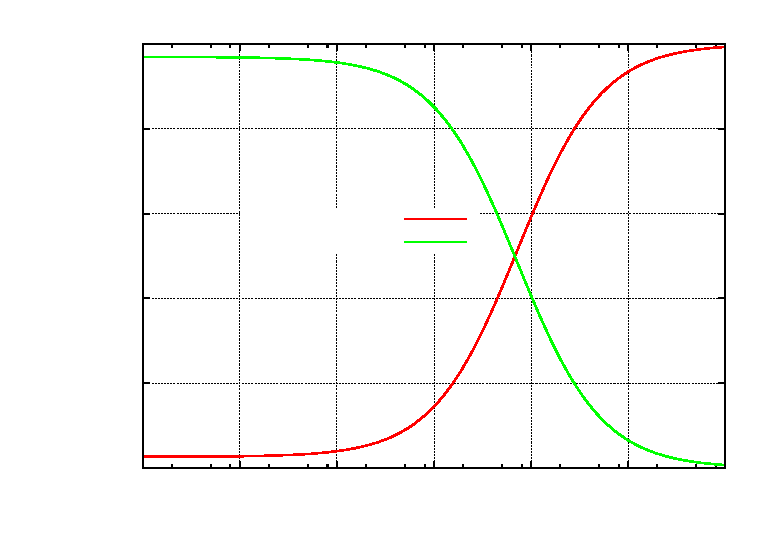
\includegraphics{../GNU/RLvtot}}%
    \gplfronttext
  \end{picture}%
\endgroup

\caption{Spannung von Type 1 und Type 2 mit Messwiderstand \(680\Omega\) }
\label{fig:RLvtot}
\end{figure}
Die Verlauf für Messung Type 1 wird in Abbildung~\ref{fig:RLvlow} mit gespreizter Darstellung für die unteren Widerstandwerte gezeigt.
Wie man sehen kann, braucht man eine bessere ADC-Auflösung als die möglichen 4,9mV bei der 5V ADC-Referenz, um richtige
Widerstandswerte von der gemessenen Spannung unter \(2\Omega\) zu erhalten.
Es gibt nur drei ADC-Stufen mit der 5V-Referenz zwischen \(0\Omega\) und \(2\Omega\).
Hier kann die Bereichsumschaltung mit der AUTOSCALE\_ADC Option helfen.
Der gleiche gespreizte Bereich für die Type 2 Messung wird in Abbildung~\ref{fig:RLvhigh} gezeigt.
Unglücklicherweise kann man nicht die höhere ADC-Auflösung für Messmethode Type 2 benutzen,
weil die Spannung zu hoch ist und unser ATmega keine differenziellen ADC-Eingänge besitzt.
Die Messungen mit den \(680\Omega\)-Widerständen werden bis zu einem Widerstandswert von 
\(20k\Omega\) (Spannung ist unter 169mV) zur Bestimmung des Messergebnisses verwendet.

Für höhere Widerstandswerte werden Messungen mit den \(470k\Omega\)-Widerständen benutzt.
Der Mittelwert von beiden Messungen wird für den angezeigten Widerstandwert benutzt, wenn alle Messungen ergeben,
dass es kein anderes Bauteil ist.
Wenn die AUTOSCALE\_ADC Funktion benutzt wird und eine der gemessenen Spannungen für beide Versionen unter 0,98V liegt,
wird ein gewichteter Mittelwert mit Faktor vier für die Messung mit der Spannung unter 0,98V benutzt. Der andere Wert wird mit Faktor eins bewertet.
Das wird wegen der Faktor vier besseren Auflösung dieser Messung gemacht.
Faktor vier wird nur für ATmega168 und ATmega328 Prozessoren verwendet, für ATmega8 wird ein
Faktor zwei als Wichtung benutzt wenn die Spannung unter 0,98V ist, weil die ADC Referenzspannung hier 2,56V statt 1,1V betr"agt.
Wenn der ATmega mehr als 8 KByte Flashspeicher besitzt, wird die Spannungsmessung an den Widerständen so lange verzögert,
bis keine \"Anderung mehr festgestellt wird oder eine Zeitgrenze überschritten wird.
Durch diese Maßnahme werden auch große Kondensatoren nicht mehr irrtümlich als
Widerstände erkannt und der Gleichstrom-Widerstand großer Induktivitäten wird richtig gemessen.

\begin{figure}[H]
  \begin{subfigure}[b]{9cm}
    \centering
    \resizebox{9cm}{!}{% GNUPLOT: LaTeX picture with Postscript
\begingroup
  \makeatletter
  \providecommand\color[2][]{%
    \GenericError{(gnuplot) \space\space\space\@spaces}{%
      Package color not loaded in conjunction with
      terminal option `colourtext'%
    }{See the gnuplot documentation for explanation.%
    }{Either use 'blacktext' in gnuplot or load the package
      color.sty in LaTeX.}%
    \renewcommand\color[2][]{}%
  }%
  \providecommand\includegraphics[2][]{%
    \GenericError{(gnuplot) \space\space\space\@spaces}{%
      Package graphicx or graphics not loaded%
    }{See the gnuplot documentation for explanation.%
    }{The gnuplot epslatex terminal needs graphicx.sty or graphics.sty.}%
    \renewcommand\includegraphics[2][]{}%
  }%
  \providecommand\rotatebox[2]{#2}%
  \@ifundefined{ifGPcolor}{%
    \newif\ifGPcolor
    \GPcolortrue
  }{}%
  \@ifundefined{ifGPblacktext}{%
    \newif\ifGPblacktext
    \GPblacktexttrue
  }{}%
  % define a \g@addto@macro without @ in the name:
  \let\gplgaddtomacro\g@addto@macro
  % define empty templates for all commands taking text:
  \gdef\gplbacktext{}%
  \gdef\gplfronttext{}%
  \makeatother
  \ifGPblacktext
    % no textcolor at all
    \def\colorrgb#1{}%
    \def\colorgray#1{}%
  \else
    % gray or color?
    \ifGPcolor
      \def\colorrgb#1{\color[rgb]{#1}}%
      \def\colorgray#1{\color[gray]{#1}}%
      \expandafter\def\csname LTw\endcsname{\color{white}}%
      \expandafter\def\csname LTb\endcsname{\color{black}}%
      \expandafter\def\csname LTa\endcsname{\color{black}}%
      \expandafter\def\csname LT0\endcsname{\color[rgb]{1,0,0}}%
      \expandafter\def\csname LT1\endcsname{\color[rgb]{0,1,0}}%
      \expandafter\def\csname LT2\endcsname{\color[rgb]{0,0,1}}%
      \expandafter\def\csname LT3\endcsname{\color[rgb]{1,0,1}}%
      \expandafter\def\csname LT4\endcsname{\color[rgb]{0,1,1}}%
      \expandafter\def\csname LT5\endcsname{\color[rgb]{1,1,0}}%
      \expandafter\def\csname LT6\endcsname{\color[rgb]{0,0,0}}%
      \expandafter\def\csname LT7\endcsname{\color[rgb]{1,0.3,0}}%
      \expandafter\def\csname LT8\endcsname{\color[rgb]{0.5,0.5,0.5}}%
    \else
      % gray
      \def\colorrgb#1{\color{black}}%
      \def\colorgray#1{\color[gray]{#1}}%
      \expandafter\def\csname LTw\endcsname{\color{white}}%
      \expandafter\def\csname LTb\endcsname{\color{black}}%
      \expandafter\def\csname LTa\endcsname{\color{black}}%
      \expandafter\def\csname LT0\endcsname{\color{black}}%
      \expandafter\def\csname LT1\endcsname{\color{black}}%
      \expandafter\def\csname LT2\endcsname{\color{black}}%
      \expandafter\def\csname LT3\endcsname{\color{black}}%
      \expandafter\def\csname LT4\endcsname{\color{black}}%
      \expandafter\def\csname LT5\endcsname{\color{black}}%
      \expandafter\def\csname LT6\endcsname{\color{black}}%
      \expandafter\def\csname LT7\endcsname{\color{black}}%
      \expandafter\def\csname LT8\endcsname{\color{black}}%
    \fi
  \fi
  \setlength{\unitlength}{0.0500bp}%
  \begin{picture}(7200.00,5040.00)%
    \gplgaddtomacro\gplbacktext{%
      \csname LTb\endcsname%
      \put(946,704){\makebox(0,0)[r]{\strut{} 130}}%
      \csname LTb\endcsname%
      \put(946,995){\makebox(0,0)[r]{\strut{} 135}}%
      \csname LTb\endcsname%
      \put(946,1286){\makebox(0,0)[r]{\strut{} 140}}%
      \csname LTb\endcsname%
      \put(946,1576){\makebox(0,0)[r]{\strut{} 145}}%
      \csname LTb\endcsname%
      \put(946,1867){\makebox(0,0)[r]{\strut{} 150}}%
      \csname LTb\endcsname%
      \put(946,2158){\makebox(0,0)[r]{\strut{} 155}}%
      \csname LTb\endcsname%
      \put(946,2449){\makebox(0,0)[r]{\strut{} 160}}%
      \csname LTb\endcsname%
      \put(946,2740){\makebox(0,0)[r]{\strut{} 165}}%
      \csname LTb\endcsname%
      \put(946,3030){\makebox(0,0)[r]{\strut{} 170}}%
      \csname LTb\endcsname%
      \put(946,3321){\makebox(0,0)[r]{\strut{} 175}}%
      \csname LTb\endcsname%
      \put(946,3612){\makebox(0,0)[r]{\strut{} 180}}%
      \csname LTb\endcsname%
      \put(946,3903){\makebox(0,0)[r]{\strut{} 185}}%
      \csname LTb\endcsname%
      \put(946,4193){\makebox(0,0)[r]{\strut{} 190}}%
      \csname LTb\endcsname%
      \put(946,4484){\makebox(0,0)[r]{\strut{} 195}}%
      \csname LTb\endcsname%
      \put(946,4775){\makebox(0,0)[r]{\strut{} 200}}%
      \csname LTb\endcsname%
      \put(1078,484){\makebox(0,0){\strut{} 0}}%
      \csname LTb\endcsname%
      \put(1651,484){\makebox(0,0){\strut{} 1}}%
      \csname LTb\endcsname%
      \put(2223,484){\makebox(0,0){\strut{} 2}}%
      \csname LTb\endcsname%
      \put(2796,484){\makebox(0,0){\strut{} 3}}%
      \csname LTb\endcsname%
      \put(3368,484){\makebox(0,0){\strut{} 4}}%
      \csname LTb\endcsname%
      \put(3941,484){\makebox(0,0){\strut{} 5}}%
      \csname LTb\endcsname%
      \put(4513,484){\makebox(0,0){\strut{} 6}}%
      \csname LTb\endcsname%
      \put(5086,484){\makebox(0,0){\strut{} 7}}%
      \csname LTb\endcsname%
      \put(5658,484){\makebox(0,0){\strut{} 8}}%
      \csname LTb\endcsname%
      \put(6231,484){\makebox(0,0){\strut{} 9}}%
      \csname LTb\endcsname%
      \put(6803,484){\makebox(0,0){\strut{} 10}}%
      \put(176,2739){\rotatebox{-270}{\makebox(0,0){\strut{}voltage / mV}}}%
      \put(3940,154){\makebox(0,0){\strut{}resistor Rx / Ohm}}%
      \put(3940,4665){\makebox(0,0){\strut{}}}%
    }%
    \gplgaddtomacro\gplfronttext{%
      \csname LTb\endcsname%
      \put(5816,4602){\makebox(0,0)[r]{\strut{}PC2, type 1}}%
    }%
    \gplbacktext
    \put(0,0){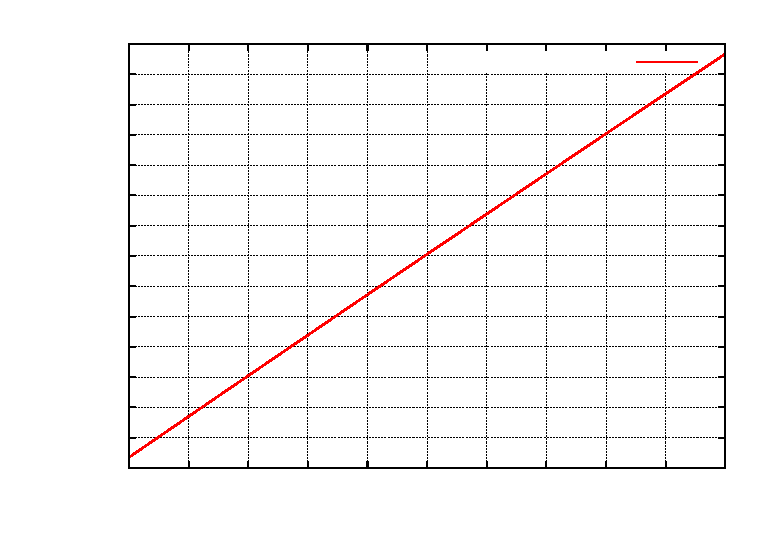
\includegraphics{../GNU/RLvlow}}%
    \gplfronttext
  \end{picture}%
\endgroup
}
    \caption{Type 1 Messung}
    \label{fig:RLvlow}
  \end{subfigure}
  ~
  \begin{subfigure}[b]{9cm}
    \centering
    \resizebox{9cm}{!}{% GNUPLOT: LaTeX picture with Postscript
\begingroup
  \makeatletter
  \providecommand\color[2][]{%
    \GenericError{(gnuplot) \space\space\space\@spaces}{%
      Package color not loaded in conjunction with
      terminal option `colourtext'%
    }{See the gnuplot documentation for explanation.%
    }{Either use 'blacktext' in gnuplot or load the package
      color.sty in LaTeX.}%
    \renewcommand\color[2][]{}%
  }%
  \providecommand\includegraphics[2][]{%
    \GenericError{(gnuplot) \space\space\space\@spaces}{%
      Package graphicx or graphics not loaded%
    }{See the gnuplot documentation for explanation.%
    }{The gnuplot epslatex terminal needs graphicx.sty or graphics.sty.}%
    \renewcommand\includegraphics[2][]{}%
  }%
  \providecommand\rotatebox[2]{#2}%
  \@ifundefined{ifGPcolor}{%
    \newif\ifGPcolor
    \GPcolortrue
  }{}%
  \@ifundefined{ifGPblacktext}{%
    \newif\ifGPblacktext
    \GPblacktexttrue
  }{}%
  % define a \g@addto@macro without @ in the name:
  \let\gplgaddtomacro\g@addto@macro
  % define empty templates for all commands taking text:
  \gdef\gplbacktext{}%
  \gdef\gplfronttext{}%
  \makeatother
  \ifGPblacktext
    % no textcolor at all
    \def\colorrgb#1{}%
    \def\colorgray#1{}%
  \else
    % gray or color?
    \ifGPcolor
      \def\colorrgb#1{\color[rgb]{#1}}%
      \def\colorgray#1{\color[gray]{#1}}%
      \expandafter\def\csname LTw\endcsname{\color{white}}%
      \expandafter\def\csname LTb\endcsname{\color{black}}%
      \expandafter\def\csname LTa\endcsname{\color{black}}%
      \expandafter\def\csname LT0\endcsname{\color[rgb]{1,0,0}}%
      \expandafter\def\csname LT1\endcsname{\color[rgb]{0,1,0}}%
      \expandafter\def\csname LT2\endcsname{\color[rgb]{0,0,1}}%
      \expandafter\def\csname LT3\endcsname{\color[rgb]{1,0,1}}%
      \expandafter\def\csname LT4\endcsname{\color[rgb]{0,1,1}}%
      \expandafter\def\csname LT5\endcsname{\color[rgb]{1,1,0}}%
      \expandafter\def\csname LT6\endcsname{\color[rgb]{0,0,0}}%
      \expandafter\def\csname LT7\endcsname{\color[rgb]{1,0.3,0}}%
      \expandafter\def\csname LT8\endcsname{\color[rgb]{0.5,0.5,0.5}}%
    \else
      % gray
      \def\colorrgb#1{\color{black}}%
      \def\colorgray#1{\color[gray]{#1}}%
      \expandafter\def\csname LTw\endcsname{\color{white}}%
      \expandafter\def\csname LTb\endcsname{\color{black}}%
      \expandafter\def\csname LTa\endcsname{\color{black}}%
      \expandafter\def\csname LT0\endcsname{\color{black}}%
      \expandafter\def\csname LT1\endcsname{\color{black}}%
      \expandafter\def\csname LT2\endcsname{\color{black}}%
      \expandafter\def\csname LT3\endcsname{\color{black}}%
      \expandafter\def\csname LT4\endcsname{\color{black}}%
      \expandafter\def\csname LT5\endcsname{\color{black}}%
      \expandafter\def\csname LT6\endcsname{\color{black}}%
      \expandafter\def\csname LT7\endcsname{\color{black}}%
      \expandafter\def\csname LT8\endcsname{\color{black}}%
    \fi
  \fi
  \setlength{\unitlength}{0.0500bp}%
  \begin{picture}(7200.00,5040.00)%
    \gplgaddtomacro\gplbacktext{%
      \csname LTb\endcsname%
      \put(1078,704){\makebox(0,0)[r]{\strut{} 4780}}%
      \csname LTb\endcsname%
      \put(1078,995){\makebox(0,0)[r]{\strut{} 4785}}%
      \csname LTb\endcsname%
      \put(1078,1286){\makebox(0,0)[r]{\strut{} 4790}}%
      \csname LTb\endcsname%
      \put(1078,1576){\makebox(0,0)[r]{\strut{} 4795}}%
      \csname LTb\endcsname%
      \put(1078,1867){\makebox(0,0)[r]{\strut{} 4800}}%
      \csname LTb\endcsname%
      \put(1078,2158){\makebox(0,0)[r]{\strut{} 4805}}%
      \csname LTb\endcsname%
      \put(1078,2449){\makebox(0,0)[r]{\strut{} 4810}}%
      \csname LTb\endcsname%
      \put(1078,2740){\makebox(0,0)[r]{\strut{} 4815}}%
      \csname LTb\endcsname%
      \put(1078,3030){\makebox(0,0)[r]{\strut{} 4820}}%
      \csname LTb\endcsname%
      \put(1078,3321){\makebox(0,0)[r]{\strut{} 4825}}%
      \csname LTb\endcsname%
      \put(1078,3612){\makebox(0,0)[r]{\strut{} 4830}}%
      \csname LTb\endcsname%
      \put(1078,3903){\makebox(0,0)[r]{\strut{} 4835}}%
      \csname LTb\endcsname%
      \put(1078,4193){\makebox(0,0)[r]{\strut{} 4840}}%
      \csname LTb\endcsname%
      \put(1078,4484){\makebox(0,0)[r]{\strut{} 4845}}%
      \csname LTb\endcsname%
      \put(1078,4775){\makebox(0,0)[r]{\strut{} 4850}}%
      \csname LTb\endcsname%
      \put(1210,484){\makebox(0,0){\strut{} 0}}%
      \csname LTb\endcsname%
      \put(1769,484){\makebox(0,0){\strut{} 1}}%
      \csname LTb\endcsname%
      \put(2329,484){\makebox(0,0){\strut{} 2}}%
      \csname LTb\endcsname%
      \put(2888,484){\makebox(0,0){\strut{} 3}}%
      \csname LTb\endcsname%
      \put(3447,484){\makebox(0,0){\strut{} 4}}%
      \csname LTb\endcsname%
      \put(4007,484){\makebox(0,0){\strut{} 5}}%
      \csname LTb\endcsname%
      \put(4566,484){\makebox(0,0){\strut{} 6}}%
      \csname LTb\endcsname%
      \put(5125,484){\makebox(0,0){\strut{} 7}}%
      \csname LTb\endcsname%
      \put(5684,484){\makebox(0,0){\strut{} 8}}%
      \csname LTb\endcsname%
      \put(6244,484){\makebox(0,0){\strut{} 9}}%
      \csname LTb\endcsname%
      \put(6803,484){\makebox(0,0){\strut{} 10}}%
      \put(176,2739){\rotatebox{-270}{\makebox(0,0){\strut{}voltage / mV}}}%
      \put(4006,154){\makebox(0,0){\strut{}resistor Rx / Ohm}}%
      \put(4006,4665){\makebox(0,0){\strut{}}}%
      \put(286,110){\makebox(0,0)[l]{\strut{}}}%
    }%
    \gplgaddtomacro\gplfronttext{%
      \csname LTb\endcsname%
      \put(5816,4602){\makebox(0,0)[r]{\strut{}PC0, type 2}}%
    }%
    \gplbacktext
    \put(0,0){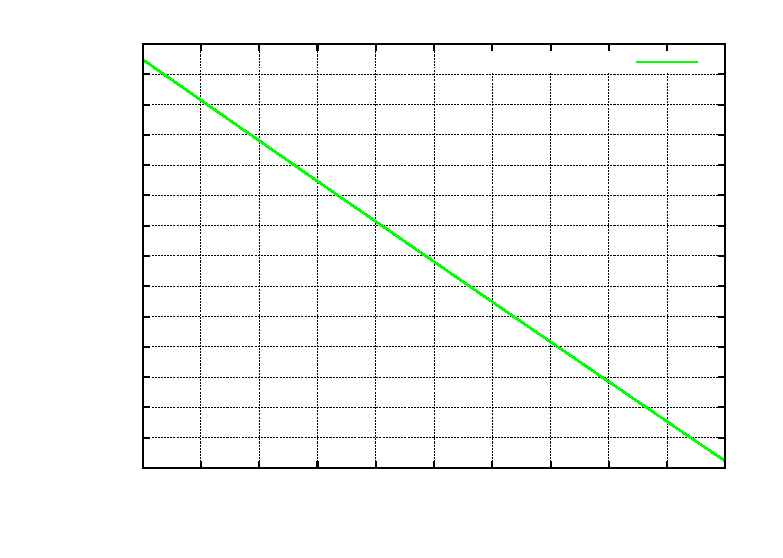
\includegraphics{../GNU/RLvhigh}}%
    \gplfronttext
  \end{picture}%
\endgroup
}
    \caption{Type 2 Messung}
    \label{fig:RLvhigh}
  \end{subfigure}
  \caption{Ausschnitt des theoretischen Spannungsverlauf von \(0\Omega\) bis \(10\Omega\)}
\end{figure}


\subsection{Widerstandsmessung mit den 470-kOhm-Widerständen}
Die nächsten Abbildungen~\ref{fig:RH1mes} und \ref{fig:RH2mes} zeigen die gleichen Messmethoden für die Messungen mit
 \(470k\Omega\)-Präzisionswiderständen.
Weil \(470k\Omega\) in Relation zu den Port-Widerständen \(22\Omega\) und \(19\Omega\) sehr groß ist ,
können die Port-Widerstände für die Berechnung des Widerstandswertes Rx vernachlässigt werden.

Für beide Messmethoden mit den \(470k\Omega\)-Widerständen wird nur eine Spannung gemessen, weil der Strom
so niedrig ist, dass keine Spannungsdifferenz an den internen Port Widerständen gemessen werden kann (wie zu erwarten).
Der theoretische Spannungsverlauf wird in Abbildung~\ref{fig:RHv} gezeigt, wobei die Widerstandswerte wieder in
logarithmischer Skalierung gezeigt werden.
Der theoretische Verlauf in diesem Diagramm endet bei \(100M\Omega\), aber das Ergebnis des Testers wird auf
 \(60M\Omega\) begrenzt, anderenfalls nimmt der Tester an, dass kein Widerstand angeschlossen ist.
Als Ergebnis wird der gewichtete Mittelwert von beiden Messmethoden verwendet. Dies geschieht nach den gleichen Regeln, die schon bei
den Messungen mit den  \(680\Omega\) Widerständen beschrieben wurden.
Ich habe beobachtet, dass die Messergebnisse für alle ATmega Typen  näher am wahren Wert liegen, wenn zum Messergebnis
ein konstanter Offset von \(350\Omega\) addiert wird.
Dieser Offset kann mit der Konstante RH\_OFFSET (define) in der Datei config.h angepasst werden.

\begin{figure}[H]
\centering

\includegraphics[]{../FIG/ResistormessH1.eps}
\caption{Messung Type 3 mit \(470k\Omega\) }
\label{fig:RH1mes}
\end{figure}

\begin{figure}[H]
 \centering
 
\includegraphics[]{../FIG/ResistormessH2.eps}
 \caption{Messung Type 4 mit \(470k\Omega\) }
\label{fig:RH2mes}
\end{figure}

\begin{figure}[H]
\centering
% GNUPLOT: LaTeX picture with Postscript
\begingroup
  \makeatletter
  \providecommand\color[2][]{%
    \GenericError{(gnuplot) \space\space\space\@spaces}{%
      Package color not loaded in conjunction with
      terminal option `colourtext'%
    }{See the gnuplot documentation for explanation.%
    }{Either use 'blacktext' in gnuplot or load the package
      color.sty in LaTeX.}%
    \renewcommand\color[2][]{}%
  }%
  \providecommand\includegraphics[2][]{%
    \GenericError{(gnuplot) \space\space\space\@spaces}{%
      Package graphicx or graphics not loaded%
    }{See the gnuplot documentation for explanation.%
    }{The gnuplot epslatex terminal needs graphicx.sty or graphics.sty.}%
    \renewcommand\includegraphics[2][]{}%
  }%
  \providecommand\rotatebox[2]{#2}%
  \@ifundefined{ifGPcolor}{%
    \newif\ifGPcolor
    \GPcolortrue
  }{}%
  \@ifundefined{ifGPblacktext}{%
    \newif\ifGPblacktext
    \GPblacktexttrue
  }{}%
  % define a \g@addto@macro without @ in the name:
  \let\gplgaddtomacro\g@addto@macro
  % define empty templates for all commands taking text:
  \gdef\gplbacktext{}%
  \gdef\gplfronttext{}%
  \makeatother
  \ifGPblacktext
    % no textcolor at all
    \def\colorrgb#1{}%
    \def\colorgray#1{}%
  \else
    % gray or color?
    \ifGPcolor
      \def\colorrgb#1{\color[rgb]{#1}}%
      \def\colorgray#1{\color[gray]{#1}}%
      \expandafter\def\csname LTw\endcsname{\color{white}}%
      \expandafter\def\csname LTb\endcsname{\color{black}}%
      \expandafter\def\csname LTa\endcsname{\color{black}}%
      \expandafter\def\csname LT0\endcsname{\color[rgb]{1,0,0}}%
      \expandafter\def\csname LT1\endcsname{\color[rgb]{0,1,0}}%
      \expandafter\def\csname LT2\endcsname{\color[rgb]{0,0,1}}%
      \expandafter\def\csname LT3\endcsname{\color[rgb]{1,0,1}}%
      \expandafter\def\csname LT4\endcsname{\color[rgb]{0,1,1}}%
      \expandafter\def\csname LT5\endcsname{\color[rgb]{1,1,0}}%
      \expandafter\def\csname LT6\endcsname{\color[rgb]{0,0,0}}%
      \expandafter\def\csname LT7\endcsname{\color[rgb]{1,0.3,0}}%
      \expandafter\def\csname LT8\endcsname{\color[rgb]{0.5,0.5,0.5}}%
    \else
      % gray
      \def\colorrgb#1{\color{black}}%
      \def\colorgray#1{\color[gray]{#1}}%
      \expandafter\def\csname LTw\endcsname{\color{white}}%
      \expandafter\def\csname LTb\endcsname{\color{black}}%
      \expandafter\def\csname LTa\endcsname{\color{black}}%
      \expandafter\def\csname LT0\endcsname{\color{black}}%
      \expandafter\def\csname LT1\endcsname{\color{black}}%
      \expandafter\def\csname LT2\endcsname{\color{black}}%
      \expandafter\def\csname LT3\endcsname{\color{black}}%
      \expandafter\def\csname LT4\endcsname{\color{black}}%
      \expandafter\def\csname LT5\endcsname{\color{black}}%
      \expandafter\def\csname LT6\endcsname{\color{black}}%
      \expandafter\def\csname LT7\endcsname{\color{black}}%
      \expandafter\def\csname LT8\endcsname{\color{black}}%
    \fi
  \fi
  \setlength{\unitlength}{0.0500bp}%
  \begin{picture}(7200.00,5040.00)%
    \gplgaddtomacro\gplbacktext{%
      \csname LTb\endcsname%
      \put(1078,704){\makebox(0,0)[r]{\strut{} 0}}%
      \csname LTb\endcsname%
      \put(1078,1518){\makebox(0,0)[r]{\strut{} 1000}}%
      \csname LTb\endcsname%
      \put(1078,2332){\makebox(0,0)[r]{\strut{} 2000}}%
      \csname LTb\endcsname%
      \put(1078,3147){\makebox(0,0)[r]{\strut{} 3000}}%
      \csname LTb\endcsname%
      \put(1078,3961){\makebox(0,0)[r]{\strut{} 4000}}%
      \csname LTb\endcsname%
      \put(1078,4775){\makebox(0,0)[r]{\strut{} 5000}}%
      \csname LTb\endcsname%
      \put(1210,484){\makebox(0,0){\strut{}10k}}%
      \csname LTb\endcsname%
      \put(2608,484){\makebox(0,0){\strut{}100k}}%
      \csname LTb\endcsname%
      \put(4007,484){\makebox(0,0){\strut{}1M}}%
      \csname LTb\endcsname%
      \put(5405,484){\makebox(0,0){\strut{}10M}}%
      \csname LTb\endcsname%
      \put(6803,484){\makebox(0,0){\strut{}100M}}%
      \put(176,2739){\rotatebox{-270}{\makebox(0,0){\strut{}voltage / mV}}}%
      \put(4006,154){\makebox(0,0){\strut{}resistor Rx / Ohm}}%
      \put(4006,4665){\makebox(0,0){\strut{}}}%
    }%
    \gplgaddtomacro\gplfronttext{%
      \csname LTb\endcsname%
      \put(5948,2874){\makebox(0,0)[r]{\strut{}PC2 type 3}}%
      \csname LTb\endcsname%
      \put(5948,2654){\makebox(0,0)[r]{\strut{}PC0, type 4}}%
    }%
    \gplbacktext
    \put(0,0){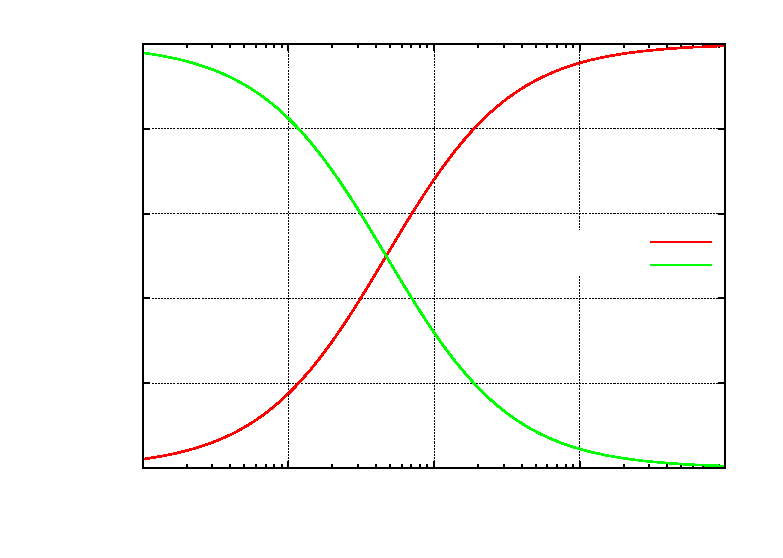
\includegraphics{../GNU/RHv}}%
    \gplfronttext
  \end{picture}%
\endgroup

\caption{Spannungen bei Messungen von Type 3 und Type 4  mit \(470k\Omega\) }
\label{fig:RHv}
\end{figure}

\subsection{Ergebnisse der Widerstands-Messung}
Abbildung~\ref{fig:mega8res} zeigt den relativen Fehler der Widerstandmessung mit drei verschiedenen ATmega8. 
Zusätzlich werden die Meßergebnisse einiger Widerstände mit der Originalsoftware von Markus F. als
,,Mega8orig'' gezeigt.
Die Meßergebnisse der gleichen Widerstände mit je drei ATmega8A und drei ATmega8L werden in den Abbildungen
\ref{fig:mega8Ares} und \ref{fig:mega8Lres} gezeigt.
Abbildung~\ref{fig:mega168res} zeigt die gleichen Messungen mit einem ATmega168.
,,Mega168'' sind die Ergebnisse ohne die AUTOSCALE\_ADC Option, ,,Mega168as'' die mit der
 AUTOSCALE\_ADC Option.

Mit dem ATmega168 scheint es möglich zu sein, Messungen von Widerständen im
Bereich von \(20\Omega\) bis \(20M\Omega\) mit einem Messfehler von unter \(\pm1\%\) durchzuführen.
Für Messungen unterhalb von \(100\Omega\) sollte man berücksichtigen, dass jede Prüfklemme mit Kabel ebenfalls
einen Widerstandwert hat.
Es ist besser, den Widerstand direkt mit den Anschlussklemmen zu verbinden.
Wenn das nicht möglich ist, sollte man der Widerstandswert der kurzgeschlossenen Prüfklemmen vom Messergebnis abziehen.
Zeigt beispielsweise der Tester einen Wert von \(30,6\Omega\) an, wenn der Präzisionswiderstand einen aufgedruckten Wert von \(30\Omega\) hat, 
und die im Kurzschluss gemessenen Prüfklemmen haben einen Wert von \(0,5\Omega\), dann wird der Widerstand vom
Tester mit \(30,1\Omega\) gemessen.
Unterhalb von einem Widerstandswert von \(10\Omega\) macht ein Auflösungs-Schritt von \(0,1\Omega\) schon einen Fehler von mehr als 1\%!

\begin{figure}[H]
\centering
% GNUPLOT: LaTeX picture with Postscript
\begingroup
  \makeatletter
  \providecommand\color[2][]{%
    \GenericError{(gnuplot) \space\space\space\@spaces}{%
      Package color not loaded in conjunction with
      terminal option `colourtext'%
    }{See the gnuplot documentation for explanation.%
    }{Either use 'blacktext' in gnuplot or load the package
      color.sty in LaTeX.}%
    \renewcommand\color[2][]{}%
  }%
  \providecommand\includegraphics[2][]{%
    \GenericError{(gnuplot) \space\space\space\@spaces}{%
      Package graphicx or graphics not loaded%
    }{See the gnuplot documentation for explanation.%
    }{The gnuplot epslatex terminal needs graphicx.sty or graphics.sty.}%
    \renewcommand\includegraphics[2][]{}%
  }%
  \providecommand\rotatebox[2]{#2}%
  \@ifundefined{ifGPcolor}{%
    \newif\ifGPcolor
    \GPcolortrue
  }{}%
  \@ifundefined{ifGPblacktext}{%
    \newif\ifGPblacktext
    \GPblacktexttrue
  }{}%
  % define a \g@addto@macro without @ in the name:
  \let\gplgaddtomacro\g@addto@macro
  % define empty templates for all commands taking text:
  \gdef\gplbacktext{}%
  \gdef\gplfronttext{}%
  \makeatother
  \ifGPblacktext
    % no textcolor at all
    \def\colorrgb#1{}%
    \def\colorgray#1{}%
  \else
    % gray or color?
    \ifGPcolor
      \def\colorrgb#1{\color[rgb]{#1}}%
      \def\colorgray#1{\color[gray]{#1}}%
      \expandafter\def\csname LTw\endcsname{\color{white}}%
      \expandafter\def\csname LTb\endcsname{\color{black}}%
      \expandafter\def\csname LTa\endcsname{\color{black}}%
      \expandafter\def\csname LT0\endcsname{\color[rgb]{1,0,0}}%
      \expandafter\def\csname LT1\endcsname{\color[rgb]{0,1,0}}%
      \expandafter\def\csname LT2\endcsname{\color[rgb]{0,0,1}}%
      \expandafter\def\csname LT3\endcsname{\color[rgb]{1,0,1}}%
      \expandafter\def\csname LT4\endcsname{\color[rgb]{0,1,1}}%
      \expandafter\def\csname LT5\endcsname{\color[rgb]{1,1,0}}%
      \expandafter\def\csname LT6\endcsname{\color[rgb]{0,0,0}}%
      \expandafter\def\csname LT7\endcsname{\color[rgb]{1,0.3,0}}%
      \expandafter\def\csname LT8\endcsname{\color[rgb]{0.5,0.5,0.5}}%
    \else
      % gray
      \def\colorrgb#1{\color{black}}%
      \def\colorgray#1{\color[gray]{#1}}%
      \expandafter\def\csname LTw\endcsname{\color{white}}%
      \expandafter\def\csname LTb\endcsname{\color{black}}%
      \expandafter\def\csname LTa\endcsname{\color{black}}%
      \expandafter\def\csname LT0\endcsname{\color{black}}%
      \expandafter\def\csname LT1\endcsname{\color{black}}%
      \expandafter\def\csname LT2\endcsname{\color{black}}%
      \expandafter\def\csname LT3\endcsname{\color{black}}%
      \expandafter\def\csname LT4\endcsname{\color{black}}%
      \expandafter\def\csname LT5\endcsname{\color{black}}%
      \expandafter\def\csname LT6\endcsname{\color{black}}%
      \expandafter\def\csname LT7\endcsname{\color{black}}%
      \expandafter\def\csname LT8\endcsname{\color{black}}%
    \fi
  \fi
  \setlength{\unitlength}{0.0500bp}%
  \begin{picture}(7200.00,5040.00)%
    \gplgaddtomacro\gplbacktext{%
      \csname LTb\endcsname%
      \put(682,704){\makebox(0,0)[r]{\strut{}-5}}%
      \csname LTb\endcsname%
      \put(682,1111){\makebox(0,0)[r]{\strut{}-4}}%
      \csname LTb\endcsname%
      \put(682,1518){\makebox(0,0)[r]{\strut{}-3}}%
      \csname LTb\endcsname%
      \put(682,1925){\makebox(0,0)[r]{\strut{}-2}}%
      \csname LTb\endcsname%
      \put(682,2332){\makebox(0,0)[r]{\strut{}-1}}%
      \csname LTb\endcsname%
      \put(682,2740){\makebox(0,0)[r]{\strut{} 0}}%
      \csname LTb\endcsname%
      \put(682,3147){\makebox(0,0)[r]{\strut{} 1}}%
      \csname LTb\endcsname%
      \put(682,3554){\makebox(0,0)[r]{\strut{} 2}}%
      \csname LTb\endcsname%
      \put(682,3961){\makebox(0,0)[r]{\strut{} 3}}%
      \csname LTb\endcsname%
      \put(682,4368){\makebox(0,0)[r]{\strut{} 4}}%
      \csname LTb\endcsname%
      \put(682,4775){\makebox(0,0)[r]{\strut{} 5}}%
      \csname LTb\endcsname%
      \put(814,484){\makebox(0,0){\strut{}1 }}%
      \csname LTb\endcsname%
      \put(1563,484){\makebox(0,0){\strut{}10 }}%
      \csname LTb\endcsname%
      \put(2311,484){\makebox(0,0){\strut{}100 }}%
      \csname LTb\endcsname%
      \put(3060,484){\makebox(0,0){\strut{}1k}}%
      \csname LTb\endcsname%
      \put(3809,484){\makebox(0,0){\strut{}10k}}%
      \csname LTb\endcsname%
      \put(4557,484){\makebox(0,0){\strut{}100k}}%
      \csname LTb\endcsname%
      \put(5306,484){\makebox(0,0){\strut{}1M}}%
      \csname LTb\endcsname%
      \put(6054,484){\makebox(0,0){\strut{}10M}}%
      \csname LTb\endcsname%
      \put(6803,484){\makebox(0,0){\strut{}100M}}%
      \put(176,2739){\rotatebox{-270}{\makebox(0,0){\strut{}Error / Percent}}}%
      \put(3808,154){\makebox(0,0){\strut{}Resistor value / Ohm}}%
    }%
    \gplgaddtomacro\gplfronttext{%
      \csname LTb\endcsname%
      \put(5753,4602){\makebox(0,0)[r]{\strut{}Mega8-1}}%
      \csname LTb\endcsname%
      \put(5753,4382){\makebox(0,0)[r]{\strut{}Mega8-2}}%
      \csname LTb\endcsname%
      \put(5753,4162){\makebox(0,0)[r]{\strut{}Mega8-3}}%
      \csname LTb\endcsname%
      \put(5753,3942){\makebox(0,0)[r]{\strut{}Mega8orig}}%
    }%
    \gplbacktext
    \put(0,0){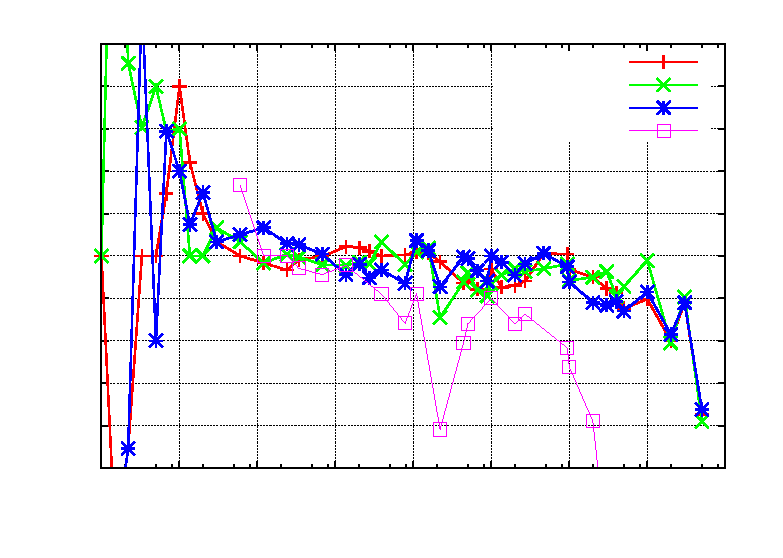
\includegraphics{../GNU/Mega8res}}%
    \gplfronttext
  \end{picture}%
\endgroup

\caption{Relativer Fehler für Widerstands-Messungen mit ATmega8 }
\label{fig:mega8res}
\end{figure}

\begin{figure}[H]
  \begin{subfigure}[b]{9cm}
    \centering
    \resizebox{9cm}{!}{% GNUPLOT: LaTeX picture with Postscript
\begingroup
  \makeatletter
  \providecommand\color[2][]{%
    \GenericError{(gnuplot) \space\space\space\@spaces}{%
      Package color not loaded in conjunction with
      terminal option `colourtext'%
    }{See the gnuplot documentation for explanation.%
    }{Either use 'blacktext' in gnuplot or load the package
      color.sty in LaTeX.}%
    \renewcommand\color[2][]{}%
  }%
  \providecommand\includegraphics[2][]{%
    \GenericError{(gnuplot) \space\space\space\@spaces}{%
      Package graphicx or graphics not loaded%
    }{See the gnuplot documentation for explanation.%
    }{The gnuplot epslatex terminal needs graphicx.sty or graphics.sty.}%
    \renewcommand\includegraphics[2][]{}%
  }%
  \providecommand\rotatebox[2]{#2}%
  \@ifundefined{ifGPcolor}{%
    \newif\ifGPcolor
    \GPcolortrue
  }{}%
  \@ifundefined{ifGPblacktext}{%
    \newif\ifGPblacktext
    \GPblacktexttrue
  }{}%
  % define a \g@addto@macro without @ in the name:
  \let\gplgaddtomacro\g@addto@macro
  % define empty templates for all commands taking text:
  \gdef\gplbacktext{}%
  \gdef\gplfronttext{}%
  \makeatother
  \ifGPblacktext
    % no textcolor at all
    \def\colorrgb#1{}%
    \def\colorgray#1{}%
  \else
    % gray or color?
    \ifGPcolor
      \def\colorrgb#1{\color[rgb]{#1}}%
      \def\colorgray#1{\color[gray]{#1}}%
      \expandafter\def\csname LTw\endcsname{\color{white}}%
      \expandafter\def\csname LTb\endcsname{\color{black}}%
      \expandafter\def\csname LTa\endcsname{\color{black}}%
      \expandafter\def\csname LT0\endcsname{\color[rgb]{1,0,0}}%
      \expandafter\def\csname LT1\endcsname{\color[rgb]{0,1,0}}%
      \expandafter\def\csname LT2\endcsname{\color[rgb]{0,0,1}}%
      \expandafter\def\csname LT3\endcsname{\color[rgb]{1,0,1}}%
      \expandafter\def\csname LT4\endcsname{\color[rgb]{0,1,1}}%
      \expandafter\def\csname LT5\endcsname{\color[rgb]{1,1,0}}%
      \expandafter\def\csname LT6\endcsname{\color[rgb]{0,0,0}}%
      \expandafter\def\csname LT7\endcsname{\color[rgb]{1,0.3,0}}%
      \expandafter\def\csname LT8\endcsname{\color[rgb]{0.5,0.5,0.5}}%
    \else
      % gray
      \def\colorrgb#1{\color{black}}%
      \def\colorgray#1{\color[gray]{#1}}%
      \expandafter\def\csname LTw\endcsname{\color{white}}%
      \expandafter\def\csname LTb\endcsname{\color{black}}%
      \expandafter\def\csname LTa\endcsname{\color{black}}%
      \expandafter\def\csname LT0\endcsname{\color{black}}%
      \expandafter\def\csname LT1\endcsname{\color{black}}%
      \expandafter\def\csname LT2\endcsname{\color{black}}%
      \expandafter\def\csname LT3\endcsname{\color{black}}%
      \expandafter\def\csname LT4\endcsname{\color{black}}%
      \expandafter\def\csname LT5\endcsname{\color{black}}%
      \expandafter\def\csname LT6\endcsname{\color{black}}%
      \expandafter\def\csname LT7\endcsname{\color{black}}%
      \expandafter\def\csname LT8\endcsname{\color{black}}%
    \fi
  \fi
  \setlength{\unitlength}{0.0500bp}%
  \begin{picture}(7200.00,5040.00)%
    \gplgaddtomacro\gplbacktext{%
      \csname LTb\endcsname%
      \put(682,704){\makebox(0,0)[r]{\strut{}-5}}%
      \csname LTb\endcsname%
      \put(682,1111){\makebox(0,0)[r]{\strut{}-4}}%
      \csname LTb\endcsname%
      \put(682,1518){\makebox(0,0)[r]{\strut{}-3}}%
      \csname LTb\endcsname%
      \put(682,1925){\makebox(0,0)[r]{\strut{}-2}}%
      \csname LTb\endcsname%
      \put(682,2332){\makebox(0,0)[r]{\strut{}-1}}%
      \csname LTb\endcsname%
      \put(682,2740){\makebox(0,0)[r]{\strut{} 0}}%
      \csname LTb\endcsname%
      \put(682,3147){\makebox(0,0)[r]{\strut{} 1}}%
      \csname LTb\endcsname%
      \put(682,3554){\makebox(0,0)[r]{\strut{} 2}}%
      \csname LTb\endcsname%
      \put(682,3961){\makebox(0,0)[r]{\strut{} 3}}%
      \csname LTb\endcsname%
      \put(682,4368){\makebox(0,0)[r]{\strut{} 4}}%
      \csname LTb\endcsname%
      \put(682,4775){\makebox(0,0)[r]{\strut{} 5}}%
      \csname LTb\endcsname%
      \put(814,484){\makebox(0,0){\strut{}1 }}%
      \csname LTb\endcsname%
      \put(1563,484){\makebox(0,0){\strut{}10 }}%
      \csname LTb\endcsname%
      \put(2311,484){\makebox(0,0){\strut{}100 }}%
      \csname LTb\endcsname%
      \put(3060,484){\makebox(0,0){\strut{}1k}}%
      \csname LTb\endcsname%
      \put(3809,484){\makebox(0,0){\strut{}10k}}%
      \csname LTb\endcsname%
      \put(4557,484){\makebox(0,0){\strut{}100k}}%
      \csname LTb\endcsname%
      \put(5306,484){\makebox(0,0){\strut{}1M}}%
      \csname LTb\endcsname%
      \put(6054,484){\makebox(0,0){\strut{}10M}}%
      \csname LTb\endcsname%
      \put(6803,484){\makebox(0,0){\strut{}100M}}%
      \put(176,2739){\rotatebox{-270}{\makebox(0,0){\strut{}Error / Percent}}}%
      \put(3808,154){\makebox(0,0){\strut{}Resistor value / Ohm}}%
    }%
    \gplgaddtomacro\gplfronttext{%
      \csname LTb\endcsname%
      \put(5753,4602){\makebox(0,0)[r]{\strut{}Mega8A-4}}%
      \csname LTb\endcsname%
      \put(5753,4382){\makebox(0,0)[r]{\strut{}Mega8A-5}}%
      \csname LTb\endcsname%
      \put(5753,4162){\makebox(0,0)[r]{\strut{}Mega8A-6}}%
    }%
    \gplbacktext
    \put(0,0){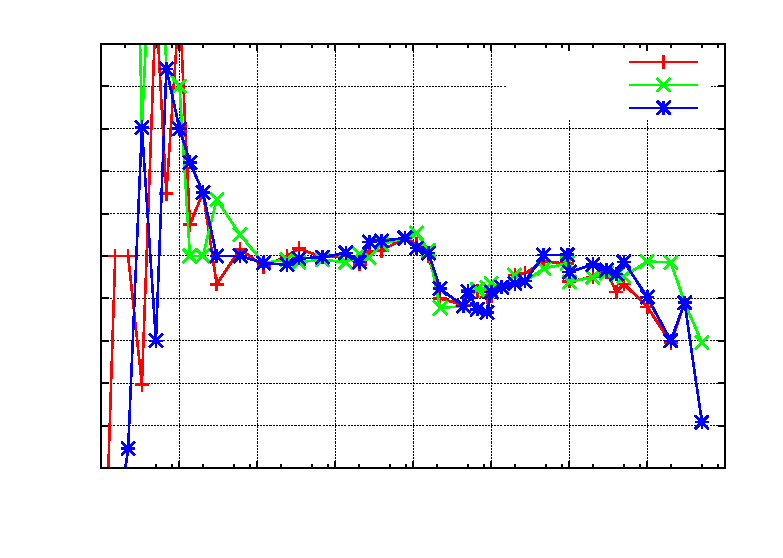
\includegraphics{../GNU/Mega8Ares}}%
    \gplfronttext
  \end{picture}%
\endgroup
}
    \caption{mit drei ATmega8A}
    \label{fig:mega8Ares}
  \end{subfigure}
  ~
  \begin{subfigure}[b]{9cm}
    \centering
    \resizebox{9cm}{!}{% GNUPLOT: LaTeX picture with Postscript
\begingroup
  \makeatletter
  \providecommand\color[2][]{%
    \GenericError{(gnuplot) \space\space\space\@spaces}{%
      Package color not loaded in conjunction with
      terminal option `colourtext'%
    }{See the gnuplot documentation for explanation.%
    }{Either use 'blacktext' in gnuplot or load the package
      color.sty in LaTeX.}%
    \renewcommand\color[2][]{}%
  }%
  \providecommand\includegraphics[2][]{%
    \GenericError{(gnuplot) \space\space\space\@spaces}{%
      Package graphicx or graphics not loaded%
    }{See the gnuplot documentation for explanation.%
    }{The gnuplot epslatex terminal needs graphicx.sty or graphics.sty.}%
    \renewcommand\includegraphics[2][]{}%
  }%
  \providecommand\rotatebox[2]{#2}%
  \@ifundefined{ifGPcolor}{%
    \newif\ifGPcolor
    \GPcolortrue
  }{}%
  \@ifundefined{ifGPblacktext}{%
    \newif\ifGPblacktext
    \GPblacktexttrue
  }{}%
  % define a \g@addto@macro without @ in the name:
  \let\gplgaddtomacro\g@addto@macro
  % define empty templates for all commands taking text:
  \gdef\gplbacktext{}%
  \gdef\gplfronttext{}%
  \makeatother
  \ifGPblacktext
    % no textcolor at all
    \def\colorrgb#1{}%
    \def\colorgray#1{}%
  \else
    % gray or color?
    \ifGPcolor
      \def\colorrgb#1{\color[rgb]{#1}}%
      \def\colorgray#1{\color[gray]{#1}}%
      \expandafter\def\csname LTw\endcsname{\color{white}}%
      \expandafter\def\csname LTb\endcsname{\color{black}}%
      \expandafter\def\csname LTa\endcsname{\color{black}}%
      \expandafter\def\csname LT0\endcsname{\color[rgb]{1,0,0}}%
      \expandafter\def\csname LT1\endcsname{\color[rgb]{0,1,0}}%
      \expandafter\def\csname LT2\endcsname{\color[rgb]{0,0,1}}%
      \expandafter\def\csname LT3\endcsname{\color[rgb]{1,0,1}}%
      \expandafter\def\csname LT4\endcsname{\color[rgb]{0,1,1}}%
      \expandafter\def\csname LT5\endcsname{\color[rgb]{1,1,0}}%
      \expandafter\def\csname LT6\endcsname{\color[rgb]{0,0,0}}%
      \expandafter\def\csname LT7\endcsname{\color[rgb]{1,0.3,0}}%
      \expandafter\def\csname LT8\endcsname{\color[rgb]{0.5,0.5,0.5}}%
    \else
      % gray
      \def\colorrgb#1{\color{black}}%
      \def\colorgray#1{\color[gray]{#1}}%
      \expandafter\def\csname LTw\endcsname{\color{white}}%
      \expandafter\def\csname LTb\endcsname{\color{black}}%
      \expandafter\def\csname LTa\endcsname{\color{black}}%
      \expandafter\def\csname LT0\endcsname{\color{black}}%
      \expandafter\def\csname LT1\endcsname{\color{black}}%
      \expandafter\def\csname LT2\endcsname{\color{black}}%
      \expandafter\def\csname LT3\endcsname{\color{black}}%
      \expandafter\def\csname LT4\endcsname{\color{black}}%
      \expandafter\def\csname LT5\endcsname{\color{black}}%
      \expandafter\def\csname LT6\endcsname{\color{black}}%
      \expandafter\def\csname LT7\endcsname{\color{black}}%
      \expandafter\def\csname LT8\endcsname{\color{black}}%
    \fi
  \fi
  \setlength{\unitlength}{0.0500bp}%
  \begin{picture}(7200.00,5040.00)%
    \gplgaddtomacro\gplbacktext{%
      \csname LTb\endcsname%
      \put(682,704){\makebox(0,0)[r]{\strut{}-5}}%
      \csname LTb\endcsname%
      \put(682,1111){\makebox(0,0)[r]{\strut{}-4}}%
      \csname LTb\endcsname%
      \put(682,1518){\makebox(0,0)[r]{\strut{}-3}}%
      \csname LTb\endcsname%
      \put(682,1925){\makebox(0,0)[r]{\strut{}-2}}%
      \csname LTb\endcsname%
      \put(682,2332){\makebox(0,0)[r]{\strut{}-1}}%
      \csname LTb\endcsname%
      \put(682,2740){\makebox(0,0)[r]{\strut{} 0}}%
      \csname LTb\endcsname%
      \put(682,3147){\makebox(0,0)[r]{\strut{} 1}}%
      \csname LTb\endcsname%
      \put(682,3554){\makebox(0,0)[r]{\strut{} 2}}%
      \csname LTb\endcsname%
      \put(682,3961){\makebox(0,0)[r]{\strut{} 3}}%
      \csname LTb\endcsname%
      \put(682,4368){\makebox(0,0)[r]{\strut{} 4}}%
      \csname LTb\endcsname%
      \put(682,4775){\makebox(0,0)[r]{\strut{} 5}}%
      \csname LTb\endcsname%
      \put(814,484){\makebox(0,0){\strut{}1 }}%
      \csname LTb\endcsname%
      \put(1563,484){\makebox(0,0){\strut{}10 }}%
      \csname LTb\endcsname%
      \put(2311,484){\makebox(0,0){\strut{}100 }}%
      \csname LTb\endcsname%
      \put(3060,484){\makebox(0,0){\strut{}1k}}%
      \csname LTb\endcsname%
      \put(3809,484){\makebox(0,0){\strut{}10k}}%
      \csname LTb\endcsname%
      \put(4557,484){\makebox(0,0){\strut{}100k}}%
      \csname LTb\endcsname%
      \put(5306,484){\makebox(0,0){\strut{}1M}}%
      \csname LTb\endcsname%
      \put(6054,484){\makebox(0,0){\strut{}10M}}%
      \csname LTb\endcsname%
      \put(6803,484){\makebox(0,0){\strut{}100M}}%
      \put(176,2739){\rotatebox{-270}{\makebox(0,0){\strut{}Error / Percent}}}%
      \put(3808,154){\makebox(0,0){\strut{}Resistor value / Ohm}}%
    }%
    \gplgaddtomacro\gplfronttext{%
      \csname LTb\endcsname%
      \put(5753,4602){\makebox(0,0)[r]{\strut{}Mega8L-7}}%
      \csname LTb\endcsname%
      \put(5753,4382){\makebox(0,0)[r]{\strut{}Mega8L-8}}%
      \csname LTb\endcsname%
      \put(5753,4162){\makebox(0,0)[r]{\strut{}Mega8L-9}}%
    }%
    \gplbacktext
    \put(0,0){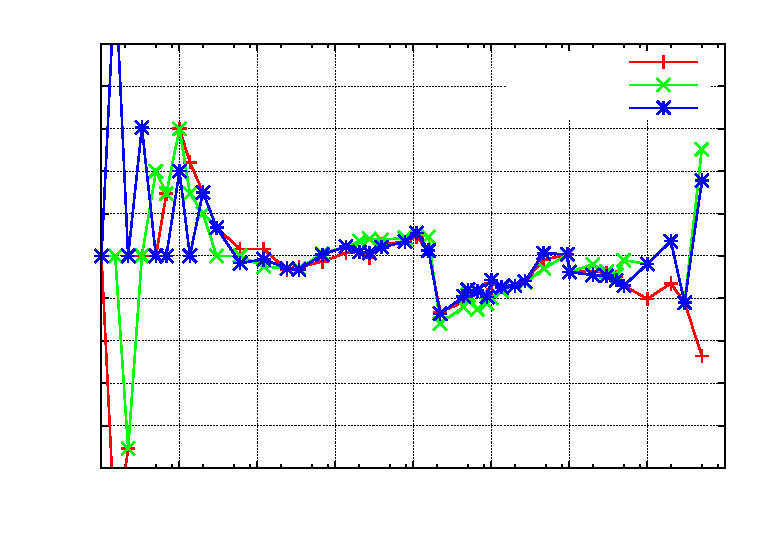
\includegraphics{../GNU/Mega8Lres}}%
    \gplfronttext
  \end{picture}%
\endgroup
}
    \caption{mit drei ATmega8L}
    \label{fig:mega8Lres}
  \end{subfigure}
\caption{Relativer Fehler für Widerstands-Messungen}
\end{figure}

\begin{figure}[H]
\centering
% GNUPLOT: LaTeX picture with Postscript
\begingroup
  \makeatletter
  \providecommand\color[2][]{%
    \GenericError{(gnuplot) \space\space\space\@spaces}{%
      Package color not loaded in conjunction with
      terminal option `colourtext'%
    }{See the gnuplot documentation for explanation.%
    }{Either use 'blacktext' in gnuplot or load the package
      color.sty in LaTeX.}%
    \renewcommand\color[2][]{}%
  }%
  \providecommand\includegraphics[2][]{%
    \GenericError{(gnuplot) \space\space\space\@spaces}{%
      Package graphicx or graphics not loaded%
    }{See the gnuplot documentation for explanation.%
    }{The gnuplot epslatex terminal needs graphicx.sty or graphics.sty.}%
    \renewcommand\includegraphics[2][]{}%
  }%
  \providecommand\rotatebox[2]{#2}%
  \@ifundefined{ifGPcolor}{%
    \newif\ifGPcolor
    \GPcolortrue
  }{}%
  \@ifundefined{ifGPblacktext}{%
    \newif\ifGPblacktext
    \GPblacktexttrue
  }{}%
  % define a \g@addto@macro without @ in the name:
  \let\gplgaddtomacro\g@addto@macro
  % define empty templates for all commands taking text:
  \gdef\gplbacktext{}%
  \gdef\gplfronttext{}%
  \makeatother
  \ifGPblacktext
    % no textcolor at all
    \def\colorrgb#1{}%
    \def\colorgray#1{}%
  \else
    % gray or color?
    \ifGPcolor
      \def\colorrgb#1{\color[rgb]{#1}}%
      \def\colorgray#1{\color[gray]{#1}}%
      \expandafter\def\csname LTw\endcsname{\color{white}}%
      \expandafter\def\csname LTb\endcsname{\color{black}}%
      \expandafter\def\csname LTa\endcsname{\color{black}}%
      \expandafter\def\csname LT0\endcsname{\color[rgb]{1,0,0}}%
      \expandafter\def\csname LT1\endcsname{\color[rgb]{0,1,0}}%
      \expandafter\def\csname LT2\endcsname{\color[rgb]{0,0,1}}%
      \expandafter\def\csname LT3\endcsname{\color[rgb]{1,0,1}}%
      \expandafter\def\csname LT4\endcsname{\color[rgb]{0,1,1}}%
      \expandafter\def\csname LT5\endcsname{\color[rgb]{1,1,0}}%
      \expandafter\def\csname LT6\endcsname{\color[rgb]{0,0,0}}%
      \expandafter\def\csname LT7\endcsname{\color[rgb]{1,0.3,0}}%
      \expandafter\def\csname LT8\endcsname{\color[rgb]{0.5,0.5,0.5}}%
    \else
      % gray
      \def\colorrgb#1{\color{black}}%
      \def\colorgray#1{\color[gray]{#1}}%
      \expandafter\def\csname LTw\endcsname{\color{white}}%
      \expandafter\def\csname LTb\endcsname{\color{black}}%
      \expandafter\def\csname LTa\endcsname{\color{black}}%
      \expandafter\def\csname LT0\endcsname{\color{black}}%
      \expandafter\def\csname LT1\endcsname{\color{black}}%
      \expandafter\def\csname LT2\endcsname{\color{black}}%
      \expandafter\def\csname LT3\endcsname{\color{black}}%
      \expandafter\def\csname LT4\endcsname{\color{black}}%
      \expandafter\def\csname LT5\endcsname{\color{black}}%
      \expandafter\def\csname LT6\endcsname{\color{black}}%
      \expandafter\def\csname LT7\endcsname{\color{black}}%
      \expandafter\def\csname LT8\endcsname{\color{black}}%
    \fi
  \fi
  \setlength{\unitlength}{0.0500bp}%
  \begin{picture}(7200.00,5040.00)%
    \gplgaddtomacro\gplbacktext{%
      \csname LTb\endcsname%
      \put(682,704){\makebox(0,0)[r]{\strut{}-5}}%
      \csname LTb\endcsname%
      \put(682,1111){\makebox(0,0)[r]{\strut{}-4}}%
      \csname LTb\endcsname%
      \put(682,1518){\makebox(0,0)[r]{\strut{}-3}}%
      \csname LTb\endcsname%
      \put(682,1925){\makebox(0,0)[r]{\strut{}-2}}%
      \csname LTb\endcsname%
      \put(682,2332){\makebox(0,0)[r]{\strut{}-1}}%
      \csname LTb\endcsname%
      \put(682,2740){\makebox(0,0)[r]{\strut{} 0}}%
      \csname LTb\endcsname%
      \put(682,3147){\makebox(0,0)[r]{\strut{} 1}}%
      \csname LTb\endcsname%
      \put(682,3554){\makebox(0,0)[r]{\strut{} 2}}%
      \csname LTb\endcsname%
      \put(682,3961){\makebox(0,0)[r]{\strut{} 3}}%
      \csname LTb\endcsname%
      \put(682,4368){\makebox(0,0)[r]{\strut{} 4}}%
      \csname LTb\endcsname%
      \put(682,4775){\makebox(0,0)[r]{\strut{} 5}}%
      \csname LTb\endcsname%
      \put(814,484){\makebox(0,0){\strut{}1 }}%
      \csname LTb\endcsname%
      \put(1563,484){\makebox(0,0){\strut{}10 }}%
      \csname LTb\endcsname%
      \put(2311,484){\makebox(0,0){\strut{}100 }}%
      \csname LTb\endcsname%
      \put(3060,484){\makebox(0,0){\strut{}1k}}%
      \csname LTb\endcsname%
      \put(3809,484){\makebox(0,0){\strut{}10k}}%
      \csname LTb\endcsname%
      \put(4557,484){\makebox(0,0){\strut{}100k}}%
      \csname LTb\endcsname%
      \put(5306,484){\makebox(0,0){\strut{}1M}}%
      \csname LTb\endcsname%
      \put(6054,484){\makebox(0,0){\strut{}10M}}%
      \csname LTb\endcsname%
      \put(6803,484){\makebox(0,0){\strut{}100M}}%
      \put(176,2739){\rotatebox{-270}{\makebox(0,0){\strut{}Error / Percent}}}%
      \put(3808,154){\makebox(0,0){\strut{}Resistor value / Ohm}}%
    }%
    \gplgaddtomacro\gplfronttext{%
      \csname LTb\endcsname%
      \put(5753,4602){\makebox(0,0)[r]{\strut{}Mega168}}%
      \csname LTb\endcsname%
      \put(5753,4382){\makebox(0,0)[r]{\strut{}Mega168as}}%
    }%
    \gplbacktext
    \put(0,0){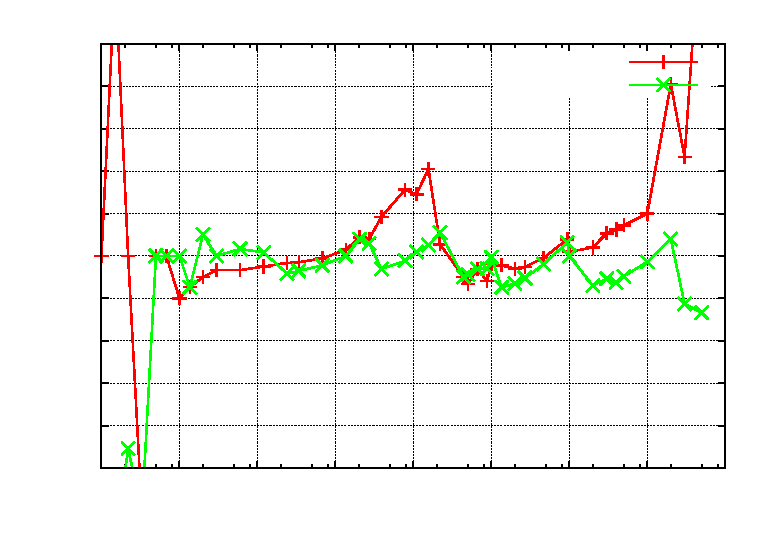
\includegraphics{../GNU/Mega168res}}%
    \gplfronttext
  \end{picture}%
\endgroup

\caption{Relativer Fehler für Widerstand-Messungen mit ATmega168 }
\label{fig:mega168res}
\end{figure}

Das Diagramm \ref{fig:m168res_all} zeigt die Messfehler von drei ATmega168-Prozessoren vor der Kalibration als Punkte, nach der
Kalibration als Linie. Entsprechend werden die Messfehler von drei ATmega168A in Abbildung \ref{fig:m168ares_all} und
die Messfehler von drei ATmega328P in Abbildung \ref{fig:m168pres_all} gezeigt.
Die Messfehler der ATmega328 werden in den Abbildungen \ref{fig:m328res_all} und \ref{fig:m328pres_all} gezeigt.
Nach der automatischen Kalibration bleibt der Messfehler mit einer Ausnahme (ATmega328P-13, \(22 k\Omega\)) im Widerstandsbereich
\(10~\Omega~-~20 M\Omega\) im Bereich \(\pm1~\%\).
Vor der Kalibration können die Messfehler bei einigen Prozessoren bis \(\pm~3\%\) betragen.
Der Fehler wird verursacht durch die AUTOSCALE\_ADC-Umschaltung der ADC-Referenz.
Durch den direkten Vergleich einer Kondensatorspannung von unter 1~V, einmal mit der VCC-Referenz und nochmal mit
der internen ADC-Referenz gemessen, kann der Fehler ausgeglichen werden.
In diesem Fall wird die Spannung mit dem gleichen Multiplexer-Kanal gemessen und die Bandgap-Referenz ist auf den AREF-Pin
aufgeschaltet.
Die direkte Vermessung der Bandgap-Referenz durch die direkte Wahl des Multiplexer-Eingangs führt leider zu diesem Offset,
der entweder manuell mit der Option REF\_R\_KORR oder automatisch mit der Option AUTO\_CAL des Selbsttestes beseitigt werden kann.
Im AUTO\_CAL-Modus ist REF\_R\_KORR ein zusätzlicher Offset zur automatisch gefundenen Spannungsdifferenz.

\begin{figure}[H]
  \begin{subfigure}[b]{9cm}
    \centering
    \resizebox{9cm}{!}{% GNUPLOT: LaTeX picture with Postscript
\begingroup
  \makeatletter
  \providecommand\color[2][]{%
    \GenericError{(gnuplot) \space\space\space\@spaces}{%
      Package color not loaded in conjunction with
      terminal option `colourtext'%
    }{See the gnuplot documentation for explanation.%
    }{Either use 'blacktext' in gnuplot or load the package
      color.sty in LaTeX.}%
    \renewcommand\color[2][]{}%
  }%
  \providecommand\includegraphics[2][]{%
    \GenericError{(gnuplot) \space\space\space\@spaces}{%
      Package graphicx or graphics not loaded%
    }{See the gnuplot documentation for explanation.%
    }{The gnuplot epslatex terminal needs graphicx.sty or graphics.sty.}%
    \renewcommand\includegraphics[2][]{}%
  }%
  \providecommand\rotatebox[2]{#2}%
  \@ifundefined{ifGPcolor}{%
    \newif\ifGPcolor
    \GPcolortrue
  }{}%
  \@ifundefined{ifGPblacktext}{%
    \newif\ifGPblacktext
    \GPblacktexttrue
  }{}%
  % define a \g@addto@macro without @ in the name:
  \let\gplgaddtomacro\g@addto@macro
  % define empty templates for all commands taking text:
  \gdef\gplbacktext{}%
  \gdef\gplfronttext{}%
  \makeatother
  \ifGPblacktext
    % no textcolor at all
    \def\colorrgb#1{}%
    \def\colorgray#1{}%
  \else
    % gray or color?
    \ifGPcolor
      \def\colorrgb#1{\color[rgb]{#1}}%
      \def\colorgray#1{\color[gray]{#1}}%
      \expandafter\def\csname LTw\endcsname{\color{white}}%
      \expandafter\def\csname LTb\endcsname{\color{black}}%
      \expandafter\def\csname LTa\endcsname{\color{black}}%
      \expandafter\def\csname LT0\endcsname{\color[rgb]{1,0,0}}%
      \expandafter\def\csname LT1\endcsname{\color[rgb]{0,1,0}}%
      \expandafter\def\csname LT2\endcsname{\color[rgb]{0,0,1}}%
      \expandafter\def\csname LT3\endcsname{\color[rgb]{1,0,1}}%
      \expandafter\def\csname LT4\endcsname{\color[rgb]{0,1,1}}%
      \expandafter\def\csname LT5\endcsname{\color[rgb]{1,1,0}}%
      \expandafter\def\csname LT6\endcsname{\color[rgb]{0,0,0}}%
      \expandafter\def\csname LT7\endcsname{\color[rgb]{1,0.3,0}}%
      \expandafter\def\csname LT8\endcsname{\color[rgb]{0.5,0.5,0.5}}%
    \else
      % gray
      \def\colorrgb#1{\color{black}}%
      \def\colorgray#1{\color[gray]{#1}}%
      \expandafter\def\csname LTw\endcsname{\color{white}}%
      \expandafter\def\csname LTb\endcsname{\color{black}}%
      \expandafter\def\csname LTa\endcsname{\color{black}}%
      \expandafter\def\csname LT0\endcsname{\color{black}}%
      \expandafter\def\csname LT1\endcsname{\color{black}}%
      \expandafter\def\csname LT2\endcsname{\color{black}}%
      \expandafter\def\csname LT3\endcsname{\color{black}}%
      \expandafter\def\csname LT4\endcsname{\color{black}}%
      \expandafter\def\csname LT5\endcsname{\color{black}}%
      \expandafter\def\csname LT6\endcsname{\color{black}}%
      \expandafter\def\csname LT7\endcsname{\color{black}}%
      \expandafter\def\csname LT8\endcsname{\color{black}}%
    \fi
  \fi
  \setlength{\unitlength}{0.0500bp}%
  \begin{picture}(7200.00,5040.00)%
    \gplgaddtomacro\gplbacktext{%
      \csname LTb\endcsname%
      \put(682,704){\makebox(0,0)[r]{\strut{}-5}}%
      \csname LTb\endcsname%
      \put(682,1111){\makebox(0,0)[r]{\strut{}-4}}%
      \csname LTb\endcsname%
      \put(682,1518){\makebox(0,0)[r]{\strut{}-3}}%
      \csname LTb\endcsname%
      \put(682,1925){\makebox(0,0)[r]{\strut{}-2}}%
      \csname LTb\endcsname%
      \put(682,2332){\makebox(0,0)[r]{\strut{}-1}}%
      \csname LTb\endcsname%
      \put(682,2740){\makebox(0,0)[r]{\strut{} 0}}%
      \csname LTb\endcsname%
      \put(682,3147){\makebox(0,0)[r]{\strut{} 1}}%
      \csname LTb\endcsname%
      \put(682,3554){\makebox(0,0)[r]{\strut{} 2}}%
      \csname LTb\endcsname%
      \put(682,3961){\makebox(0,0)[r]{\strut{} 3}}%
      \csname LTb\endcsname%
      \put(682,4368){\makebox(0,0)[r]{\strut{} 4}}%
      \csname LTb\endcsname%
      \put(682,4775){\makebox(0,0)[r]{\strut{} 5}}%
      \csname LTb\endcsname%
      \put(814,484){\makebox(0,0){\strut{}1 }}%
      \csname LTb\endcsname%
      \put(1563,484){\makebox(0,0){\strut{}10 }}%
      \csname LTb\endcsname%
      \put(2311,484){\makebox(0,0){\strut{}100 }}%
      \csname LTb\endcsname%
      \put(3060,484){\makebox(0,0){\strut{}1k}}%
      \csname LTb\endcsname%
      \put(3809,484){\makebox(0,0){\strut{}10k}}%
      \csname LTb\endcsname%
      \put(4557,484){\makebox(0,0){\strut{}100k}}%
      \csname LTb\endcsname%
      \put(5306,484){\makebox(0,0){\strut{}1M}}%
      \csname LTb\endcsname%
      \put(6054,484){\makebox(0,0){\strut{}10M}}%
      \csname LTb\endcsname%
      \put(6803,484){\makebox(0,0){\strut{}100M}}%
      \put(176,2739){\rotatebox{-270}{\makebox(0,0){\strut{}Error / Percent}}}%
      \put(3808,154){\makebox(0,0){\strut{}Resistor value / Ohm}}%
    }%
    \gplgaddtomacro\gplfronttext{%
      \csname LTb\endcsname%
      \put(5753,4602){\makebox(0,0)[r]{\strut{}m168-1}}%
      \csname LTb\endcsname%
      \put(5753,4382){\makebox(0,0)[r]{\strut{}m168-2}}%
      \csname LTb\endcsname%
      \put(5753,4162){\makebox(0,0)[r]{\strut{}m168-3}}%
      \csname LTb\endcsname%
      \put(5753,3942){\makebox(0,0)[r]{\strut{}m168-1}}%
      \csname LTb\endcsname%
      \put(5753,3722){\makebox(0,0)[r]{\strut{}m168-2}}%
      \csname LTb\endcsname%
      \put(5753,3502){\makebox(0,0)[r]{\strut{}m168-3}}%
    }%
    \gplbacktext
    \put(0,0){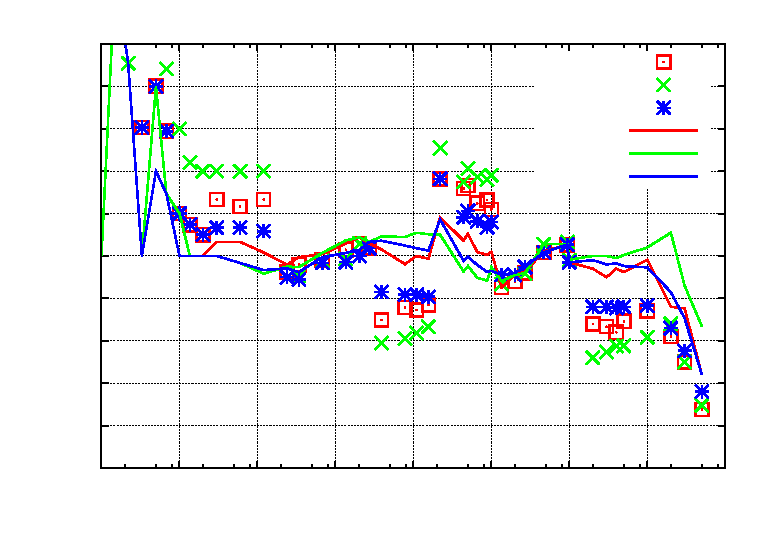
\includegraphics{../GNU/m168res_all}}%
    \gplfronttext
  \end{picture}%
\endgroup
}
    \caption{mit drei ATmega168}
    \label{fig:m168res_all}
  \end{subfigure}
  ~
  \begin{subfigure}[b]{9cm}
    \centering
    \resizebox{9cm}{!}{% GNUPLOT: LaTeX picture with Postscript
\begingroup
  \makeatletter
  \providecommand\color[2][]{%
    \GenericError{(gnuplot) \space\space\space\@spaces}{%
      Package color not loaded in conjunction with
      terminal option `colourtext'%
    }{See the gnuplot documentation for explanation.%
    }{Either use 'blacktext' in gnuplot or load the package
      color.sty in LaTeX.}%
    \renewcommand\color[2][]{}%
  }%
  \providecommand\includegraphics[2][]{%
    \GenericError{(gnuplot) \space\space\space\@spaces}{%
      Package graphicx or graphics not loaded%
    }{See the gnuplot documentation for explanation.%
    }{The gnuplot epslatex terminal needs graphicx.sty or graphics.sty.}%
    \renewcommand\includegraphics[2][]{}%
  }%
  \providecommand\rotatebox[2]{#2}%
  \@ifundefined{ifGPcolor}{%
    \newif\ifGPcolor
    \GPcolortrue
  }{}%
  \@ifundefined{ifGPblacktext}{%
    \newif\ifGPblacktext
    \GPblacktexttrue
  }{}%
  % define a \g@addto@macro without @ in the name:
  \let\gplgaddtomacro\g@addto@macro
  % define empty templates for all commands taking text:
  \gdef\gplbacktext{}%
  \gdef\gplfronttext{}%
  \makeatother
  \ifGPblacktext
    % no textcolor at all
    \def\colorrgb#1{}%
    \def\colorgray#1{}%
  \else
    % gray or color?
    \ifGPcolor
      \def\colorrgb#1{\color[rgb]{#1}}%
      \def\colorgray#1{\color[gray]{#1}}%
      \expandafter\def\csname LTw\endcsname{\color{white}}%
      \expandafter\def\csname LTb\endcsname{\color{black}}%
      \expandafter\def\csname LTa\endcsname{\color{black}}%
      \expandafter\def\csname LT0\endcsname{\color[rgb]{1,0,0}}%
      \expandafter\def\csname LT1\endcsname{\color[rgb]{0,1,0}}%
      \expandafter\def\csname LT2\endcsname{\color[rgb]{0,0,1}}%
      \expandafter\def\csname LT3\endcsname{\color[rgb]{1,0,1}}%
      \expandafter\def\csname LT4\endcsname{\color[rgb]{0,1,1}}%
      \expandafter\def\csname LT5\endcsname{\color[rgb]{1,1,0}}%
      \expandafter\def\csname LT6\endcsname{\color[rgb]{0,0,0}}%
      \expandafter\def\csname LT7\endcsname{\color[rgb]{1,0.3,0}}%
      \expandafter\def\csname LT8\endcsname{\color[rgb]{0.5,0.5,0.5}}%
    \else
      % gray
      \def\colorrgb#1{\color{black}}%
      \def\colorgray#1{\color[gray]{#1}}%
      \expandafter\def\csname LTw\endcsname{\color{white}}%
      \expandafter\def\csname LTb\endcsname{\color{black}}%
      \expandafter\def\csname LTa\endcsname{\color{black}}%
      \expandafter\def\csname LT0\endcsname{\color{black}}%
      \expandafter\def\csname LT1\endcsname{\color{black}}%
      \expandafter\def\csname LT2\endcsname{\color{black}}%
      \expandafter\def\csname LT3\endcsname{\color{black}}%
      \expandafter\def\csname LT4\endcsname{\color{black}}%
      \expandafter\def\csname LT5\endcsname{\color{black}}%
      \expandafter\def\csname LT6\endcsname{\color{black}}%
      \expandafter\def\csname LT7\endcsname{\color{black}}%
      \expandafter\def\csname LT8\endcsname{\color{black}}%
    \fi
  \fi
  \setlength{\unitlength}{0.0500bp}%
  \begin{picture}(7200.00,5040.00)%
    \gplgaddtomacro\gplbacktext{%
      \csname LTb\endcsname%
      \put(682,704){\makebox(0,0)[r]{\strut{}-5}}%
      \csname LTb\endcsname%
      \put(682,1111){\makebox(0,0)[r]{\strut{}-4}}%
      \csname LTb\endcsname%
      \put(682,1518){\makebox(0,0)[r]{\strut{}-3}}%
      \csname LTb\endcsname%
      \put(682,1925){\makebox(0,0)[r]{\strut{}-2}}%
      \csname LTb\endcsname%
      \put(682,2332){\makebox(0,0)[r]{\strut{}-1}}%
      \csname LTb\endcsname%
      \put(682,2740){\makebox(0,0)[r]{\strut{} 0}}%
      \csname LTb\endcsname%
      \put(682,3147){\makebox(0,0)[r]{\strut{} 1}}%
      \csname LTb\endcsname%
      \put(682,3554){\makebox(0,0)[r]{\strut{} 2}}%
      \csname LTb\endcsname%
      \put(682,3961){\makebox(0,0)[r]{\strut{} 3}}%
      \csname LTb\endcsname%
      \put(682,4368){\makebox(0,0)[r]{\strut{} 4}}%
      \csname LTb\endcsname%
      \put(682,4775){\makebox(0,0)[r]{\strut{} 5}}%
      \csname LTb\endcsname%
      \put(814,484){\makebox(0,0){\strut{}1 }}%
      \csname LTb\endcsname%
      \put(1563,484){\makebox(0,0){\strut{}10 }}%
      \csname LTb\endcsname%
      \put(2311,484){\makebox(0,0){\strut{}100 }}%
      \csname LTb\endcsname%
      \put(3060,484){\makebox(0,0){\strut{}1k}}%
      \csname LTb\endcsname%
      \put(3809,484){\makebox(0,0){\strut{}10k}}%
      \csname LTb\endcsname%
      \put(4557,484){\makebox(0,0){\strut{}100k}}%
      \csname LTb\endcsname%
      \put(5306,484){\makebox(0,0){\strut{}1M}}%
      \csname LTb\endcsname%
      \put(6054,484){\makebox(0,0){\strut{}10M}}%
      \csname LTb\endcsname%
      \put(6803,484){\makebox(0,0){\strut{}100M}}%
      \put(176,2739){\rotatebox{-270}{\makebox(0,0){\strut{}Error / Percent}}}%
      \put(3808,154){\makebox(0,0){\strut{}Resistor value / Ohm}}%
    }%
    \gplgaddtomacro\gplfronttext{%
      \csname LTb\endcsname%
      \put(5753,4602){\makebox(0,0)[r]{\strut{}m168a-4}}%
      \csname LTb\endcsname%
      \put(5753,4382){\makebox(0,0)[r]{\strut{}m168a-5}}%
      \csname LTb\endcsname%
      \put(5753,4162){\makebox(0,0)[r]{\strut{}m168a-6}}%
      \csname LTb\endcsname%
      \put(5753,3942){\makebox(0,0)[r]{\strut{}m168a-4}}%
      \csname LTb\endcsname%
      \put(5753,3722){\makebox(0,0)[r]{\strut{}m168a-5}}%
      \csname LTb\endcsname%
      \put(5753,3502){\makebox(0,0)[r]{\strut{}m168a-6}}%
    }%
    \gplbacktext
    \put(0,0){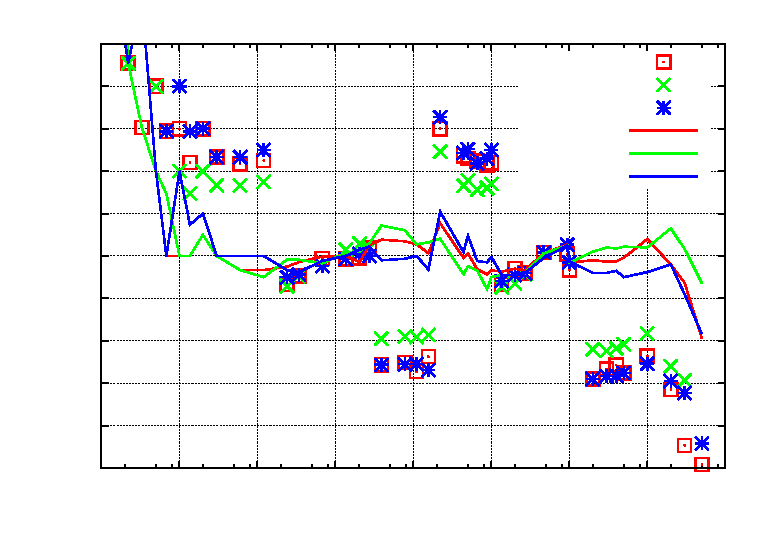
\includegraphics{../GNU/m168ares_all}}%
    \gplfronttext
  \end{picture}%
\endgroup
}
    \caption{mit drei ATmega168A}
    \label{fig:m168ares_all}
  \end{subfigure}
\caption{Relativer Fehler für Widerstands-Messungen}
\end{figure}

\begin{figure}[H]
\centering
% GNUPLOT: LaTeX picture with Postscript
\begingroup
  \makeatletter
  \providecommand\color[2][]{%
    \GenericError{(gnuplot) \space\space\space\@spaces}{%
      Package color not loaded in conjunction with
      terminal option `colourtext'%
    }{See the gnuplot documentation for explanation.%
    }{Either use 'blacktext' in gnuplot or load the package
      color.sty in LaTeX.}%
    \renewcommand\color[2][]{}%
  }%
  \providecommand\includegraphics[2][]{%
    \GenericError{(gnuplot) \space\space\space\@spaces}{%
      Package graphicx or graphics not loaded%
    }{See the gnuplot documentation for explanation.%
    }{The gnuplot epslatex terminal needs graphicx.sty or graphics.sty.}%
    \renewcommand\includegraphics[2][]{}%
  }%
  \providecommand\rotatebox[2]{#2}%
  \@ifundefined{ifGPcolor}{%
    \newif\ifGPcolor
    \GPcolortrue
  }{}%
  \@ifundefined{ifGPblacktext}{%
    \newif\ifGPblacktext
    \GPblacktexttrue
  }{}%
  % define a \g@addto@macro without @ in the name:
  \let\gplgaddtomacro\g@addto@macro
  % define empty templates for all commands taking text:
  \gdef\gplbacktext{}%
  \gdef\gplfronttext{}%
  \makeatother
  \ifGPblacktext
    % no textcolor at all
    \def\colorrgb#1{}%
    \def\colorgray#1{}%
  \else
    % gray or color?
    \ifGPcolor
      \def\colorrgb#1{\color[rgb]{#1}}%
      \def\colorgray#1{\color[gray]{#1}}%
      \expandafter\def\csname LTw\endcsname{\color{white}}%
      \expandafter\def\csname LTb\endcsname{\color{black}}%
      \expandafter\def\csname LTa\endcsname{\color{black}}%
      \expandafter\def\csname LT0\endcsname{\color[rgb]{1,0,0}}%
      \expandafter\def\csname LT1\endcsname{\color[rgb]{0,1,0}}%
      \expandafter\def\csname LT2\endcsname{\color[rgb]{0,0,1}}%
      \expandafter\def\csname LT3\endcsname{\color[rgb]{1,0,1}}%
      \expandafter\def\csname LT4\endcsname{\color[rgb]{0,1,1}}%
      \expandafter\def\csname LT5\endcsname{\color[rgb]{1,1,0}}%
      \expandafter\def\csname LT6\endcsname{\color[rgb]{0,0,0}}%
      \expandafter\def\csname LT7\endcsname{\color[rgb]{1,0.3,0}}%
      \expandafter\def\csname LT8\endcsname{\color[rgb]{0.5,0.5,0.5}}%
    \else
      % gray
      \def\colorrgb#1{\color{black}}%
      \def\colorgray#1{\color[gray]{#1}}%
      \expandafter\def\csname LTw\endcsname{\color{white}}%
      \expandafter\def\csname LTb\endcsname{\color{black}}%
      \expandafter\def\csname LTa\endcsname{\color{black}}%
      \expandafter\def\csname LT0\endcsname{\color{black}}%
      \expandafter\def\csname LT1\endcsname{\color{black}}%
      \expandafter\def\csname LT2\endcsname{\color{black}}%
      \expandafter\def\csname LT3\endcsname{\color{black}}%
      \expandafter\def\csname LT4\endcsname{\color{black}}%
      \expandafter\def\csname LT5\endcsname{\color{black}}%
      \expandafter\def\csname LT6\endcsname{\color{black}}%
      \expandafter\def\csname LT7\endcsname{\color{black}}%
      \expandafter\def\csname LT8\endcsname{\color{black}}%
    \fi
  \fi
  \setlength{\unitlength}{0.0500bp}%
  \begin{picture}(7200.00,5040.00)%
    \gplgaddtomacro\gplbacktext{%
      \csname LTb\endcsname%
      \put(682,704){\makebox(0,0)[r]{\strut{}-5}}%
      \csname LTb\endcsname%
      \put(682,1111){\makebox(0,0)[r]{\strut{}-4}}%
      \csname LTb\endcsname%
      \put(682,1518){\makebox(0,0)[r]{\strut{}-3}}%
      \csname LTb\endcsname%
      \put(682,1925){\makebox(0,0)[r]{\strut{}-2}}%
      \csname LTb\endcsname%
      \put(682,2332){\makebox(0,0)[r]{\strut{}-1}}%
      \csname LTb\endcsname%
      \put(682,2740){\makebox(0,0)[r]{\strut{} 0}}%
      \csname LTb\endcsname%
      \put(682,3147){\makebox(0,0)[r]{\strut{} 1}}%
      \csname LTb\endcsname%
      \put(682,3554){\makebox(0,0)[r]{\strut{} 2}}%
      \csname LTb\endcsname%
      \put(682,3961){\makebox(0,0)[r]{\strut{} 3}}%
      \csname LTb\endcsname%
      \put(682,4368){\makebox(0,0)[r]{\strut{} 4}}%
      \csname LTb\endcsname%
      \put(682,4775){\makebox(0,0)[r]{\strut{} 5}}%
      \csname LTb\endcsname%
      \put(814,484){\makebox(0,0){\strut{}1 }}%
      \csname LTb\endcsname%
      \put(1563,484){\makebox(0,0){\strut{}10 }}%
      \csname LTb\endcsname%
      \put(2311,484){\makebox(0,0){\strut{}100 }}%
      \csname LTb\endcsname%
      \put(3060,484){\makebox(0,0){\strut{}1k}}%
      \csname LTb\endcsname%
      \put(3809,484){\makebox(0,0){\strut{}10k}}%
      \csname LTb\endcsname%
      \put(4557,484){\makebox(0,0){\strut{}100k}}%
      \csname LTb\endcsname%
      \put(5306,484){\makebox(0,0){\strut{}1M}}%
      \csname LTb\endcsname%
      \put(6054,484){\makebox(0,0){\strut{}10M}}%
      \csname LTb\endcsname%
      \put(6803,484){\makebox(0,0){\strut{}100M}}%
      \put(176,2739){\rotatebox{-270}{\makebox(0,0){\strut{}Error / Percent}}}%
      \put(3808,154){\makebox(0,0){\strut{}Resistor value / Ohm}}%
    }%
    \gplgaddtomacro\gplfronttext{%
      \csname LTb\endcsname%
      \put(5753,4602){\makebox(0,0)[r]{\strut{}m168p-7}}%
      \csname LTb\endcsname%
      \put(5753,4382){\makebox(0,0)[r]{\strut{}m168p-8}}%
      \csname LTb\endcsname%
      \put(5753,4162){\makebox(0,0)[r]{\strut{}m168p-9}}%
      \csname LTb\endcsname%
      \put(5753,3942){\makebox(0,0)[r]{\strut{}m168p-7}}%
      \csname LTb\endcsname%
      \put(5753,3722){\makebox(0,0)[r]{\strut{}m168p-8}}%
      \csname LTb\endcsname%
      \put(5753,3502){\makebox(0,0)[r]{\strut{}m168p-9}}%
    }%
    \gplbacktext
    \put(0,0){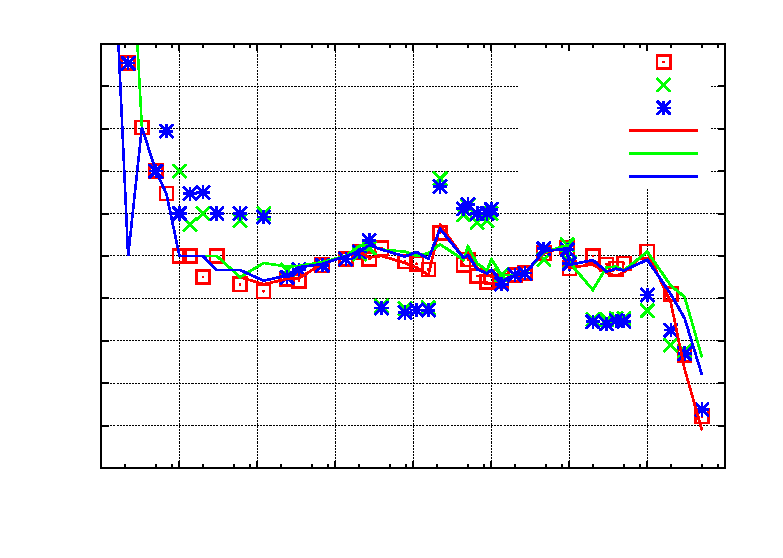
\includegraphics{../GNU/m168pres_all}}%
    \gplfronttext
  \end{picture}%
\endgroup

\caption{Relativer Fehler für Widerstands-Messungen mit drei ATmega168P }
\label{fig:m168pres_all}
\end{figure}

\begin{figure}[H]
  \begin{subfigure}[b]{9cm}
    \centering
    \resizebox{9cm}{!}{% GNUPLOT: LaTeX picture with Postscript
\begingroup
  \makeatletter
  \providecommand\color[2][]{%
    \GenericError{(gnuplot) \space\space\space\@spaces}{%
      Package color not loaded in conjunction with
      terminal option `colourtext'%
    }{See the gnuplot documentation for explanation.%
    }{Either use 'blacktext' in gnuplot or load the package
      color.sty in LaTeX.}%
    \renewcommand\color[2][]{}%
  }%
  \providecommand\includegraphics[2][]{%
    \GenericError{(gnuplot) \space\space\space\@spaces}{%
      Package graphicx or graphics not loaded%
    }{See the gnuplot documentation for explanation.%
    }{The gnuplot epslatex terminal needs graphicx.sty or graphics.sty.}%
    \renewcommand\includegraphics[2][]{}%
  }%
  \providecommand\rotatebox[2]{#2}%
  \@ifundefined{ifGPcolor}{%
    \newif\ifGPcolor
    \GPcolortrue
  }{}%
  \@ifundefined{ifGPblacktext}{%
    \newif\ifGPblacktext
    \GPblacktexttrue
  }{}%
  % define a \g@addto@macro without @ in the name:
  \let\gplgaddtomacro\g@addto@macro
  % define empty templates for all commands taking text:
  \gdef\gplbacktext{}%
  \gdef\gplfronttext{}%
  \makeatother
  \ifGPblacktext
    % no textcolor at all
    \def\colorrgb#1{}%
    \def\colorgray#1{}%
  \else
    % gray or color?
    \ifGPcolor
      \def\colorrgb#1{\color[rgb]{#1}}%
      \def\colorgray#1{\color[gray]{#1}}%
      \expandafter\def\csname LTw\endcsname{\color{white}}%
      \expandafter\def\csname LTb\endcsname{\color{black}}%
      \expandafter\def\csname LTa\endcsname{\color{black}}%
      \expandafter\def\csname LT0\endcsname{\color[rgb]{1,0,0}}%
      \expandafter\def\csname LT1\endcsname{\color[rgb]{0,1,0}}%
      \expandafter\def\csname LT2\endcsname{\color[rgb]{0,0,1}}%
      \expandafter\def\csname LT3\endcsname{\color[rgb]{1,0,1}}%
      \expandafter\def\csname LT4\endcsname{\color[rgb]{0,1,1}}%
      \expandafter\def\csname LT5\endcsname{\color[rgb]{1,1,0}}%
      \expandafter\def\csname LT6\endcsname{\color[rgb]{0,0,0}}%
      \expandafter\def\csname LT7\endcsname{\color[rgb]{1,0.3,0}}%
      \expandafter\def\csname LT8\endcsname{\color[rgb]{0.5,0.5,0.5}}%
    \else
      % gray
      \def\colorrgb#1{\color{black}}%
      \def\colorgray#1{\color[gray]{#1}}%
      \expandafter\def\csname LTw\endcsname{\color{white}}%
      \expandafter\def\csname LTb\endcsname{\color{black}}%
      \expandafter\def\csname LTa\endcsname{\color{black}}%
      \expandafter\def\csname LT0\endcsname{\color{black}}%
      \expandafter\def\csname LT1\endcsname{\color{black}}%
      \expandafter\def\csname LT2\endcsname{\color{black}}%
      \expandafter\def\csname LT3\endcsname{\color{black}}%
      \expandafter\def\csname LT4\endcsname{\color{black}}%
      \expandafter\def\csname LT5\endcsname{\color{black}}%
      \expandafter\def\csname LT6\endcsname{\color{black}}%
      \expandafter\def\csname LT7\endcsname{\color{black}}%
      \expandafter\def\csname LT8\endcsname{\color{black}}%
    \fi
  \fi
  \setlength{\unitlength}{0.0500bp}%
  \begin{picture}(7200.00,5040.00)%
    \gplgaddtomacro\gplbacktext{%
      \csname LTb\endcsname%
      \put(682,704){\makebox(0,0)[r]{\strut{}-5}}%
      \csname LTb\endcsname%
      \put(682,1111){\makebox(0,0)[r]{\strut{}-4}}%
      \csname LTb\endcsname%
      \put(682,1518){\makebox(0,0)[r]{\strut{}-3}}%
      \csname LTb\endcsname%
      \put(682,1925){\makebox(0,0)[r]{\strut{}-2}}%
      \csname LTb\endcsname%
      \put(682,2332){\makebox(0,0)[r]{\strut{}-1}}%
      \csname LTb\endcsname%
      \put(682,2740){\makebox(0,0)[r]{\strut{} 0}}%
      \csname LTb\endcsname%
      \put(682,3147){\makebox(0,0)[r]{\strut{} 1}}%
      \csname LTb\endcsname%
      \put(682,3554){\makebox(0,0)[r]{\strut{} 2}}%
      \csname LTb\endcsname%
      \put(682,3961){\makebox(0,0)[r]{\strut{} 3}}%
      \csname LTb\endcsname%
      \put(682,4368){\makebox(0,0)[r]{\strut{} 4}}%
      \csname LTb\endcsname%
      \put(682,4775){\makebox(0,0)[r]{\strut{} 5}}%
      \csname LTb\endcsname%
      \put(814,484){\makebox(0,0){\strut{}1 }}%
      \csname LTb\endcsname%
      \put(1563,484){\makebox(0,0){\strut{}10 }}%
      \csname LTb\endcsname%
      \put(2311,484){\makebox(0,0){\strut{}100 }}%
      \csname LTb\endcsname%
      \put(3060,484){\makebox(0,0){\strut{}1k}}%
      \csname LTb\endcsname%
      \put(3809,484){\makebox(0,0){\strut{}10k}}%
      \csname LTb\endcsname%
      \put(4557,484){\makebox(0,0){\strut{}100k}}%
      \csname LTb\endcsname%
      \put(5306,484){\makebox(0,0){\strut{}1M}}%
      \csname LTb\endcsname%
      \put(6054,484){\makebox(0,0){\strut{}10M}}%
      \csname LTb\endcsname%
      \put(6803,484){\makebox(0,0){\strut{}100M}}%
      \put(176,2739){\rotatebox{-270}{\makebox(0,0){\strut{}Error / Percent}}}%
      \put(3808,154){\makebox(0,0){\strut{}Resistor value / Ohm}}%
    }%
    \gplgaddtomacro\gplfronttext{%
      \csname LTb\endcsname%
      \put(5753,4602){\makebox(0,0)[r]{\strut{}m328-10}}%
      \csname LTb\endcsname%
      \put(5753,4382){\makebox(0,0)[r]{\strut{}m328-11}}%
      \csname LTb\endcsname%
      \put(5753,4162){\makebox(0,0)[r]{\strut{}m328-12}}%
      \csname LTb\endcsname%
      \put(5753,3942){\makebox(0,0)[r]{\strut{}m328-10}}%
      \csname LTb\endcsname%
      \put(5753,3722){\makebox(0,0)[r]{\strut{}m328-11}}%
      \csname LTb\endcsname%
      \put(5753,3502){\makebox(0,0)[r]{\strut{}m328-12}}%
    }%
    \gplbacktext
    \put(0,0){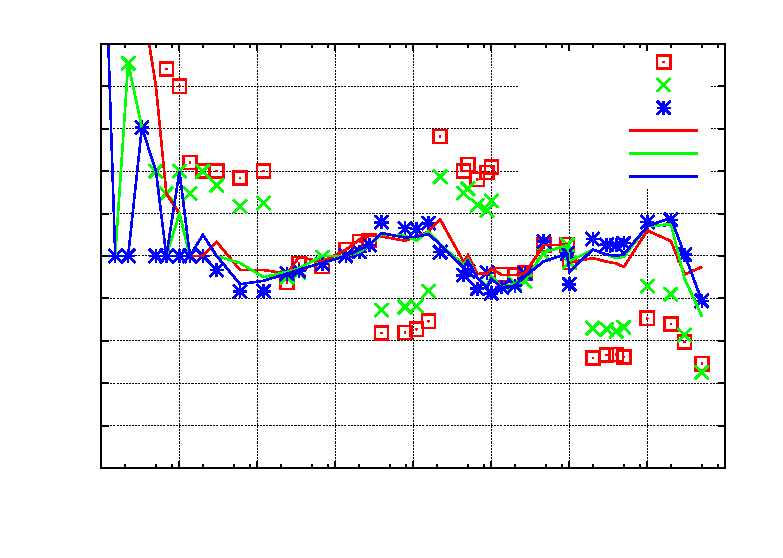
\includegraphics{../GNU/m328res_all}}%
    \gplfronttext
  \end{picture}%
\endgroup
}
    \caption{mit drei ATmega328}
    \label{fig:m328res_all}
  \end{subfigure}
  ~
  \begin{subfigure}[b]{9cm}
    \centering
    \resizebox{9cm}{!}{% GNUPLOT: LaTeX picture with Postscript
\begingroup
  \makeatletter
  \providecommand\color[2][]{%
    \GenericError{(gnuplot) \space\space\space\@spaces}{%
      Package color not loaded in conjunction with
      terminal option `colourtext'%
    }{See the gnuplot documentation for explanation.%
    }{Either use 'blacktext' in gnuplot or load the package
      color.sty in LaTeX.}%
    \renewcommand\color[2][]{}%
  }%
  \providecommand\includegraphics[2][]{%
    \GenericError{(gnuplot) \space\space\space\@spaces}{%
      Package graphicx or graphics not loaded%
    }{See the gnuplot documentation for explanation.%
    }{The gnuplot epslatex terminal needs graphicx.sty or graphics.sty.}%
    \renewcommand\includegraphics[2][]{}%
  }%
  \providecommand\rotatebox[2]{#2}%
  \@ifundefined{ifGPcolor}{%
    \newif\ifGPcolor
    \GPcolortrue
  }{}%
  \@ifundefined{ifGPblacktext}{%
    \newif\ifGPblacktext
    \GPblacktexttrue
  }{}%
  % define a \g@addto@macro without @ in the name:
  \let\gplgaddtomacro\g@addto@macro
  % define empty templates for all commands taking text:
  \gdef\gplbacktext{}%
  \gdef\gplfronttext{}%
  \makeatother
  \ifGPblacktext
    % no textcolor at all
    \def\colorrgb#1{}%
    \def\colorgray#1{}%
  \else
    % gray or color?
    \ifGPcolor
      \def\colorrgb#1{\color[rgb]{#1}}%
      \def\colorgray#1{\color[gray]{#1}}%
      \expandafter\def\csname LTw\endcsname{\color{white}}%
      \expandafter\def\csname LTb\endcsname{\color{black}}%
      \expandafter\def\csname LTa\endcsname{\color{black}}%
      \expandafter\def\csname LT0\endcsname{\color[rgb]{1,0,0}}%
      \expandafter\def\csname LT1\endcsname{\color[rgb]{0,1,0}}%
      \expandafter\def\csname LT2\endcsname{\color[rgb]{0,0,1}}%
      \expandafter\def\csname LT3\endcsname{\color[rgb]{1,0,1}}%
      \expandafter\def\csname LT4\endcsname{\color[rgb]{0,1,1}}%
      \expandafter\def\csname LT5\endcsname{\color[rgb]{1,1,0}}%
      \expandafter\def\csname LT6\endcsname{\color[rgb]{0,0,0}}%
      \expandafter\def\csname LT7\endcsname{\color[rgb]{1,0.3,0}}%
      \expandafter\def\csname LT8\endcsname{\color[rgb]{0.5,0.5,0.5}}%
    \else
      % gray
      \def\colorrgb#1{\color{black}}%
      \def\colorgray#1{\color[gray]{#1}}%
      \expandafter\def\csname LTw\endcsname{\color{white}}%
      \expandafter\def\csname LTb\endcsname{\color{black}}%
      \expandafter\def\csname LTa\endcsname{\color{black}}%
      \expandafter\def\csname LT0\endcsname{\color{black}}%
      \expandafter\def\csname LT1\endcsname{\color{black}}%
      \expandafter\def\csname LT2\endcsname{\color{black}}%
      \expandafter\def\csname LT3\endcsname{\color{black}}%
      \expandafter\def\csname LT4\endcsname{\color{black}}%
      \expandafter\def\csname LT5\endcsname{\color{black}}%
      \expandafter\def\csname LT6\endcsname{\color{black}}%
      \expandafter\def\csname LT7\endcsname{\color{black}}%
      \expandafter\def\csname LT8\endcsname{\color{black}}%
    \fi
  \fi
  \setlength{\unitlength}{0.0500bp}%
  \begin{picture}(7200.00,5040.00)%
    \gplgaddtomacro\gplbacktext{%
      \csname LTb\endcsname%
      \put(682,704){\makebox(0,0)[r]{\strut{}-5}}%
      \csname LTb\endcsname%
      \put(682,1111){\makebox(0,0)[r]{\strut{}-4}}%
      \csname LTb\endcsname%
      \put(682,1518){\makebox(0,0)[r]{\strut{}-3}}%
      \csname LTb\endcsname%
      \put(682,1925){\makebox(0,0)[r]{\strut{}-2}}%
      \csname LTb\endcsname%
      \put(682,2332){\makebox(0,0)[r]{\strut{}-1}}%
      \csname LTb\endcsname%
      \put(682,2740){\makebox(0,0)[r]{\strut{} 0}}%
      \csname LTb\endcsname%
      \put(682,3147){\makebox(0,0)[r]{\strut{} 1}}%
      \csname LTb\endcsname%
      \put(682,3554){\makebox(0,0)[r]{\strut{} 2}}%
      \csname LTb\endcsname%
      \put(682,3961){\makebox(0,0)[r]{\strut{} 3}}%
      \csname LTb\endcsname%
      \put(682,4368){\makebox(0,0)[r]{\strut{} 4}}%
      \csname LTb\endcsname%
      \put(682,4775){\makebox(0,0)[r]{\strut{} 5}}%
      \csname LTb\endcsname%
      \put(814,484){\makebox(0,0){\strut{}1 }}%
      \csname LTb\endcsname%
      \put(1563,484){\makebox(0,0){\strut{}10 }}%
      \csname LTb\endcsname%
      \put(2311,484){\makebox(0,0){\strut{}100 }}%
      \csname LTb\endcsname%
      \put(3060,484){\makebox(0,0){\strut{}1k}}%
      \csname LTb\endcsname%
      \put(3809,484){\makebox(0,0){\strut{}10k}}%
      \csname LTb\endcsname%
      \put(4557,484){\makebox(0,0){\strut{}100k}}%
      \csname LTb\endcsname%
      \put(5306,484){\makebox(0,0){\strut{}1M}}%
      \csname LTb\endcsname%
      \put(6054,484){\makebox(0,0){\strut{}10M}}%
      \csname LTb\endcsname%
      \put(6803,484){\makebox(0,0){\strut{}100M}}%
      \put(176,2739){\rotatebox{-270}{\makebox(0,0){\strut{}Error / Percent}}}%
      \put(3808,154){\makebox(0,0){\strut{}Resistor value / Ohm}}%
    }%
    \gplgaddtomacro\gplfronttext{%
      \csname LTb\endcsname%
      \put(5753,4602){\makebox(0,0)[r]{\strut{}m328p-13}}%
      \csname LTb\endcsname%
      \put(5753,4382){\makebox(0,0)[r]{\strut{}m328p-14}}%
      \csname LTb\endcsname%
      \put(5753,4162){\makebox(0,0)[r]{\strut{}m328p-15}}%
      \csname LTb\endcsname%
      \put(5753,3942){\makebox(0,0)[r]{\strut{}m328p-13}}%
      \csname LTb\endcsname%
      \put(5753,3722){\makebox(0,0)[r]{\strut{}m328p-14}}%
      \csname LTb\endcsname%
      \put(5753,3502){\makebox(0,0)[r]{\strut{}m328p-15}}%
    }%
    \gplbacktext
    \put(0,0){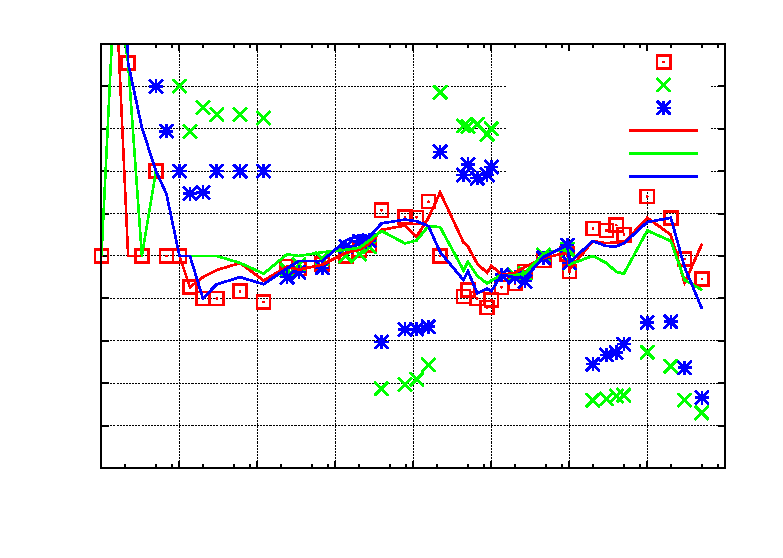
\includegraphics{../GNU/m328pres_all}}%
    \gplfronttext
  \end{picture}%
\endgroup
}
    \caption{mit drei ATmega328P}
    \label{fig:m328pres_all}
  \end{subfigure}
\caption{Relativer Fehler für Widerstands-Messungen}
\end{figure}


 \section{Messen von Kondensatoren}
Die Messung von Kapazitätswerten wird nach allen anderen Messungen als separater Teil mit einer Ladezeitmessung 
durchgeführt.
Die Originalsoftware vom Markus F. hat das mit einer Programmschleife gemacht, die den betreffenden digitalen
Eingangs-Pin bis zu einer Signaländerung gelesen hat und dabei die Schleifendurchläufe gezählt.
Dies hat den Nachteil, dass die Auflösung der Zeitmessung begrenzt ist durch die Gesamtzeit eines Schleifendurchlaufs.
Dies wurde üblicherweise in allen sechs Kombinationsmöglichkeiten für die drei Testpins durchgeführt.
Die aktuelle Software benutzt zwei verschiedene Möglichkeiten, um die Ladezeit in nur drei
Kombinationsmöglichkeiten für die drei Testpins zu erhalten.
Die positive Seite ist nun immer die höhere Testpin-Nummer.
Nur wenn die Kapazität zusammen mit einer parallel geschalteten Diode gemessen wird,
kann die Polarität die andere Richtung haben.

\subsection{Entladen der Kondensatoren}
Sie sollten die Kapazitäten immer entladen, bevor sie mit dem Tester verbunden werden.
Bevor irgendein Test gestartet wird, wird der Kondensator vom Tester immer noch einmal entladen.
Wenn die Spannung unter 1300mV ist, wird der Kondensator dafür mit den angeschlossenen ADC-Ports (Port C) kurzgeschlossen.
Ich glaube das ist in Ordnung, weil jeder Portausgang einen Innenwiderstand von ungefähr \(20\Omega\) hat.
Die Abbildung 149 (Seite 258) im Atmega8-Datenblatt \cite{ATmega8} zeigt einen Spannungsabfall an Ausgabe-Pins von bis zu 2V.
Natürlich kann ich nicht garantieren, dass kein Schaden auftreten kann.
Ich habe die Funktion mit Kondensatoren von mehr als \(15 mF\) sehr oft getestet und ich habe noch nie ein Problem bemerkt.
Der Strom sollte unter der spezifizierten Grenze von 40mA bleiben und reduziert sich schnell durch die Entladung.
Natürlich kann ein Schaden entstehen, wenn Sie einen (Hochvolt-) Kondensator nicht vollständig entladen, bevor Sie ihn an den Tester anschließen.

\subsection{Messung von großen Kapazitäten}
\label{sec:bigcap}
Eine Seite des Kondensators ist mit GND verbunden. Die andere Seite wird über den \(680\Omega\)-Widerstand für 10ms mit VCC verbunden.
Danach wird dieser Messpin auf Eingang geschaltet (hochohmig).
Nach diesem Strompuls wird die Spannung am Kondensator stromlos gemessen.
Wenn die Spannung noch nicht den Minimalwert von 300mV erreicht hat, wird dieser Ladepuls bis zu weiteren 499 Mal wiederholt.
Wenn nach 127 Pulsen (ungefähr 2s) noch nicht eine Minimalspannung von 75mV erreicht ist, wird der Ladevorgang abgebrochen,
 weil die 300mV mit den verbleibenden Ladepulsen nie erreicht werden wird.
Abbildung~\ref{fig:bigcap1} zeigt die drei Phasen der Kapazitätsbestimmung eines Kondensators.
Der Kapazitätswert wird dann berechnet aus der Ladepuls-Anzahl und der erreichten Ladespannung über eine Tabelle.
Die Tabelle enthält mit einem Spannungsabstand von 25mV die Faktoren, um aus der Ladezeit und der Spannung 
den Kapazitätswert zu bestimmen. 
Zwischenwerte der Spannung werden interpoliert.

\begin{figure}[H]
\centering

\includegraphics[]{../FIG/Bigcap.eps}
\caption{Kondensator-Entladung und -Ladung mit 10ms Ladepulsen bis zur Spannung \textgreater 300mV}
\label{fig:bigcap1}
\end{figure}

Wegen der niedrigen Ladespannung wird die Messung viel schneller als bei der ursprünglichen Softwareversion,
weil dieser Vorteil auch bei der Entladung wirkt. So können auch grössere Kondensatoren gemessen werden.
Zusätzlich stört in den meisten Fällen eine parallel geschaltete Diode nicht die Messung, weil die Schwellspannung
der Diode nicht erreicht wird.
Abbildung~\ref{pic:c229} zeigt das Laden und Entladen eines \(229\mu F\) großen Kondensators.
Das flache Dach der Messkurve bis zum Entladebeginn ist durch die Messzeit und Berechnungszeit des ATmega verursacht.
Abbildung~\ref{pic:c5mF} zeigt die gleiche Messung mit einem~\(5mF\)-Kondensator,
beachte wie die Messzeit inklusive Entladung auf ungefähr 1,5 Sekunden angewachsen ist.
Das letzte Beispiel in Abbildung~\ref{pic:c15mF} zeigt die Messung eines \(15mF\)-Kondensators.

\begin{figure}[H]
  \begin{subfigure}[b]{9cm}
    \centering
    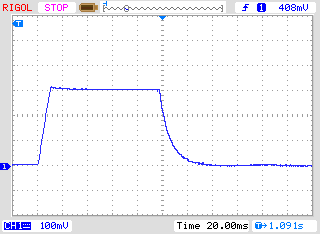
\includegraphics[width=9cm]{../PNG/charge_229uF.png}
    \caption{\(229\mu F\)-Kondensator}
    \label{pic:c229}
  \end{subfigure}
  ~
  \begin{subfigure}[b]{9cm}
    \centering
    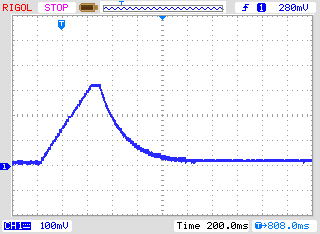
\includegraphics[width=9cm]{../PNG/charge_5mF.png}
    \caption{\(5mF\)-Kondensator}
    \label{pic:c5mF}
  \end{subfigure}
  \caption{Laden und Entladen von großen Kondensatoren für die Messung}
\end{figure}

\begin{figure}[H]
  \centering
    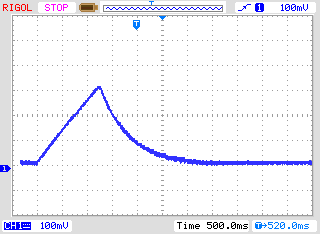
\includegraphics[]{../PNG/charge_15mF.png}
  \caption{Laden und Entladen eines \(15mF\)-Kondensators für die Messung}
  \label{pic:c15mF}
\end{figure}

Nach dieser Kondensatormessung wird die Selbstentladung des Kondensators untersucht, indem der
Spannungsverlust in einer der Ladezeit proportionalen Zeit untersucht wird.
Der gemessene Kapazitätswert wird entsprechend korrigiert. Ein Test mit einer Parallelschaltung von
einem \(68 \mu F\)-Kondensator mit einem \(2.2 k\Omega\)-Widerstand zeigt die
Wirksamkeit der Methode. Der ermittelte Kapazitätswert ohne den Widerstand beträgt \(66.5 \mu F\),
mit dem parallelen \(2.2 k\Omega\) Widerstand wird ein Kapazitätswert von \(65.3 \mu F\) gemessen.
Zum Vergleich möchte ich die entsprechenden Ergebnisse mit einem Peaktech 3315 Multimeter angeben.
Ohne den Widerstand wird eine Kapazität von \(68.2 \mu F\) gemessen, mit dem parallelen \(2.2 k\Omega\)
Widerstand wird aber \(192 \mu F\) mit dem Multimeter gemessen.

\subsection{Messen von kleinen Kapazitäten}
Wenn der erste 10 ms Ladepuls den Kondensator zu hoch aufgeladen hat, wird eine andere Messtechnik benutzt.
Der ATmega-Mikrocontroller hat einen eingebauten 16-Bit-Zähler, der bei voller Taktfrequenz (1MHz oder 8MHz) arbeiten kann.
Diese Zähler hat auch die Fähigkeit aufgrund eines externen Ereignisses den Zählerstand zu sichern.
Dieses Ereignis kann auch das Ausgangs-Signal des Komparators sein.
Der Komparator kann mit jedem ADC-Eingangspin und der Spannungsreferenz (Band Gap Reference) arbeiten.
Das Schaltbild~\ref{fig:comparat} zeigt ein vereinfachtes Diagram der Messsituation.
So entlade ich den Kondensator, bereite den Komparator für den richtigen Pin Eingang vor, starte den Zähler bei 0 und
starte sofort das Laden des Kondensators.
Dabei ist eine Seite des Kondensators mit GND, die andere Seite über den \(470k\Omega\)-Widerstand mit VCC verbunden.
Nun prüfe ich in einer Programm-Schleife, ob der Zähler ein Überlauf-Ereignis (overflow) oder ein
 externes Ereignis (input capture) meldet.
Die Überlauf-Ereignisse zähle ich, bis ich ein externes Ereignis feststelle.
In diesem Fall halte ich den Zähler an und prüfe, ob ich noch einen zusätzlichen Überlauf zählen muss, 
weil der Zähler nicht mit dem externen Ereignis (input capture) angehalten werden kann.


Der Zählerstand des externen Ereignisses bildet zusammen mit dem Überlaufzähler die Gesamtzeit, aus der die
Kapazität mit einem Faktor bestimmt wird.
Die aktuelle Software kann eine Tabelle mit der theoretischen Abhängigkeit der Ladezeit in Bezug auf die gemessene
Komparator-Spannung berücksichtigen.
Die Tabelle besitzt Einträge in Schritten von 50mV, die Ergebnisse werden entsprechend der aktuellen Referenz-Spannung interpoliert.
Diese Tabelle wird nur mit der Makefile Option WITH\_AUTO\_REF aktiviert.
Vom Kapazitätswert ziehe ich eine experimentell herausgefundene vordefinierte Konstante oder eine im Selbsttest
herausgefundene Konstante ab, um den Messwerte-Offset zu beseitigen.
Ich weiß nicht, ob die vordefinierte Konstante für andere Leiterplatten angepasst werden muss.
Mit einem Selbsttest bei gesetzter AUTO\_CAL Option wird diese Anpassung automatisch erledigt.

Ich habe bemerkt, dass die Referenz-Spannung meistens etwas zu klein gemessen wird,
 deshalb kann man einen Zusatz mit der Makefile Option REF\_C\_KORR angeben.
Nach der Kalibration mit der AUTO\_CAL option ist der REF\_C\_KORR Wert nur ein Zusatz zu der automatisch
gefundenen Differenz zwischen geladener Kondensator-Spannung und der internen Referenz-Spannung.
Die gemessene Referenz-Spannung wird dann mit dem Korrekturwert (in mV) korrigiert (addiert).
Wenn die Option WITH\_AUTO\_REF nicht benutzt wird, werden die Referenz-Spannungen entsprechend den Angaben in den
Datenblättern ~\cite{ATmega8}~\cite{ATmega168} der ATmega8, ATmega168 und ATmega328 berücksichtigt.
Eine Beispielmessung von diesem Typ ist in Abbildung~\ref{pic:c22uF} dargestellt.
Die Messzeit für den \(22 \mu F\)-Kondensator beträgt ungefähr 2,6s weil der \(470k\Omega\)-Widerstand für das Laden benutzt wird.
Aber das Entladen geht in diesem Fall viel schneller als das Laden.

\begin{figure}[H]
\centering

\includegraphics[]{../FIG/Comparat.eps}
\caption{Messung kleiner Kapazitätswerte mit dem Komparator}
\label{fig:comparat}
\end{figure}

\begin{figure}[H]
  \centering
    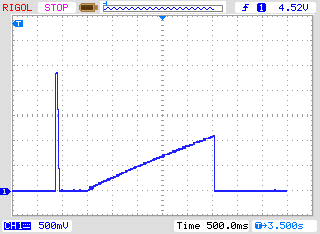
\includegraphics[]{../PNG/charge_22uF.png}
  \caption{Laden und Entladen eines \(22\mu F\)-Kondensators für die Messung}
  \label{pic:c22uF}
\end{figure}


Im Prinzip kann diese Technik auch mit dem \(680\Omega\)-Widerstand benutzt werden,
aber weil während dem Komparatorbetrieb der ADC nicht benutzt werden kann, besteht keine
Möglichkeit die Ladespannung zu beobachten bis der Komparator angehalten wird.
Wenn eine unentdeckte Diode mit dem Kondensator parallelgeschaltet ist, kann der Ladestrom
von der Diode aufgenommen werden (Schwellspannung) und die Referenz-Spannung würde nie erreicht.
Dieser Konzeptfehler wird mit der Methode vermieden, die in der aktuellen Software für große Kondensatoren in Kapitel~\ref{sec:bigcap}
verwendet wird.

\subsection{Messen des äquivalenten Serienwiderstandes ESR}
Der ESR \cite{ESR} stellt zum Beispiel ein Maß für die Alterung von Elektrolyt-Kondensatoren dar.
Die Abbildung~\ref{fig:Cap_equiv} zeigt ein Ersatzschaltbild eines Kondensators.
Der Widerstand \(Rp\) stellt den Isolationswiderstand des Kondensators dar, \(ESL\) die äquivalente
Serieninduktivität und der Widerstand \(ESR\) stellt den äquivalenten Serienwiderstand dar.

\begin{figure}[H]
  \centering
    \includegraphics[]{../FIG/Cap_equiv.eps}
  \caption{Ersatzschaltbild eines Kondensators}
  \label{fig:Cap_equiv}
\end{figure}

Es ist in Datenblättern üblich, den ESR gemessen bei einer Frequenz von 100 kHz und
einer Temperatur von \(20\textdegree C\) anzugeben.
Die Abbildungen \ref{fig:Cap_FC_data} und \ref{fig:Cap_FR_data} zeigen die vom Hersteller Panasonic 
angegebenen ESR Werte für die Elektrolytkondensatoren verschiedener Betriebs-Spannungen für die FC und die ,,low ESR'' FR Reihe.
Beide Serien sind für eine maximale Temperatur von \(105\textdegree C\) ausgelegt.
Die Abbildung \ref{fig:Cap_FC_FR_data} stellt die angegebenen Daten beider Serien bei einer zulässigen Betriebsspannung
von 25V dar. Wenn in der Baureihe verschiedene Ausführungen mit gleicher Kapazität und Spannung zur Verfügung stehen,
werden die Daten mit dem niedrigsten ESR dargestellt.
Bei Elektrolytkondensatoren sind sowohl der ESR Wert als auch die Kapazität relativ stark von der Betriebstemperatur
abhängig.

\begin{figure}[H]
  \centering
    \resizebox{14cm}{!}{% GNUPLOT: LaTeX picture with Postscript
\begingroup
  \makeatletter
  \providecommand\color[2][]{%
    \GenericError{(gnuplot) \space\space\space\@spaces}{%
      Package color not loaded in conjunction with
      terminal option `colourtext'%
    }{See the gnuplot documentation for explanation.%
    }{Either use 'blacktext' in gnuplot or load the package
      color.sty in LaTeX.}%
    \renewcommand\color[2][]{}%
  }%
  \providecommand\includegraphics[2][]{%
    \GenericError{(gnuplot) \space\space\space\@spaces}{%
      Package graphicx or graphics not loaded%
    }{See the gnuplot documentation for explanation.%
    }{The gnuplot epslatex terminal needs graphicx.sty or graphics.sty.}%
    \renewcommand\includegraphics[2][]{}%
  }%
  \providecommand\rotatebox[2]{#2}%
  \@ifundefined{ifGPcolor}{%
    \newif\ifGPcolor
    \GPcolortrue
  }{}%
  \@ifundefined{ifGPblacktext}{%
    \newif\ifGPblacktext
    \GPblacktexttrue
  }{}%
  % define a \g@addto@macro without @ in the name:
  \let\gplgaddtomacro\g@addto@macro
  % define empty templates for all commands taking text:
  \gdef\gplbacktext{}%
  \gdef\gplfronttext{}%
  \makeatother
  \ifGPblacktext
    % no textcolor at all
    \def\colorrgb#1{}%
    \def\colorgray#1{}%
  \else
    % gray or color?
    \ifGPcolor
      \def\colorrgb#1{\color[rgb]{#1}}%
      \def\colorgray#1{\color[gray]{#1}}%
      \expandafter\def\csname LTw\endcsname{\color{white}}%
      \expandafter\def\csname LTb\endcsname{\color{black}}%
      \expandafter\def\csname LTa\endcsname{\color{black}}%
      \expandafter\def\csname LT0\endcsname{\color[rgb]{1,0,0}}%
      \expandafter\def\csname LT1\endcsname{\color[rgb]{0,1,0}}%
      \expandafter\def\csname LT2\endcsname{\color[rgb]{0,0,1}}%
      \expandafter\def\csname LT3\endcsname{\color[rgb]{1,0,1}}%
      \expandafter\def\csname LT4\endcsname{\color[rgb]{0,1,1}}%
      \expandafter\def\csname LT5\endcsname{\color[rgb]{1,1,0}}%
      \expandafter\def\csname LT6\endcsname{\color[rgb]{0,0,0}}%
      \expandafter\def\csname LT7\endcsname{\color[rgb]{1,0.3,0}}%
      \expandafter\def\csname LT8\endcsname{\color[rgb]{0.5,0.5,0.5}}%
    \else
      % gray
      \def\colorrgb#1{\color{black}}%
      \def\colorgray#1{\color[gray]{#1}}%
      \expandafter\def\csname LTw\endcsname{\color{white}}%
      \expandafter\def\csname LTb\endcsname{\color{black}}%
      \expandafter\def\csname LTa\endcsname{\color{black}}%
      \expandafter\def\csname LT0\endcsname{\color{black}}%
      \expandafter\def\csname LT1\endcsname{\color{black}}%
      \expandafter\def\csname LT2\endcsname{\color{black}}%
      \expandafter\def\csname LT3\endcsname{\color{black}}%
      \expandafter\def\csname LT4\endcsname{\color{black}}%
      \expandafter\def\csname LT5\endcsname{\color{black}}%
      \expandafter\def\csname LT6\endcsname{\color{black}}%
      \expandafter\def\csname LT7\endcsname{\color{black}}%
      \expandafter\def\csname LT8\endcsname{\color{black}}%
    \fi
  \fi
  \setlength{\unitlength}{0.0500bp}%
  \begin{picture}(7200.00,5040.00)%
    \gplgaddtomacro\gplbacktext{%
      \csname LTb\endcsname%
      \put(1078,704){\makebox(0,0)[r]{\strut{} 0.01}}%
      \csname LTb\endcsname%
      \put(1078,2061){\makebox(0,0)[r]{\strut{} 0.1}}%
      \csname LTb\endcsname%
      \put(1078,3418){\makebox(0,0)[r]{\strut{} 1}}%
      \csname LTb\endcsname%
      \put(1078,4775){\makebox(0,0)[r]{\strut{} 10}}%
      \csname LTb\endcsname%
      \put(1210,484){\makebox(0,0){\strut{} 1}}%
      \csname LTb\endcsname%
      \put(2307,484){\makebox(0,0){\strut{} 10}}%
      \csname LTb\endcsname%
      \put(3403,484){\makebox(0,0){\strut{} 100}}%
      \csname LTb\endcsname%
      \put(4500,484){\makebox(0,0){\strut{} 1000}}%
      \csname LTb\endcsname%
      \put(5596,484){\makebox(0,0){\strut{} 10000}}%
      \csname LTb\endcsname%
      \put(6693,484){\makebox(0,0){\strut{} 100000}}%
      \put(176,2739){\rotatebox{-270}{\makebox(0,0){\strut{}ESR / Ohm}}}%
      \put(6912,2739){\rotatebox{-270}{\makebox(0,0){\strut{}}}}%
      \put(3951,154){\makebox(0,0){\strut{}Capacity / uF}}%
      \put(3951,4665){\makebox(0,0){\strut{}}}%
      \put(3951,4664){\makebox(0,0){\strut{}}}%
      \put(286,110){\makebox(0,0)[l]{\strut{}}}%
    }%
    \gplgaddtomacro\gplfronttext{%
      \csname LTb\endcsname%
      \put(5706,4602){\makebox(0,0)[r]{\strut{}6V}}%
      \csname LTb\endcsname%
      \put(5706,4382){\makebox(0,0)[r]{\strut{}16V}}%
      \csname LTb\endcsname%
      \put(5706,4162){\makebox(0,0)[r]{\strut{}35V}}%
      \csname LTb\endcsname%
      \put(5706,3942){\makebox(0,0)[r]{\strut{}63V}}%
    }%
    \gplbacktext
    \put(0,0){\includegraphics{../GNU/Cap_FC_data}}%
    \gplfronttext
  \end{picture}%
\endgroup
}
  \caption{ESR-Werte aus dem Panasonic Datenblatt der Serie FC}
  \label{fig:Cap_FC_data}
\end{figure}

\begin{figure}[H]
  \centering
    \resizebox{14cm}{!}{% GNUPLOT: LaTeX picture with Postscript
\begingroup
  \makeatletter
  \providecommand\color[2][]{%
    \GenericError{(gnuplot) \space\space\space\@spaces}{%
      Package color not loaded in conjunction with
      terminal option `colourtext'%
    }{See the gnuplot documentation for explanation.%
    }{Either use 'blacktext' in gnuplot or load the package
      color.sty in LaTeX.}%
    \renewcommand\color[2][]{}%
  }%
  \providecommand\includegraphics[2][]{%
    \GenericError{(gnuplot) \space\space\space\@spaces}{%
      Package graphicx or graphics not loaded%
    }{See the gnuplot documentation for explanation.%
    }{The gnuplot epslatex terminal needs graphicx.sty or graphics.sty.}%
    \renewcommand\includegraphics[2][]{}%
  }%
  \providecommand\rotatebox[2]{#2}%
  \@ifundefined{ifGPcolor}{%
    \newif\ifGPcolor
    \GPcolortrue
  }{}%
  \@ifundefined{ifGPblacktext}{%
    \newif\ifGPblacktext
    \GPblacktexttrue
  }{}%
  % define a \g@addto@macro without @ in the name:
  \let\gplgaddtomacro\g@addto@macro
  % define empty templates for all commands taking text:
  \gdef\gplbacktext{}%
  \gdef\gplfronttext{}%
  \makeatother
  \ifGPblacktext
    % no textcolor at all
    \def\colorrgb#1{}%
    \def\colorgray#1{}%
  \else
    % gray or color?
    \ifGPcolor
      \def\colorrgb#1{\color[rgb]{#1}}%
      \def\colorgray#1{\color[gray]{#1}}%
      \expandafter\def\csname LTw\endcsname{\color{white}}%
      \expandafter\def\csname LTb\endcsname{\color{black}}%
      \expandafter\def\csname LTa\endcsname{\color{black}}%
      \expandafter\def\csname LT0\endcsname{\color[rgb]{1,0,0}}%
      \expandafter\def\csname LT1\endcsname{\color[rgb]{0,1,0}}%
      \expandafter\def\csname LT2\endcsname{\color[rgb]{0,0,1}}%
      \expandafter\def\csname LT3\endcsname{\color[rgb]{1,0,1}}%
      \expandafter\def\csname LT4\endcsname{\color[rgb]{0,1,1}}%
      \expandafter\def\csname LT5\endcsname{\color[rgb]{1,1,0}}%
      \expandafter\def\csname LT6\endcsname{\color[rgb]{0,0,0}}%
      \expandafter\def\csname LT7\endcsname{\color[rgb]{1,0.3,0}}%
      \expandafter\def\csname LT8\endcsname{\color[rgb]{0.5,0.5,0.5}}%
    \else
      % gray
      \def\colorrgb#1{\color{black}}%
      \def\colorgray#1{\color[gray]{#1}}%
      \expandafter\def\csname LTw\endcsname{\color{white}}%
      \expandafter\def\csname LTb\endcsname{\color{black}}%
      \expandafter\def\csname LTa\endcsname{\color{black}}%
      \expandafter\def\csname LT0\endcsname{\color{black}}%
      \expandafter\def\csname LT1\endcsname{\color{black}}%
      \expandafter\def\csname LT2\endcsname{\color{black}}%
      \expandafter\def\csname LT3\endcsname{\color{black}}%
      \expandafter\def\csname LT4\endcsname{\color{black}}%
      \expandafter\def\csname LT5\endcsname{\color{black}}%
      \expandafter\def\csname LT6\endcsname{\color{black}}%
      \expandafter\def\csname LT7\endcsname{\color{black}}%
      \expandafter\def\csname LT8\endcsname{\color{black}}%
    \fi
  \fi
  \setlength{\unitlength}{0.0500bp}%
  \begin{picture}(7200.00,5040.00)%
    \gplgaddtomacro\gplbacktext{%
      \csname LTb\endcsname%
      \put(1078,704){\makebox(0,0)[r]{\strut{} 0.01}}%
      \csname LTb\endcsname%
      \put(1078,2740){\makebox(0,0)[r]{\strut{} 0.1}}%
      \csname LTb\endcsname%
      \put(1078,4775){\makebox(0,0)[r]{\strut{} 1}}%
      \csname LTb\endcsname%
      \put(1210,484){\makebox(0,0){\strut{} 10}}%
      \csname LTb\endcsname%
      \put(3074,484){\makebox(0,0){\strut{} 100}}%
      \csname LTb\endcsname%
      \put(4939,484){\makebox(0,0){\strut{} 1000}}%
      \csname LTb\endcsname%
      \put(6803,484){\makebox(0,0){\strut{} 10000}}%
      \put(176,2739){\rotatebox{-270}{\makebox(0,0){\strut{}ESR / Ohm}}}%
      \put(4006,154){\makebox(0,0){\strut{}Capacity / uF}}%
      \put(4006,4665){\makebox(0,0){\strut{}}}%
      \put(4006,4664){\makebox(0,0){\strut{}}}%
      \put(286,110){\makebox(0,0)[l]{\strut{}}}%
    }%
    \gplgaddtomacro\gplfronttext{%
      \csname LTb\endcsname%
      \put(5816,4602){\makebox(0,0)[r]{\strut{}6V}}%
      \csname LTb\endcsname%
      \put(5816,4382){\makebox(0,0)[r]{\strut{}16V}}%
      \csname LTb\endcsname%
      \put(5816,4162){\makebox(0,0)[r]{\strut{}35V}}%
      \csname LTb\endcsname%
      \put(5816,3942){\makebox(0,0)[r]{\strut{}63V}}%
    }%
    \gplbacktext
    \put(0,0){\includegraphics{../GNU/Cap_FR_data}}%
    \gplfronttext
  \end{picture}%
\endgroup
}
  \caption{ESR-Werte aus dem Panasonic Datenblatt der Serie FR}
  \label{fig:Cap_FR_data}
\end{figure}

\begin{figure}[H]
  \centering
    \resizebox{14cm}{!}{% GNUPLOT: LaTeX picture with Postscript
\begingroup
  \makeatletter
  \providecommand\color[2][]{%
    \GenericError{(gnuplot) \space\space\space\@spaces}{%
      Package color not loaded in conjunction with
      terminal option `colourtext'%
    }{See the gnuplot documentation for explanation.%
    }{Either use 'blacktext' in gnuplot or load the package
      color.sty in LaTeX.}%
    \renewcommand\color[2][]{}%
  }%
  \providecommand\includegraphics[2][]{%
    \GenericError{(gnuplot) \space\space\space\@spaces}{%
      Package graphicx or graphics not loaded%
    }{See the gnuplot documentation for explanation.%
    }{The gnuplot epslatex terminal needs graphicx.sty or graphics.sty.}%
    \renewcommand\includegraphics[2][]{}%
  }%
  \providecommand\rotatebox[2]{#2}%
  \@ifundefined{ifGPcolor}{%
    \newif\ifGPcolor
    \GPcolortrue
  }{}%
  \@ifundefined{ifGPblacktext}{%
    \newif\ifGPblacktext
    \GPblacktexttrue
  }{}%
  % define a \g@addto@macro without @ in the name:
  \let\gplgaddtomacro\g@addto@macro
  % define empty templates for all commands taking text:
  \gdef\gplbacktext{}%
  \gdef\gplfronttext{}%
  \makeatother
  \ifGPblacktext
    % no textcolor at all
    \def\colorrgb#1{}%
    \def\colorgray#1{}%
  \else
    % gray or color?
    \ifGPcolor
      \def\colorrgb#1{\color[rgb]{#1}}%
      \def\colorgray#1{\color[gray]{#1}}%
      \expandafter\def\csname LTw\endcsname{\color{white}}%
      \expandafter\def\csname LTb\endcsname{\color{black}}%
      \expandafter\def\csname LTa\endcsname{\color{black}}%
      \expandafter\def\csname LT0\endcsname{\color[rgb]{1,0,0}}%
      \expandafter\def\csname LT1\endcsname{\color[rgb]{0,1,0}}%
      \expandafter\def\csname LT2\endcsname{\color[rgb]{0,0,1}}%
      \expandafter\def\csname LT3\endcsname{\color[rgb]{1,0,1}}%
      \expandafter\def\csname LT4\endcsname{\color[rgb]{0,1,1}}%
      \expandafter\def\csname LT5\endcsname{\color[rgb]{1,1,0}}%
      \expandafter\def\csname LT6\endcsname{\color[rgb]{0,0,0}}%
      \expandafter\def\csname LT7\endcsname{\color[rgb]{1,0.3,0}}%
      \expandafter\def\csname LT8\endcsname{\color[rgb]{0.5,0.5,0.5}}%
    \else
      % gray
      \def\colorrgb#1{\color{black}}%
      \def\colorgray#1{\color[gray]{#1}}%
      \expandafter\def\csname LTw\endcsname{\color{white}}%
      \expandafter\def\csname LTb\endcsname{\color{black}}%
      \expandafter\def\csname LTa\endcsname{\color{black}}%
      \expandafter\def\csname LT0\endcsname{\color{black}}%
      \expandafter\def\csname LT1\endcsname{\color{black}}%
      \expandafter\def\csname LT2\endcsname{\color{black}}%
      \expandafter\def\csname LT3\endcsname{\color{black}}%
      \expandafter\def\csname LT4\endcsname{\color{black}}%
      \expandafter\def\csname LT5\endcsname{\color{black}}%
      \expandafter\def\csname LT6\endcsname{\color{black}}%
      \expandafter\def\csname LT7\endcsname{\color{black}}%
      \expandafter\def\csname LT8\endcsname{\color{black}}%
    \fi
  \fi
  \setlength{\unitlength}{0.0500bp}%
  \begin{picture}(7200.00,5040.00)%
    \gplgaddtomacro\gplbacktext{%
      \csname LTb\endcsname%
      \put(1078,704){\makebox(0,0)[r]{\strut{} 0.01}}%
      \csname LTb\endcsname%
      \put(1078,2061){\makebox(0,0)[r]{\strut{} 0.1}}%
      \csname LTb\endcsname%
      \put(1078,3418){\makebox(0,0)[r]{\strut{} 1}}%
      \csname LTb\endcsname%
      \put(1078,4775){\makebox(0,0)[r]{\strut{} 10}}%
      \csname LTb\endcsname%
      \put(1210,484){\makebox(0,0){\strut{} 10}}%
      \csname LTb\endcsname%
      \put(3074,484){\makebox(0,0){\strut{} 100}}%
      \csname LTb\endcsname%
      \put(4939,484){\makebox(0,0){\strut{} 1000}}%
      \csname LTb\endcsname%
      \put(6803,484){\makebox(0,0){\strut{} 10000}}%
      \put(176,2739){\rotatebox{-270}{\makebox(0,0){\strut{}ESR / Ohm}}}%
      \put(4006,154){\makebox(0,0){\strut{}Capacity / uF}}%
      \put(4006,4665){\makebox(0,0){\strut{}}}%
      \put(286,110){\makebox(0,0)[l]{\strut{}}}%
    }%
    \gplgaddtomacro\gplfronttext{%
      \csname LTb\endcsname%
      \put(5816,4602){\makebox(0,0)[r]{\strut{}FC 25V}}%
      \csname LTb\endcsname%
      \put(5816,4382){\makebox(0,0)[r]{\strut{}FR 25V}}%
    }%
    \gplbacktext
    \put(0,0){\includegraphics{../GNU/Cap_FC_FR_data}}%
    \gplfronttext
  \end{picture}%
\endgroup
}
  \caption{Vergleich der ESR-Werte der Serie FC mit der Serie FR}
  \label{fig:Cap_FC_FR_data}
\end{figure}

Eine Messung bei 100 kHz ist mit der Hardware des ATmega nicht ohne weiteres möglich, da weder der ADC
eine direkte Abtastung einer so hohen Eingangsfrequenz zuläßt, noch ein 100 kHz Signal bei der vorhandenen Schaltung zur
Verfügung steht. 
Als nächstes werden hier zwei Methoden für die Bestimmung des ESR vorgestellt, die mit der vohandenen
Schaltung auskommen. 
Beide Methoden verwenden für die Messung ein rechteckförmiges Meßsignal, so daß die Ergebnisse nie
exakt mit den Angaben übereinstimmen können, die bei einem sinus-förmigen Signal gemessen werden.
Bei der ersten Methode liegen die Ergebnisse nahe bei den ESR-Werten, die bei 1 kHz ermittelt werden.
Die zweite Methode hat aber den Vorteil, daß der Nullwert mit kurzgeschlossenen Testpins ermittelt werden kann
und daß zusätzlich der ermittelte ESR sich dem bei 10 kHz Meßfrequenz gemessenen Wert nähert.
Ich habe derzeit keine Idee für eine Meßmethode, die einen direkt zu der 100 kHz Messung einen 
vergleichbaren ESR-Wert liefern kann.

Die folgende Tabelle \ref{tab:capESR} soll die Abhängigkeit des ESR von der Frequenz zeigen.
Außer dem \(47 \mu F\) Kondensator sind alle Kondensatoren aus der Baureihe FC von Panasonic.
Die Referenzwerte wurden mit einem Peaktech 2170 LCR-Meßgerät ermittelt.
Alle TransistorTester Resultate in dieser Tabelle wurden mit der im Unterkapitel \ref{sec:ESR2} 
beschriebenen Methode 2 gemessen.
Bei großen Kapazitätswerten macht die ebenfalls vorhandene Induktivität ESL das Messen bei höheren Frequenzen 
wie 100 kHz schwierig.


\begin{table}[H]
  \begin{center}
    \begin{tabular}{| l | c | c | c | c | c |}
   \hline
            & Datenblatt & PeakTech  & Peaktech & PeakTech & Transistor- \\
Kondensator & 100 kHz    & 100 kHz   & 10 kHz   & 1 kHz    & tester  \\
    \hline
    \hline
1uF / 50V    & 2.4       & 1.27      & 1.75     & 4.31     &  2.1 \\
    \hline
2.2uF / 50V  & 1.8       & 1.07      & 1.34     & 2.76     &  1.6 \\
    \hline
4.7uF / 50V  & 1.3       & 1.19      & 1.40     & 2.37     &  1.5 \\
    \hline
4.7uF / 50V  & 1.3       & 1.19      & 1.40     & 2.37     &  1.5 \\
    \hline
10uF / 50V   & 1.3       & 1.26      & 1.45     & 2.05     &  1.5 \\
    \hline
22uF / 10V   & 2.0       & 1.52      & 1.76     & 2.24     &  1.9 \\
    \hline
47uF / 63V   & ?         & 0.46      & 0.50     & 0.63     &  0.52 \\
    \hline
    \end{tabular}
  \end{center}
  \caption{ESR-Werte verschiedener Elektrolyt-Kondensatoren}
  \label{tab:capESR} 
\end{table}


\subsection{Messen des äquivalenten Serienwiderstandes ESR, Methode 1}
Bei Kondensatoren mit mehr als \(0.45 \mu F\) wird versucht, den Serienwiderstand von Kondensatoren zu messen.
Bei mehr als \(3.6 \mu F\) wird dazu die normale Taktrate von \(125 kHz\) für den Analog-Digital Wandler benutzt.
Bei kleineren Kapazitäten wird eine erhöhte Taktrate von \(500 kHz\) benutzt, um die Messung zu beschleunigen.
Die Genauigkeit der ADC-Ergebnisse wird bei der höheren Taktrate zwar schlechter, aber die größeren ESR-Werte
bei kleineren Kondensatoren mildern die Auswirkung dieses Genauigkeitsverlusts ab. 
Andererseits ist sonst nach diesem Verfahren keine ESR-Messung für Kondensatoren unter \(1.8 \mu F\) möglich.

Genau genommen ist der ESR eines Kondensators abhängig von der Betriebsfrequenz und der Temperatur.
Üblicherweise wird der mit einem sinusförmigen Signal bei \(100 kHz\) gemessene Wert in Datenblättern angegeben.
Bei dieser Frequenz kann der ATmega ohne externe Beschaltung keine Messung durchführen.
Das nachfolgend beschriebene Verfahren erreicht bei der normalen ADC-Taktrate nur eine Messfrequenz von unter 640 Hz
 mit näherungsweise rechteckigem Signal. Bei \(500 kHz\) ADC Taktrate wird etwa 2400 Hz Meßfrequenz erreicht.
Um den äquivalenten Serienwiderstand zu bestimmen,
 wird der Kondensator zuerst in einer Richtung geladen und an beiden Anschlüssen die Spannung mit der internen
Referenzspannung (1.1 V) gemessen.
Nach der Messung wird der Ladestrom abgeschaltet und die Spannung am Kondensator ohne den
Ladestrom gemessen. Wenn die Spannung am Kondensator ohne Ladestrom weniger als 3 mV beträgt, wird
diese Messfolge wiederholt.
Die Abbildung~\ref{fig:Cap_esr} zeigt die entsprechenden Schaltungen.

\begin{figure}[H]
  \centering
    \includegraphics[]{../FIG/Cap_esr.eps}
  \caption{Schaltbild der ESR-Messung eines Kondensators}
  \label{fig:Cap_esr}
\end{figure}

Die Differenz der Spannung am Kondensator mit und ohne Strom ist ein Maß für den internen Widerstand des Kondensators.
Die zu erwartende Spannungsdifferenz ist allerdings so gering, dass mit einer Messung kein brauchbares Ergebnis erzielt
werden kann.
Aus diesem Grund wird danach der Strom umgekehrt und die Messung in der anderen Richtung wiederholt.
Die gesamte Mess-Sequenz wird 128 Mal durchgeführt und die Ergebnisse der Spannungsmessungen addiert.
Danach hat man drei Spannungssummen, die Spannung \(Ulp\) am Minuspol des Kondensators mit Strom, die Spannung \(Uhp\) am
Pluspol des Kondensators mit Strom und die Spannung \(Uc\) am Pluspol des Kondensators ohne Strom.
Die Spannungssumme am Minuspol des Kondensators repräsentiert den Spannungsabfall bei einem mittleren
Ladestrom am Port-Ausgangswiderstand \(Rport\). Aus der Differenz der Spannungssumme am Pluspol und Minuspol des Kondensators
hat man ein Maß für die Spannung am Kondensator mit Ladestrom \(Udiff = Uhp - Ulp\).
Die Differenz \(Uesr = Udiff - Uc\) soll jetzt den Spannungsabfall bei mittlerem Ladestrom am internen Widerstand des Kondensators
repräsentieren.
Der Widerstandswert wird aus dem Verhältnis dieser Spannung \(Uesr\) zu der Spannung \(Ulp\) skaliert mit dem
bekannten Widerstandwert des Port-Ausgangs \(Rport\). Dabei wird so skaliert, dass eine Widerstandauflösung von
\(0.01 \Omega\) erreicht wird \(Resr = \frac{Uesr \cdot 10 \cdot Rport}{Ulp}\).
Die Abbildung~\ref{pic:esr4} zeigt den Ausschnitt des Spannungsverlaufs eines \(4.2\mu F\) Kondensators
 während der ESR-Messung. Dem Kondensator wurde ein \(6.8 \Omega\) Widerstand in Serie geschaltet, um den ESR Einfluß
zu verdeutlichen. Der kleine Spannungseinbruch nach dem Ladevorgang des Kondensators wird von der Software ausgewertet.
Der größere Spannungseinbruch bei der Messung gegen GND kommt durch den Einfluß des Port-Ausgangswiderstands von etwa \(20 \Omega\) zustande.
Das Ergebnis der ESR-Messung ist in diesem Fall \(7.5 \Omega\), ohne den \(6.8 \Omega\) Widerstand sind es \(0.56 \Omega\).
Die Abbildung~\ref{pic:esr2} zeigt die gleiche Messung mit höherer Meßfrequenz bei einem \(2.2 \mu F\) Elko mit einem ESR von \(6.5 \Omega\).


\begin{figure}[H]
  \begin{subfigure}[b]{9cm}
    \centering
    \includegraphics[width=9cm]{../PNG/ESR_4uF.png}
    \caption{Ein Pin gegen GND gemessen}
  \end{subfigure}
  ~
  \begin{subfigure}[b]{9cm}
    \centering
    \includegraphics[width=9cm]{../PNG/ESR4uF6R8.png}
    \caption{Von Pin zu Pin gemessen}
  \end{subfigure}
  \caption{Spannungsverlauf eines \(4.2\mu F\) Kondensators während der ESR-Messung}
  \label{pic:esr4}
\end{figure}

\begin{figure}[H]
  \begin{subfigure}[b]{9cm}
    \centering
    \includegraphics[width=9cm]{../PNG/ESR_2uF_pin2GND.png}
    \caption{Ein Pin gegen GND gemessen}
  \end{subfigure}
  ~
  \begin{subfigure}[b]{9cm}
    \centering
    \includegraphics[width=9cm]{../PNG/ESR_2uF_pin2pin.png}
    \caption{Von Pin zu Pin gemessen}
  \end{subfigure}
  \caption{Spannungsverlauf eines \(2.2\mu F\) Kondensators während der ESR-Messung}
  \label{pic:esr2}
\end{figure}

Die Genauigkeit der ESR-Messung ist aus verschiedenen Gründen nicht sehr hoch:
\begin{enumerate}
\item Die Spannungsmessung an den beiden Kondensator-Anschlüssen kann nicht gleichzeitig sondern nur nacheinander durchgeführt werden.
 In der Zwischenzeit hat sich der Ladestrom durch den Ladevorgang des Kondensators geändert.
Dies wird versucht mit einer kapazitätsabhängigen Korrektur der Minuspol-Spannung auszugleichen.
\item Der ADC nimmt den Spannungswert 1,5 Takte nach dem Start des Wandlungsvorgangs. Der Wandelvorgang beginnt mit
der steigenden Flanke des ADC-Taktes, wenn das Startbit gesetzt ist. Wenn der Ladestrom des Kondensators zu früh abgeschaltet wird,
nimmt der ADC die falsche Spannung für die strombehaftete Messung auf. Wird der Ladestrom zu spät abgeschaltet, wird
der Kondensator weiter geladen als es der strombehafteten Messung entspricht.
Dann wird im stromlosen Zustand eine zu hohe Spannung gemessen.
Es ist aber schwierig im Programm den genauen Zeitpunkt für die Stromabschaltung zu treffen.
\item Der Port-Ausgangswiderstand wird bei dieser Messmethode als Referenz benutzt, dessen Widerstandwert
ist aber auch nicht exakt bekannt.
\item Die Auflösung des ADC reicht nicht aus, um eine Widerstandsauflösung von \(0.01 \Omega\) zu erreichen.
Für alle Messungen wird die interne Spannungsreferenz (1.1 V) benutzt, um die best mögliche Auflösung zu verwenden.
Zusätzlich wird versucht, den Auflösungs-Mangel durch eine große Zahl von Einzelmessungen abzumildern.
\item Mit der Abfrage des Fertig-Signals der ADC-Wandlung gelingt es nicht exakt, die Schaltzeiten der Port-Ausgänge mit dem
ADC-Takt zu synchronisieren.
\end{enumerate}

Trotz allen Schwierigkeiten scheinen die Ergebnisse brauchbar zu sein, wie die nachfolgende Abbildung \ref{fig:Cesr} zeigt.
Die ESR-Werte eines Bauteils gemessen mit dem Transistortester schwanken stärker als die Messungen des LCR-meters.
Die Messergebnisse des LCR-Messgerätes wurden bei einer Frequenz von 1 kHz gemessen oder für kleine Kapazitäten auf
2.4 kHz interpoliert.
Beim Transistortester muss auf die Qualität der Anschlüsse geachtet werden. Verwendete Anschlusskabel
erhöhen den gemessenen Widerstandswert. Auch die Kontakte von Steckverbindern können die gemessenen
Widerstandwerte erhöhen. Das LCR-Messgerät macht hier wegen den verwendeten Kelvin-Klemmen weniger Probleme.
Bei den Kondensatoren mit einer Kapazität unter \(1 \mu F\) war ein \(500 nF\) keramischer 
Kondensator (Z5U), alle anderen waren Folien-Kondensatoren. Der einzige Elektrolyt-Kondensator der Meßreihe unter \(9 \mu F\)  
ist ein \(2.2 \mu F\) Kondensator.

\begin{figure}[H]
\centering
% GNUPLOT: LaTeX picture with Postscript
\begingroup
  \makeatletter
  \providecommand\color[2][]{%
    \GenericError{(gnuplot) \space\space\space\@spaces}{%
      Package color not loaded in conjunction with
      terminal option `colourtext'%
    }{See the gnuplot documentation for explanation.%
    }{Either use 'blacktext' in gnuplot or load the package
      color.sty in LaTeX.}%
    \renewcommand\color[2][]{}%
  }%
  \providecommand\includegraphics[2][]{%
    \GenericError{(gnuplot) \space\space\space\@spaces}{%
      Package graphicx or graphics not loaded%
    }{See the gnuplot documentation for explanation.%
    }{The gnuplot epslatex terminal needs graphicx.sty or graphics.sty.}%
    \renewcommand\includegraphics[2][]{}%
  }%
  \providecommand\rotatebox[2]{#2}%
  \@ifundefined{ifGPcolor}{%
    \newif\ifGPcolor
    \GPcolortrue
  }{}%
  \@ifundefined{ifGPblacktext}{%
    \newif\ifGPblacktext
    \GPblacktexttrue
  }{}%
  % define a \g@addto@macro without @ in the name:
  \let\gplgaddtomacro\g@addto@macro
  % define empty templates for all commands taking text:
  \gdef\gplbacktext{}%
  \gdef\gplfronttext{}%
  \makeatother
  \ifGPblacktext
    % no textcolor at all
    \def\colorrgb#1{}%
    \def\colorgray#1{}%
  \else
    % gray or color?
    \ifGPcolor
      \def\colorrgb#1{\color[rgb]{#1}}%
      \def\colorgray#1{\color[gray]{#1}}%
      \expandafter\def\csname LTw\endcsname{\color{white}}%
      \expandafter\def\csname LTb\endcsname{\color{black}}%
      \expandafter\def\csname LTa\endcsname{\color{black}}%
      \expandafter\def\csname LT0\endcsname{\color[rgb]{1,0,0}}%
      \expandafter\def\csname LT1\endcsname{\color[rgb]{0,1,0}}%
      \expandafter\def\csname LT2\endcsname{\color[rgb]{0,0,1}}%
      \expandafter\def\csname LT3\endcsname{\color[rgb]{1,0,1}}%
      \expandafter\def\csname LT4\endcsname{\color[rgb]{0,1,1}}%
      \expandafter\def\csname LT5\endcsname{\color[rgb]{1,1,0}}%
      \expandafter\def\csname LT6\endcsname{\color[rgb]{0,0,0}}%
      \expandafter\def\csname LT7\endcsname{\color[rgb]{1,0.3,0}}%
      \expandafter\def\csname LT8\endcsname{\color[rgb]{0.5,0.5,0.5}}%
    \else
      % gray
      \def\colorrgb#1{\color{black}}%
      \def\colorgray#1{\color[gray]{#1}}%
      \expandafter\def\csname LTw\endcsname{\color{white}}%
      \expandafter\def\csname LTb\endcsname{\color{black}}%
      \expandafter\def\csname LTa\endcsname{\color{black}}%
      \expandafter\def\csname LT0\endcsname{\color{black}}%
      \expandafter\def\csname LT1\endcsname{\color{black}}%
      \expandafter\def\csname LT2\endcsname{\color{black}}%
      \expandafter\def\csname LT3\endcsname{\color{black}}%
      \expandafter\def\csname LT4\endcsname{\color{black}}%
      \expandafter\def\csname LT5\endcsname{\color{black}}%
      \expandafter\def\csname LT6\endcsname{\color{black}}%
      \expandafter\def\csname LT7\endcsname{\color{black}}%
      \expandafter\def\csname LT8\endcsname{\color{black}}%
    \fi
  \fi
  \setlength{\unitlength}{0.0500bp}%
  \begin{picture}(7200.00,5040.00)%
    \gplgaddtomacro\gplbacktext{%
      \csname LTb\endcsname%
      \put(682,704){\makebox(0,0)[r]{\strut{} 0}}%
      \csname LTb\endcsname%
      \put(682,1286){\makebox(0,0)[r]{\strut{} 1}}%
      \csname LTb\endcsname%
      \put(682,1867){\makebox(0,0)[r]{\strut{} 2}}%
      \csname LTb\endcsname%
      \put(682,2449){\makebox(0,0)[r]{\strut{} 3}}%
      \csname LTb\endcsname%
      \put(682,3030){\makebox(0,0)[r]{\strut{} 4}}%
      \csname LTb\endcsname%
      \put(682,3612){\makebox(0,0)[r]{\strut{} 5}}%
      \csname LTb\endcsname%
      \put(682,4193){\makebox(0,0)[r]{\strut{} 6}}%
      \csname LTb\endcsname%
      \put(682,4775){\makebox(0,0)[r]{\strut{} 7}}%
      \csname LTb\endcsname%
      \put(814,484){\makebox(0,0){\strut{}100n}}%
      \csname LTb\endcsname%
      \put(2311,484){\makebox(0,0){\strut{}1u}}%
      \csname LTb\endcsname%
      \put(3809,484){\makebox(0,0){\strut{}10u}}%
      \csname LTb\endcsname%
      \put(5306,484){\makebox(0,0){\strut{}100u}}%
      \csname LTb\endcsname%
      \put(6803,484){\makebox(0,0){\strut{}1m}}%
      \put(176,2739){\rotatebox{-270}{\makebox(0,0){\strut{}ESR / Ohm}}}%
      \put(3808,154){\makebox(0,0){\strut{}Capacity value / F}}%
      \put(3808,4665){\makebox(0,0){\strut{}}}%
    }%
    \gplgaddtomacro\gplfronttext{%
      \csname LTb\endcsname%
      \put(5690,4594){\makebox(0,0)[r]{\strut{}328p}}%
      \csname LTb\endcsname%
      \put(5690,4358){\makebox(0,0)[r]{\strut{}328}}%
      \csname LTb\endcsname%
      \put(5690,4122){\makebox(0,0)[r]{\strut{}168p}}%
      \csname LTb\endcsname%
      \put(5690,3886){\makebox(0,0)[r]{\strut{}168a}}%
      \csname LTb\endcsname%
      \put(5690,3650){\makebox(0,0)[r]{\strut{}168}}%
      \csname LTb\endcsname%
      \put(5690,3414){\makebox(0,0)[r]{\strut{}LCR}}%
    }%
    \gplbacktext
    \put(0,0){\includegraphics{../GNU/Cesr}}%
    \gplfronttext
  \end{picture}%
\endgroup

\caption{Messergebnisse der ESR-Messungen mit 15 veschiedenen ATmega}
\label{fig:Cesr}
\end{figure}

\newpage
\subsection{Messen des äquivalenten Serienwiderstandes ESR, Methode 2}
\label{sec:ESR2}
Ab der Softwareversion 1.07k wurde die ESR-Messung auf eine modifizierte Meßmethode umgestellt.
Die einzelnen Meßschritte sind in Abbildung~\ref{fig:Cap_esr2} gezeigt. Das besondere an der Methode
ist, daß die Zeit des Stromflusses durch den Kondensator wesentlich gegenüber der Methode 1 verringert wurde.
Der Kondensator wird mit einem Puls der halben Breite negativ vorgeladen und wird dann zyklisch aufgeladen und in der
Gegenrichtung wieder entladen.
Dabei wird der Ladepuls zeitlich so gelegt, daß bei Sample 4 und 8 zur Pulsmitte
die Spannung für den ADC abgegriffen wird (Sample and Hold, 2.5 ADC Takte nach dem Start).
Ein kompletter Meßzyklus wird in Abbildung~\ref{fig:Cap_esr2_timing} gezeigt.
Es werden auch bei dieser Meßmethode die Summen der Meßergebnisse aus 255 Zyklen ausgewertet,
um eine ausreichende Auflösung zu erreichen.
Eine fortlaufende Aufladung des Kondensators in die eine oder andere Richtung wird durch die kurzen und
gleich langen Auflade- und Entlade-Pulse bei gleicher Beschaltung weitgehend vermieden.
Bei der Messung der Referenzspannung fließt kein Strom durch den Kondensator. Dadurch ist diese Messung
nicht zeitkritisch. Es wird lediglich vorausgesetzt, daß der Kondensator seine Spannung in der
stromlosen Zeit beibehält.

\begin{figure}[H]
  \centering
    \includegraphics[width=18cm]{../FIG/Cap_esr2_timing.eps}
  \caption{Zeitlicher Ablauf eines Meßzyklus der neuen ESR-Messung}
  \label{fig:Cap_esr2_timing}
\end{figure}

\begin{figure}[H]
  \centering
    \includegraphics[]{../FIG/Cap_esr2.eps}
  \caption{Vereinfachte ESR-Messung eines Kondensators}
  \label{fig:Cap_esr2}
\end{figure}


Durch den kürzeren Ladepuls kann nicht nur der ESR von geringeren Kapazitätswerten gemessen werden, sondern
diese Methode kann auch für die Messung kleiner Widerstandswerte benutzt werden, wenn die Widerstände
keine meßbare Induktivität besitzen. Dadurch kann die Auflösung bei Widerstandswerten unter \(10 \Omega\) auf 
\(0.01 \Omega\) gesenkt werden. Daneben kann auch der Nullwiderstand für die Widerstandsmessung als auch
für die ESR-Messung im Selbsttestzweig der Kalibration für alle drei Testpin-Kombinationen bestimmt werden.
Auf solide Steckverbindungen oder Klemmverbindungen sollte für stabile Ergebnisse geachtet werden.
Die Meßperiode beträgt etwa \(900 \mu s\), was einer Frequenz von etwa \(1.1 kHz\) entspricht.
Wegen der Kürze der Ladepulse entspricht das Ergebnis aber eher einer Messung mit \(10 kHz\).
Als Beispiel wird die Messung eines \(10 \mu F\) Folienkondensators einmal direkt und einmal mit einem
\(2.7 \Omega\) Serienwiderstand in Abbildung~\ref{pic:NewEsr10} gezeigt.
Deutlich kann man den Einfluß des zusätzlichen Widerstandes beim Vergleich der beiden Diagramme erkennen.
Hier wird auch verständlich, warum die ADC-Messung in der Mitte des Ladepulses erfolgen muß.
Bei großen Kondensatoren bleibt der Ladestrom des Kondensators hinreichend gut konstant,
so daß bei der zeitlichen Mitte des Ladepulses auch die mittlere Spannung gemessen wird.
Bei keineren Kondensatoren ergibt sich ein deutlicherer Unterschied, der aber mit dem
bekannten Kapazitätswert relativ gut kompensiert werden kann.

\begin{figure}[H]
  \begin{subfigure}[b]{9cm}
    \centering
    \includegraphics[width=9cm]{../PNG/NewEsr10uF0R0.png}
    \caption{ohne Serienwiderstand}
  \end{subfigure}
  ~
  \begin{subfigure}[b]{9cm}
    \centering
    \includegraphics[width=9cm]{../PNG/NewEsr10uF2R7.png}
    \caption{mit \(2.7\Omega\) Serienwiderstand}
  \end{subfigure}
  \caption{Spannungsverlauf eines \(10\mu F\) Kondensators während der neuen ESR-Messung}
  \label{pic:NewEsr10}
\end{figure}

Die Meßergebnisse der neuen ESR-Meßmethode sind in Abbildung~\ref{fig:Cesr2} dargestellt.
Die ESR-Werte unterscheiden sich wegen der Frequenzabhängigkeit von den Ergebnissen der Abbildung~\ref{fig:Cesr}.
Die Vergleichswerte des LCR-Meßgerätes sind bei \(10 kHz\) ermittelt worden.

\begin{figure}[H]
\centering
% GNUPLOT: LaTeX picture with Postscript
\begingroup
  \makeatletter
  \providecommand\color[2][]{%
    \GenericError{(gnuplot) \space\space\space\@spaces}{%
      Package color not loaded in conjunction with
      terminal option `colourtext'%
    }{See the gnuplot documentation for explanation.%
    }{Either use 'blacktext' in gnuplot or load the package
      color.sty in LaTeX.}%
    \renewcommand\color[2][]{}%
  }%
  \providecommand\includegraphics[2][]{%
    \GenericError{(gnuplot) \space\space\space\@spaces}{%
      Package graphicx or graphics not loaded%
    }{See the gnuplot documentation for explanation.%
    }{The gnuplot epslatex terminal needs graphicx.sty or graphics.sty.}%
    \renewcommand\includegraphics[2][]{}%
  }%
  \providecommand\rotatebox[2]{#2}%
  \@ifundefined{ifGPcolor}{%
    \newif\ifGPcolor
    \GPcolortrue
  }{}%
  \@ifundefined{ifGPblacktext}{%
    \newif\ifGPblacktext
    \GPblacktexttrue
  }{}%
  % define a \g@addto@macro without @ in the name:
  \let\gplgaddtomacro\g@addto@macro
  % define empty templates for all commands taking text:
  \gdef\gplbacktext{}%
  \gdef\gplfronttext{}%
  \makeatother
  \ifGPblacktext
    % no textcolor at all
    \def\colorrgb#1{}%
    \def\colorgray#1{}%
  \else
    % gray or color?
    \ifGPcolor
      \def\colorrgb#1{\color[rgb]{#1}}%
      \def\colorgray#1{\color[gray]{#1}}%
      \expandafter\def\csname LTw\endcsname{\color{white}}%
      \expandafter\def\csname LTb\endcsname{\color{black}}%
      \expandafter\def\csname LTa\endcsname{\color{black}}%
      \expandafter\def\csname LT0\endcsname{\color[rgb]{1,0,0}}%
      \expandafter\def\csname LT1\endcsname{\color[rgb]{0,1,0}}%
      \expandafter\def\csname LT2\endcsname{\color[rgb]{0,0,1}}%
      \expandafter\def\csname LT3\endcsname{\color[rgb]{1,0,1}}%
      \expandafter\def\csname LT4\endcsname{\color[rgb]{0,1,1}}%
      \expandafter\def\csname LT5\endcsname{\color[rgb]{1,1,0}}%
      \expandafter\def\csname LT6\endcsname{\color[rgb]{0,0,0}}%
      \expandafter\def\csname LT7\endcsname{\color[rgb]{1,0.3,0}}%
      \expandafter\def\csname LT8\endcsname{\color[rgb]{0.5,0.5,0.5}}%
    \else
      % gray
      \def\colorrgb#1{\color{black}}%
      \def\colorgray#1{\color[gray]{#1}}%
      \expandafter\def\csname LTw\endcsname{\color{white}}%
      \expandafter\def\csname LTb\endcsname{\color{black}}%
      \expandafter\def\csname LTa\endcsname{\color{black}}%
      \expandafter\def\csname LT0\endcsname{\color{black}}%
      \expandafter\def\csname LT1\endcsname{\color{black}}%
      \expandafter\def\csname LT2\endcsname{\color{black}}%
      \expandafter\def\csname LT3\endcsname{\color{black}}%
      \expandafter\def\csname LT4\endcsname{\color{black}}%
      \expandafter\def\csname LT5\endcsname{\color{black}}%
      \expandafter\def\csname LT6\endcsname{\color{black}}%
      \expandafter\def\csname LT7\endcsname{\color{black}}%
      \expandafter\def\csname LT8\endcsname{\color{black}}%
    \fi
  \fi
  \setlength{\unitlength}{0.0500bp}%
  \begin{picture}(7200.00,5040.00)%
    \gplgaddtomacro\gplbacktext{%
      \csname LTb\endcsname%
      \put(682,704){\makebox(0,0)[r]{\strut{} 0}}%
      \csname LTb\endcsname%
      \put(682,1383){\makebox(0,0)[r]{\strut{} 1}}%
      \csname LTb\endcsname%
      \put(682,2061){\makebox(0,0)[r]{\strut{} 2}}%
      \csname LTb\endcsname%
      \put(682,2740){\makebox(0,0)[r]{\strut{} 3}}%
      \csname LTb\endcsname%
      \put(682,3418){\makebox(0,0)[r]{\strut{} 4}}%
      \csname LTb\endcsname%
      \put(682,4097){\makebox(0,0)[r]{\strut{} 5}}%
      \csname LTb\endcsname%
      \put(682,4775){\makebox(0,0)[r]{\strut{} 6}}%
      \csname LTb\endcsname%
      \put(814,484){\makebox(0,0){\strut{}100n}}%
      \csname LTb\endcsname%
      \put(2311,484){\makebox(0,0){\strut{}1u}}%
      \csname LTb\endcsname%
      \put(3809,484){\makebox(0,0){\strut{}10u}}%
      \csname LTb\endcsname%
      \put(5306,484){\makebox(0,0){\strut{}100u}}%
      \csname LTb\endcsname%
      \put(6803,484){\makebox(0,0){\strut{}1m}}%
      \put(176,2739){\rotatebox{-270}{\makebox(0,0){\strut{}ESR / Ohm}}}%
      \put(3808,154){\makebox(0,0){\strut{}Capacity value / F}}%
      \put(3808,4665){\makebox(0,0){\strut{}}}%
    }%
    \gplgaddtomacro\gplfronttext{%
      \csname LTb\endcsname%
      \put(5690,4594){\makebox(0,0)[r]{\strut{}328p}}%
      \csname LTb\endcsname%
      \put(5690,4358){\makebox(0,0)[r]{\strut{}328}}%
      \csname LTb\endcsname%
      \put(5690,4122){\makebox(0,0)[r]{\strut{}168p}}%
      \csname LTb\endcsname%
      \put(5690,3886){\makebox(0,0)[r]{\strut{}168a}}%
      \csname LTb\endcsname%
      \put(5690,3650){\makebox(0,0)[r]{\strut{}168}}%
      \csname LTb\endcsname%
      \put(5690,3414){\makebox(0,0)[r]{\strut{}LCR}}%
    }%
    \gplbacktext
    \put(0,0){\includegraphics{../GNU/Cesr2}}%
    \gplfronttext
  \end{picture}%
\endgroup

\caption{Messergebnisse der ESR-Messungen mit 15 veschiedenen ATmega, Methode 2}
\label{fig:Cesr2}
\end{figure}

Eine Meßreihe mit Elektrolyt-Kondensatoren verschiedener Größen zeigt die Abbildung \ref{fig:ElcoESR}.
Es werden die Ergebnisse von einem PeakTech 3315 LCR-Meßgerät bei verschiedenen Meßfrequenzen und die
Ergebnisse des TransistorTesters gegenübergestellt. Die Widerstandswerte sind in diesem Diagram lograrithmisch dargestellt.
In allen Fällen liegen die Ergebnisse des TransistorTesters
nahe an den Ergebnissen des LCR-Meßgerätes bei 10kHz Meßfrequenz. 
Nur der \(500 \mu F/3V\) Kondensator war ein älteres Exemplar, alle anderen waren neuwertig.

\begin{figure}[H]
\centering
% GNUPLOT: LaTeX picture with Postscript
\begingroup
  \makeatletter
  \providecommand\color[2][]{%
    \GenericError{(gnuplot) \space\space\space\@spaces}{%
      Package color not loaded in conjunction with
      terminal option `colourtext'%
    }{See the gnuplot documentation for explanation.%
    }{Either use 'blacktext' in gnuplot or load the package
      color.sty in LaTeX.}%
    \renewcommand\color[2][]{}%
  }%
  \providecommand\includegraphics[2][]{%
    \GenericError{(gnuplot) \space\space\space\@spaces}{%
      Package graphicx or graphics not loaded%
    }{See the gnuplot documentation for explanation.%
    }{The gnuplot epslatex terminal needs graphicx.sty or graphics.sty.}%
    \renewcommand\includegraphics[2][]{}%
  }%
  \providecommand\rotatebox[2]{#2}%
  \@ifundefined{ifGPcolor}{%
    \newif\ifGPcolor
    \GPcolortrue
  }{}%
  \@ifundefined{ifGPblacktext}{%
    \newif\ifGPblacktext
    \GPblacktexttrue
  }{}%
  % define a \g@addto@macro without @ in the name:
  \let\gplgaddtomacro\g@addto@macro
  % define empty templates for all commands taking text:
  \gdef\gplbacktext{}%
  \gdef\gplfronttext{}%
  \makeatother
  \ifGPblacktext
    % no textcolor at all
    \def\colorrgb#1{}%
    \def\colorgray#1{}%
  \else
    % gray or color?
    \ifGPcolor
      \def\colorrgb#1{\color[rgb]{#1}}%
      \def\colorgray#1{\color[gray]{#1}}%
      \expandafter\def\csname LTw\endcsname{\color{white}}%
      \expandafter\def\csname LTb\endcsname{\color{black}}%
      \expandafter\def\csname LTa\endcsname{\color{black}}%
      \expandafter\def\csname LT0\endcsname{\color[rgb]{1,0,0}}%
      \expandafter\def\csname LT1\endcsname{\color[rgb]{0,1,0}}%
      \expandafter\def\csname LT2\endcsname{\color[rgb]{0,0,1}}%
      \expandafter\def\csname LT3\endcsname{\color[rgb]{1,0,1}}%
      \expandafter\def\csname LT4\endcsname{\color[rgb]{0,1,1}}%
      \expandafter\def\csname LT5\endcsname{\color[rgb]{1,1,0}}%
      \expandafter\def\csname LT6\endcsname{\color[rgb]{0,0,0}}%
      \expandafter\def\csname LT7\endcsname{\color[rgb]{1,0.3,0}}%
      \expandafter\def\csname LT8\endcsname{\color[rgb]{0.5,0.5,0.5}}%
    \else
      % gray
      \def\colorrgb#1{\color{black}}%
      \def\colorgray#1{\color[gray]{#1}}%
      \expandafter\def\csname LTw\endcsname{\color{white}}%
      \expandafter\def\csname LTb\endcsname{\color{black}}%
      \expandafter\def\csname LTa\endcsname{\color{black}}%
      \expandafter\def\csname LT0\endcsname{\color{black}}%
      \expandafter\def\csname LT1\endcsname{\color{black}}%
      \expandafter\def\csname LT2\endcsname{\color{black}}%
      \expandafter\def\csname LT3\endcsname{\color{black}}%
      \expandafter\def\csname LT4\endcsname{\color{black}}%
      \expandafter\def\csname LT5\endcsname{\color{black}}%
      \expandafter\def\csname LT6\endcsname{\color{black}}%
      \expandafter\def\csname LT7\endcsname{\color{black}}%
      \expandafter\def\csname LT8\endcsname{\color{black}}%
    \fi
  \fi
  \setlength{\unitlength}{0.0500bp}%
  \begin{picture}(7200.00,5040.00)%
    \gplgaddtomacro\gplbacktext{%
      \csname LTb\endcsname%
      \put(1078,1540){\makebox(0,0)[r]{\strut{} 0.01}}%
      \csname LTb\endcsname%
      \put(1078,2349){\makebox(0,0)[r]{\strut{} 0.1}}%
      \csname LTb\endcsname%
      \put(1078,3158){\makebox(0,0)[r]{\strut{} 1}}%
      \csname LTb\endcsname%
      \put(1078,3966){\makebox(0,0)[r]{\strut{} 10}}%
      \csname LTb\endcsname%
      \put(1078,4775){\makebox(0,0)[r]{\strut{} 100}}%
      \csname LTb\endcsname%
      \put(1521,1408){\rotatebox{-270}{\makebox(0,0)[r]{\strut{}0.47u/100V}}}%
      \csname LTb\endcsname%
      \put(1831,1408){\rotatebox{-270}{\makebox(0,0)[r]{\strut{}1u/100V}}}%
      \csname LTb\endcsname%
      \put(2142,1408){\rotatebox{-270}{\makebox(0,0)[r]{\strut{}1u/50V}}}%
      \csname LTb\endcsname%
      \put(2453,1408){\rotatebox{-270}{\makebox(0,0)[r]{\strut{}2.2u/100V}}}%
      \csname LTb\endcsname%
      \put(2764,1408){\rotatebox{-270}{\makebox(0,0)[r]{\strut{}2.2u/50V}}}%
      \csname LTb\endcsname%
      \put(3074,1408){\rotatebox{-270}{\makebox(0,0)[r]{\strut{}3.3u/100V}}}%
      \csname LTb\endcsname%
      \put(3385,1408){\rotatebox{-270}{\makebox(0,0)[r]{\strut{}4.7u/63V}}}%
      \csname LTb\endcsname%
      \put(3696,1408){\rotatebox{-270}{\makebox(0,0)[r]{\strut{}4.7u/50V}}}%
      \csname LTb\endcsname%
      \put(4007,1408){\rotatebox{-270}{\makebox(0,0)[r]{\strut{}10u/50V}}}%
      \csname LTb\endcsname%
      \put(4317,1408){\rotatebox{-270}{\makebox(0,0)[r]{\strut{}22u/10V}}}%
      \csname LTb\endcsname%
      \put(4628,1408){\rotatebox{-270}{\makebox(0,0)[r]{\strut{}22u/63V}}}%
      \csname LTb\endcsname%
      \put(4939,1408){\rotatebox{-270}{\makebox(0,0)[r]{\strut{}33u/63V}}}%
      \csname LTb\endcsname%
      \put(5249,1408){\rotatebox{-270}{\makebox(0,0)[r]{\strut{}47u/63V}}}%
      \csname LTb\endcsname%
      \put(5560,1408){\rotatebox{-270}{\makebox(0,0)[r]{\strut{}100u/63V}}}%
      \csname LTb\endcsname%
      \put(5871,1408){\rotatebox{-270}{\makebox(0,0)[r]{\strut{}220u/63V}}}%
      \csname LTb\endcsname%
      \put(6182,1408){\rotatebox{-270}{\makebox(0,0)[r]{\strut{}470u/35V}}}%
      \csname LTb\endcsname%
      \put(6492,1408){\rotatebox{-270}{\makebox(0,0)[r]{\strut{}500u/3V}}}%
      \put(176,3157){\rotatebox{-270}{\makebox(0,0){\strut{}ESR / Ohm}}}%
      \put(4006,-66){\makebox(0,0){\strut{}}}%
      \put(4006,4665){\makebox(0,0){\strut{}}}%
    }%
    \gplgaddtomacro\gplfronttext{%
      \csname LTb\endcsname%
      \put(5816,4602){\makebox(0,0)[r]{\strut{}LCR-100Hz}}%
      \csname LTb\endcsname%
      \put(5816,4382){\makebox(0,0)[r]{\strut{}LCR-1kHz}}%
      \csname LTb\endcsname%
      \put(5816,4162){\makebox(0,0)[r]{\strut{}LCR-10kHz}}%
      \csname LTb\endcsname%
      \put(5816,3942){\makebox(0,0)[r]{\strut{}LCR-100kHz}}%
      \csname LTb\endcsname%
      \put(5816,3722){\makebox(0,0)[r]{\strut{}TTester}}%
    }%
    \gplbacktext
    \put(0,0){\includegraphics{../GNU/Elco_esr}}%
    \gplfronttext
  \end{picture}%
\endgroup

\caption{Ergebnisse der ESR-Messungen von verschiedenen Elektrolyt-Kondensatoren}
\label{fig:ElcoESR}
\end{figure}

Da mit der neuen Methode auch Widerstände gemessen werden können, werden in Abbildung~\ref{fig:res_esr} die
Meßfehler der Messung von einigen Widerständen unter \(10 \Omega\) mit jeweils drei Exemplaren verschiedener
ATmega gezeigt.  

\begin{figure}[H]
\centering
% GNUPLOT: LaTeX picture with Postscript
\begingroup
  \makeatletter
  \providecommand\color[2][]{%
    \GenericError{(gnuplot) \space\space\space\@spaces}{%
      Package color not loaded in conjunction with
      terminal option `colourtext'%
    }{See the gnuplot documentation for explanation.%
    }{Either use 'blacktext' in gnuplot or load the package
      color.sty in LaTeX.}%
    \renewcommand\color[2][]{}%
  }%
  \providecommand\includegraphics[2][]{%
    \GenericError{(gnuplot) \space\space\space\@spaces}{%
      Package graphicx or graphics not loaded%
    }{See the gnuplot documentation for explanation.%
    }{The gnuplot epslatex terminal needs graphicx.sty or graphics.sty.}%
    \renewcommand\includegraphics[2][]{}%
  }%
  \providecommand\rotatebox[2]{#2}%
  \@ifundefined{ifGPcolor}{%
    \newif\ifGPcolor
    \GPcolortrue
  }{}%
  \@ifundefined{ifGPblacktext}{%
    \newif\ifGPblacktext
    \GPblacktexttrue
  }{}%
  % define a \g@addto@macro without @ in the name:
  \let\gplgaddtomacro\g@addto@macro
  % define empty templates for all commands taking text:
  \gdef\gplbacktext{}%
  \gdef\gplfronttext{}%
  \makeatother
  \ifGPblacktext
    % no textcolor at all
    \def\colorrgb#1{}%
    \def\colorgray#1{}%
  \else
    % gray or color?
    \ifGPcolor
      \def\colorrgb#1{\color[rgb]{#1}}%
      \def\colorgray#1{\color[gray]{#1}}%
      \expandafter\def\csname LTw\endcsname{\color{white}}%
      \expandafter\def\csname LTb\endcsname{\color{black}}%
      \expandafter\def\csname LTa\endcsname{\color{black}}%
      \expandafter\def\csname LT0\endcsname{\color[rgb]{1,0,0}}%
      \expandafter\def\csname LT1\endcsname{\color[rgb]{0,1,0}}%
      \expandafter\def\csname LT2\endcsname{\color[rgb]{0,0,1}}%
      \expandafter\def\csname LT3\endcsname{\color[rgb]{1,0,1}}%
      \expandafter\def\csname LT4\endcsname{\color[rgb]{0,1,1}}%
      \expandafter\def\csname LT5\endcsname{\color[rgb]{1,1,0}}%
      \expandafter\def\csname LT6\endcsname{\color[rgb]{0,0,0}}%
      \expandafter\def\csname LT7\endcsname{\color[rgb]{1,0.3,0}}%
      \expandafter\def\csname LT8\endcsname{\color[rgb]{0.5,0.5,0.5}}%
    \else
      % gray
      \def\colorrgb#1{\color{black}}%
      \def\colorgray#1{\color[gray]{#1}}%
      \expandafter\def\csname LTw\endcsname{\color{white}}%
      \expandafter\def\csname LTb\endcsname{\color{black}}%
      \expandafter\def\csname LTa\endcsname{\color{black}}%
      \expandafter\def\csname LT0\endcsname{\color{black}}%
      \expandafter\def\csname LT1\endcsname{\color{black}}%
      \expandafter\def\csname LT2\endcsname{\color{black}}%
      \expandafter\def\csname LT3\endcsname{\color{black}}%
      \expandafter\def\csname LT4\endcsname{\color{black}}%
      \expandafter\def\csname LT5\endcsname{\color{black}}%
      \expandafter\def\csname LT6\endcsname{\color{black}}%
      \expandafter\def\csname LT7\endcsname{\color{black}}%
      \expandafter\def\csname LT8\endcsname{\color{black}}%
    \fi
  \fi
  \setlength{\unitlength}{0.0500bp}%
  \begin{picture}(7200.00,5040.00)%
    \gplgaddtomacro\gplbacktext{%
      \csname LTb\endcsname%
      \put(1078,704){\makebox(0,0)[r]{\strut{}-0.2}}%
      \csname LTb\endcsname%
      \put(1078,1213){\makebox(0,0)[r]{\strut{}-0.15}}%
      \csname LTb\endcsname%
      \put(1078,1722){\makebox(0,0)[r]{\strut{}-0.1}}%
      \csname LTb\endcsname%
      \put(1078,2231){\makebox(0,0)[r]{\strut{}-0.05}}%
      \csname LTb\endcsname%
      \put(1078,2740){\makebox(0,0)[r]{\strut{} 0}}%
      \csname LTb\endcsname%
      \put(1078,3248){\makebox(0,0)[r]{\strut{} 0.05}}%
      \csname LTb\endcsname%
      \put(1078,3757){\makebox(0,0)[r]{\strut{} 0.1}}%
      \csname LTb\endcsname%
      \put(1078,4266){\makebox(0,0)[r]{\strut{} 0.15}}%
      \csname LTb\endcsname%
      \put(1078,4775){\makebox(0,0)[r]{\strut{} 0.2}}%
      \csname LTb\endcsname%
      \put(1210,484){\makebox(0,0){\strut{} 0}}%
      \csname LTb\endcsname%
      \put(1956,484){\makebox(0,0){\strut{} 2}}%
      \csname LTb\endcsname%
      \put(2701,484){\makebox(0,0){\strut{} 4}}%
      \csname LTb\endcsname%
      \put(3447,484){\makebox(0,0){\strut{} 6}}%
      \csname LTb\endcsname%
      \put(4193,484){\makebox(0,0){\strut{} 8}}%
      \csname LTb\endcsname%
      \put(4939,484){\makebox(0,0){\strut{} 10}}%
      \csname LTb\endcsname%
      \put(5684,484){\makebox(0,0){\strut{} 12}}%
      \csname LTb\endcsname%
      \put(6430,484){\makebox(0,0){\strut{} 14}}%
      \put(176,2739){\rotatebox{-270}{\makebox(0,0){\strut{}difference / Ohm}}}%
      \put(4006,154){\makebox(0,0){\strut{}Resistor value / Ohm}}%
    }%
    \gplgaddtomacro\gplfronttext{%
      \csname LTb\endcsname%
      \put(5753,4602){\makebox(0,0)[r]{\strut{}m168}}%
      \csname LTb\endcsname%
      \put(5753,4382){\makebox(0,0)[r]{\strut{}m168a}}%
      \csname LTb\endcsname%
      \put(5753,4162){\makebox(0,0)[r]{\strut{}m168p}}%
      \csname LTb\endcsname%
      \put(5753,3942){\makebox(0,0)[r]{\strut{}m328}}%
      \csname LTb\endcsname%
      \put(5753,3722){\makebox(0,0)[r]{\strut{}m328p}}%
    }%
    \gplbacktext
    \put(0,0){\includegraphics{../GNU/res_esr}}%
    \gplfronttext
  \end{picture}%
\endgroup

\caption{Messfehler von Widerständen mit der ESR Messung}
\label{fig:res_esr}
\end{figure}


\subsection{Spannungsverlust nach einem Ladepuls, Vloss}
Beim Meßverfahren von großen Kapazitäten wird der Spannungsverlust nach einem Ladepuls im stromlosen Zustand untersucht.
Die erreichte Ladespannung sinkt bei Elektrolyt-Kondensatoren nach kurzer Zeit wieder etwas ab.
Dieser Spannungsverlust kann durch einen parallel geschalteten Widerstand verursacht werden.
Ich nehme an, daß der Spannungsverlust bei Elektrolyt-Kondensatoren durch eine interne Ladungsverteilung nach
dem Ladepuls verursacht wird. Bei einem langsamen Ladevorgang, wie er bei kleineren Kapazitäten mit dem \(470 k\Omega\) Widerstand
gemacht wird, ist diese Umverteilung schon während des Ladevorgangs abgeschlossen. Dann tritt kein meßbarer Spannungsverlust nach
der Ladung in der betrachteten Zeitspanne auf. Wird der gleiche Elektrolyt-Kondensator aber mit einem
kurzem pulsförmigen Strom geladen, ist hier auch ein Spannungsverlust durch die nachträgliche Umverteilung
der Ladung zu beobachten. Der gleiche Effekt ist in geringerem Umfang auch bei keramischen Kondensatoren zu beobachten. 
Nach den bisherigen Beobachtungen sind Kondensatoren mit mehreren \% Spannungsverlust verdächtig.
Besonders auffällig in Bezug auf den Spannungsverlust sind auch ältere Papierkondensatoren, die auch für andere Meßgeräte
eine Herausforderung sind. Dies will ich in folgender Tabelle verdeutlichen.
\vspace{0.5 cm}

\begin{tabular}{| l | c | c | c | c | c | c |}
   \hline
Kondensator & Nenn-      & PeakTech     & Voltcraft & PeakTech & Transistor- \\
Type        & Kapazität  & LCR 2170     & M2650-B   &  3315    & Tester      \\
    \hline
    \hline
Papier     & 4700pF      & 6.75-10.36nF & 8.00nF    &  25.40nF &  10.71nF   \\
           &             &  Q=2.5-32    &           &          &  Vloss=11 \% \\
    \hline
Papier     & 6800pF      & 9.40-11.40nF & 10.41nF   &  23.30nF &  11.65nF  \\
           &             &  Q=5-25      &           &          &  Vloss=5.0 \% \\
    \hline
unbekannt  & 4700pF      & 5.85-6.33nF  & 6.12nF    &  6.90nF  &  6225pF  \\
           &             &  Q=16-87     &           &          &  Vloss=1.7 \% \\
    \hline
Folie      & 7870pF      & 7.86-7.87nF  & 7.95nF    &  7.95nF  &  7872pF  \\
           &             &  Q= \textgreater~1540    &           &          &  Vloss=0 \% \\
    \hline
Papier     & 22000pF     & 37.4-57.5nF  & 52.8nF    &  112nF   &  118.5nF \\
           &             &  Q=2.5-32    &           &          &  Vloss=12 \% \\
    \hline
Folie      & 22600pF     & 22.4-22.5nF  & 22.57nF   & 22.69nF  &  22.54nF \\
           &             & Q= \textgreater~1540     &           &          &  Vloss=0 \% \\
    \hline
Papier     & 100nF       & 144-256nF    & 177nF     &  318nF   &  529.7nF \\
           &             & Q=2.6-28     &           &          &  Vloss=12 \% \\
    \hline
Keramisch  & 100nF       & 97.7-102nF   & 103.7nF   & 103.3nF  &  103.1nF \\
           &             & Q=90-134     &           &          &  Vloss=0.1 \% \\
    \hline
Folie      & 100nF       & 98.0-101nF   & 101.4nF   & 102.2nF  &  101.6nF \\
           &             & Q=58-700     &           &          &  Vloss=0 \% \\
    \hline
\end{tabular}
\vspace{0.5 cm}


In der Tabelle kann man sehen, daß die Kapazität aller Folienkondensatoren mit befriedigender Genauigkeit von allen
Meßgeräten bestimmt werden. Die Kapazitäten und die Güten Q des PeakTech LCR-Meßgerätes sind Minumum
und Maximum der Meßergebnisse im Frequenzbereich \(100 Hz\) bis \(100 kHz\).
Bei allen Beispielen in der Tabelle ist der Spannungsverlust Vloss des TransistorTesters groß,
wenn die Kondensatoren eine geringe Güte haben. Nur in diesem Fall sind auch große Abweichungen
der gemessenen Kapazität zu beobachten. Damit der Spannungsverlust eines Kondensators vom
Transistortester gemessen werden kann, muß die gemessene Kapazität größer als \(5000 pF\) sein.

\subsection{Separate Kapazitäts- und ESR-Messung}
Die separate Kapazitätsmessung mit anschließender ESR-Messung ist nur für ATmega mit genügend Speicher
über den Bediendialog wählbar. Diese Art der Messung ist dafür gedacht, Kondensatoren im eingelöteten
Zustand messen zu können. 
Bitte sorgen Sie dafür, daß alle Kondensatoren auf der Leiterplatte entladen sind, bevor Sie mit den
Messungen beginnen.
Um die Messung im eingebauten Zustand zu ermöglichen, wird dafür gesorgt,
daß die Meßspannung möglichst nur knapp über 300mV beträgt.
Außerdem wird für die Messung nur mit dem \(680 \Omega\) Widerstand durchgeführt um den Einfluß von
Restströmen der angeschlossenen Bauteilen auf der Leiterplatte gering zu halten.
Um möglichst kleine Kapazitätswerte messen zu können, wird mit einem nur \(200 \mu s\) kurzen Ladepuls
begonnen. Wenn die Ladespannung erwarten läßt, daß auch bei einem \(2 ms\) langen Ladepuls die Ladespannung
von \(300 mV\) nicht überschritten wird, wird danach \(2 ms\) lang weitergeladen. Wenn bei sehr großen
Kapazitätswerten auch dann noch kein deutlicher Spannungszuwachs festzustellen ist, wird sogar mit
\(20 ms\) langen Ladepulsen weitergeladen. Bei Annäherung der Spannung an die \(300 mV\) wird wieder
mit den kürzeren Ladepulsen weitergeladen. Die gesamte Ladezeit wird dabei zusammengezählt und nach
Überschreitung der \(300 mV\) die Kapazität aus der geladenen Spannung und der Ladezeit bestimmt.
Mit diesem Verfahren sind Kapazitätswerte von unter \(2 \mu F\) meßbar. Die Obergrenze der Kapazität
bei dieser Messung beträgt wegen einer Ladezeitbegrenzung auf \(2.5 s\) etwa \(50 mF\).
Wenn ein Kapazitätswert gemessen wurde, wird danach der ESR-Wert des Kondensators mit dem schon
im Kapitel~\ref{sec:ESR2} beschriebenen Verfahren gemessen.
Die Ergebnisse werden nur kurz angezeigt und danach sofort mit der nächsten Messung begonnen.
Die Meßserie wird nach 250 Messungen oder auf Tastendruck abgebrochen und dann zum Bedienmenü zurückgekehrt.

\subsection{Ergebnisse der Kondensator-Messung}
Die Ergebnisse meiner Messungen werden in Abbildung~\ref{fig:mega8cap} für drei ATmega8 dargestellt.
Zusätzlich sind einige Werte der Original-Software mit einem Korrekturfaktor
von 0,88~(-12\%) dargestellt.
Weitere Ergebnisse von ATmega8 Versionen zeigen die Abbildungen~\ref{fig:mega8Acap} und \ref{fig:mega8Lcap}.
Die Ergebnisse der Messung der gleichen Kondensatoren mit einem ATmega168 werden in Abbildung~\ref{fig:mega168cap} gezeigt.
Die Referenz für die Fehlerberechnung sind die Messwerte eines PeakTech 2170 LCR-Messgerätes, 
 nicht die aufgedruckten Werte der Bauteile.
Die grösseren relativen Messfehler bei großen Kondensatoren liegen zum Teil an der zu hohen Messfrequenz (100 Hz) des
LCR-Messgerätes für große Elektrolytkondensatoren, zum anderen spielt auch die schlechte Güte der
Elektrolytkondensatoren eine Rolle.

\begin{figure}[H]
\centering
% GNUPLOT: LaTeX picture with Postscript
\begingroup
  \makeatletter
  \providecommand\color[2][]{%
    \GenericError{(gnuplot) \space\space\space\@spaces}{%
      Package color not loaded in conjunction with
      terminal option `colourtext'%
    }{See the gnuplot documentation for explanation.%
    }{Either use 'blacktext' in gnuplot or load the package
      color.sty in LaTeX.}%
    \renewcommand\color[2][]{}%
  }%
  \providecommand\includegraphics[2][]{%
    \GenericError{(gnuplot) \space\space\space\@spaces}{%
      Package graphicx or graphics not loaded%
    }{See the gnuplot documentation for explanation.%
    }{The gnuplot epslatex terminal needs graphicx.sty or graphics.sty.}%
    \renewcommand\includegraphics[2][]{}%
  }%
  \providecommand\rotatebox[2]{#2}%
  \@ifundefined{ifGPcolor}{%
    \newif\ifGPcolor
    \GPcolortrue
  }{}%
  \@ifundefined{ifGPblacktext}{%
    \newif\ifGPblacktext
    \GPblacktexttrue
  }{}%
  % define a \g@addto@macro without @ in the name:
  \let\gplgaddtomacro\g@addto@macro
  % define empty templates for all commands taking text:
  \gdef\gplbacktext{}%
  \gdef\gplfronttext{}%
  \makeatother
  \ifGPblacktext
    % no textcolor at all
    \def\colorrgb#1{}%
    \def\colorgray#1{}%
  \else
    % gray or color?
    \ifGPcolor
      \def\colorrgb#1{\color[rgb]{#1}}%
      \def\colorgray#1{\color[gray]{#1}}%
      \expandafter\def\csname LTw\endcsname{\color{white}}%
      \expandafter\def\csname LTb\endcsname{\color{black}}%
      \expandafter\def\csname LTa\endcsname{\color{black}}%
      \expandafter\def\csname LT0\endcsname{\color[rgb]{1,0,0}}%
      \expandafter\def\csname LT1\endcsname{\color[rgb]{0,1,0}}%
      \expandafter\def\csname LT2\endcsname{\color[rgb]{0,0,1}}%
      \expandafter\def\csname LT3\endcsname{\color[rgb]{1,0,1}}%
      \expandafter\def\csname LT4\endcsname{\color[rgb]{0,1,1}}%
      \expandafter\def\csname LT5\endcsname{\color[rgb]{1,1,0}}%
      \expandafter\def\csname LT6\endcsname{\color[rgb]{0,0,0}}%
      \expandafter\def\csname LT7\endcsname{\color[rgb]{1,0.3,0}}%
      \expandafter\def\csname LT8\endcsname{\color[rgb]{0.5,0.5,0.5}}%
    \else
      % gray
      \def\colorrgb#1{\color{black}}%
      \def\colorgray#1{\color[gray]{#1}}%
      \expandafter\def\csname LTw\endcsname{\color{white}}%
      \expandafter\def\csname LTb\endcsname{\color{black}}%
      \expandafter\def\csname LTa\endcsname{\color{black}}%
      \expandafter\def\csname LT0\endcsname{\color{black}}%
      \expandafter\def\csname LT1\endcsname{\color{black}}%
      \expandafter\def\csname LT2\endcsname{\color{black}}%
      \expandafter\def\csname LT3\endcsname{\color{black}}%
      \expandafter\def\csname LT4\endcsname{\color{black}}%
      \expandafter\def\csname LT5\endcsname{\color{black}}%
      \expandafter\def\csname LT6\endcsname{\color{black}}%
      \expandafter\def\csname LT7\endcsname{\color{black}}%
      \expandafter\def\csname LT8\endcsname{\color{black}}%
    \fi
  \fi
  \setlength{\unitlength}{0.0500bp}%
  \begin{picture}(7200.00,5040.00)%
    \gplgaddtomacro\gplbacktext{%
      \csname LTb\endcsname%
      \put(814,704){\makebox(0,0)[r]{\strut{}-2}}%
      \csname LTb\endcsname%
      \put(814,1383){\makebox(0,0)[r]{\strut{} 0}}%
      \csname LTb\endcsname%
      \put(814,2061){\makebox(0,0)[r]{\strut{} 2}}%
      \csname LTb\endcsname%
      \put(814,2740){\makebox(0,0)[r]{\strut{} 4}}%
      \csname LTb\endcsname%
      \put(814,3418){\makebox(0,0)[r]{\strut{} 6}}%
      \csname LTb\endcsname%
      \put(814,4097){\makebox(0,0)[r]{\strut{} 8}}%
      \csname LTb\endcsname%
      \put(814,4775){\makebox(0,0)[r]{\strut{} 10}}%
      \csname LTb\endcsname%
      \put(946,484){\makebox(0,0){\strut{}10p}}%
      \csname LTb\endcsname%
      \put(1532,484){\makebox(0,0){\strut{}100p}}%
      \csname LTb\endcsname%
      \put(2117,484){\makebox(0,0){\strut{}1n}}%
      \csname LTb\endcsname%
      \put(2703,484){\makebox(0,0){\strut{}10n}}%
      \csname LTb\endcsname%
      \put(3289,484){\makebox(0,0){\strut{}100n}}%
      \csname LTb\endcsname%
      \put(3875,484){\makebox(0,0){\strut{}1u}}%
      \csname LTb\endcsname%
      \put(4460,484){\makebox(0,0){\strut{}10u}}%
      \csname LTb\endcsname%
      \put(5046,484){\makebox(0,0){\strut{}100u}}%
      \csname LTb\endcsname%
      \put(5632,484){\makebox(0,0){\strut{}1m}}%
      \csname LTb\endcsname%
      \put(6217,484){\makebox(0,0){\strut{}10m}}%
      \csname LTb\endcsname%
      \put(6803,484){\makebox(0,0){\strut{}100m}}%
      \put(176,2739){\rotatebox{-270}{\makebox(0,0){\strut{}Error / Percent}}}%
      \put(3874,154){\makebox(0,0){\strut{}Capacity value / F}}%
      \put(3874,4665){\makebox(0,0){\strut{}}}%
    }%
    \gplgaddtomacro\gplfronttext{%
      \csname LTb\endcsname%
      \put(2002,4602){\makebox(0,0)[r]{\strut{}Mega8-1}}%
      \csname LTb\endcsname%
      \put(2002,4382){\makebox(0,0)[r]{\strut{}Mega8-2}}%
      \csname LTb\endcsname%
      \put(2002,4162){\makebox(0,0)[r]{\strut{}Mega8-3}}%
      \csname LTb\endcsname%
      \put(2002,3942){\makebox(0,0)[r]{\strut{}orig}}%
    }%
    \gplbacktext
    \put(0,0){\includegraphics{../GNU/Mega8cap}}%
    \gplfronttext
  \end{picture}%
\endgroup

\caption{Prozentualer Fehler der Kondensator-Messungen mit drei ATmega8}
\label{fig:mega8cap}
\end{figure}

\begin{figure}[H]
  \begin{subfigure}[b]{9cm}
    \centering
    \resizebox{9cm}{!}{% GNUPLOT: LaTeX picture with Postscript
\begingroup
  \makeatletter
  \providecommand\color[2][]{%
    \GenericError{(gnuplot) \space\space\space\@spaces}{%
      Package color not loaded in conjunction with
      terminal option `colourtext'%
    }{See the gnuplot documentation for explanation.%
    }{Either use 'blacktext' in gnuplot or load the package
      color.sty in LaTeX.}%
    \renewcommand\color[2][]{}%
  }%
  \providecommand\includegraphics[2][]{%
    \GenericError{(gnuplot) \space\space\space\@spaces}{%
      Package graphicx or graphics not loaded%
    }{See the gnuplot documentation for explanation.%
    }{The gnuplot epslatex terminal needs graphicx.sty or graphics.sty.}%
    \renewcommand\includegraphics[2][]{}%
  }%
  \providecommand\rotatebox[2]{#2}%
  \@ifundefined{ifGPcolor}{%
    \newif\ifGPcolor
    \GPcolortrue
  }{}%
  \@ifundefined{ifGPblacktext}{%
    \newif\ifGPblacktext
    \GPblacktexttrue
  }{}%
  % define a \g@addto@macro without @ in the name:
  \let\gplgaddtomacro\g@addto@macro
  % define empty templates for all commands taking text:
  \gdef\gplbacktext{}%
  \gdef\gplfronttext{}%
  \makeatother
  \ifGPblacktext
    % no textcolor at all
    \def\colorrgb#1{}%
    \def\colorgray#1{}%
  \else
    % gray or color?
    \ifGPcolor
      \def\colorrgb#1{\color[rgb]{#1}}%
      \def\colorgray#1{\color[gray]{#1}}%
      \expandafter\def\csname LTw\endcsname{\color{white}}%
      \expandafter\def\csname LTb\endcsname{\color{black}}%
      \expandafter\def\csname LTa\endcsname{\color{black}}%
      \expandafter\def\csname LT0\endcsname{\color[rgb]{1,0,0}}%
      \expandafter\def\csname LT1\endcsname{\color[rgb]{0,1,0}}%
      \expandafter\def\csname LT2\endcsname{\color[rgb]{0,0,1}}%
      \expandafter\def\csname LT3\endcsname{\color[rgb]{1,0,1}}%
      \expandafter\def\csname LT4\endcsname{\color[rgb]{0,1,1}}%
      \expandafter\def\csname LT5\endcsname{\color[rgb]{1,1,0}}%
      \expandafter\def\csname LT6\endcsname{\color[rgb]{0,0,0}}%
      \expandafter\def\csname LT7\endcsname{\color[rgb]{1,0.3,0}}%
      \expandafter\def\csname LT8\endcsname{\color[rgb]{0.5,0.5,0.5}}%
    \else
      % gray
      \def\colorrgb#1{\color{black}}%
      \def\colorgray#1{\color[gray]{#1}}%
      \expandafter\def\csname LTw\endcsname{\color{white}}%
      \expandafter\def\csname LTb\endcsname{\color{black}}%
      \expandafter\def\csname LTa\endcsname{\color{black}}%
      \expandafter\def\csname LT0\endcsname{\color{black}}%
      \expandafter\def\csname LT1\endcsname{\color{black}}%
      \expandafter\def\csname LT2\endcsname{\color{black}}%
      \expandafter\def\csname LT3\endcsname{\color{black}}%
      \expandafter\def\csname LT4\endcsname{\color{black}}%
      \expandafter\def\csname LT5\endcsname{\color{black}}%
      \expandafter\def\csname LT6\endcsname{\color{black}}%
      \expandafter\def\csname LT7\endcsname{\color{black}}%
      \expandafter\def\csname LT8\endcsname{\color{black}}%
    \fi
  \fi
  \setlength{\unitlength}{0.0500bp}%
  \begin{picture}(7200.00,5040.00)%
    \gplgaddtomacro\gplbacktext{%
      \csname LTb\endcsname%
      \put(814,704){\makebox(0,0)[r]{\strut{}-2}}%
      \csname LTb\endcsname%
      \put(814,1383){\makebox(0,0)[r]{\strut{} 0}}%
      \csname LTb\endcsname%
      \put(814,2061){\makebox(0,0)[r]{\strut{} 2}}%
      \csname LTb\endcsname%
      \put(814,2740){\makebox(0,0)[r]{\strut{} 4}}%
      \csname LTb\endcsname%
      \put(814,3418){\makebox(0,0)[r]{\strut{} 6}}%
      \csname LTb\endcsname%
      \put(814,4097){\makebox(0,0)[r]{\strut{} 8}}%
      \csname LTb\endcsname%
      \put(814,4775){\makebox(0,0)[r]{\strut{} 10}}%
      \csname LTb\endcsname%
      \put(946,484){\makebox(0,0){\strut{}10p}}%
      \csname LTb\endcsname%
      \put(1532,484){\makebox(0,0){\strut{}100p}}%
      \csname LTb\endcsname%
      \put(2117,484){\makebox(0,0){\strut{}1n}}%
      \csname LTb\endcsname%
      \put(2703,484){\makebox(0,0){\strut{}10n}}%
      \csname LTb\endcsname%
      \put(3289,484){\makebox(0,0){\strut{}100n}}%
      \csname LTb\endcsname%
      \put(3875,484){\makebox(0,0){\strut{}1u}}%
      \csname LTb\endcsname%
      \put(4460,484){\makebox(0,0){\strut{}10u}}%
      \csname LTb\endcsname%
      \put(5046,484){\makebox(0,0){\strut{}100u}}%
      \csname LTb\endcsname%
      \put(5632,484){\makebox(0,0){\strut{}1m}}%
      \csname LTb\endcsname%
      \put(6217,484){\makebox(0,0){\strut{}10m}}%
      \csname LTb\endcsname%
      \put(6803,484){\makebox(0,0){\strut{}100m}}%
      \put(176,2739){\rotatebox{-270}{\makebox(0,0){\strut{}Error / Percent}}}%
      \put(3874,154){\makebox(0,0){\strut{}Capacity value / F}}%
      \put(3874,4665){\makebox(0,0){\strut{}}}%
    }%
    \gplgaddtomacro\gplfronttext{%
      \csname LTb\endcsname%
      \put(2134,4602){\makebox(0,0)[r]{\strut{}Mega8A-4}}%
      \csname LTb\endcsname%
      \put(2134,4382){\makebox(0,0)[r]{\strut{}Mega8A-5}}%
      \csname LTb\endcsname%
      \put(2134,4162){\makebox(0,0)[r]{\strut{}Mega8A-6}}%
    }%
    \gplbacktext
    \put(0,0){\includegraphics{../GNU/Mega8Acap}}%
    \gplfronttext
  \end{picture}%
\endgroup
}
    \caption{mit drei ATmega8A}
    \label{fig:mega8Acap}
  \end{subfigure}
  ~
  \begin{subfigure}[b]{9cm}
    \centering
    \resizebox{9cm}{!}{% GNUPLOT: LaTeX picture with Postscript
\begingroup
  \makeatletter
  \providecommand\color[2][]{%
    \GenericError{(gnuplot) \space\space\space\@spaces}{%
      Package color not loaded in conjunction with
      terminal option `colourtext'%
    }{See the gnuplot documentation for explanation.%
    }{Either use 'blacktext' in gnuplot or load the package
      color.sty in LaTeX.}%
    \renewcommand\color[2][]{}%
  }%
  \providecommand\includegraphics[2][]{%
    \GenericError{(gnuplot) \space\space\space\@spaces}{%
      Package graphicx or graphics not loaded%
    }{See the gnuplot documentation for explanation.%
    }{The gnuplot epslatex terminal needs graphicx.sty or graphics.sty.}%
    \renewcommand\includegraphics[2][]{}%
  }%
  \providecommand\rotatebox[2]{#2}%
  \@ifundefined{ifGPcolor}{%
    \newif\ifGPcolor
    \GPcolortrue
  }{}%
  \@ifundefined{ifGPblacktext}{%
    \newif\ifGPblacktext
    \GPblacktexttrue
  }{}%
  % define a \g@addto@macro without @ in the name:
  \let\gplgaddtomacro\g@addto@macro
  % define empty templates for all commands taking text:
  \gdef\gplbacktext{}%
  \gdef\gplfronttext{}%
  \makeatother
  \ifGPblacktext
    % no textcolor at all
    \def\colorrgb#1{}%
    \def\colorgray#1{}%
  \else
    % gray or color?
    \ifGPcolor
      \def\colorrgb#1{\color[rgb]{#1}}%
      \def\colorgray#1{\color[gray]{#1}}%
      \expandafter\def\csname LTw\endcsname{\color{white}}%
      \expandafter\def\csname LTb\endcsname{\color{black}}%
      \expandafter\def\csname LTa\endcsname{\color{black}}%
      \expandafter\def\csname LT0\endcsname{\color[rgb]{1,0,0}}%
      \expandafter\def\csname LT1\endcsname{\color[rgb]{0,1,0}}%
      \expandafter\def\csname LT2\endcsname{\color[rgb]{0,0,1}}%
      \expandafter\def\csname LT3\endcsname{\color[rgb]{1,0,1}}%
      \expandafter\def\csname LT4\endcsname{\color[rgb]{0,1,1}}%
      \expandafter\def\csname LT5\endcsname{\color[rgb]{1,1,0}}%
      \expandafter\def\csname LT6\endcsname{\color[rgb]{0,0,0}}%
      \expandafter\def\csname LT7\endcsname{\color[rgb]{1,0.3,0}}%
      \expandafter\def\csname LT8\endcsname{\color[rgb]{0.5,0.5,0.5}}%
    \else
      % gray
      \def\colorrgb#1{\color{black}}%
      \def\colorgray#1{\color[gray]{#1}}%
      \expandafter\def\csname LTw\endcsname{\color{white}}%
      \expandafter\def\csname LTb\endcsname{\color{black}}%
      \expandafter\def\csname LTa\endcsname{\color{black}}%
      \expandafter\def\csname LT0\endcsname{\color{black}}%
      \expandafter\def\csname LT1\endcsname{\color{black}}%
      \expandafter\def\csname LT2\endcsname{\color{black}}%
      \expandafter\def\csname LT3\endcsname{\color{black}}%
      \expandafter\def\csname LT4\endcsname{\color{black}}%
      \expandafter\def\csname LT5\endcsname{\color{black}}%
      \expandafter\def\csname LT6\endcsname{\color{black}}%
      \expandafter\def\csname LT7\endcsname{\color{black}}%
      \expandafter\def\csname LT8\endcsname{\color{black}}%
    \fi
  \fi
  \setlength{\unitlength}{0.0500bp}%
  \begin{picture}(7200.00,5040.00)%
    \gplgaddtomacro\gplbacktext{%
      \csname LTb\endcsname%
      \put(814,704){\makebox(0,0)[r]{\strut{}-2}}%
      \csname LTb\endcsname%
      \put(814,1383){\makebox(0,0)[r]{\strut{} 0}}%
      \csname LTb\endcsname%
      \put(814,2061){\makebox(0,0)[r]{\strut{} 2}}%
      \csname LTb\endcsname%
      \put(814,2740){\makebox(0,0)[r]{\strut{} 4}}%
      \csname LTb\endcsname%
      \put(814,3418){\makebox(0,0)[r]{\strut{} 6}}%
      \csname LTb\endcsname%
      \put(814,4097){\makebox(0,0)[r]{\strut{} 8}}%
      \csname LTb\endcsname%
      \put(814,4775){\makebox(0,0)[r]{\strut{} 10}}%
      \csname LTb\endcsname%
      \put(946,484){\makebox(0,0){\strut{}10p}}%
      \csname LTb\endcsname%
      \put(1532,484){\makebox(0,0){\strut{}100p}}%
      \csname LTb\endcsname%
      \put(2117,484){\makebox(0,0){\strut{}1n}}%
      \csname LTb\endcsname%
      \put(2703,484){\makebox(0,0){\strut{}10n}}%
      \csname LTb\endcsname%
      \put(3289,484){\makebox(0,0){\strut{}100n}}%
      \csname LTb\endcsname%
      \put(3875,484){\makebox(0,0){\strut{}1u}}%
      \csname LTb\endcsname%
      \put(4460,484){\makebox(0,0){\strut{}10u}}%
      \csname LTb\endcsname%
      \put(5046,484){\makebox(0,0){\strut{}100u}}%
      \csname LTb\endcsname%
      \put(5632,484){\makebox(0,0){\strut{}1m}}%
      \csname LTb\endcsname%
      \put(6217,484){\makebox(0,0){\strut{}10m}}%
      \csname LTb\endcsname%
      \put(6803,484){\makebox(0,0){\strut{}100m}}%
      \put(176,2739){\rotatebox{-270}{\makebox(0,0){\strut{}Error / Percent}}}%
      \put(3874,154){\makebox(0,0){\strut{}Capacity value / F}}%
      \put(3874,4665){\makebox(0,0){\strut{}}}%
    }%
    \gplgaddtomacro\gplfronttext{%
      \csname LTb\endcsname%
      \put(2134,4602){\makebox(0,0)[r]{\strut{}Mega8L-7}}%
      \csname LTb\endcsname%
      \put(2134,4382){\makebox(0,0)[r]{\strut{}Mega8L-8}}%
      \csname LTb\endcsname%
      \put(2134,4162){\makebox(0,0)[r]{\strut{}Mega8L-9}}%
    }%
    \gplbacktext
    \put(0,0){\includegraphics{../GNU/Mega8Lcap}}%
    \gplfronttext
  \end{picture}%
\endgroup
}
    \caption{mit drei ATmega8L}
    \label{fig:mega8Lcap}
  \end{subfigure}
  \caption{Prozentualer Kondensator-Messfehler}
\end{figure}

\begin{figure}[H]
\centering
% GNUPLOT: LaTeX picture with Postscript
\begingroup
  \makeatletter
  \providecommand\color[2][]{%
    \GenericError{(gnuplot) \space\space\space\@spaces}{%
      Package color not loaded in conjunction with
      terminal option `colourtext'%
    }{See the gnuplot documentation for explanation.%
    }{Either use 'blacktext' in gnuplot or load the package
      color.sty in LaTeX.}%
    \renewcommand\color[2][]{}%
  }%
  \providecommand\includegraphics[2][]{%
    \GenericError{(gnuplot) \space\space\space\@spaces}{%
      Package graphicx or graphics not loaded%
    }{See the gnuplot documentation for explanation.%
    }{The gnuplot epslatex terminal needs graphicx.sty or graphics.sty.}%
    \renewcommand\includegraphics[2][]{}%
  }%
  \providecommand\rotatebox[2]{#2}%
  \@ifundefined{ifGPcolor}{%
    \newif\ifGPcolor
    \GPcolortrue
  }{}%
  \@ifundefined{ifGPblacktext}{%
    \newif\ifGPblacktext
    \GPblacktexttrue
  }{}%
  % define a \g@addto@macro without @ in the name:
  \let\gplgaddtomacro\g@addto@macro
  % define empty templates for all commands taking text:
  \gdef\gplbacktext{}%
  \gdef\gplfronttext{}%
  \makeatother
  \ifGPblacktext
    % no textcolor at all
    \def\colorrgb#1{}%
    \def\colorgray#1{}%
  \else
    % gray or color?
    \ifGPcolor
      \def\colorrgb#1{\color[rgb]{#1}}%
      \def\colorgray#1{\color[gray]{#1}}%
      \expandafter\def\csname LTw\endcsname{\color{white}}%
      \expandafter\def\csname LTb\endcsname{\color{black}}%
      \expandafter\def\csname LTa\endcsname{\color{black}}%
      \expandafter\def\csname LT0\endcsname{\color[rgb]{1,0,0}}%
      \expandafter\def\csname LT1\endcsname{\color[rgb]{0,1,0}}%
      \expandafter\def\csname LT2\endcsname{\color[rgb]{0,0,1}}%
      \expandafter\def\csname LT3\endcsname{\color[rgb]{1,0,1}}%
      \expandafter\def\csname LT4\endcsname{\color[rgb]{0,1,1}}%
      \expandafter\def\csname LT5\endcsname{\color[rgb]{1,1,0}}%
      \expandafter\def\csname LT6\endcsname{\color[rgb]{0,0,0}}%
      \expandafter\def\csname LT7\endcsname{\color[rgb]{1,0.3,0}}%
      \expandafter\def\csname LT8\endcsname{\color[rgb]{0.5,0.5,0.5}}%
    \else
      % gray
      \def\colorrgb#1{\color{black}}%
      \def\colorgray#1{\color[gray]{#1}}%
      \expandafter\def\csname LTw\endcsname{\color{white}}%
      \expandafter\def\csname LTb\endcsname{\color{black}}%
      \expandafter\def\csname LTa\endcsname{\color{black}}%
      \expandafter\def\csname LT0\endcsname{\color{black}}%
      \expandafter\def\csname LT1\endcsname{\color{black}}%
      \expandafter\def\csname LT2\endcsname{\color{black}}%
      \expandafter\def\csname LT3\endcsname{\color{black}}%
      \expandafter\def\csname LT4\endcsname{\color{black}}%
      \expandafter\def\csname LT5\endcsname{\color{black}}%
      \expandafter\def\csname LT6\endcsname{\color{black}}%
      \expandafter\def\csname LT7\endcsname{\color{black}}%
      \expandafter\def\csname LT8\endcsname{\color{black}}%
    \fi
  \fi
  \setlength{\unitlength}{0.0500bp}%
  \begin{picture}(7200.00,5040.00)%
    \gplgaddtomacro\gplbacktext{%
      \csname LTb\endcsname%
      \put(814,704){\makebox(0,0)[r]{\strut{}-2}}%
      \csname LTb\endcsname%
      \put(814,1383){\makebox(0,0)[r]{\strut{} 0}}%
      \csname LTb\endcsname%
      \put(814,2061){\makebox(0,0)[r]{\strut{} 2}}%
      \csname LTb\endcsname%
      \put(814,2740){\makebox(0,0)[r]{\strut{} 4}}%
      \csname LTb\endcsname%
      \put(814,3418){\makebox(0,0)[r]{\strut{} 6}}%
      \csname LTb\endcsname%
      \put(814,4097){\makebox(0,0)[r]{\strut{} 8}}%
      \csname LTb\endcsname%
      \put(814,4775){\makebox(0,0)[r]{\strut{} 10}}%
      \csname LTb\endcsname%
      \put(946,484){\makebox(0,0){\strut{}10p}}%
      \csname LTb\endcsname%
      \put(1532,484){\makebox(0,0){\strut{}100p}}%
      \csname LTb\endcsname%
      \put(2117,484){\makebox(0,0){\strut{}1n}}%
      \csname LTb\endcsname%
      \put(2703,484){\makebox(0,0){\strut{}10n}}%
      \csname LTb\endcsname%
      \put(3289,484){\makebox(0,0){\strut{}100n}}%
      \csname LTb\endcsname%
      \put(3875,484){\makebox(0,0){\strut{}1u}}%
      \csname LTb\endcsname%
      \put(4460,484){\makebox(0,0){\strut{}10u}}%
      \csname LTb\endcsname%
      \put(5046,484){\makebox(0,0){\strut{}100u}}%
      \csname LTb\endcsname%
      \put(5632,484){\makebox(0,0){\strut{}1m}}%
      \csname LTb\endcsname%
      \put(6217,484){\makebox(0,0){\strut{}10m}}%
      \csname LTb\endcsname%
      \put(6803,484){\makebox(0,0){\strut{}100m}}%
      \put(176,2739){\rotatebox{-270}{\makebox(0,0){\strut{}Error / Percent}}}%
      \put(3874,154){\makebox(0,0){\strut{}Capacity value / F}}%
      \put(3874,4665){\makebox(0,0){\strut{}}}%
    }%
    \gplgaddtomacro\gplfronttext{%
      \csname LTb\endcsname%
      \put(2398,4602){\makebox(0,0)[r]{\strut{}Mega168}}%
      \csname LTb\endcsname%
      \put(2398,4382){\makebox(0,0)[r]{\strut{}Mega168as8}}%
    }%
    \gplbacktext
    \put(0,0){\includegraphics{../GNU/Mega168cap}}%
    \gplfronttext
  \end{picture}%
\endgroup

\caption{Prozentualer Fehler der Kondensator-Messungen mit dem ATmega168}
\label{fig:mega168cap}
\end{figure}

Wie schwierig es ist, für Kondensatormessungen den richtigen Bezugswert zu finden, soll die Abbildung~\ref{fig:capcompare} zeigen.
Als Bezugswert wurde hier eine beste Schätzung genommen. Die Kurve ,,Multimeter'' zeigt die Abweichungen, die mit einem
Peaktech~3315 Multimeter gemessen wurden.
Die nächste Kurve ,,LCR'' zeigt die Abweichungen, die mit einem Peaktech~2170 LCR-Meter in dem jeweils günstigsten Frequenzbereich gemessen wurden.
Zum Vergleich werden mit der Kurve ,,ATmega168as'' auch noch die Messabweichungen eines ATmega168 bestücktem Transistor-Testers gezeigt.
Ob die gezeigten Fehler aber tatsächliche Messfehler des jeweiligen Gerätes sind, muss bezweifelt werden, da auch die
Schätzung des Kapazitätswert nicht der wirklichen Kapazität entspricht.

\begin{figure}[H]
\centering
% GNUPLOT: LaTeX picture with Postscript
\begingroup
  \makeatletter
  \providecommand\color[2][]{%
    \GenericError{(gnuplot) \space\space\space\@spaces}{%
      Package color not loaded in conjunction with
      terminal option `colourtext'%
    }{See the gnuplot documentation for explanation.%
    }{Either use 'blacktext' in gnuplot or load the package
      color.sty in LaTeX.}%
    \renewcommand\color[2][]{}%
  }%
  \providecommand\includegraphics[2][]{%
    \GenericError{(gnuplot) \space\space\space\@spaces}{%
      Package graphicx or graphics not loaded%
    }{See the gnuplot documentation for explanation.%
    }{The gnuplot epslatex terminal needs graphicx.sty or graphics.sty.}%
    \renewcommand\includegraphics[2][]{}%
  }%
  \providecommand\rotatebox[2]{#2}%
  \@ifundefined{ifGPcolor}{%
    \newif\ifGPcolor
    \GPcolortrue
  }{}%
  \@ifundefined{ifGPblacktext}{%
    \newif\ifGPblacktext
    \GPblacktexttrue
  }{}%
  % define a \g@addto@macro without @ in the name:
  \let\gplgaddtomacro\g@addto@macro
  % define empty templates for all commands taking text:
  \gdef\gplbacktext{}%
  \gdef\gplfronttext{}%
  \makeatother
  \ifGPblacktext
    % no textcolor at all
    \def\colorrgb#1{}%
    \def\colorgray#1{}%
  \else
    % gray or color?
    \ifGPcolor
      \def\colorrgb#1{\color[rgb]{#1}}%
      \def\colorgray#1{\color[gray]{#1}}%
      \expandafter\def\csname LTw\endcsname{\color{white}}%
      \expandafter\def\csname LTb\endcsname{\color{black}}%
      \expandafter\def\csname LTa\endcsname{\color{black}}%
      \expandafter\def\csname LT0\endcsname{\color[rgb]{1,0,0}}%
      \expandafter\def\csname LT1\endcsname{\color[rgb]{0,1,0}}%
      \expandafter\def\csname LT2\endcsname{\color[rgb]{0,0,1}}%
      \expandafter\def\csname LT3\endcsname{\color[rgb]{1,0,1}}%
      \expandafter\def\csname LT4\endcsname{\color[rgb]{0,1,1}}%
      \expandafter\def\csname LT5\endcsname{\color[rgb]{1,1,0}}%
      \expandafter\def\csname LT6\endcsname{\color[rgb]{0,0,0}}%
      \expandafter\def\csname LT7\endcsname{\color[rgb]{1,0.3,0}}%
      \expandafter\def\csname LT8\endcsname{\color[rgb]{0.5,0.5,0.5}}%
    \else
      % gray
      \def\colorrgb#1{\color{black}}%
      \def\colorgray#1{\color[gray]{#1}}%
      \expandafter\def\csname LTw\endcsname{\color{white}}%
      \expandafter\def\csname LTb\endcsname{\color{black}}%
      \expandafter\def\csname LTa\endcsname{\color{black}}%
      \expandafter\def\csname LT0\endcsname{\color{black}}%
      \expandafter\def\csname LT1\endcsname{\color{black}}%
      \expandafter\def\csname LT2\endcsname{\color{black}}%
      \expandafter\def\csname LT3\endcsname{\color{black}}%
      \expandafter\def\csname LT4\endcsname{\color{black}}%
      \expandafter\def\csname LT5\endcsname{\color{black}}%
      \expandafter\def\csname LT6\endcsname{\color{black}}%
      \expandafter\def\csname LT7\endcsname{\color{black}}%
      \expandafter\def\csname LT8\endcsname{\color{black}}%
    \fi
  \fi
  \setlength{\unitlength}{0.0500bp}%
  \begin{picture}(7200.00,5040.00)%
    \gplgaddtomacro\gplbacktext{%
      \csname LTb\endcsname%
      \put(682,704){\makebox(0,0)[r]{\strut{}-4}}%
      \csname LTb\endcsname%
      \put(682,1074){\makebox(0,0)[r]{\strut{}-3}}%
      \csname LTb\endcsname%
      \put(682,1444){\makebox(0,0)[r]{\strut{}-2}}%
      \csname LTb\endcsname%
      \put(682,1814){\makebox(0,0)[r]{\strut{}-1}}%
      \csname LTb\endcsname%
      \put(682,2184){\makebox(0,0)[r]{\strut{} 0}}%
      \csname LTb\endcsname%
      \put(682,2554){\makebox(0,0)[r]{\strut{} 1}}%
      \csname LTb\endcsname%
      \put(682,2925){\makebox(0,0)[r]{\strut{} 2}}%
      \csname LTb\endcsname%
      \put(682,3295){\makebox(0,0)[r]{\strut{} 3}}%
      \csname LTb\endcsname%
      \put(682,3665){\makebox(0,0)[r]{\strut{} 4}}%
      \csname LTb\endcsname%
      \put(682,4035){\makebox(0,0)[r]{\strut{} 5}}%
      \csname LTb\endcsname%
      \put(682,4405){\makebox(0,0)[r]{\strut{} 6}}%
      \csname LTb\endcsname%
      \put(682,4775){\makebox(0,0)[r]{\strut{} 7}}%
      \csname LTb\endcsname%
      \put(814,484){\makebox(0,0){\strut{}10p}}%
      \csname LTb\endcsname%
      \put(1413,484){\makebox(0,0){\strut{}100p}}%
      \csname LTb\endcsname%
      \put(2012,484){\makebox(0,0){\strut{}1n}}%
      \csname LTb\endcsname%
      \put(2611,484){\makebox(0,0){\strut{}10n}}%
      \csname LTb\endcsname%
      \put(3210,484){\makebox(0,0){\strut{}100n}}%
      \csname LTb\endcsname%
      \put(3809,484){\makebox(0,0){\strut{}1u}}%
      \csname LTb\endcsname%
      \put(4407,484){\makebox(0,0){\strut{}10u}}%
      \csname LTb\endcsname%
      \put(5006,484){\makebox(0,0){\strut{}100u}}%
      \csname LTb\endcsname%
      \put(5605,484){\makebox(0,0){\strut{}1m}}%
      \csname LTb\endcsname%
      \put(6204,484){\makebox(0,0){\strut{}10m}}%
      \csname LTb\endcsname%
      \put(6803,484){\makebox(0,0){\strut{}100m}}%
      \put(176,2739){\rotatebox{-270}{\makebox(0,0){\strut{}Error / Percent}}}%
      \put(3808,154){\makebox(0,0){\strut{}Capacity value / F}}%
      \put(3808,4665){\makebox(0,0){\strut{}}}%
    }%
    \gplgaddtomacro\gplfronttext{%
      \csname LTb\endcsname%
      \put(2266,4602){\makebox(0,0)[r]{\strut{}Multimeter}}%
      \csname LTb\endcsname%
      \put(2266,4382){\makebox(0,0)[r]{\strut{}LCR}}%
      \csname LTb\endcsname%
      \put(2266,4162){\makebox(0,0)[r]{\strut{}Mega168as}}%
    }%
    \gplbacktext
    \put(0,0){\includegraphics{../GNU/capcompare}}%
    \gplfronttext
  \end{picture}%
\endgroup

\caption{Vergleich der Kondensator-Messungen mit Multimeter, LCR-Meter und ATmega168}
\label{fig:capcompare}
\end{figure}

Die Abweichungen der Messergebnisse von drei verschiedenen ATmega168 werden in Abbildung~\ref{fig:mega168all} dargestellt.
Hier wurde die Messung des LCR-Meters als Vergleichsbasis genommen.
Entsprechend werden die Messergebnisse von drei verschiedenen ATmega168A in Abbildung~\ref{fig:mega168Aall}, 
von drei verschiedenen ATmega168PA in Abbildung~\ref{fig:mega168PAall} und von drei verschiedenen
ATmega328 in Abbildung~\ref{fig:mega328all} sowie von drei ATmega328P in Abbildung~\ref{fig:mega328Pall} gezeigt.
Hierbei wurde nur der Nullwert der Kapazitätsmessung von 39pF berücksichtigt, alle anderen Korrekturmöglichkeiten wurden
nicht benutzt. Dieser Nullwert beinhaltet schon die 2-3pF, die durch die etwa 12~cm langen Anschlussleitungen mit den
Klemmen verursacht werden.
Auch das Board-Layout hat Einfluss auf diesen Nullwert. Diesen Nullwert habe ich mit der Boardversion ,,DG2BRS V 5.2.1'' ermittelt.

\begin{figure}[H]
  \begin{subfigure}[b]{9cm}
    \centering
    \resizebox{9cm}{!}{% GNUPLOT: LaTeX picture with Postscript
\begingroup
  \makeatletter
  \providecommand\color[2][]{%
    \GenericError{(gnuplot) \space\space\space\@spaces}{%
      Package color not loaded in conjunction with
      terminal option `colourtext'%
    }{See the gnuplot documentation for explanation.%
    }{Either use 'blacktext' in gnuplot or load the package
      color.sty in LaTeX.}%
    \renewcommand\color[2][]{}%
  }%
  \providecommand\includegraphics[2][]{%
    \GenericError{(gnuplot) \space\space\space\@spaces}{%
      Package graphicx or graphics not loaded%
    }{See the gnuplot documentation for explanation.%
    }{The gnuplot epslatex terminal needs graphicx.sty or graphics.sty.}%
    \renewcommand\includegraphics[2][]{}%
  }%
  \providecommand\rotatebox[2]{#2}%
  \@ifundefined{ifGPcolor}{%
    \newif\ifGPcolor
    \GPcolortrue
  }{}%
  \@ifundefined{ifGPblacktext}{%
    \newif\ifGPblacktext
    \GPblacktexttrue
  }{}%
  % define a \g@addto@macro without @ in the name:
  \let\gplgaddtomacro\g@addto@macro
  % define empty templates for all commands taking text:
  \gdef\gplbacktext{}%
  \gdef\gplfronttext{}%
  \makeatother
  \ifGPblacktext
    % no textcolor at all
    \def\colorrgb#1{}%
    \def\colorgray#1{}%
  \else
    % gray or color?
    \ifGPcolor
      \def\colorrgb#1{\color[rgb]{#1}}%
      \def\colorgray#1{\color[gray]{#1}}%
      \expandafter\def\csname LTw\endcsname{\color{white}}%
      \expandafter\def\csname LTb\endcsname{\color{black}}%
      \expandafter\def\csname LTa\endcsname{\color{black}}%
      \expandafter\def\csname LT0\endcsname{\color[rgb]{1,0,0}}%
      \expandafter\def\csname LT1\endcsname{\color[rgb]{0,1,0}}%
      \expandafter\def\csname LT2\endcsname{\color[rgb]{0,0,1}}%
      \expandafter\def\csname LT3\endcsname{\color[rgb]{1,0,1}}%
      \expandafter\def\csname LT4\endcsname{\color[rgb]{0,1,1}}%
      \expandafter\def\csname LT5\endcsname{\color[rgb]{1,1,0}}%
      \expandafter\def\csname LT6\endcsname{\color[rgb]{0,0,0}}%
      \expandafter\def\csname LT7\endcsname{\color[rgb]{1,0.3,0}}%
      \expandafter\def\csname LT8\endcsname{\color[rgb]{0.5,0.5,0.5}}%
    \else
      % gray
      \def\colorrgb#1{\color{black}}%
      \def\colorgray#1{\color[gray]{#1}}%
      \expandafter\def\csname LTw\endcsname{\color{white}}%
      \expandafter\def\csname LTb\endcsname{\color{black}}%
      \expandafter\def\csname LTa\endcsname{\color{black}}%
      \expandafter\def\csname LT0\endcsname{\color{black}}%
      \expandafter\def\csname LT1\endcsname{\color{black}}%
      \expandafter\def\csname LT2\endcsname{\color{black}}%
      \expandafter\def\csname LT3\endcsname{\color{black}}%
      \expandafter\def\csname LT4\endcsname{\color{black}}%
      \expandafter\def\csname LT5\endcsname{\color{black}}%
      \expandafter\def\csname LT6\endcsname{\color{black}}%
      \expandafter\def\csname LT7\endcsname{\color{black}}%
      \expandafter\def\csname LT8\endcsname{\color{black}}%
    \fi
  \fi
  \setlength{\unitlength}{0.0500bp}%
  \begin{picture}(7200.00,5040.00)%
    \gplgaddtomacro\gplbacktext{%
      \csname LTb\endcsname%
      \put(814,704){\makebox(0,0)[r]{\strut{}-5}}%
      \csname LTb\endcsname%
      \put(814,1383){\makebox(0,0)[r]{\strut{} 0}}%
      \csname LTb\endcsname%
      \put(814,2061){\makebox(0,0)[r]{\strut{} 5}}%
      \csname LTb\endcsname%
      \put(814,2740){\makebox(0,0)[r]{\strut{} 10}}%
      \csname LTb\endcsname%
      \put(814,3418){\makebox(0,0)[r]{\strut{} 15}}%
      \csname LTb\endcsname%
      \put(814,4097){\makebox(0,0)[r]{\strut{} 20}}%
      \csname LTb\endcsname%
      \put(814,4775){\makebox(0,0)[r]{\strut{} 25}}%
      \csname LTb\endcsname%
      \put(946,484){\makebox(0,0){\strut{}10p}}%
      \csname LTb\endcsname%
      \put(1597,484){\makebox(0,0){\strut{}100p}}%
      \csname LTb\endcsname%
      \put(2248,484){\makebox(0,0){\strut{}1n}}%
      \csname LTb\endcsname%
      \put(2898,484){\makebox(0,0){\strut{}10n}}%
      \csname LTb\endcsname%
      \put(3549,484){\makebox(0,0){\strut{}100n}}%
      \csname LTb\endcsname%
      \put(4200,484){\makebox(0,0){\strut{}1u}}%
      \csname LTb\endcsname%
      \put(4851,484){\makebox(0,0){\strut{}10u}}%
      \csname LTb\endcsname%
      \put(5501,484){\makebox(0,0){\strut{}100u}}%
      \csname LTb\endcsname%
      \put(6152,484){\makebox(0,0){\strut{}1m}}%
      \csname LTb\endcsname%
      \put(6803,484){\makebox(0,0){\strut{}10m}}%
      \put(176,2739){\rotatebox{-270}{\makebox(0,0){\strut{}Error / Percent}}}%
      \put(3874,154){\makebox(0,0){\strut{}Capacity value / F}}%
      \put(3874,4665){\makebox(0,0){\strut{}}}%
    }%
    \gplgaddtomacro\gplfronttext{%
      \csname LTb\endcsname%
      \put(5753,4602){\makebox(0,0)[r]{\strut{}168-1}}%
      \csname LTb\endcsname%
      \put(5753,4382){\makebox(0,0)[r]{\strut{}168-2}}%
      \csname LTb\endcsname%
      \put(5753,4162){\makebox(0,0)[r]{\strut{}168-3}}%
    }%
    \gplbacktext
    \put(0,0){\includegraphics{../GNU/Mega168all}}%
    \gplfronttext
  \end{picture}%
\endgroup
}
    \caption{drei ATmega168}
    \label{fig:mega168all}
  \end{subfigure}
  ~
  \begin{subfigure}[b]{9cm}
    \centering
    \resizebox{9cm}{!}{% GNUPLOT: LaTeX picture with Postscript
\begingroup
  \makeatletter
  \providecommand\color[2][]{%
    \GenericError{(gnuplot) \space\space\space\@spaces}{%
      Package color not loaded in conjunction with
      terminal option `colourtext'%
    }{See the gnuplot documentation for explanation.%
    }{Either use 'blacktext' in gnuplot or load the package
      color.sty in LaTeX.}%
    \renewcommand\color[2][]{}%
  }%
  \providecommand\includegraphics[2][]{%
    \GenericError{(gnuplot) \space\space\space\@spaces}{%
      Package graphicx or graphics not loaded%
    }{See the gnuplot documentation for explanation.%
    }{The gnuplot epslatex terminal needs graphicx.sty or graphics.sty.}%
    \renewcommand\includegraphics[2][]{}%
  }%
  \providecommand\rotatebox[2]{#2}%
  \@ifundefined{ifGPcolor}{%
    \newif\ifGPcolor
    \GPcolortrue
  }{}%
  \@ifundefined{ifGPblacktext}{%
    \newif\ifGPblacktext
    \GPblacktexttrue
  }{}%
  % define a \g@addto@macro without @ in the name:
  \let\gplgaddtomacro\g@addto@macro
  % define empty templates for all commands taking text:
  \gdef\gplbacktext{}%
  \gdef\gplfronttext{}%
  \makeatother
  \ifGPblacktext
    % no textcolor at all
    \def\colorrgb#1{}%
    \def\colorgray#1{}%
  \else
    % gray or color?
    \ifGPcolor
      \def\colorrgb#1{\color[rgb]{#1}}%
      \def\colorgray#1{\color[gray]{#1}}%
      \expandafter\def\csname LTw\endcsname{\color{white}}%
      \expandafter\def\csname LTb\endcsname{\color{black}}%
      \expandafter\def\csname LTa\endcsname{\color{black}}%
      \expandafter\def\csname LT0\endcsname{\color[rgb]{1,0,0}}%
      \expandafter\def\csname LT1\endcsname{\color[rgb]{0,1,0}}%
      \expandafter\def\csname LT2\endcsname{\color[rgb]{0,0,1}}%
      \expandafter\def\csname LT3\endcsname{\color[rgb]{1,0,1}}%
      \expandafter\def\csname LT4\endcsname{\color[rgb]{0,1,1}}%
      \expandafter\def\csname LT5\endcsname{\color[rgb]{1,1,0}}%
      \expandafter\def\csname LT6\endcsname{\color[rgb]{0,0,0}}%
      \expandafter\def\csname LT7\endcsname{\color[rgb]{1,0.3,0}}%
      \expandafter\def\csname LT8\endcsname{\color[rgb]{0.5,0.5,0.5}}%
    \else
      % gray
      \def\colorrgb#1{\color{black}}%
      \def\colorgray#1{\color[gray]{#1}}%
      \expandafter\def\csname LTw\endcsname{\color{white}}%
      \expandafter\def\csname LTb\endcsname{\color{black}}%
      \expandafter\def\csname LTa\endcsname{\color{black}}%
      \expandafter\def\csname LT0\endcsname{\color{black}}%
      \expandafter\def\csname LT1\endcsname{\color{black}}%
      \expandafter\def\csname LT2\endcsname{\color{black}}%
      \expandafter\def\csname LT3\endcsname{\color{black}}%
      \expandafter\def\csname LT4\endcsname{\color{black}}%
      \expandafter\def\csname LT5\endcsname{\color{black}}%
      \expandafter\def\csname LT6\endcsname{\color{black}}%
      \expandafter\def\csname LT7\endcsname{\color{black}}%
      \expandafter\def\csname LT8\endcsname{\color{black}}%
    \fi
  \fi
  \setlength{\unitlength}{0.0500bp}%
  \begin{picture}(7200.00,5040.00)%
    \gplgaddtomacro\gplbacktext{%
      \csname LTb\endcsname%
      \put(682,704){\makebox(0,0)[r]{\strut{}-2}}%
      \csname LTb\endcsname%
      \put(682,1213){\makebox(0,0)[r]{\strut{}-1}}%
      \csname LTb\endcsname%
      \put(682,1722){\makebox(0,0)[r]{\strut{} 0}}%
      \csname LTb\endcsname%
      \put(682,2231){\makebox(0,0)[r]{\strut{} 1}}%
      \csname LTb\endcsname%
      \put(682,2740){\makebox(0,0)[r]{\strut{} 2}}%
      \csname LTb\endcsname%
      \put(682,3248){\makebox(0,0)[r]{\strut{} 3}}%
      \csname LTb\endcsname%
      \put(682,3757){\makebox(0,0)[r]{\strut{} 4}}%
      \csname LTb\endcsname%
      \put(682,4266){\makebox(0,0)[r]{\strut{} 5}}%
      \csname LTb\endcsname%
      \put(682,4775){\makebox(0,0)[r]{\strut{} 6}}%
      \csname LTb\endcsname%
      \put(814,484){\makebox(0,0){\strut{}10p}}%
      \csname LTb\endcsname%
      \put(1479,484){\makebox(0,0){\strut{}100p}}%
      \csname LTb\endcsname%
      \put(2145,484){\makebox(0,0){\strut{}1n}}%
      \csname LTb\endcsname%
      \put(2810,484){\makebox(0,0){\strut{}10n}}%
      \csname LTb\endcsname%
      \put(3476,484){\makebox(0,0){\strut{}100n}}%
      \csname LTb\endcsname%
      \put(4141,484){\makebox(0,0){\strut{}1u}}%
      \csname LTb\endcsname%
      \put(4807,484){\makebox(0,0){\strut{}10u}}%
      \csname LTb\endcsname%
      \put(5472,484){\makebox(0,0){\strut{}100u}}%
      \csname LTb\endcsname%
      \put(6138,484){\makebox(0,0){\strut{}1m}}%
      \csname LTb\endcsname%
      \put(6803,484){\makebox(0,0){\strut{}10m}}%
      \put(176,2739){\rotatebox{-270}{\makebox(0,0){\strut{}Error / Percent}}}%
      \put(3808,154){\makebox(0,0){\strut{}Capacity value / F}}%
      \put(3808,4665){\makebox(0,0){\strut{}}}%
    }%
    \gplgaddtomacro\gplfronttext{%
      \csname LTb\endcsname%
      \put(3223,4156){\makebox(0,0)[r]{\strut{}168A-4}}%
      \csname LTb\endcsname%
      \put(3223,3936){\makebox(0,0)[r]{\strut{}168A-5}}%
      \csname LTb\endcsname%
      \put(3223,3716){\makebox(0,0)[r]{\strut{}168A-6}}%
    }%
    \gplbacktext
    \put(0,0){\includegraphics{../GNU/Mega168Aall}}%
    \gplfronttext
  \end{picture}%
\endgroup
}
    \caption{drei ATmega168A}
    \label{fig:mega168Aall}
  \end{subfigure}
  \caption{Kondensator-Messfehler, unkalibriert}
\end{figure}

\begin{figure}[H]
\centering
% GNUPLOT: LaTeX picture with Postscript
\begingroup
  \makeatletter
  \providecommand\color[2][]{%
    \GenericError{(gnuplot) \space\space\space\@spaces}{%
      Package color not loaded in conjunction with
      terminal option `colourtext'%
    }{See the gnuplot documentation for explanation.%
    }{Either use 'blacktext' in gnuplot or load the package
      color.sty in LaTeX.}%
    \renewcommand\color[2][]{}%
  }%
  \providecommand\includegraphics[2][]{%
    \GenericError{(gnuplot) \space\space\space\@spaces}{%
      Package graphicx or graphics not loaded%
    }{See the gnuplot documentation for explanation.%
    }{The gnuplot epslatex terminal needs graphicx.sty or graphics.sty.}%
    \renewcommand\includegraphics[2][]{}%
  }%
  \providecommand\rotatebox[2]{#2}%
  \@ifundefined{ifGPcolor}{%
    \newif\ifGPcolor
    \GPcolortrue
  }{}%
  \@ifundefined{ifGPblacktext}{%
    \newif\ifGPblacktext
    \GPblacktexttrue
  }{}%
  % define a \g@addto@macro without @ in the name:
  \let\gplgaddtomacro\g@addto@macro
  % define empty templates for all commands taking text:
  \gdef\gplbacktext{}%
  \gdef\gplfronttext{}%
  \makeatother
  \ifGPblacktext
    % no textcolor at all
    \def\colorrgb#1{}%
    \def\colorgray#1{}%
  \else
    % gray or color?
    \ifGPcolor
      \def\colorrgb#1{\color[rgb]{#1}}%
      \def\colorgray#1{\color[gray]{#1}}%
      \expandafter\def\csname LTw\endcsname{\color{white}}%
      \expandafter\def\csname LTb\endcsname{\color{black}}%
      \expandafter\def\csname LTa\endcsname{\color{black}}%
      \expandafter\def\csname LT0\endcsname{\color[rgb]{1,0,0}}%
      \expandafter\def\csname LT1\endcsname{\color[rgb]{0,1,0}}%
      \expandafter\def\csname LT2\endcsname{\color[rgb]{0,0,1}}%
      \expandafter\def\csname LT3\endcsname{\color[rgb]{1,0,1}}%
      \expandafter\def\csname LT4\endcsname{\color[rgb]{0,1,1}}%
      \expandafter\def\csname LT5\endcsname{\color[rgb]{1,1,0}}%
      \expandafter\def\csname LT6\endcsname{\color[rgb]{0,0,0}}%
      \expandafter\def\csname LT7\endcsname{\color[rgb]{1,0.3,0}}%
      \expandafter\def\csname LT8\endcsname{\color[rgb]{0.5,0.5,0.5}}%
    \else
      % gray
      \def\colorrgb#1{\color{black}}%
      \def\colorgray#1{\color[gray]{#1}}%
      \expandafter\def\csname LTw\endcsname{\color{white}}%
      \expandafter\def\csname LTb\endcsname{\color{black}}%
      \expandafter\def\csname LTa\endcsname{\color{black}}%
      \expandafter\def\csname LT0\endcsname{\color{black}}%
      \expandafter\def\csname LT1\endcsname{\color{black}}%
      \expandafter\def\csname LT2\endcsname{\color{black}}%
      \expandafter\def\csname LT3\endcsname{\color{black}}%
      \expandafter\def\csname LT4\endcsname{\color{black}}%
      \expandafter\def\csname LT5\endcsname{\color{black}}%
      \expandafter\def\csname LT6\endcsname{\color{black}}%
      \expandafter\def\csname LT7\endcsname{\color{black}}%
      \expandafter\def\csname LT8\endcsname{\color{black}}%
    \fi
  \fi
  \setlength{\unitlength}{0.0500bp}%
  \begin{picture}(7200.00,5040.00)%
    \gplgaddtomacro\gplbacktext{%
      \csname LTb\endcsname%
      \put(814,704){\makebox(0,0)[r]{\strut{}-2}}%
      \csname LTb\endcsname%
      \put(814,1286){\makebox(0,0)[r]{\strut{} 0}}%
      \csname LTb\endcsname%
      \put(814,1867){\makebox(0,0)[r]{\strut{} 2}}%
      \csname LTb\endcsname%
      \put(814,2449){\makebox(0,0)[r]{\strut{} 4}}%
      \csname LTb\endcsname%
      \put(814,3030){\makebox(0,0)[r]{\strut{} 6}}%
      \csname LTb\endcsname%
      \put(814,3612){\makebox(0,0)[r]{\strut{} 8}}%
      \csname LTb\endcsname%
      \put(814,4193){\makebox(0,0)[r]{\strut{} 10}}%
      \csname LTb\endcsname%
      \put(814,4775){\makebox(0,0)[r]{\strut{} 12}}%
      \csname LTb\endcsname%
      \put(946,484){\makebox(0,0){\strut{}10p}}%
      \csname LTb\endcsname%
      \put(1597,484){\makebox(0,0){\strut{}100p}}%
      \csname LTb\endcsname%
      \put(2248,484){\makebox(0,0){\strut{}1n}}%
      \csname LTb\endcsname%
      \put(2898,484){\makebox(0,0){\strut{}10n}}%
      \csname LTb\endcsname%
      \put(3549,484){\makebox(0,0){\strut{}100n}}%
      \csname LTb\endcsname%
      \put(4200,484){\makebox(0,0){\strut{}1u}}%
      \csname LTb\endcsname%
      \put(4851,484){\makebox(0,0){\strut{}10u}}%
      \csname LTb\endcsname%
      \put(5501,484){\makebox(0,0){\strut{}100u}}%
      \csname LTb\endcsname%
      \put(6152,484){\makebox(0,0){\strut{}1m}}%
      \csname LTb\endcsname%
      \put(6803,484){\makebox(0,0){\strut{}10m}}%
      \put(176,2739){\rotatebox{-270}{\makebox(0,0){\strut{}Error / Percent}}}%
      \put(3874,154){\makebox(0,0){\strut{}Capacity value / F}}%
      \put(3874,4665){\makebox(0,0){\strut{}}}%
    }%
    \gplgaddtomacro\gplfronttext{%
      \csname LTb\endcsname%
      \put(3282,3793){\makebox(0,0)[r]{\strut{}168PA-7}}%
      \csname LTb\endcsname%
      \put(3282,3573){\makebox(0,0)[r]{\strut{}168PA-8}}%
      \csname LTb\endcsname%
      \put(3282,3353){\makebox(0,0)[r]{\strut{}168PA-9}}%
    }%
    \gplbacktext
    \put(0,0){\includegraphics{../GNU/Mega168PAall}}%
    \gplfronttext
  \end{picture}%
\endgroup

\caption{Kondensator-Messfehler von drei ATmega168PA, unkalibriert}
\label{fig:mega168PAall}
\end{figure}

\begin{figure}[H]
  \begin{subfigure}[b]{9cm}
    \centering
    \resizebox{9cm}{!}{% GNUPLOT: LaTeX picture with Postscript
\begingroup
  \makeatletter
  \providecommand\color[2][]{%
    \GenericError{(gnuplot) \space\space\space\@spaces}{%
      Package color not loaded in conjunction with
      terminal option `colourtext'%
    }{See the gnuplot documentation for explanation.%
    }{Either use 'blacktext' in gnuplot or load the package
      color.sty in LaTeX.}%
    \renewcommand\color[2][]{}%
  }%
  \providecommand\includegraphics[2][]{%
    \GenericError{(gnuplot) \space\space\space\@spaces}{%
      Package graphicx or graphics not loaded%
    }{See the gnuplot documentation for explanation.%
    }{The gnuplot epslatex terminal needs graphicx.sty or graphics.sty.}%
    \renewcommand\includegraphics[2][]{}%
  }%
  \providecommand\rotatebox[2]{#2}%
  \@ifundefined{ifGPcolor}{%
    \newif\ifGPcolor
    \GPcolortrue
  }{}%
  \@ifundefined{ifGPblacktext}{%
    \newif\ifGPblacktext
    \GPblacktexttrue
  }{}%
  % define a \g@addto@macro without @ in the name:
  \let\gplgaddtomacro\g@addto@macro
  % define empty templates for all commands taking text:
  \gdef\gplbacktext{}%
  \gdef\gplfronttext{}%
  \makeatother
  \ifGPblacktext
    % no textcolor at all
    \def\colorrgb#1{}%
    \def\colorgray#1{}%
  \else
    % gray or color?
    \ifGPcolor
      \def\colorrgb#1{\color[rgb]{#1}}%
      \def\colorgray#1{\color[gray]{#1}}%
      \expandafter\def\csname LTw\endcsname{\color{white}}%
      \expandafter\def\csname LTb\endcsname{\color{black}}%
      \expandafter\def\csname LTa\endcsname{\color{black}}%
      \expandafter\def\csname LT0\endcsname{\color[rgb]{1,0,0}}%
      \expandafter\def\csname LT1\endcsname{\color[rgb]{0,1,0}}%
      \expandafter\def\csname LT2\endcsname{\color[rgb]{0,0,1}}%
      \expandafter\def\csname LT3\endcsname{\color[rgb]{1,0,1}}%
      \expandafter\def\csname LT4\endcsname{\color[rgb]{0,1,1}}%
      \expandafter\def\csname LT5\endcsname{\color[rgb]{1,1,0}}%
      \expandafter\def\csname LT6\endcsname{\color[rgb]{0,0,0}}%
      \expandafter\def\csname LT7\endcsname{\color[rgb]{1,0.3,0}}%
      \expandafter\def\csname LT8\endcsname{\color[rgb]{0.5,0.5,0.5}}%
    \else
      % gray
      \def\colorrgb#1{\color{black}}%
      \def\colorgray#1{\color[gray]{#1}}%
      \expandafter\def\csname LTw\endcsname{\color{white}}%
      \expandafter\def\csname LTb\endcsname{\color{black}}%
      \expandafter\def\csname LTa\endcsname{\color{black}}%
      \expandafter\def\csname LT0\endcsname{\color{black}}%
      \expandafter\def\csname LT1\endcsname{\color{black}}%
      \expandafter\def\csname LT2\endcsname{\color{black}}%
      \expandafter\def\csname LT3\endcsname{\color{black}}%
      \expandafter\def\csname LT4\endcsname{\color{black}}%
      \expandafter\def\csname LT5\endcsname{\color{black}}%
      \expandafter\def\csname LT6\endcsname{\color{black}}%
      \expandafter\def\csname LT7\endcsname{\color{black}}%
      \expandafter\def\csname LT8\endcsname{\color{black}}%
    \fi
  \fi
  \setlength{\unitlength}{0.0500bp}%
  \begin{picture}(7200.00,5040.00)%
    \gplgaddtomacro\gplbacktext{%
      \csname LTb\endcsname%
      \put(814,704){\makebox(0,0)[r]{\strut{}-4}}%
      \csname LTb\endcsname%
      \put(814,1213){\makebox(0,0)[r]{\strut{}-2}}%
      \csname LTb\endcsname%
      \put(814,1722){\makebox(0,0)[r]{\strut{} 0}}%
      \csname LTb\endcsname%
      \put(814,2231){\makebox(0,0)[r]{\strut{} 2}}%
      \csname LTb\endcsname%
      \put(814,2740){\makebox(0,0)[r]{\strut{} 4}}%
      \csname LTb\endcsname%
      \put(814,3248){\makebox(0,0)[r]{\strut{} 6}}%
      \csname LTb\endcsname%
      \put(814,3757){\makebox(0,0)[r]{\strut{} 8}}%
      \csname LTb\endcsname%
      \put(814,4266){\makebox(0,0)[r]{\strut{} 10}}%
      \csname LTb\endcsname%
      \put(814,4775){\makebox(0,0)[r]{\strut{} 12}}%
      \csname LTb\endcsname%
      \put(946,484){\makebox(0,0){\strut{}10p}}%
      \csname LTb\endcsname%
      \put(1597,484){\makebox(0,0){\strut{}100p}}%
      \csname LTb\endcsname%
      \put(2248,484){\makebox(0,0){\strut{}1n}}%
      \csname LTb\endcsname%
      \put(2898,484){\makebox(0,0){\strut{}10n}}%
      \csname LTb\endcsname%
      \put(3549,484){\makebox(0,0){\strut{}100n}}%
      \csname LTb\endcsname%
      \put(4200,484){\makebox(0,0){\strut{}1u}}%
      \csname LTb\endcsname%
      \put(4851,484){\makebox(0,0){\strut{}10u}}%
      \csname LTb\endcsname%
      \put(5501,484){\makebox(0,0){\strut{}100u}}%
      \csname LTb\endcsname%
      \put(6152,484){\makebox(0,0){\strut{}1m}}%
      \csname LTb\endcsname%
      \put(6803,484){\makebox(0,0){\strut{}10m}}%
      \put(176,2739){\rotatebox{-270}{\makebox(0,0){\strut{}Error / Percent}}}%
      \put(3874,154){\makebox(0,0){\strut{}Capacity value / F}}%
      \put(3874,4665){\makebox(0,0){\strut{}}}%
    }%
    \gplgaddtomacro\gplfronttext{%
      \csname LTb\endcsname%
      \put(5753,4602){\makebox(0,0)[r]{\strut{}328-10}}%
      \csname LTb\endcsname%
      \put(5753,4382){\makebox(0,0)[r]{\strut{}328-11}}%
      \csname LTb\endcsname%
      \put(5753,4162){\makebox(0,0)[r]{\strut{}168-12}}%
    }%
    \gplbacktext
    \put(0,0){\includegraphics{../GNU/Mega328all}}%
    \gplfronttext
  \end{picture}%
\endgroup
}
    \caption{drei ATmega328}
    \label{fig:mega328all}
  \end{subfigure}
  ~
  \begin{subfigure}[b]{9cm}
    \centering
    \resizebox{9cm}{!}{% GNUPLOT: LaTeX picture with Postscript
\begingroup
  \makeatletter
  \providecommand\color[2][]{%
    \GenericError{(gnuplot) \space\space\space\@spaces}{%
      Package color not loaded in conjunction with
      terminal option `colourtext'%
    }{See the gnuplot documentation for explanation.%
    }{Either use 'blacktext' in gnuplot or load the package
      color.sty in LaTeX.}%
    \renewcommand\color[2][]{}%
  }%
  \providecommand\includegraphics[2][]{%
    \GenericError{(gnuplot) \space\space\space\@spaces}{%
      Package graphicx or graphics not loaded%
    }{See the gnuplot documentation for explanation.%
    }{The gnuplot epslatex terminal needs graphicx.sty or graphics.sty.}%
    \renewcommand\includegraphics[2][]{}%
  }%
  \providecommand\rotatebox[2]{#2}%
  \@ifundefined{ifGPcolor}{%
    \newif\ifGPcolor
    \GPcolortrue
  }{}%
  \@ifundefined{ifGPblacktext}{%
    \newif\ifGPblacktext
    \GPblacktexttrue
  }{}%
  % define a \g@addto@macro without @ in the name:
  \let\gplgaddtomacro\g@addto@macro
  % define empty templates for all commands taking text:
  \gdef\gplbacktext{}%
  \gdef\gplfronttext{}%
  \makeatother
  \ifGPblacktext
    % no textcolor at all
    \def\colorrgb#1{}%
    \def\colorgray#1{}%
  \else
    % gray or color?
    \ifGPcolor
      \def\colorrgb#1{\color[rgb]{#1}}%
      \def\colorgray#1{\color[gray]{#1}}%
      \expandafter\def\csname LTw\endcsname{\color{white}}%
      \expandafter\def\csname LTb\endcsname{\color{black}}%
      \expandafter\def\csname LTa\endcsname{\color{black}}%
      \expandafter\def\csname LT0\endcsname{\color[rgb]{1,0,0}}%
      \expandafter\def\csname LT1\endcsname{\color[rgb]{0,1,0}}%
      \expandafter\def\csname LT2\endcsname{\color[rgb]{0,0,1}}%
      \expandafter\def\csname LT3\endcsname{\color[rgb]{1,0,1}}%
      \expandafter\def\csname LT4\endcsname{\color[rgb]{0,1,1}}%
      \expandafter\def\csname LT5\endcsname{\color[rgb]{1,1,0}}%
      \expandafter\def\csname LT6\endcsname{\color[rgb]{0,0,0}}%
      \expandafter\def\csname LT7\endcsname{\color[rgb]{1,0.3,0}}%
      \expandafter\def\csname LT8\endcsname{\color[rgb]{0.5,0.5,0.5}}%
    \else
      % gray
      \def\colorrgb#1{\color{black}}%
      \def\colorgray#1{\color[gray]{#1}}%
      \expandafter\def\csname LTw\endcsname{\color{white}}%
      \expandafter\def\csname LTb\endcsname{\color{black}}%
      \expandafter\def\csname LTa\endcsname{\color{black}}%
      \expandafter\def\csname LT0\endcsname{\color{black}}%
      \expandafter\def\csname LT1\endcsname{\color{black}}%
      \expandafter\def\csname LT2\endcsname{\color{black}}%
      \expandafter\def\csname LT3\endcsname{\color{black}}%
      \expandafter\def\csname LT4\endcsname{\color{black}}%
      \expandafter\def\csname LT5\endcsname{\color{black}}%
      \expandafter\def\csname LT6\endcsname{\color{black}}%
      \expandafter\def\csname LT7\endcsname{\color{black}}%
      \expandafter\def\csname LT8\endcsname{\color{black}}%
    \fi
  \fi
  \setlength{\unitlength}{0.0500bp}%
  \begin{picture}(7200.00,5040.00)%
    \gplgaddtomacro\gplbacktext{%
      \csname LTb\endcsname%
      \put(814,704){\makebox(0,0)[r]{\strut{}-12}}%
      \csname LTb\endcsname%
      \put(814,1074){\makebox(0,0)[r]{\strut{}-10}}%
      \csname LTb\endcsname%
      \put(814,1444){\makebox(0,0)[r]{\strut{}-8}}%
      \csname LTb\endcsname%
      \put(814,1814){\makebox(0,0)[r]{\strut{}-6}}%
      \csname LTb\endcsname%
      \put(814,2184){\makebox(0,0)[r]{\strut{}-4}}%
      \csname LTb\endcsname%
      \put(814,2554){\makebox(0,0)[r]{\strut{}-2}}%
      \csname LTb\endcsname%
      \put(814,2925){\makebox(0,0)[r]{\strut{} 0}}%
      \csname LTb\endcsname%
      \put(814,3295){\makebox(0,0)[r]{\strut{} 2}}%
      \csname LTb\endcsname%
      \put(814,3665){\makebox(0,0)[r]{\strut{} 4}}%
      \csname LTb\endcsname%
      \put(814,4035){\makebox(0,0)[r]{\strut{} 6}}%
      \csname LTb\endcsname%
      \put(814,4405){\makebox(0,0)[r]{\strut{} 8}}%
      \csname LTb\endcsname%
      \put(814,4775){\makebox(0,0)[r]{\strut{} 10}}%
      \csname LTb\endcsname%
      \put(946,484){\makebox(0,0){\strut{}10p}}%
      \csname LTb\endcsname%
      \put(1597,484){\makebox(0,0){\strut{}100p}}%
      \csname LTb\endcsname%
      \put(2248,484){\makebox(0,0){\strut{}1n}}%
      \csname LTb\endcsname%
      \put(2898,484){\makebox(0,0){\strut{}10n}}%
      \csname LTb\endcsname%
      \put(3549,484){\makebox(0,0){\strut{}100n}}%
      \csname LTb\endcsname%
      \put(4200,484){\makebox(0,0){\strut{}1u}}%
      \csname LTb\endcsname%
      \put(4851,484){\makebox(0,0){\strut{}10u}}%
      \csname LTb\endcsname%
      \put(5501,484){\makebox(0,0){\strut{}100u}}%
      \csname LTb\endcsname%
      \put(6152,484){\makebox(0,0){\strut{}1m}}%
      \csname LTb\endcsname%
      \put(6803,484){\makebox(0,0){\strut{}10m}}%
      \put(176,2739){\rotatebox{-270}{\makebox(0,0){\strut{}Error / Percent}}}%
      \put(3874,154){\makebox(0,0){\strut{}Capacity value / F}}%
      \put(3874,4665){\makebox(0,0){\strut{}}}%
    }%
    \gplgaddtomacro\gplfronttext{%
      \csname LTb\endcsname%
      \put(3282,3740){\makebox(0,0)[r]{\strut{}328P-13}}%
      \csname LTb\endcsname%
      \put(3282,3520){\makebox(0,0)[r]{\strut{}328P-14}}%
      \csname LTb\endcsname%
      \put(3282,3300){\makebox(0,0)[r]{\strut{}328P-15}}%
    }%
    \gplbacktext
    \put(0,0){\includegraphics{../GNU/Mega328Pall}}%
    \gplfronttext
  \end{picture}%
\endgroup
}
    \caption{drei ATmega328P}
    \label{fig:mega328Pall}
  \end{subfigure}
  \caption{Kondensator-Messfehler, unkalibriert}
\end{figure}

Zum Erreichen der besten Messgenauigkeit muss die Software an die individuellen Eigenschaften des verwendeten ATmega
angepasst werden. Dazu kann die Korrekturspannung REF\_C\_KORR für den Komparator angegeben werden, der für die Messung der kleinen 
Kapazitäten eingesetzt wird. Eine Korrekturspannung von 1~mV führt zu einer Verminderung der Kapazitätsanzeige von etwa 1,1~Promille.
Bei einem automatischen Abgleich ist REF\_C\_KORR  nur ein Offset zu der gemessenen Differenzspannung von geladenem Kondensator
und der internen Referenz.
Für die großen Kapazitäten kann der Promillewert C\_H\_KORR angegeben werden, um den die Messungen
zu groß sind.
Da die großen Kondensatoren meistens Elektrolytkondensatoren mit schlechter Güte sind, ist die Bestimmung
des wahren Kapazitätswertes und damit auch des Messfehlers hier besonders schwierig.

Besonders bei den ATmega168 habe ich bei kleinen Kapazitätswerten einen Messfehler beobachtet, 
der von der Anstiegsgeschwindigkeit der Spannung beim Ladevorgang abhängig ist.
Die Abbildung~\ref{fig:mega168optcap} zeigt die Messabweichung bei Kondensatormessung nur mit der Berücksichtigung des
Nullwertes (168-3-A), mit dem Korrekturfaktor für kleine Kondensatoren REF\_C\_KORR=66 sowie dem Korrekturfaktor für große
Kondensatoren C\_H\_KORR=5 (168-3-B), sowie zusätzlich als Kurve 168-3-C  mit der Berücksichtigung einer Span\-nungs\-an\-stiegs\-kom\-po\-nen\-te 
(COMP\_SLEW1=4000 und COMP\_SLEW2=220) und des Selbst\-ent\-lade\-ver\-hal\-tens der großen Kon\-den\-sa\-toren.
Der Span\-nungs\-an\-stiegs-Kor\-rek\-tur\-faktor berechnet sich nach \(\frac{COMP\_SLEW1}{cval+COMP\_SLEW2} - \frac{COMP\_SLEW1}{COMP\_SLEW2}\),
wobei cval der gemessene Kapazitätswert in pF ist.

\begin{figure}[H]
\centering
% GNUPLOT: LaTeX picture with Postscript
\begingroup
  \makeatletter
  \providecommand\color[2][]{%
    \GenericError{(gnuplot) \space\space\space\@spaces}{%
      Package color not loaded in conjunction with
      terminal option `colourtext'%
    }{See the gnuplot documentation for explanation.%
    }{Either use 'blacktext' in gnuplot or load the package
      color.sty in LaTeX.}%
    \renewcommand\color[2][]{}%
  }%
  \providecommand\includegraphics[2][]{%
    \GenericError{(gnuplot) \space\space\space\@spaces}{%
      Package graphicx or graphics not loaded%
    }{See the gnuplot documentation for explanation.%
    }{The gnuplot epslatex terminal needs graphicx.sty or graphics.sty.}%
    \renewcommand\includegraphics[2][]{}%
  }%
  \providecommand\rotatebox[2]{#2}%
  \@ifundefined{ifGPcolor}{%
    \newif\ifGPcolor
    \GPcolortrue
  }{}%
  \@ifundefined{ifGPblacktext}{%
    \newif\ifGPblacktext
    \GPblacktexttrue
  }{}%
  % define a \g@addto@macro without @ in the name:
  \let\gplgaddtomacro\g@addto@macro
  % define empty templates for all commands taking text:
  \gdef\gplbacktext{}%
  \gdef\gplfronttext{}%
  \makeatother
  \ifGPblacktext
    % no textcolor at all
    \def\colorrgb#1{}%
    \def\colorgray#1{}%
  \else
    % gray or color?
    \ifGPcolor
      \def\colorrgb#1{\color[rgb]{#1}}%
      \def\colorgray#1{\color[gray]{#1}}%
      \expandafter\def\csname LTw\endcsname{\color{white}}%
      \expandafter\def\csname LTb\endcsname{\color{black}}%
      \expandafter\def\csname LTa\endcsname{\color{black}}%
      \expandafter\def\csname LT0\endcsname{\color[rgb]{1,0,0}}%
      \expandafter\def\csname LT1\endcsname{\color[rgb]{0,1,0}}%
      \expandafter\def\csname LT2\endcsname{\color[rgb]{0,0,1}}%
      \expandafter\def\csname LT3\endcsname{\color[rgb]{1,0,1}}%
      \expandafter\def\csname LT4\endcsname{\color[rgb]{0,1,1}}%
      \expandafter\def\csname LT5\endcsname{\color[rgb]{1,1,0}}%
      \expandafter\def\csname LT6\endcsname{\color[rgb]{0,0,0}}%
      \expandafter\def\csname LT7\endcsname{\color[rgb]{1,0.3,0}}%
      \expandafter\def\csname LT8\endcsname{\color[rgb]{0.5,0.5,0.5}}%
    \else
      % gray
      \def\colorrgb#1{\color{black}}%
      \def\colorgray#1{\color[gray]{#1}}%
      \expandafter\def\csname LTw\endcsname{\color{white}}%
      \expandafter\def\csname LTb\endcsname{\color{black}}%
      \expandafter\def\csname LTa\endcsname{\color{black}}%
      \expandafter\def\csname LT0\endcsname{\color{black}}%
      \expandafter\def\csname LT1\endcsname{\color{black}}%
      \expandafter\def\csname LT2\endcsname{\color{black}}%
      \expandafter\def\csname LT3\endcsname{\color{black}}%
      \expandafter\def\csname LT4\endcsname{\color{black}}%
      \expandafter\def\csname LT5\endcsname{\color{black}}%
      \expandafter\def\csname LT6\endcsname{\color{black}}%
      \expandafter\def\csname LT7\endcsname{\color{black}}%
      \expandafter\def\csname LT8\endcsname{\color{black}}%
    \fi
  \fi
  \setlength{\unitlength}{0.0500bp}%
  \begin{picture}(7200.00,5040.00)%
    \gplgaddtomacro\gplbacktext{%
      \csname LTb\endcsname%
      \put(814,704){\makebox(0,0)[r]{\strut{}-5}}%
      \csname LTb\endcsname%
      \put(814,1383){\makebox(0,0)[r]{\strut{} 0}}%
      \csname LTb\endcsname%
      \put(814,2061){\makebox(0,0)[r]{\strut{} 5}}%
      \csname LTb\endcsname%
      \put(814,2740){\makebox(0,0)[r]{\strut{} 10}}%
      \csname LTb\endcsname%
      \put(814,3418){\makebox(0,0)[r]{\strut{} 15}}%
      \csname LTb\endcsname%
      \put(814,4097){\makebox(0,0)[r]{\strut{} 20}}%
      \csname LTb\endcsname%
      \put(814,4775){\makebox(0,0)[r]{\strut{} 25}}%
      \csname LTb\endcsname%
      \put(946,484){\makebox(0,0){\strut{}10p}}%
      \csname LTb\endcsname%
      \put(1597,484){\makebox(0,0){\strut{}100p}}%
      \csname LTb\endcsname%
      \put(2248,484){\makebox(0,0){\strut{}1n}}%
      \csname LTb\endcsname%
      \put(2898,484){\makebox(0,0){\strut{}10n}}%
      \csname LTb\endcsname%
      \put(3549,484){\makebox(0,0){\strut{}100n}}%
      \csname LTb\endcsname%
      \put(4200,484){\makebox(0,0){\strut{}1u}}%
      \csname LTb\endcsname%
      \put(4851,484){\makebox(0,0){\strut{}10u}}%
      \csname LTb\endcsname%
      \put(5501,484){\makebox(0,0){\strut{}100u}}%
      \csname LTb\endcsname%
      \put(6152,484){\makebox(0,0){\strut{}1m}}%
      \csname LTb\endcsname%
      \put(6803,484){\makebox(0,0){\strut{}10m}}%
      \put(176,2739){\rotatebox{-270}{\makebox(0,0){\strut{}Error / Percent}}}%
      \put(3874,154){\makebox(0,0){\strut{}Capacity value / F}}%
      \put(3874,4665){\makebox(0,0){\strut{}}}%
    }%
    \gplgaddtomacro\gplfronttext{%
      \csname LTb\endcsname%
      \put(5753,4602){\makebox(0,0)[r]{\strut{}168-3-A}}%
      \csname LTb\endcsname%
      \put(5753,4382){\makebox(0,0)[r]{\strut{}168-3-B}}%
      \csname LTb\endcsname%
      \put(5753,4162){\makebox(0,0)[r]{\strut{}168-3-C}}%
    }%
    \gplbacktext
    \put(0,0){\includegraphics{../GNU/Mega168cap_opt}}%
    \gplfronttext
  \end{picture}%
\endgroup

\caption{Optimierung der Kondensator-Messung eines ATmega168}
\label{fig:mega168optcap}
\end{figure}

\subsection{Automatischer Abgleich der Kondensator-Messung}

Der automatische Abgleich besteht aus zwei Teilen. Der erste Teil besteht darin, einen Nullabgleich der Kondensatormessung durchzuführen.
Dazu wird in der Selbsttest-Routine der Mittelwert der gemessenen Kapazität bei nicht angeschlossenem Kondensator bestimmt.
Es werden die Mittelwerte aus jeweils 8 Messungen für alle 6 Messkombinationen bestimmt.
Nach erfolgreichem Abgleich werden die Korrekturwerte im EEprom festgehalten und für künftige Messungen verwendet.
Schwieriger ist die Beseitigung der Exemplarstreuungen bei der Messung von Kondensatoren bis etwa \(40 \mu F\), wie sie in den 
Abbildungen \ref{fig:mega168all}, \ref{fig:mega168Aall} und \ref{fig:mega168PAall} gezeigt wurden.
Als wesentliche Ursache wurde das unterschiedliche Verhalten (Offset-Spannung) des analogen Komparators herausgefunden.

In Abbildung \ref{fig:CompAdjust} werden die Daten von den neun untersuchten Prozessoren gezeigt.
Die Punkte ,,diff2ref'' zeigen die Spannungsdifferenz, die sich nach dem Laden eines Kondensators mit \(660 nF\) zu der
jeweiligen internen Referenzspannung ergibt. Idealerweise wäre diese Spannung immer Null, wenn der analoge
Komparator rechtzeitig das Signal zum Beenden des Ladevorganges gegeben hätte. Die kurze Verwaltungszeit des ATmega
sollte bei der relativ großen Kapazität zu keiner messbaren Spannungserhöhung geführt haben.
Die Punkte ,,CapErr'' zeigen die aus den Abbildungen \ref{fig:mega168all}, \ref{fig:mega168Aall} und \ref{fig:mega168PAall} 
geschätzten Messfehler der einzelnen ATmega-Exemplare in Promille.
Auffällig ist, wie die ,,CapErr'' Punkte den ,,diff2ref'' Punkten folgen.
Deshalb zeigen die Punkte ,,diff'' die Differenz zwischen den jeweiligen ,,CapErr'' und ,,diff2ref'' Punkten.
Mit einem mittleren Wert für diff kann man also einen guten Schätzwert für die Korrektur der Kondensatormessung aus der
Differenz der Kondensatorspannung nach dem Laden zur internen Referenzspannung berechnen.

Im zweiten Teil der Abgleichprozedur muss also ein Kondensator hoher Güte zwischen Pin~1 und Pin~3 mit einer
Kapazität zwischen \(100 nF\) und \(20 \mu F\) angeschlossen werden. 
Es sollte ein Folienkondensator, nach Möglichkeit kein keramischer Kondensator und schon gar kein
Elektrolyt-Kondensator sein. Der Kapazitätswert braucht aber für diesen Abgleich nicht genau bekannt zu sein.

\begin{figure}[H]
\centering
% GNUPLOT: LaTeX picture with Postscript
\begingroup
  \makeatletter
  \providecommand\color[2][]{%
    \GenericError{(gnuplot) \space\space\space\@spaces}{%
      Package color not loaded in conjunction with
      terminal option `colourtext'%
    }{See the gnuplot documentation for explanation.%
    }{Either use 'blacktext' in gnuplot or load the package
      color.sty in LaTeX.}%
    \renewcommand\color[2][]{}%
  }%
  \providecommand\includegraphics[2][]{%
    \GenericError{(gnuplot) \space\space\space\@spaces}{%
      Package graphicx or graphics not loaded%
    }{See the gnuplot documentation for explanation.%
    }{The gnuplot epslatex terminal needs graphicx.sty or graphics.sty.}%
    \renewcommand\includegraphics[2][]{}%
  }%
  \providecommand\rotatebox[2]{#2}%
  \@ifundefined{ifGPcolor}{%
    \newif\ifGPcolor
    \GPcolortrue
  }{}%
  \@ifundefined{ifGPblacktext}{%
    \newif\ifGPblacktext
    \GPblacktexttrue
  }{}%
  % define a \g@addto@macro without @ in the name:
  \let\gplgaddtomacro\g@addto@macro
  % define empty templates for all commands taking text:
  \gdef\gplbacktext{}%
  \gdef\gplfronttext{}%
  \makeatother
  \ifGPblacktext
    % no textcolor at all
    \def\colorrgb#1{}%
    \def\colorgray#1{}%
  \else
    % gray or color?
    \ifGPcolor
      \def\colorrgb#1{\color[rgb]{#1}}%
      \def\colorgray#1{\color[gray]{#1}}%
      \expandafter\def\csname LTw\endcsname{\color{white}}%
      \expandafter\def\csname LTb\endcsname{\color{black}}%
      \expandafter\def\csname LTa\endcsname{\color{black}}%
      \expandafter\def\csname LT0\endcsname{\color[rgb]{1,0,0}}%
      \expandafter\def\csname LT1\endcsname{\color[rgb]{0,1,0}}%
      \expandafter\def\csname LT2\endcsname{\color[rgb]{0,0,1}}%
      \expandafter\def\csname LT3\endcsname{\color[rgb]{1,0,1}}%
      \expandafter\def\csname LT4\endcsname{\color[rgb]{0,1,1}}%
      \expandafter\def\csname LT5\endcsname{\color[rgb]{1,1,0}}%
      \expandafter\def\csname LT6\endcsname{\color[rgb]{0,0,0}}%
      \expandafter\def\csname LT7\endcsname{\color[rgb]{1,0.3,0}}%
      \expandafter\def\csname LT8\endcsname{\color[rgb]{0.5,0.5,0.5}}%
    \else
      % gray
      \def\colorrgb#1{\color{black}}%
      \def\colorgray#1{\color[gray]{#1}}%
      \expandafter\def\csname LTw\endcsname{\color{white}}%
      \expandafter\def\csname LTb\endcsname{\color{black}}%
      \expandafter\def\csname LTa\endcsname{\color{black}}%
      \expandafter\def\csname LT0\endcsname{\color{black}}%
      \expandafter\def\csname LT1\endcsname{\color{black}}%
      \expandafter\def\csname LT2\endcsname{\color{black}}%
      \expandafter\def\csname LT3\endcsname{\color{black}}%
      \expandafter\def\csname LT4\endcsname{\color{black}}%
      \expandafter\def\csname LT5\endcsname{\color{black}}%
      \expandafter\def\csname LT6\endcsname{\color{black}}%
      \expandafter\def\csname LT7\endcsname{\color{black}}%
      \expandafter\def\csname LT8\endcsname{\color{black}}%
    \fi
  \fi
  \setlength{\unitlength}{0.0500bp}%
  \begin{picture}(7200.00,5040.00)%
    \gplgaddtomacro\gplbacktext{%
      \csname LTb\endcsname%
      \put(814,704){\makebox(0,0)[r]{\strut{}-20}}%
      \csname LTb\endcsname%
      \put(814,1156){\makebox(0,0)[r]{\strut{}-10}}%
      \csname LTb\endcsname%
      \put(814,1609){\makebox(0,0)[r]{\strut{} 0}}%
      \csname LTb\endcsname%
      \put(814,2061){\makebox(0,0)[r]{\strut{} 10}}%
      \csname LTb\endcsname%
      \put(814,2513){\makebox(0,0)[r]{\strut{} 20}}%
      \csname LTb\endcsname%
      \put(814,2966){\makebox(0,0)[r]{\strut{} 30}}%
      \csname LTb\endcsname%
      \put(814,3418){\makebox(0,0)[r]{\strut{} 40}}%
      \csname LTb\endcsname%
      \put(814,3870){\makebox(0,0)[r]{\strut{} 50}}%
      \csname LTb\endcsname%
      \put(814,4323){\makebox(0,0)[r]{\strut{} 60}}%
      \csname LTb\endcsname%
      \put(814,4775){\makebox(0,0)[r]{\strut{} 70}}%
      \csname LTb\endcsname%
      \put(946,484){\makebox(0,0){\strut{} 0}}%
      \csname LTb\endcsname%
      \put(2051,484){\makebox(0,0){\strut{} 2}}%
      \csname LTb\endcsname%
      \put(3157,484){\makebox(0,0){\strut{} 4}}%
      \csname LTb\endcsname%
      \put(4262,484){\makebox(0,0){\strut{} 6}}%
      \csname LTb\endcsname%
      \put(5368,484){\makebox(0,0){\strut{} 8}}%
      \csname LTb\endcsname%
      \put(6473,484){\makebox(0,0){\strut{} 10}}%
      \put(176,2739){\rotatebox{-270}{\makebox(0,0){\strut{}Error / per mill}}}%
      \put(6692,2739){\rotatebox{-270}{\makebox(0,0){\strut{}Difference to reference / mV}}}%
      \put(3709,154){\makebox(0,0){\strut{}Number of ATmega168}}%
      \put(3709,4665){\makebox(0,0){\strut{}}}%
    }%
    \gplgaddtomacro\gplfronttext{%
      \csname LTb\endcsname%
      \put(5423,4602){\makebox(0,0)[r]{\strut{}diff2ref}}%
      \csname LTb\endcsname%
      \put(5423,4382){\makebox(0,0)[r]{\strut{}CapErr}}%
      \csname LTb\endcsname%
      \put(5423,4162){\makebox(0,0)[r]{\strut{}diff}}%
    }%
    \gplbacktext
    \put(0,0){\includegraphics{../GNU/ComparatorAdjust}}%
    \gplfronttext
  \end{picture}%
\endgroup

\caption{Daten von neun ATmega168-Prozessoren}
\label{fig:CompAdjust}
\end{figure}

Die Diagramme \ref{fig:mega168cal}, \ref{fig:mega168Acal}, \ref{fig:mega168PAcal},  \ref{fig:mega328cal} und
\ref{fig:mega328Pcal} zeigen die Messergebnisse
der gleichen Prozessoren in einer Standard-Softwarekonfiguration nach der Autokalibration.
Die Prozessoren wurden alle mit der selben Software programmiert, lediglich die Makefile Option ,,PARTNO = '' musste 
wegen dem avrdude Programm an den unterschiedlichen Prozessortyp (,,m168'', ,,m168p'', ,,m328'' oder ,,m328p'') angepaßt werden.
Nach der Programmierung wurde bei jedem ATmega ein
Selbsttest gestartet und bei Test~10 ein Kondensator mit \(330 nF\) an Pin~1 und Pin~3 angeschlossen.

\begin{figure}[H]
  \begin{subfigure}[b]{9cm}
    \centering
    \resizebox{9cm}{!}{% GNUPLOT: LaTeX picture with Postscript
\begingroup
  \makeatletter
  \providecommand\color[2][]{%
    \GenericError{(gnuplot) \space\space\space\@spaces}{%
      Package color not loaded in conjunction with
      terminal option `colourtext'%
    }{See the gnuplot documentation for explanation.%
    }{Either use 'blacktext' in gnuplot or load the package
      color.sty in LaTeX.}%
    \renewcommand\color[2][]{}%
  }%
  \providecommand\includegraphics[2][]{%
    \GenericError{(gnuplot) \space\space\space\@spaces}{%
      Package graphicx or graphics not loaded%
    }{See the gnuplot documentation for explanation.%
    }{The gnuplot epslatex terminal needs graphicx.sty or graphics.sty.}%
    \renewcommand\includegraphics[2][]{}%
  }%
  \providecommand\rotatebox[2]{#2}%
  \@ifundefined{ifGPcolor}{%
    \newif\ifGPcolor
    \GPcolortrue
  }{}%
  \@ifundefined{ifGPblacktext}{%
    \newif\ifGPblacktext
    \GPblacktexttrue
  }{}%
  % define a \g@addto@macro without @ in the name:
  \let\gplgaddtomacro\g@addto@macro
  % define empty templates for all commands taking text:
  \gdef\gplbacktext{}%
  \gdef\gplfronttext{}%
  \makeatother
  \ifGPblacktext
    % no textcolor at all
    \def\colorrgb#1{}%
    \def\colorgray#1{}%
  \else
    % gray or color?
    \ifGPcolor
      \def\colorrgb#1{\color[rgb]{#1}}%
      \def\colorgray#1{\color[gray]{#1}}%
      \expandafter\def\csname LTw\endcsname{\color{white}}%
      \expandafter\def\csname LTb\endcsname{\color{black}}%
      \expandafter\def\csname LTa\endcsname{\color{black}}%
      \expandafter\def\csname LT0\endcsname{\color[rgb]{1,0,0}}%
      \expandafter\def\csname LT1\endcsname{\color[rgb]{0,1,0}}%
      \expandafter\def\csname LT2\endcsname{\color[rgb]{0,0,1}}%
      \expandafter\def\csname LT3\endcsname{\color[rgb]{1,0,1}}%
      \expandafter\def\csname LT4\endcsname{\color[rgb]{0,1,1}}%
      \expandafter\def\csname LT5\endcsname{\color[rgb]{1,1,0}}%
      \expandafter\def\csname LT6\endcsname{\color[rgb]{0,0,0}}%
      \expandafter\def\csname LT7\endcsname{\color[rgb]{1,0.3,0}}%
      \expandafter\def\csname LT8\endcsname{\color[rgb]{0.5,0.5,0.5}}%
    \else
      % gray
      \def\colorrgb#1{\color{black}}%
      \def\colorgray#1{\color[gray]{#1}}%
      \expandafter\def\csname LTw\endcsname{\color{white}}%
      \expandafter\def\csname LTb\endcsname{\color{black}}%
      \expandafter\def\csname LTa\endcsname{\color{black}}%
      \expandafter\def\csname LT0\endcsname{\color{black}}%
      \expandafter\def\csname LT1\endcsname{\color{black}}%
      \expandafter\def\csname LT2\endcsname{\color{black}}%
      \expandafter\def\csname LT3\endcsname{\color{black}}%
      \expandafter\def\csname LT4\endcsname{\color{black}}%
      \expandafter\def\csname LT5\endcsname{\color{black}}%
      \expandafter\def\csname LT6\endcsname{\color{black}}%
      \expandafter\def\csname LT7\endcsname{\color{black}}%
      \expandafter\def\csname LT8\endcsname{\color{black}}%
    \fi
  \fi
  \setlength{\unitlength}{0.0500bp}%
  \begin{picture}(7200.00,5040.00)%
    \gplgaddtomacro\gplbacktext{%
      \csname LTb\endcsname%
      \put(682,704){\makebox(0,0)[r]{\strut{}-4}}%
      \csname LTb\endcsname%
      \put(682,1074){\makebox(0,0)[r]{\strut{}-3}}%
      \csname LTb\endcsname%
      \put(682,1444){\makebox(0,0)[r]{\strut{}-2}}%
      \csname LTb\endcsname%
      \put(682,1814){\makebox(0,0)[r]{\strut{}-1}}%
      \csname LTb\endcsname%
      \put(682,2184){\makebox(0,0)[r]{\strut{} 0}}%
      \csname LTb\endcsname%
      \put(682,2554){\makebox(0,0)[r]{\strut{} 1}}%
      \csname LTb\endcsname%
      \put(682,2925){\makebox(0,0)[r]{\strut{} 2}}%
      \csname LTb\endcsname%
      \put(682,3295){\makebox(0,0)[r]{\strut{} 3}}%
      \csname LTb\endcsname%
      \put(682,3665){\makebox(0,0)[r]{\strut{} 4}}%
      \csname LTb\endcsname%
      \put(682,4035){\makebox(0,0)[r]{\strut{} 5}}%
      \csname LTb\endcsname%
      \put(682,4405){\makebox(0,0)[r]{\strut{} 6}}%
      \csname LTb\endcsname%
      \put(682,4775){\makebox(0,0)[r]{\strut{} 7}}%
      \csname LTb\endcsname%
      \put(814,484){\makebox(0,0){\strut{}10p}}%
      \csname LTb\endcsname%
      \put(1479,484){\makebox(0,0){\strut{}100p}}%
      \csname LTb\endcsname%
      \put(2145,484){\makebox(0,0){\strut{}1n}}%
      \csname LTb\endcsname%
      \put(2810,484){\makebox(0,0){\strut{}10n}}%
      \csname LTb\endcsname%
      \put(3476,484){\makebox(0,0){\strut{}100n}}%
      \csname LTb\endcsname%
      \put(4141,484){\makebox(0,0){\strut{}1u}}%
      \csname LTb\endcsname%
      \put(4807,484){\makebox(0,0){\strut{}10u}}%
      \csname LTb\endcsname%
      \put(5472,484){\makebox(0,0){\strut{}100u}}%
      \csname LTb\endcsname%
      \put(6138,484){\makebox(0,0){\strut{}1m}}%
      \csname LTb\endcsname%
      \put(6803,484){\makebox(0,0){\strut{}10m}}%
      \put(176,2739){\rotatebox{-270}{\makebox(0,0){\strut{}Error / Percent}}}%
      \put(3808,154){\makebox(0,0){\strut{}Capacity value / F}}%
      \put(3808,4665){\makebox(0,0){\strut{}}}%
    }%
    \gplgaddtomacro\gplfronttext{%
      \csname LTb\endcsname%
      \put(1606,4602){\makebox(0,0)[r]{\strut{}168-1}}%
      \csname LTb\endcsname%
      \put(1606,4382){\makebox(0,0)[r]{\strut{}168-2}}%
      \csname LTb\endcsname%
      \put(1606,4162){\makebox(0,0)[r]{\strut{}168-3}}%
    }%
    \gplbacktext
    \put(0,0){\includegraphics{../GNU/Mega168cal}}%
    \gplfronttext
  \end{picture}%
\endgroup
}
    \caption{drei ATmega168}
    \label{fig:mega168cal}
  \end{subfigure}
  ~
  \begin{subfigure}[b]{9cm}
    \centering
    \resizebox{9cm}{!}{% GNUPLOT: LaTeX picture with Postscript
\begingroup
  \makeatletter
  \providecommand\color[2][]{%
    \GenericError{(gnuplot) \space\space\space\@spaces}{%
      Package color not loaded in conjunction with
      terminal option `colourtext'%
    }{See the gnuplot documentation for explanation.%
    }{Either use 'blacktext' in gnuplot or load the package
      color.sty in LaTeX.}%
    \renewcommand\color[2][]{}%
  }%
  \providecommand\includegraphics[2][]{%
    \GenericError{(gnuplot) \space\space\space\@spaces}{%
      Package graphicx or graphics not loaded%
    }{See the gnuplot documentation for explanation.%
    }{The gnuplot epslatex terminal needs graphicx.sty or graphics.sty.}%
    \renewcommand\includegraphics[2][]{}%
  }%
  \providecommand\rotatebox[2]{#2}%
  \@ifundefined{ifGPcolor}{%
    \newif\ifGPcolor
    \GPcolortrue
  }{}%
  \@ifundefined{ifGPblacktext}{%
    \newif\ifGPblacktext
    \GPblacktexttrue
  }{}%
  % define a \g@addto@macro without @ in the name:
  \let\gplgaddtomacro\g@addto@macro
  % define empty templates for all commands taking text:
  \gdef\gplbacktext{}%
  \gdef\gplfronttext{}%
  \makeatother
  \ifGPblacktext
    % no textcolor at all
    \def\colorrgb#1{}%
    \def\colorgray#1{}%
  \else
    % gray or color?
    \ifGPcolor
      \def\colorrgb#1{\color[rgb]{#1}}%
      \def\colorgray#1{\color[gray]{#1}}%
      \expandafter\def\csname LTw\endcsname{\color{white}}%
      \expandafter\def\csname LTb\endcsname{\color{black}}%
      \expandafter\def\csname LTa\endcsname{\color{black}}%
      \expandafter\def\csname LT0\endcsname{\color[rgb]{1,0,0}}%
      \expandafter\def\csname LT1\endcsname{\color[rgb]{0,1,0}}%
      \expandafter\def\csname LT2\endcsname{\color[rgb]{0,0,1}}%
      \expandafter\def\csname LT3\endcsname{\color[rgb]{1,0,1}}%
      \expandafter\def\csname LT4\endcsname{\color[rgb]{0,1,1}}%
      \expandafter\def\csname LT5\endcsname{\color[rgb]{1,1,0}}%
      \expandafter\def\csname LT6\endcsname{\color[rgb]{0,0,0}}%
      \expandafter\def\csname LT7\endcsname{\color[rgb]{1,0.3,0}}%
      \expandafter\def\csname LT8\endcsname{\color[rgb]{0.5,0.5,0.5}}%
    \else
      % gray
      \def\colorrgb#1{\color{black}}%
      \def\colorgray#1{\color[gray]{#1}}%
      \expandafter\def\csname LTw\endcsname{\color{white}}%
      \expandafter\def\csname LTb\endcsname{\color{black}}%
      \expandafter\def\csname LTa\endcsname{\color{black}}%
      \expandafter\def\csname LT0\endcsname{\color{black}}%
      \expandafter\def\csname LT1\endcsname{\color{black}}%
      \expandafter\def\csname LT2\endcsname{\color{black}}%
      \expandafter\def\csname LT3\endcsname{\color{black}}%
      \expandafter\def\csname LT4\endcsname{\color{black}}%
      \expandafter\def\csname LT5\endcsname{\color{black}}%
      \expandafter\def\csname LT6\endcsname{\color{black}}%
      \expandafter\def\csname LT7\endcsname{\color{black}}%
      \expandafter\def\csname LT8\endcsname{\color{black}}%
    \fi
  \fi
  \setlength{\unitlength}{0.0500bp}%
  \begin{picture}(7200.00,5040.00)%
    \gplgaddtomacro\gplbacktext{%
      \csname LTb\endcsname%
      \put(682,704){\makebox(0,0)[r]{\strut{}-4}}%
      \csname LTb\endcsname%
      \put(682,1111){\makebox(0,0)[r]{\strut{}-3}}%
      \csname LTb\endcsname%
      \put(682,1518){\makebox(0,0)[r]{\strut{}-2}}%
      \csname LTb\endcsname%
      \put(682,1925){\makebox(0,0)[r]{\strut{}-1}}%
      \csname LTb\endcsname%
      \put(682,2332){\makebox(0,0)[r]{\strut{} 0}}%
      \csname LTb\endcsname%
      \put(682,2740){\makebox(0,0)[r]{\strut{} 1}}%
      \csname LTb\endcsname%
      \put(682,3147){\makebox(0,0)[r]{\strut{} 2}}%
      \csname LTb\endcsname%
      \put(682,3554){\makebox(0,0)[r]{\strut{} 3}}%
      \csname LTb\endcsname%
      \put(682,3961){\makebox(0,0)[r]{\strut{} 4}}%
      \csname LTb\endcsname%
      \put(682,4368){\makebox(0,0)[r]{\strut{} 5}}%
      \csname LTb\endcsname%
      \put(682,4775){\makebox(0,0)[r]{\strut{} 6}}%
      \csname LTb\endcsname%
      \put(814,484){\makebox(0,0){\strut{}10p}}%
      \csname LTb\endcsname%
      \put(1479,484){\makebox(0,0){\strut{}100p}}%
      \csname LTb\endcsname%
      \put(2145,484){\makebox(0,0){\strut{}1n}}%
      \csname LTb\endcsname%
      \put(2810,484){\makebox(0,0){\strut{}10n}}%
      \csname LTb\endcsname%
      \put(3476,484){\makebox(0,0){\strut{}100n}}%
      \csname LTb\endcsname%
      \put(4141,484){\makebox(0,0){\strut{}1u}}%
      \csname LTb\endcsname%
      \put(4807,484){\makebox(0,0){\strut{}10u}}%
      \csname LTb\endcsname%
      \put(5472,484){\makebox(0,0){\strut{}100u}}%
      \csname LTb\endcsname%
      \put(6138,484){\makebox(0,0){\strut{}1m}}%
      \csname LTb\endcsname%
      \put(6803,484){\makebox(0,0){\strut{}10m}}%
      \put(176,2739){\rotatebox{-270}{\makebox(0,0){\strut{}Error / Percent}}}%
      \put(3808,154){\makebox(0,0){\strut{}Capacity value / F}}%
      \put(3808,4665){\makebox(0,0){\strut{}}}%
    }%
    \gplgaddtomacro\gplfronttext{%
      \csname LTb\endcsname%
      \put(1738,4602){\makebox(0,0)[r]{\strut{}168A-4}}%
      \csname LTb\endcsname%
      \put(1738,4382){\makebox(0,0)[r]{\strut{}168A-5}}%
      \csname LTb\endcsname%
      \put(1738,4162){\makebox(0,0)[r]{\strut{}168A-6}}%
    }%
    \gplbacktext
    \put(0,0){\includegraphics{../GNU/Mega168Acal}}%
    \gplfronttext
  \end{picture}%
\endgroup
}
    \caption{drei ATmega168A}
    \label{fig:mega168Acal}
  \end{subfigure}
  \caption{Kondensator-Messfehler, kalibriert}
\end{figure}

\begin{figure}[H]
\centering
% GNUPLOT: LaTeX picture with Postscript
\begingroup
  \makeatletter
  \providecommand\color[2][]{%
    \GenericError{(gnuplot) \space\space\space\@spaces}{%
      Package color not loaded in conjunction with
      terminal option `colourtext'%
    }{See the gnuplot documentation for explanation.%
    }{Either use 'blacktext' in gnuplot or load the package
      color.sty in LaTeX.}%
    \renewcommand\color[2][]{}%
  }%
  \providecommand\includegraphics[2][]{%
    \GenericError{(gnuplot) \space\space\space\@spaces}{%
      Package graphicx or graphics not loaded%
    }{See the gnuplot documentation for explanation.%
    }{The gnuplot epslatex terminal needs graphicx.sty or graphics.sty.}%
    \renewcommand\includegraphics[2][]{}%
  }%
  \providecommand\rotatebox[2]{#2}%
  \@ifundefined{ifGPcolor}{%
    \newif\ifGPcolor
    \GPcolortrue
  }{}%
  \@ifundefined{ifGPblacktext}{%
    \newif\ifGPblacktext
    \GPblacktexttrue
  }{}%
  % define a \g@addto@macro without @ in the name:
  \let\gplgaddtomacro\g@addto@macro
  % define empty templates for all commands taking text:
  \gdef\gplbacktext{}%
  \gdef\gplfronttext{}%
  \makeatother
  \ifGPblacktext
    % no textcolor at all
    \def\colorrgb#1{}%
    \def\colorgray#1{}%
  \else
    % gray or color?
    \ifGPcolor
      \def\colorrgb#1{\color[rgb]{#1}}%
      \def\colorgray#1{\color[gray]{#1}}%
      \expandafter\def\csname LTw\endcsname{\color{white}}%
      \expandafter\def\csname LTb\endcsname{\color{black}}%
      \expandafter\def\csname LTa\endcsname{\color{black}}%
      \expandafter\def\csname LT0\endcsname{\color[rgb]{1,0,0}}%
      \expandafter\def\csname LT1\endcsname{\color[rgb]{0,1,0}}%
      \expandafter\def\csname LT2\endcsname{\color[rgb]{0,0,1}}%
      \expandafter\def\csname LT3\endcsname{\color[rgb]{1,0,1}}%
      \expandafter\def\csname LT4\endcsname{\color[rgb]{0,1,1}}%
      \expandafter\def\csname LT5\endcsname{\color[rgb]{1,1,0}}%
      \expandafter\def\csname LT6\endcsname{\color[rgb]{0,0,0}}%
      \expandafter\def\csname LT7\endcsname{\color[rgb]{1,0.3,0}}%
      \expandafter\def\csname LT8\endcsname{\color[rgb]{0.5,0.5,0.5}}%
    \else
      % gray
      \def\colorrgb#1{\color{black}}%
      \def\colorgray#1{\color[gray]{#1}}%
      \expandafter\def\csname LTw\endcsname{\color{white}}%
      \expandafter\def\csname LTb\endcsname{\color{black}}%
      \expandafter\def\csname LTa\endcsname{\color{black}}%
      \expandafter\def\csname LT0\endcsname{\color{black}}%
      \expandafter\def\csname LT1\endcsname{\color{black}}%
      \expandafter\def\csname LT2\endcsname{\color{black}}%
      \expandafter\def\csname LT3\endcsname{\color{black}}%
      \expandafter\def\csname LT4\endcsname{\color{black}}%
      \expandafter\def\csname LT5\endcsname{\color{black}}%
      \expandafter\def\csname LT6\endcsname{\color{black}}%
      \expandafter\def\csname LT7\endcsname{\color{black}}%
      \expandafter\def\csname LT8\endcsname{\color{black}}%
    \fi
  \fi
  \setlength{\unitlength}{0.0500bp}%
  \begin{picture}(7200.00,5040.00)%
    \gplgaddtomacro\gplbacktext{%
      \csname LTb\endcsname%
      \put(682,704){\makebox(0,0)[r]{\strut{}-4}}%
      \csname LTb\endcsname%
      \put(682,1383){\makebox(0,0)[r]{\strut{}-2}}%
      \csname LTb\endcsname%
      \put(682,2061){\makebox(0,0)[r]{\strut{} 0}}%
      \csname LTb\endcsname%
      \put(682,2740){\makebox(0,0)[r]{\strut{} 2}}%
      \csname LTb\endcsname%
      \put(682,3418){\makebox(0,0)[r]{\strut{} 4}}%
      \csname LTb\endcsname%
      \put(682,4097){\makebox(0,0)[r]{\strut{} 6}}%
      \csname LTb\endcsname%
      \put(682,4775){\makebox(0,0)[r]{\strut{} 8}}%
      \csname LTb\endcsname%
      \put(814,484){\makebox(0,0){\strut{}10p}}%
      \csname LTb\endcsname%
      \put(1479,484){\makebox(0,0){\strut{}100p}}%
      \csname LTb\endcsname%
      \put(2145,484){\makebox(0,0){\strut{}1n}}%
      \csname LTb\endcsname%
      \put(2810,484){\makebox(0,0){\strut{}10n}}%
      \csname LTb\endcsname%
      \put(3476,484){\makebox(0,0){\strut{}100n}}%
      \csname LTb\endcsname%
      \put(4141,484){\makebox(0,0){\strut{}1u}}%
      \csname LTb\endcsname%
      \put(4807,484){\makebox(0,0){\strut{}10u}}%
      \csname LTb\endcsname%
      \put(5472,484){\makebox(0,0){\strut{}100u}}%
      \csname LTb\endcsname%
      \put(6138,484){\makebox(0,0){\strut{}1m}}%
      \csname LTb\endcsname%
      \put(6803,484){\makebox(0,0){\strut{}10m}}%
      \put(176,2739){\rotatebox{-270}{\makebox(0,0){\strut{}Error / Percent}}}%
      \put(3808,154){\makebox(0,0){\strut{}Capacity value / F}}%
      \put(3808,4665){\makebox(0,0){\strut{}}}%
    }%
    \gplgaddtomacro\gplfronttext{%
      \csname LTb\endcsname%
      \put(1870,4602){\makebox(0,0)[r]{\strut{}168PA-7}}%
      \csname LTb\endcsname%
      \put(1870,4382){\makebox(0,0)[r]{\strut{}168PA-8}}%
      \csname LTb\endcsname%
      \put(1870,4162){\makebox(0,0)[r]{\strut{}168PA-9}}%
    }%
    \gplbacktext
    \put(0,0){\includegraphics{../GNU/Mega168PAcal}}%
    \gplfronttext
  \end{picture}%
\endgroup

\caption{Kondensator-Messfehler von drei ATmega168PA, kalibriert}
\label{fig:mega168PAcal}
\end{figure}

\begin{figure}[H]
  \begin{subfigure}[b]{9cm}
    \centering
    \resizebox{9cm}{!}{% GNUPLOT: LaTeX picture with Postscript
\begingroup
  \makeatletter
  \providecommand\color[2][]{%
    \GenericError{(gnuplot) \space\space\space\@spaces}{%
      Package color not loaded in conjunction with
      terminal option `colourtext'%
    }{See the gnuplot documentation for explanation.%
    }{Either use 'blacktext' in gnuplot or load the package
      color.sty in LaTeX.}%
    \renewcommand\color[2][]{}%
  }%
  \providecommand\includegraphics[2][]{%
    \GenericError{(gnuplot) \space\space\space\@spaces}{%
      Package graphicx or graphics not loaded%
    }{See the gnuplot documentation for explanation.%
    }{The gnuplot epslatex terminal needs graphicx.sty or graphics.sty.}%
    \renewcommand\includegraphics[2][]{}%
  }%
  \providecommand\rotatebox[2]{#2}%
  \@ifundefined{ifGPcolor}{%
    \newif\ifGPcolor
    \GPcolortrue
  }{}%
  \@ifundefined{ifGPblacktext}{%
    \newif\ifGPblacktext
    \GPblacktexttrue
  }{}%
  % define a \g@addto@macro without @ in the name:
  \let\gplgaddtomacro\g@addto@macro
  % define empty templates for all commands taking text:
  \gdef\gplbacktext{}%
  \gdef\gplfronttext{}%
  \makeatother
  \ifGPblacktext
    % no textcolor at all
    \def\colorrgb#1{}%
    \def\colorgray#1{}%
  \else
    % gray or color?
    \ifGPcolor
      \def\colorrgb#1{\color[rgb]{#1}}%
      \def\colorgray#1{\color[gray]{#1}}%
      \expandafter\def\csname LTw\endcsname{\color{white}}%
      \expandafter\def\csname LTb\endcsname{\color{black}}%
      \expandafter\def\csname LTa\endcsname{\color{black}}%
      \expandafter\def\csname LT0\endcsname{\color[rgb]{1,0,0}}%
      \expandafter\def\csname LT1\endcsname{\color[rgb]{0,1,0}}%
      \expandafter\def\csname LT2\endcsname{\color[rgb]{0,0,1}}%
      \expandafter\def\csname LT3\endcsname{\color[rgb]{1,0,1}}%
      \expandafter\def\csname LT4\endcsname{\color[rgb]{0,1,1}}%
      \expandafter\def\csname LT5\endcsname{\color[rgb]{1,1,0}}%
      \expandafter\def\csname LT6\endcsname{\color[rgb]{0,0,0}}%
      \expandafter\def\csname LT7\endcsname{\color[rgb]{1,0.3,0}}%
      \expandafter\def\csname LT8\endcsname{\color[rgb]{0.5,0.5,0.5}}%
    \else
      % gray
      \def\colorrgb#1{\color{black}}%
      \def\colorgray#1{\color[gray]{#1}}%
      \expandafter\def\csname LTw\endcsname{\color{white}}%
      \expandafter\def\csname LTb\endcsname{\color{black}}%
      \expandafter\def\csname LTa\endcsname{\color{black}}%
      \expandafter\def\csname LT0\endcsname{\color{black}}%
      \expandafter\def\csname LT1\endcsname{\color{black}}%
      \expandafter\def\csname LT2\endcsname{\color{black}}%
      \expandafter\def\csname LT3\endcsname{\color{black}}%
      \expandafter\def\csname LT4\endcsname{\color{black}}%
      \expandafter\def\csname LT5\endcsname{\color{black}}%
      \expandafter\def\csname LT6\endcsname{\color{black}}%
      \expandafter\def\csname LT7\endcsname{\color{black}}%
      \expandafter\def\csname LT8\endcsname{\color{black}}%
    \fi
  \fi
  \setlength{\unitlength}{0.0500bp}%
  \begin{picture}(7200.00,5040.00)%
    \gplgaddtomacro\gplbacktext{%
      \csname LTb\endcsname%
      \put(814,704){\makebox(0,0)[r]{\strut{}-4}}%
      \csname LTb\endcsname%
      \put(814,1286){\makebox(0,0)[r]{\strut{}-2}}%
      \csname LTb\endcsname%
      \put(814,1867){\makebox(0,0)[r]{\strut{} 0}}%
      \csname LTb\endcsname%
      \put(814,2449){\makebox(0,0)[r]{\strut{} 2}}%
      \csname LTb\endcsname%
      \put(814,3030){\makebox(0,0)[r]{\strut{} 4}}%
      \csname LTb\endcsname%
      \put(814,3612){\makebox(0,0)[r]{\strut{} 6}}%
      \csname LTb\endcsname%
      \put(814,4193){\makebox(0,0)[r]{\strut{} 8}}%
      \csname LTb\endcsname%
      \put(814,4775){\makebox(0,0)[r]{\strut{} 10}}%
      \csname LTb\endcsname%
      \put(946,484){\makebox(0,0){\strut{}10p}}%
      \csname LTb\endcsname%
      \put(1597,484){\makebox(0,0){\strut{}100p}}%
      \csname LTb\endcsname%
      \put(2248,484){\makebox(0,0){\strut{}1n}}%
      \csname LTb\endcsname%
      \put(2898,484){\makebox(0,0){\strut{}10n}}%
      \csname LTb\endcsname%
      \put(3549,484){\makebox(0,0){\strut{}100n}}%
      \csname LTb\endcsname%
      \put(4200,484){\makebox(0,0){\strut{}1u}}%
      \csname LTb\endcsname%
      \put(4851,484){\makebox(0,0){\strut{}10u}}%
      \csname LTb\endcsname%
      \put(5501,484){\makebox(0,0){\strut{}100u}}%
      \csname LTb\endcsname%
      \put(6152,484){\makebox(0,0){\strut{}1m}}%
      \csname LTb\endcsname%
      \put(6803,484){\makebox(0,0){\strut{}10m}}%
      \put(176,2739){\rotatebox{-270}{\makebox(0,0){\strut{}Error / Percent}}}%
      \put(3874,154){\makebox(0,0){\strut{}Capacity value / F}}%
      \put(3874,4665){\makebox(0,0){\strut{}}}%
    }%
    \gplgaddtomacro\gplfronttext{%
      \csname LTb\endcsname%
      \put(1870,4602){\makebox(0,0)[r]{\strut{}328-10}}%
      \csname LTb\endcsname%
      \put(1870,4382){\makebox(0,0)[r]{\strut{}328-11}}%
      \csname LTb\endcsname%
      \put(1870,4162){\makebox(0,0)[r]{\strut{}328-12}}%
    }%
    \gplbacktext
    \put(0,0){\includegraphics{../GNU/Mega328cal}}%
    \gplfronttext
  \end{picture}%
\endgroup
}
    \caption{drei ATmega328}
    \label{fig:mega328cal}
  \end{subfigure}
  ~
  \begin{subfigure}[b]{9cm}
    \centering
    \resizebox{9cm}{!}{% GNUPLOT: LaTeX picture with Postscript
\begingroup
  \makeatletter
  \providecommand\color[2][]{%
    \GenericError{(gnuplot) \space\space\space\@spaces}{%
      Package color not loaded in conjunction with
      terminal option `colourtext'%
    }{See the gnuplot documentation for explanation.%
    }{Either use 'blacktext' in gnuplot or load the package
      color.sty in LaTeX.}%
    \renewcommand\color[2][]{}%
  }%
  \providecommand\includegraphics[2][]{%
    \GenericError{(gnuplot) \space\space\space\@spaces}{%
      Package graphicx or graphics not loaded%
    }{See the gnuplot documentation for explanation.%
    }{The gnuplot epslatex terminal needs graphicx.sty or graphics.sty.}%
    \renewcommand\includegraphics[2][]{}%
  }%
  \providecommand\rotatebox[2]{#2}%
  \@ifundefined{ifGPcolor}{%
    \newif\ifGPcolor
    \GPcolortrue
  }{}%
  \@ifundefined{ifGPblacktext}{%
    \newif\ifGPblacktext
    \GPblacktexttrue
  }{}%
  % define a \g@addto@macro without @ in the name:
  \let\gplgaddtomacro\g@addto@macro
  % define empty templates for all commands taking text:
  \gdef\gplbacktext{}%
  \gdef\gplfronttext{}%
  \makeatother
  \ifGPblacktext
    % no textcolor at all
    \def\colorrgb#1{}%
    \def\colorgray#1{}%
  \else
    % gray or color?
    \ifGPcolor
      \def\colorrgb#1{\color[rgb]{#1}}%
      \def\colorgray#1{\color[gray]{#1}}%
      \expandafter\def\csname LTw\endcsname{\color{white}}%
      \expandafter\def\csname LTb\endcsname{\color{black}}%
      \expandafter\def\csname LTa\endcsname{\color{black}}%
      \expandafter\def\csname LT0\endcsname{\color[rgb]{1,0,0}}%
      \expandafter\def\csname LT1\endcsname{\color[rgb]{0,1,0}}%
      \expandafter\def\csname LT2\endcsname{\color[rgb]{0,0,1}}%
      \expandafter\def\csname LT3\endcsname{\color[rgb]{1,0,1}}%
      \expandafter\def\csname LT4\endcsname{\color[rgb]{0,1,1}}%
      \expandafter\def\csname LT5\endcsname{\color[rgb]{1,1,0}}%
      \expandafter\def\csname LT6\endcsname{\color[rgb]{0,0,0}}%
      \expandafter\def\csname LT7\endcsname{\color[rgb]{1,0.3,0}}%
      \expandafter\def\csname LT8\endcsname{\color[rgb]{0.5,0.5,0.5}}%
    \else
      % gray
      \def\colorrgb#1{\color{black}}%
      \def\colorgray#1{\color[gray]{#1}}%
      \expandafter\def\csname LTw\endcsname{\color{white}}%
      \expandafter\def\csname LTb\endcsname{\color{black}}%
      \expandafter\def\csname LTa\endcsname{\color{black}}%
      \expandafter\def\csname LT0\endcsname{\color{black}}%
      \expandafter\def\csname LT1\endcsname{\color{black}}%
      \expandafter\def\csname LT2\endcsname{\color{black}}%
      \expandafter\def\csname LT3\endcsname{\color{black}}%
      \expandafter\def\csname LT4\endcsname{\color{black}}%
      \expandafter\def\csname LT5\endcsname{\color{black}}%
      \expandafter\def\csname LT6\endcsname{\color{black}}%
      \expandafter\def\csname LT7\endcsname{\color{black}}%
      \expandafter\def\csname LT8\endcsname{\color{black}}%
    \fi
  \fi
  \setlength{\unitlength}{0.0500bp}%
  \begin{picture}(7200.00,5040.00)%
    \gplgaddtomacro\gplbacktext{%
      \csname LTb\endcsname%
      \put(814,704){\makebox(0,0)[r]{\strut{}-4}}%
      \csname LTb\endcsname%
      \put(814,1286){\makebox(0,0)[r]{\strut{}-2}}%
      \csname LTb\endcsname%
      \put(814,1867){\makebox(0,0)[r]{\strut{} 0}}%
      \csname LTb\endcsname%
      \put(814,2449){\makebox(0,0)[r]{\strut{} 2}}%
      \csname LTb\endcsname%
      \put(814,3030){\makebox(0,0)[r]{\strut{} 4}}%
      \csname LTb\endcsname%
      \put(814,3612){\makebox(0,0)[r]{\strut{} 6}}%
      \csname LTb\endcsname%
      \put(814,4193){\makebox(0,0)[r]{\strut{} 8}}%
      \csname LTb\endcsname%
      \put(814,4775){\makebox(0,0)[r]{\strut{} 10}}%
      \csname LTb\endcsname%
      \put(946,484){\makebox(0,0){\strut{}10p}}%
      \csname LTb\endcsname%
      \put(1597,484){\makebox(0,0){\strut{}100p}}%
      \csname LTb\endcsname%
      \put(2248,484){\makebox(0,0){\strut{}1n}}%
      \csname LTb\endcsname%
      \put(2898,484){\makebox(0,0){\strut{}10n}}%
      \csname LTb\endcsname%
      \put(3549,484){\makebox(0,0){\strut{}100n}}%
      \csname LTb\endcsname%
      \put(4200,484){\makebox(0,0){\strut{}1u}}%
      \csname LTb\endcsname%
      \put(4851,484){\makebox(0,0){\strut{}10u}}%
      \csname LTb\endcsname%
      \put(5501,484){\makebox(0,0){\strut{}100u}}%
      \csname LTb\endcsname%
      \put(6152,484){\makebox(0,0){\strut{}1m}}%
      \csname LTb\endcsname%
      \put(6803,484){\makebox(0,0){\strut{}10m}}%
      \put(176,2739){\rotatebox{-270}{\makebox(0,0){\strut{}Error / Percent}}}%
      \put(3874,154){\makebox(0,0){\strut{}Capacity value / F}}%
      \put(3874,4665){\makebox(0,0){\strut{}}}%
    }%
    \gplgaddtomacro\gplfronttext{%
      \csname LTb\endcsname%
      \put(2002,4602){\makebox(0,0)[r]{\strut{}328P-13}}%
      \csname LTb\endcsname%
      \put(2002,4382){\makebox(0,0)[r]{\strut{}328P-14}}%
      \csname LTb\endcsname%
      \put(2002,4162){\makebox(0,0)[r]{\strut{}328P-15}}%
    }%
    \gplbacktext
    \put(0,0){\includegraphics{../GNU/Mega328Pcal}}%
    \gplfronttext
  \end{picture}%
\endgroup
}
    \caption{drei ATmega328P}
    \label{fig:mega328Pcal}
  \end{subfigure}
  \caption{Kondensator-Messfehler, kalibriert}
\end{figure}

Zuletzt will ich die Wirkung der AUTO\_CAL Option im Selbstest noch einmal verdeutlichen.
Die folgende Diagramm \ref{fig:MegaAuto} zeigt die Ergebnisse von drei ATmega Prozessoren 
mit der grössten Messabweichung noch einmal vor und nach der Kalibration.
Die Punkte mit der Endung ,,unc'' zeigen die Messabweichungen ohne Kalibration.
Die Linien mit der Endung ,,cal'' zeigen die Messabweichungen der gleichen Prozessoren
mit der gleichen Software nach der Kalibration im Selbsttest-Zweig.
Die Ursache der Messabweichungen für große Kondensatoren (\textgreater\(40 \mu F\)) ist
noch nicht bekannt. Alle verwendeten Kondensatoren für diese Messreihe waren
Folienkondensatoren oder keramische Kondensatoren (\(56 pF\), \(100 pF\) und \(3,3 nF\)), keine Elkos.

\begin{figure}[H]
\centering
% GNUPLOT: LaTeX picture with Postscript
\begingroup
  \makeatletter
  \providecommand\color[2][]{%
    \GenericError{(gnuplot) \space\space\space\@spaces}{%
      Package color not loaded in conjunction with
      terminal option `colourtext'%
    }{See the gnuplot documentation for explanation.%
    }{Either use 'blacktext' in gnuplot or load the package
      color.sty in LaTeX.}%
    \renewcommand\color[2][]{}%
  }%
  \providecommand\includegraphics[2][]{%
    \GenericError{(gnuplot) \space\space\space\@spaces}{%
      Package graphicx or graphics not loaded%
    }{See the gnuplot documentation for explanation.%
    }{The gnuplot epslatex terminal needs graphicx.sty or graphics.sty.}%
    \renewcommand\includegraphics[2][]{}%
  }%
  \providecommand\rotatebox[2]{#2}%
  \@ifundefined{ifGPcolor}{%
    \newif\ifGPcolor
    \GPcolortrue
  }{}%
  \@ifundefined{ifGPblacktext}{%
    \newif\ifGPblacktext
    \GPblacktexttrue
  }{}%
  % define a \g@addto@macro without @ in the name:
  \let\gplgaddtomacro\g@addto@macro
  % define empty templates for all commands taking text:
  \gdef\gplbacktext{}%
  \gdef\gplfronttext{}%
  \makeatother
  \ifGPblacktext
    % no textcolor at all
    \def\colorrgb#1{}%
    \def\colorgray#1{}%
  \else
    % gray or color?
    \ifGPcolor
      \def\colorrgb#1{\color[rgb]{#1}}%
      \def\colorgray#1{\color[gray]{#1}}%
      \expandafter\def\csname LTw\endcsname{\color{white}}%
      \expandafter\def\csname LTb\endcsname{\color{black}}%
      \expandafter\def\csname LTa\endcsname{\color{black}}%
      \expandafter\def\csname LT0\endcsname{\color[rgb]{1,0,0}}%
      \expandafter\def\csname LT1\endcsname{\color[rgb]{0,1,0}}%
      \expandafter\def\csname LT2\endcsname{\color[rgb]{0,0,1}}%
      \expandafter\def\csname LT3\endcsname{\color[rgb]{1,0,1}}%
      \expandafter\def\csname LT4\endcsname{\color[rgb]{0,1,1}}%
      \expandafter\def\csname LT5\endcsname{\color[rgb]{1,1,0}}%
      \expandafter\def\csname LT6\endcsname{\color[rgb]{0,0,0}}%
      \expandafter\def\csname LT7\endcsname{\color[rgb]{1,0.3,0}}%
      \expandafter\def\csname LT8\endcsname{\color[rgb]{0.5,0.5,0.5}}%
    \else
      % gray
      \def\colorrgb#1{\color{black}}%
      \def\colorgray#1{\color[gray]{#1}}%
      \expandafter\def\csname LTw\endcsname{\color{white}}%
      \expandafter\def\csname LTb\endcsname{\color{black}}%
      \expandafter\def\csname LTa\endcsname{\color{black}}%
      \expandafter\def\csname LT0\endcsname{\color{black}}%
      \expandafter\def\csname LT1\endcsname{\color{black}}%
      \expandafter\def\csname LT2\endcsname{\color{black}}%
      \expandafter\def\csname LT3\endcsname{\color{black}}%
      \expandafter\def\csname LT4\endcsname{\color{black}}%
      \expandafter\def\csname LT5\endcsname{\color{black}}%
      \expandafter\def\csname LT6\endcsname{\color{black}}%
      \expandafter\def\csname LT7\endcsname{\color{black}}%
      \expandafter\def\csname LT8\endcsname{\color{black}}%
    \fi
  \fi
  \setlength{\unitlength}{0.0500bp}%
  \begin{picture}(7200.00,5040.00)%
    \gplgaddtomacro\gplbacktext{%
      \csname LTb\endcsname%
      \put(814,704){\makebox(0,0)[r]{\strut{}-15}}%
      \csname LTb\endcsname%
      \put(814,1286){\makebox(0,0)[r]{\strut{}-10}}%
      \csname LTb\endcsname%
      \put(814,1867){\makebox(0,0)[r]{\strut{}-5}}%
      \csname LTb\endcsname%
      \put(814,2449){\makebox(0,0)[r]{\strut{} 0}}%
      \csname LTb\endcsname%
      \put(814,3030){\makebox(0,0)[r]{\strut{} 5}}%
      \csname LTb\endcsname%
      \put(814,3612){\makebox(0,0)[r]{\strut{} 10}}%
      \csname LTb\endcsname%
      \put(814,4193){\makebox(0,0)[r]{\strut{} 15}}%
      \csname LTb\endcsname%
      \put(814,4775){\makebox(0,0)[r]{\strut{} 20}}%
      \csname LTb\endcsname%
      \put(946,484){\makebox(0,0){\strut{}10p}}%
      \csname LTb\endcsname%
      \put(1398,484){\makebox(0,0){\strut{}100p}}%
      \csname LTb\endcsname%
      \put(1851,484){\makebox(0,0){\strut{}1n}}%
      \csname LTb\endcsname%
      \put(2303,484){\makebox(0,0){\strut{}10n}}%
      \csname LTb\endcsname%
      \put(2756,484){\makebox(0,0){\strut{}100n}}%
      \csname LTb\endcsname%
      \put(3208,484){\makebox(0,0){\strut{}1u}}%
      \csname LTb\endcsname%
      \put(3660,484){\makebox(0,0){\strut{}10u}}%
      \csname LTb\endcsname%
      \put(4113,484){\makebox(0,0){\strut{}100u}}%
      \csname LTb\endcsname%
      \put(4565,484){\makebox(0,0){\strut{}1m}}%
      \put(176,2739){\rotatebox{-270}{\makebox(0,0){\strut{}Error / Percent}}}%
      \put(2755,154){\makebox(0,0){\strut{}Capacity value / F}}%
      \put(2755,4665){\makebox(0,0){\strut{}}}%
    }%
    \gplgaddtomacro\gplfronttext{%
      \csname LTb\endcsname%
      \put(6149,4665){\makebox(0,0)[r]{\strut{}168-3unc}}%
      \csname LTb\endcsname%
      \put(6149,4445){\makebox(0,0)[r]{\strut{}168-3cal}}%
      \csname LTb\endcsname%
      \put(6149,4225){\makebox(0,0)[r]{\strut{}168PA-7unc}}%
      \csname LTb\endcsname%
      \put(6149,4005){\makebox(0,0)[r]{\strut{}168PA-7cal}}%
      \csname LTb\endcsname%
      \put(6149,3785){\makebox(0,0)[r]{\strut{}328P-14unc}}%
      \csname LTb\endcsname%
      \put(6149,3565){\makebox(0,0)[r]{\strut{}328P-14cal}}%
    }%
    \gplbacktext
    \put(0,0){\includegraphics{../GNU/MegaAuto}}%
    \gplfronttext
  \end{picture}%
\endgroup

\caption{Kondensator-Messfehler von drei ATmega, vor und nach der Kalibration}
\label{fig:MegaAuto}
\end{figure}

Die Schaltung mit dem ATmega644 oder ATmega1284 sieht einen Kondensator auf der Platine für den Abgleich
vor. Das Diagramm \ref{fig:Mega1284} zeigt die Ergebnisse der Kondensatormessung mit einem ATmega1284,
sowohl mit dem 100nF keramischem Kondensator auf der Platine (1284-int) abgeglichen als auch mit
einem externen 220nF Folien-Kondensator abgeglichen, im Vergleich zu den Ergebnissen eines ATmega328 auf einer
anderen Platine.

\begin{figure}[H]
\centering
% GNUPLOT: LaTeX picture with Postscript
\begingroup
  \makeatletter
  \providecommand\color[2][]{%
    \GenericError{(gnuplot) \space\space\space\@spaces}{%
      Package color not loaded in conjunction with
      terminal option `colourtext'%
    }{See the gnuplot documentation for explanation.%
    }{Either use 'blacktext' in gnuplot or load the package
      color.sty in LaTeX.}%
    \renewcommand\color[2][]{}%
  }%
  \providecommand\includegraphics[2][]{%
    \GenericError{(gnuplot) \space\space\space\@spaces}{%
      Package graphicx or graphics not loaded%
    }{See the gnuplot documentation for explanation.%
    }{The gnuplot epslatex terminal needs graphicx.sty or graphics.sty.}%
    \renewcommand\includegraphics[2][]{}%
  }%
  \providecommand\rotatebox[2]{#2}%
  \@ifundefined{ifGPcolor}{%
    \newif\ifGPcolor
    \GPcolortrue
  }{}%
  \@ifundefined{ifGPblacktext}{%
    \newif\ifGPblacktext
    \GPblacktexttrue
  }{}%
  % define a \g@addto@macro without @ in the name:
  \let\gplgaddtomacro\g@addto@macro
  % define empty templates for all commands taking text:
  \gdef\gplbacktext{}%
  \gdef\gplfronttext{}%
  \makeatother
  \ifGPblacktext
    % no textcolor at all
    \def\colorrgb#1{}%
    \def\colorgray#1{}%
  \else
    % gray or color?
    \ifGPcolor
      \def\colorrgb#1{\color[rgb]{#1}}%
      \def\colorgray#1{\color[gray]{#1}}%
      \expandafter\def\csname LTw\endcsname{\color{white}}%
      \expandafter\def\csname LTb\endcsname{\color{black}}%
      \expandafter\def\csname LTa\endcsname{\color{black}}%
      \expandafter\def\csname LT0\endcsname{\color[rgb]{1,0,0}}%
      \expandafter\def\csname LT1\endcsname{\color[rgb]{0,1,0}}%
      \expandafter\def\csname LT2\endcsname{\color[rgb]{0,0,1}}%
      \expandafter\def\csname LT3\endcsname{\color[rgb]{1,0,1}}%
      \expandafter\def\csname LT4\endcsname{\color[rgb]{0,1,1}}%
      \expandafter\def\csname LT5\endcsname{\color[rgb]{1,1,0}}%
      \expandafter\def\csname LT6\endcsname{\color[rgb]{0,0,0}}%
      \expandafter\def\csname LT7\endcsname{\color[rgb]{1,0.3,0}}%
      \expandafter\def\csname LT8\endcsname{\color[rgb]{0.5,0.5,0.5}}%
    \else
      % gray
      \def\colorrgb#1{\color{black}}%
      \def\colorgray#1{\color[gray]{#1}}%
      \expandafter\def\csname LTw\endcsname{\color{white}}%
      \expandafter\def\csname LTb\endcsname{\color{black}}%
      \expandafter\def\csname LTa\endcsname{\color{black}}%
      \expandafter\def\csname LT0\endcsname{\color{black}}%
      \expandafter\def\csname LT1\endcsname{\color{black}}%
      \expandafter\def\csname LT2\endcsname{\color{black}}%
      \expandafter\def\csname LT3\endcsname{\color{black}}%
      \expandafter\def\csname LT4\endcsname{\color{black}}%
      \expandafter\def\csname LT5\endcsname{\color{black}}%
      \expandafter\def\csname LT6\endcsname{\color{black}}%
      \expandafter\def\csname LT7\endcsname{\color{black}}%
      \expandafter\def\csname LT8\endcsname{\color{black}}%
    \fi
  \fi
  \setlength{\unitlength}{0.0500bp}%
  \begin{picture}(7200.00,5040.00)%
    \gplgaddtomacro\gplbacktext{%
      \csname LTb\endcsname%
      \put(814,704){\makebox(0,0)[r]{\strut{}-4}}%
      \csname LTb\endcsname%
      \put(814,1213){\makebox(0,0)[r]{\strut{}-2}}%
      \csname LTb\endcsname%
      \put(814,1722){\makebox(0,0)[r]{\strut{} 0}}%
      \csname LTb\endcsname%
      \put(814,2231){\makebox(0,0)[r]{\strut{} 2}}%
      \csname LTb\endcsname%
      \put(814,2740){\makebox(0,0)[r]{\strut{} 4}}%
      \csname LTb\endcsname%
      \put(814,3248){\makebox(0,0)[r]{\strut{} 6}}%
      \csname LTb\endcsname%
      \put(814,3757){\makebox(0,0)[r]{\strut{} 8}}%
      \csname LTb\endcsname%
      \put(814,4266){\makebox(0,0)[r]{\strut{} 10}}%
      \csname LTb\endcsname%
      \put(814,4775){\makebox(0,0)[r]{\strut{} 12}}%
      \csname LTb\endcsname%
      \put(946,484){\makebox(0,0){\strut{}10p}}%
      \csname LTb\endcsname%
      \put(1597,484){\makebox(0,0){\strut{}100p}}%
      \csname LTb\endcsname%
      \put(2248,484){\makebox(0,0){\strut{}1n}}%
      \csname LTb\endcsname%
      \put(2898,484){\makebox(0,0){\strut{}10n}}%
      \csname LTb\endcsname%
      \put(3549,484){\makebox(0,0){\strut{}100n}}%
      \csname LTb\endcsname%
      \put(4200,484){\makebox(0,0){\strut{}1u}}%
      \csname LTb\endcsname%
      \put(4851,484){\makebox(0,0){\strut{}10u}}%
      \csname LTb\endcsname%
      \put(5501,484){\makebox(0,0){\strut{}100u}}%
      \csname LTb\endcsname%
      \put(6152,484){\makebox(0,0){\strut{}1m}}%
      \csname LTb\endcsname%
      \put(6803,484){\makebox(0,0){\strut{}10m}}%
      \put(176,2739){\rotatebox{-270}{\makebox(0,0){\strut{}Error / Percent}}}%
      \put(3874,154){\makebox(0,0){\strut{}Capacity value / F}}%
      \put(3874,4665){\makebox(0,0){\strut{}}}%
    }%
    \gplgaddtomacro\gplfronttext{%
      \csname LTb\endcsname%
      \put(2134,4602){\makebox(0,0)[r]{\strut{}328-10}}%
      \csname LTb\endcsname%
      \put(2134,4382){\makebox(0,0)[r]{\strut{}1284-int}}%
      \csname LTb\endcsname%
      \put(2134,4162){\makebox(0,0)[r]{\strut{}1284-ext}}%
    }%
    \gplbacktext
    \put(0,0){\includegraphics{../GNU/Mega1284}}%
    \gplfronttext
  \end{picture}%
\endgroup

\caption{Kondensator-Messfehler von einem ATmega1284 im Vergleich zu einem ATmega328}
\label{fig:Mega1284}
\end{figure}

 \section{Messen von Induktivitäten}
Die Messung von Induktivitätswerten wird nach allen anderen Messungen als separater Teil mit allen
gefundenen Widerständen mit weniger als \(2100~\Omega\) durchgeführt.
Das Messverfahren beruht auf dem Prinzip, dass beim Schliessen des Stromkreises der Strom nach
der Formel \(Il~=~Imax~\cdot~(1~-~\exp{\frac{-t}{\tau}})\) ansteigt.
Die Zeitkonstante \(\tau = \frac{L}{R}\) ist proportional zu der Induktivität~\(L\), aber umgekehrt
proportional zum Widerstand~\(R\). 
Der Strom kann hier nur indirekt über den Spannungsabfall an einem Widerstand
gemessen werden.

Leider wird durch den relativ hohen Widerstand \(680~\Omega\) die Zeitkonstante zusätzlich verringert, was
wiederum die Messung von kleinen Induktivitäten mit dem Takt von 8 MHz zusätzlich erschwert.
Um die Zeitkonstante zu bestimmen, wird die Spannung am \(680~\Omega\)-Widerstand als Stromsensor
mit dem analogen Komparator überwacht. Wenn der Spannungsabfall am \(680~\Omega\)-Widerstand grösser als
die Vergleichs-Spannung der internen Spannungsreferenz wird, meldet der Komparator dies an den beim
Stromeinschalten gestarteten 16-Bit-Zähler weiter, der daraufhin den Zählerstand dieses
Ereignisses festhält. Eventuelle Überläufe des Zählers werden vom Programm mitgezählt. 
Wenn die Spannung grösser ist, wird der Zähler sofort angehalten und aus dem festgehaltenen Zählerstand und
dem Überlaufzähler die Gesamtzeit bestimmt.
Der Anschluss der Spule wird wieder von VCC auf GND geschaltet, und über eine Spannungsüberwachung beider
Anschlüsse gewartet, bis kein Strom mehr festgestellt wird.
Das Schaltbild~\ref{fig:Inductance} zeigt ein vereinfachtes Diagram der Meßsituation.

\begin{figure}[H]
\centering
\includegraphics[]{../FIG/Inductance.eps}
\caption{Messung von Induktivitäten mit dem Komparator}
\label{fig:Inductance}
\end{figure}

Aus der Versorgungsspannung VCC und der Summe aller Widerstände im Stromkreis kann der Maximalstrom Imax und
daraus der Anteil der Vergleichsspannung im Verhältnis zur Maximalspannung am \(680~\Omega\)-Widerstand
\(Umax~=~Imax~\cdot~(680~+~19)\) bestimmt werden.
Mit der Formel \(L~=~-\frac{t~\cdot~Rges}{\log{(1~-~\frac{Uref}{Umax})}}\) kann die Induktivität bestimmt werden.
Der natürliche Logarithmus wird im Programm mit einer Tabelle ermittelt.
Die Auflösung der Induktivität wird für diese Art der Messung auf 0.1mH gesetzt.

Um auch kleinere Induktivitäten messen zu können, wird der \(680 \Omega\)-Widerstand im Stromkreis weggelassen,
wenn der Widerstandswert der Spule kleiner \(24 \Omega\) gemessen wurde. Als Messwiderstand für die Strom-Messung
dient in diesem Fall der Ausgangswiderstand der Ausgabeports (\(19 \Omega\)). In diesem Fall wird der Spitzenstrom grösser
als es die Spezifikation des ATmega erlaubt. Da das nur für eine sehr kurze Zeit passiert, erwarte ich keine Schäden.
Um eine längere Zeitdauer mit überhöhtem Strom auszuschliessen, wird die zusätzliche Messung mit 
verzögertem Zählerstart immer mit \(680 \Omega\)-Widerstand durchgeführt.
Für diesen Typ der Messung wird die Auflösung der Induktivität auf 0.01mH gesetzt.
Um die Meßergebnisse an den tatsächlichen Induktivitätswert anzugleichen, wird vom Zählerstand ein
Nulloffset von 6 abgezogen, wenn ohne \(680 \Omega\) gemessen wurde. Sonst wird ein Nulloffset von 7 oder 8 berücksichtigt.


Bei großen Induktivitäten können parasitäre Kapazitäten den Strom so schnell ansteigen lassen, dass
die Spannungsüberwachung mit dem Komparator sofort anspricht. Um dennoch die Induktivität bestimmen zu
können, wird die gleiche Messung noch einmal gemacht, aber der Zähler etwas später gestartet, damit
der Spannungsanstieg durch den Stromzuwachs der Induktivität und nicht die Stromspitze durch die
Steukapazität gemessen wird.
Die Messungen werden in beiden Stromrichtungen durchgeführt.
Von den beiden Messungen in gleicher Stromrichtung wird das höhere Messergebnis verwendet.
Von den Messungen in verschiedenen Stromrichtungen wird der kleinere Wert als Resultat der Induktivitätsmessung genommen.

\subsection{Ergebnisse der Induktivitäts-Messungen}
Die Abbildung~\ref{fig:Induct328p} zeigt die Messergebnisse verschiedener Induktivitäten.
Die Induktivitäten über \(1 H\) sind Relays und Primärwicklungen von Netztrafos, die wegen
der Remanenz des Eisenkerns schwierig zu messen sind.

\begin{figure}[H]
\centering
% GNUPLOT: LaTeX picture with Postscript
\begingroup
  \makeatletter
  \providecommand\color[2][]{%
    \GenericError{(gnuplot) \space\space\space\@spaces}{%
      Package color not loaded in conjunction with
      terminal option `colourtext'%
    }{See the gnuplot documentation for explanation.%
    }{Either use 'blacktext' in gnuplot or load the package
      color.sty in LaTeX.}%
    \renewcommand\color[2][]{}%
  }%
  \providecommand\includegraphics[2][]{%
    \GenericError{(gnuplot) \space\space\space\@spaces}{%
      Package graphicx or graphics not loaded%
    }{See the gnuplot documentation for explanation.%
    }{The gnuplot epslatex terminal needs graphicx.sty or graphics.sty.}%
    \renewcommand\includegraphics[2][]{}%
  }%
  \providecommand\rotatebox[2]{#2}%
  \@ifundefined{ifGPcolor}{%
    \newif\ifGPcolor
    \GPcolortrue
  }{}%
  \@ifundefined{ifGPblacktext}{%
    \newif\ifGPblacktext
    \GPblacktexttrue
  }{}%
  % define a \g@addto@macro without @ in the name:
  \let\gplgaddtomacro\g@addto@macro
  % define empty templates for all commands taking text:
  \gdef\gplbacktext{}%
  \gdef\gplfronttext{}%
  \makeatother
  \ifGPblacktext
    % no textcolor at all
    \def\colorrgb#1{}%
    \def\colorgray#1{}%
  \else
    % gray or color?
    \ifGPcolor
      \def\colorrgb#1{\color[rgb]{#1}}%
      \def\colorgray#1{\color[gray]{#1}}%
      \expandafter\def\csname LTw\endcsname{\color{white}}%
      \expandafter\def\csname LTb\endcsname{\color{black}}%
      \expandafter\def\csname LTa\endcsname{\color{black}}%
      \expandafter\def\csname LT0\endcsname{\color[rgb]{1,0,0}}%
      \expandafter\def\csname LT1\endcsname{\color[rgb]{0,1,0}}%
      \expandafter\def\csname LT2\endcsname{\color[rgb]{0,0,1}}%
      \expandafter\def\csname LT3\endcsname{\color[rgb]{1,0,1}}%
      \expandafter\def\csname LT4\endcsname{\color[rgb]{0,1,1}}%
      \expandafter\def\csname LT5\endcsname{\color[rgb]{1,1,0}}%
      \expandafter\def\csname LT6\endcsname{\color[rgb]{0,0,0}}%
      \expandafter\def\csname LT7\endcsname{\color[rgb]{1,0.3,0}}%
      \expandafter\def\csname LT8\endcsname{\color[rgb]{0.5,0.5,0.5}}%
    \else
      % gray
      \def\colorrgb#1{\color{black}}%
      \def\colorgray#1{\color[gray]{#1}}%
      \expandafter\def\csname LTw\endcsname{\color{white}}%
      \expandafter\def\csname LTb\endcsname{\color{black}}%
      \expandafter\def\csname LTa\endcsname{\color{black}}%
      \expandafter\def\csname LT0\endcsname{\color{black}}%
      \expandafter\def\csname LT1\endcsname{\color{black}}%
      \expandafter\def\csname LT2\endcsname{\color{black}}%
      \expandafter\def\csname LT3\endcsname{\color{black}}%
      \expandafter\def\csname LT4\endcsname{\color{black}}%
      \expandafter\def\csname LT5\endcsname{\color{black}}%
      \expandafter\def\csname LT6\endcsname{\color{black}}%
      \expandafter\def\csname LT7\endcsname{\color{black}}%
      \expandafter\def\csname LT8\endcsname{\color{black}}%
    \fi
  \fi
  \setlength{\unitlength}{0.0500bp}%
  \begin{picture}(7200.00,5040.00)%
    \gplgaddtomacro\gplbacktext{%
      \csname LTb\endcsname%
      \put(814,704){\makebox(0,0)[r]{\strut{}-20}}%
      \csname LTb\endcsname%
      \put(814,1213){\makebox(0,0)[r]{\strut{}-15}}%
      \csname LTb\endcsname%
      \put(814,1722){\makebox(0,0)[r]{\strut{}-10}}%
      \csname LTb\endcsname%
      \put(814,2231){\makebox(0,0)[r]{\strut{}-5}}%
      \csname LTb\endcsname%
      \put(814,2740){\makebox(0,0)[r]{\strut{} 0}}%
      \csname LTb\endcsname%
      \put(814,3248){\makebox(0,0)[r]{\strut{} 5}}%
      \csname LTb\endcsname%
      \put(814,3757){\makebox(0,0)[r]{\strut{} 10}}%
      \csname LTb\endcsname%
      \put(814,4266){\makebox(0,0)[r]{\strut{} 15}}%
      \csname LTb\endcsname%
      \put(814,4775){\makebox(0,0)[r]{\strut{} 20}}%
      \csname LTb\endcsname%
      \put(946,484){\makebox(0,0){\strut{}10u}}%
      \csname LTb\endcsname%
      \put(1783,484){\makebox(0,0){\strut{}100u}}%
      \csname LTb\endcsname%
      \put(2619,484){\makebox(0,0){\strut{}1m}}%
      \csname LTb\endcsname%
      \put(3456,484){\makebox(0,0){\strut{}10m}}%
      \csname LTb\endcsname%
      \put(4293,484){\makebox(0,0){\strut{}100m}}%
      \csname LTb\endcsname%
      \put(5130,484){\makebox(0,0){\strut{}1 }}%
      \csname LTb\endcsname%
      \put(5966,484){\makebox(0,0){\strut{}10 }}%
      \csname LTb\endcsname%
      \put(6803,484){\makebox(0,0){\strut{}100 }}%
      \put(176,2739){\rotatebox{-270}{\makebox(0,0){\strut{}Error / Percent}}}%
      \put(3874,154){\makebox(0,0){\strut{}Inductance value / H}}%
      \put(3874,4665){\makebox(0,0){\strut{}}}%
    }%
    \gplgaddtomacro\gplfronttext{%
      \csname LTb\endcsname%
      \put(5690,4594){\makebox(0,0)[r]{\strut{}328p}}%
      \csname LTb\endcsname%
      \put(5690,4358){\makebox(0,0)[r]{\strut{}328}}%
      \csname LTb\endcsname%
      \put(5690,4122){\makebox(0,0)[r]{\strut{}168p}}%
      \csname LTb\endcsname%
      \put(5690,3886){\makebox(0,0)[r]{\strut{}168a}}%
      \csname LTb\endcsname%
      \put(5690,3650){\makebox(0,0)[r]{\strut{}168}}%
    }%
    \gplbacktext
    \put(0,0){\includegraphics{../GNU/induct328p}}%
    \gplfronttext
  \end{picture}%
\endgroup

\caption{Induktivitäts-Messfehler von 15 verschiedenen ATmega}
\label{fig:Induct328p}
\end{figure}

 
%\newpage
\section{Selftest Function}
\label{sec:selftest}
Beginning with release 0.9k I have implemented a self test function. Usage is very simple.
If you have installed  test terminal with clamps, put all clamps together to a piece of uninsulated wire and press the start button.
The program notice the shorten probes and start the self test function, if you confirm within two
seconds with pressing the start key. This confirmation is implemented to prevent the tester
going automatically to the self test by connecting a defect transistor.
After finishing the self test the transistor tester will continue with normal measurement.
If no equipment is connected, the program will end with ``part unknown or damaged''. 
You can configure self test only for a ATmega168  or ATmega328.
Before the test steps begin, the zero resistance of the connected probes is determined for all three combinations
(T1:T3, T2:T3 and T1:T2).
This zero resistances will be subtracted for the future ESR and resistance measurements below \(10 \Omega\).
If the later measured resistance results fall below the particular zero resistance for more than \(0.2 \Omega\),
the tester will be resetted to ''uncalibrated''.
This will be marked by a acticated cursor during the tests.
The separate steps of the self test function 1 to 7 is displayed on row~1 of the LCD display with the letter T
followed by the step number.
Every step is repeated 4~times, before the program continues with the next step.
But if you hold the start key pressed, when the test cycle is finished, this test is not repeated any more.
If you leave the key pressed the total time, every test is executed only once.

Without the AUTO\_CAL option only measurement results are displayed in every step, no error analysis are done, you must interpret the results yourself.
At this place I will give you an additional important hint. Never do a measurement with connected ISP plug!
The ISP interface influences the measurement. 
\vspace{1cm}
Here is the list of currently implemented tests:
\vspace{1cm}
\begin{enumerate}
\item {\bf Measurement of the 1.3V (or 1.1V) reference Voltage (band gap Reference).}
In row 1 the text ``Ref='' and the measured Voltage in mV is displayed.
For the ATmega8 the voltage should be near to 1.3V. For the other processors the voltage should be near to 1.1V.
The second row shows the resulting factor for the capacity measurement with the \(470k\Omega\) resistor.
\item {\bf Comparing of the  \(680\Omega\) resistors.}
In row~1 the cryptic text  ``+RL- 12 13 23'' is shown. Meaning of this is as follows: 
The RL is the short form of Resistor Low meaning the \(680\Omega\) resistors. The 12 stand for: 
resistor at pin~1 is connected to VCC (+) and resistor at pin~2 is connected to GND (-). 
The result of this measurement  is displayed in row~2 at the first place as difference to the theoretical value. 
 In row~1 follows now a ``13'' which means, that the first connection of measurement~1 is still connected
with \(680\Omega\) to VCC but that the resistor of pin~3 is connected to GND.
The result is displayed in the middle place of row~2 as difference to the theoretical value. 
The last measurement of this test ``23.'' means that now the resistor at pin~2 is connected to VCC (+) and
the resistor of pin 3 is connected to GND.
The result of measurement is displayed at the last place of LCR row~2 as difference to the theoretical value.
Please remember, that the resolution of the ADC is about 4.88mV!
The measurement situation is also shown in figure~\ref{fig:test2}.
The theoretical value with respect to the internal resistance of the pins should be: 
\(\frac{5001 \cdot  (19+680)}{ (19+680+680+22)} = 2493\) .

\begin{figure}[H]
\centering
\includegraphics[width=17cm]{../FIG/Test2.eps}
\caption{Comparison of \(680\Omega\) resistors }
\label{fig:test2}
\end{figure}

\item {\bf Comparing of the \(470k\Omega\) resistors.}
Now the display shows in row 1 ``+RH- 12 13 23''. The same procedure as done in step~2 is repeated with the \(470k\Omega\) resistors (symbols RH).
All results are shown as difference to the theoretical value.
The theoretical value is this time \(\frac{5001 \cdot (19 + 470000]}{ (19 + 470000 + 470000 + 22)} = 2500\) for all combinations.

\item In this step nothing is measured, but the {\bf order is displayed „ isolate Probe!“},
which means that it is time to separate the probes (release from wire).
This step will finish only if you release the connections between the probes.

\item {\bf This step tests the capability of GND (-) connected \(470k\Omega\) resistors (H) to pull the test pins to GND.}
Row 1 shows the text  ``RH-''.
Row 2 should display zero for all three pins.

\item {\bf This step tests the capability of VCC (+) connected \(470k\Omega\) resistors (H) to pull the test pins  to VCC (+).}
Row 1 shows the text ``RH+''.
The results are shown als difference to VCC and should be near zero.
 Great differences from the best value for test 5 and 6 are errors  such as isolation problem, flux material or damaged port.

\item {\bf This Step tests the voltages of the \(470 k\Omega / 680 \Omega\)  resistor divider.}
The voltage difference to the expected voltage of the \(470 k\Omega\) / \(680 \Omega\) resistor dividers is shown
in row 2 of the LCD for all three terminals.
Differences of more than some mV can be caused by the assembly of wrong resistor values.

\item {\bf Measuring of internal resistance of pin output switched to the GND signal.}
This test and the follwing tests will only be done, if the option AUTO\_CAL is selected.
The internal resistance of the port C outputs switched to GND (-) are measured with the current
of to VCC (+) switched \(680\Omega\) resistors, see Figure~\ref{fig:test7}.
Only the three pins of the ADC port are measured, the resistor port B (PB0,PB2 and PB4) can not be measured
without hardware modification.
Is is assumed that the port resistance of the different ports are nearly identical.
The resistor value will be shown in the next test.
\begin{figure}[H]
\centering
\includegraphics[]{../FIG/Test7.eps}
\caption{Measurement of internal resistance of Port C switched to GND }
\label{fig:test7}
\end{figure}

\item {\bf Measuring of internal resistance of port outputs switched to the VCC (+)signal.}
The needed current is generated with to GND connected \(680\Omega\) resistors .
It are the same measurements as those in test~8 to the other side as you can see in Figure \ref{fig:test8}.
With the following steps the resistance is computed:
To get the current, the following is computed:  \((VCC - (result of test 8) - (result of test 9)) / 680\).
To get both resistor values, the voltage (result of test~8 or 9) is divided by this current.
The result for this test will then be notified in row 1 with the text ''RI\_Hi='', the resistance value (\(\Omega\)) to the GND side is
displayed in row 2 with the text ''RI\_Lo=''.
Beginning with version 1.06k of the software, the port output resistance values are determined at the beginning of every
measurement. The values are only shown by this step.

\begin{figure}[H]
\centering
\includegraphics[]{../FIG/Test8.eps}
\caption{Measurement of internal resistance of Port C switched to VCC }
\label{fig:test8}
\end{figure}

\item {\bf Measurement of the zero offset of the capacitor measurement.}
The zero offset for the capacity measurement with pin combinations 1:3, 2:3 and 1:2 is shown in that order
in display row 1 following the ``C0 ''.
Alls three values are shown in pF units.
For this measurements no predefined zero offset is respected.
The zero offsets of pin combinations in opposite order is also measured.
The results will be written to the EEprom, if all values are less than \(190 pF\).
This will be notified by the output of ``OK'' in row~2.
The found zero offsets are used for further capacity measurements with respect to the pin combination.
If there is any measurement found with a capacity value 20pF below the particular zero offset, the
tester will be resetted to ''uncalibrated''.
This will be noticed by a activated LCD cursor during further tests.
Please notice, that changes of the test equipment can cause a new adjustment of the zero offset.
If you use wire with clips, the zero offset may be 3~pF greater compared to a empty socket.

\item {\bf Wait for the connection of a capacitor to pin~1 and pin~3.}
The message ``1-C-3 \textgreater 100nF'' is shown in row 1 of LCD.
To prepare the measurement of the comparator offset voltage, you must connect
a sufficient big capacitor to pin~1 and pin~3.
It should be a capacitor with a high quality factor and a capacity between \(100 nF\) and \(20 \mu F\).
You should never use electrolytical capacitors, use film capacitors instead.

\item {\bf Measurement of the comparator offset for capacitor measurement adjustment.}
To get the offset of the analog comparator, a capacitor must already be connected to pin~1 and pin~3.
The capacitor is needed for buffering the load voltage of a capacitor, in order to get the voltage
difference of load voltage to the internal reference voltage (band gap).
If measurement is successfull, the correction value is short shown with the text ``REF\_C='' in row~1 of 
the LCD and written to the EEprom. You can give a additional offset to the automatic measured value
with the REF\_C\_KORR option.

If you have selected the AUTOSCALE\_ADC option, the gain of the ADC readings with the internal reference
will be adjusted by comparing a capacitor voltage below 1 V once readed with VCC reference and once
readed with the internal reference. 
The measurement result is shown in row 2 with the text ``REF\_R=''. 
Your REF\_R\_KORR value is a additional offset to this automatic find out difference value.

\end{enumerate}

At the end of test function the text ``Test End''  is shown in row~1 and the version number of software is shown in row~2.
If the Makefile option FREQUENCY\_50HZ is set, a {\bf 50Hz rectangle signal} is generated on pin~2 and 
the same signal in opposite direction on pin~3.
Pin~1 is switched to GND . The current is limited with \(680\Omega\) resistors.
This will be notified by the Output of ``50Hz'' at the end of row 1 of the LCD display.
The 50Hz signal will be generated 30 times for 2~seconds each.
You can check the time of the wait calls, if you have an oscilloscope or frequency counter.
Figure \ref{fig:Frequency50} shows the oscillograph curves of both 50 Hz output pins with crystal operation.

\begin{figure}[H]
\centering
\includegraphics[]{../PNG/Frequency50.png}
\caption{Oscillograph curve with the 50Hz outputs of Port 2 and 3}
\label{fig:Frequency50}
\end{figure}


If you don't use the crystal clock version, the result may be inexactly.
A exactly clock frequency and wait time are important for measurement of capacity values.
You can abort the generation of the 50Hz signal by long time pressing of the start button.
Then the program continues with the normal measurement task.

\subsection{Some Results of the Selftest Function}

The results of the selftests of nine different ATmega168 processors and of six ATmega328 processors
will be shown in the following figures.

\begin{table}[H]
  \begin{center}
    \begin{tabular}{| l | c | c | c |}
    \hline
Test No. & measurement typ & theoretical & figure \\
    \hline
    \hline
Test 1 & band gap Ref  & 1100 & \ref{fig:SelfTref} \\
    \hline
Test 2 & RL-Mean & 0 & \ref{fig:SelfTMitL} \\
    \hline
Test 3 & RH-Mean & 0 & \ref{fig:SelfTMitH} \\
    \hline
Test 5 & RH-Low &  0 & \ref{fig:SelfTlowH} \\
    \hline
Test 6 & RH-High & 0 & \ref{fig:SelfTtopH} \\
    \hline
Test 8 & R out Lo & 131 & \ref{fig:SelfTRoL} \\
    \hline
Test 9 & R out Hi & 151 & \ref{fig:SelfTRoH} \\
    \hline
Test 10 & Cap zero offset & 30 & \ref{fig:SelfTcap} \\
    \hline
Test 11 & Reference correction & 0 & \ref{fig:SelfTrefKorr} \\
    \hline
    \end{tabular}
  \end{center}
  \caption{Table of the selftest figures }
  \label{tab:test_m168} 
\end{table}

\begin{figure}[H]
\centering
% GNUPLOT: LaTeX picture with Postscript
\begingroup
  \makeatletter
  \providecommand\color[2][]{%
    \GenericError{(gnuplot) \space\space\space\@spaces}{%
      Package color not loaded in conjunction with
      terminal option `colourtext'%
    }{See the gnuplot documentation for explanation.%
    }{Either use 'blacktext' in gnuplot or load the package
      color.sty in LaTeX.}%
    \renewcommand\color[2][]{}%
  }%
  \providecommand\includegraphics[2][]{%
    \GenericError{(gnuplot) \space\space\space\@spaces}{%
      Package graphicx or graphics not loaded%
    }{See the gnuplot documentation for explanation.%
    }{The gnuplot epslatex terminal needs graphicx.sty or graphics.sty.}%
    \renewcommand\includegraphics[2][]{}%
  }%
  \providecommand\rotatebox[2]{#2}%
  \@ifundefined{ifGPcolor}{%
    \newif\ifGPcolor
    \GPcolortrue
  }{}%
  \@ifundefined{ifGPblacktext}{%
    \newif\ifGPblacktext
    \GPblacktexttrue
  }{}%
  % define a \g@addto@macro without @ in the name:
  \let\gplgaddtomacro\g@addto@macro
  % define empty templates for all commands taking text:
  \gdef\gplbacktext{}%
  \gdef\gplfronttext{}%
  \makeatother
  \ifGPblacktext
    % no textcolor at all
    \def\colorrgb#1{}%
    \def\colorgray#1{}%
  \else
    % gray or color?
    \ifGPcolor
      \def\colorrgb#1{\color[rgb]{#1}}%
      \def\colorgray#1{\color[gray]{#1}}%
      \expandafter\def\csname LTw\endcsname{\color{white}}%
      \expandafter\def\csname LTb\endcsname{\color{black}}%
      \expandafter\def\csname LTa\endcsname{\color{black}}%
      \expandafter\def\csname LT0\endcsname{\color[rgb]{1,0,0}}%
      \expandafter\def\csname LT1\endcsname{\color[rgb]{0,1,0}}%
      \expandafter\def\csname LT2\endcsname{\color[rgb]{0,0,1}}%
      \expandafter\def\csname LT3\endcsname{\color[rgb]{1,0,1}}%
      \expandafter\def\csname LT4\endcsname{\color[rgb]{0,1,1}}%
      \expandafter\def\csname LT5\endcsname{\color[rgb]{1,1,0}}%
      \expandafter\def\csname LT6\endcsname{\color[rgb]{0,0,0}}%
      \expandafter\def\csname LT7\endcsname{\color[rgb]{1,0.3,0}}%
      \expandafter\def\csname LT8\endcsname{\color[rgb]{0.5,0.5,0.5}}%
    \else
      % gray
      \def\colorrgb#1{\color{black}}%
      \def\colorgray#1{\color[gray]{#1}}%
      \expandafter\def\csname LTw\endcsname{\color{white}}%
      \expandafter\def\csname LTb\endcsname{\color{black}}%
      \expandafter\def\csname LTa\endcsname{\color{black}}%
      \expandafter\def\csname LT0\endcsname{\color{black}}%
      \expandafter\def\csname LT1\endcsname{\color{black}}%
      \expandafter\def\csname LT2\endcsname{\color{black}}%
      \expandafter\def\csname LT3\endcsname{\color{black}}%
      \expandafter\def\csname LT4\endcsname{\color{black}}%
      \expandafter\def\csname LT5\endcsname{\color{black}}%
      \expandafter\def\csname LT6\endcsname{\color{black}}%
      \expandafter\def\csname LT7\endcsname{\color{black}}%
      \expandafter\def\csname LT8\endcsname{\color{black}}%
    \fi
  \fi
  \setlength{\unitlength}{0.0500bp}%
  \begin{picture}(7200.00,5040.00)%
    \gplgaddtomacro\gplbacktext{%
      \csname LTb\endcsname%
      \put(1078,704){\makebox(0,0)[r]{\strut{} 1050}}%
      \csname LTb\endcsname%
      \put(1078,1383){\makebox(0,0)[r]{\strut{} 1060}}%
      \csname LTb\endcsname%
      \put(1078,2061){\makebox(0,0)[r]{\strut{} 1070}}%
      \csname LTb\endcsname%
      \put(1078,2740){\makebox(0,0)[r]{\strut{} 1080}}%
      \csname LTb\endcsname%
      \put(1078,3418){\makebox(0,0)[r]{\strut{} 1090}}%
      \csname LTb\endcsname%
      \put(1078,4097){\makebox(0,0)[r]{\strut{} 1100}}%
      \csname LTb\endcsname%
      \put(1078,4775){\makebox(0,0)[r]{\strut{} 1110}}%
      \csname LTb\endcsname%
      \put(1210,484){\makebox(0,0){\strut{} 0}}%
      \csname LTb\endcsname%
      \put(1560,484){\makebox(0,0){\strut{} 1}}%
      \csname LTb\endcsname%
      \put(1909,484){\makebox(0,0){\strut{} 2}}%
      \csname LTb\endcsname%
      \put(2259,484){\makebox(0,0){\strut{} 3}}%
      \csname LTb\endcsname%
      \put(2608,484){\makebox(0,0){\strut{} 4}}%
      \csname LTb\endcsname%
      \put(2958,484){\makebox(0,0){\strut{} 5}}%
      \csname LTb\endcsname%
      \put(3307,484){\makebox(0,0){\strut{} 6}}%
      \csname LTb\endcsname%
      \put(3657,484){\makebox(0,0){\strut{} 7}}%
      \csname LTb\endcsname%
      \put(4007,484){\makebox(0,0){\strut{} 8}}%
      \csname LTb\endcsname%
      \put(4356,484){\makebox(0,0){\strut{} 9}}%
      \csname LTb\endcsname%
      \put(4706,484){\makebox(0,0){\strut{} 10}}%
      \csname LTb\endcsname%
      \put(5055,484){\makebox(0,0){\strut{} 11}}%
      \csname LTb\endcsname%
      \put(5405,484){\makebox(0,0){\strut{} 12}}%
      \csname LTb\endcsname%
      \put(5754,484){\makebox(0,0){\strut{} 13}}%
      \csname LTb\endcsname%
      \put(6104,484){\makebox(0,0){\strut{} 14}}%
      \csname LTb\endcsname%
      \put(6453,484){\makebox(0,0){\strut{} 15}}%
      \csname LTb\endcsname%
      \put(6803,484){\makebox(0,0){\strut{} 16}}%
      \put(176,2739){\rotatebox{-270}{\makebox(0,0){\strut{}reference voltage / mV}}}%
      \put(4006,154){\makebox(0,0){\strut{}Processor number}}%
      \put(4006,4665){\makebox(0,0){\strut{}}}%
    }%
    \gplgaddtomacro\gplfronttext{%
      \csname LTb\endcsname%
      \put(5690,4594){\makebox(0,0)[r]{\strut{}Reference}}%
    }%
    \gplbacktext
    \put(0,0){\includegraphics{../GNU/SelfTref}}%
    \gplfronttext
  \end{picture}%
\endgroup

\caption{Selftest: Reference-Voltages}
\label{fig:SelfTref}
\end{figure}


\begin{figure}[H]
  \begin{subfigure}[b]{9cm}
    \centering
    \resizebox{9cm}{!}{% GNUPLOT: LaTeX picture with Postscript
\begingroup
  \makeatletter
  \providecommand\color[2][]{%
    \GenericError{(gnuplot) \space\space\space\@spaces}{%
      Package color not loaded in conjunction with
      terminal option `colourtext'%
    }{See the gnuplot documentation for explanation.%
    }{Either use 'blacktext' in gnuplot or load the package
      color.sty in LaTeX.}%
    \renewcommand\color[2][]{}%
  }%
  \providecommand\includegraphics[2][]{%
    \GenericError{(gnuplot) \space\space\space\@spaces}{%
      Package graphicx or graphics not loaded%
    }{See the gnuplot documentation for explanation.%
    }{The gnuplot epslatex terminal needs graphicx.sty or graphics.sty.}%
    \renewcommand\includegraphics[2][]{}%
  }%
  \providecommand\rotatebox[2]{#2}%
  \@ifundefined{ifGPcolor}{%
    \newif\ifGPcolor
    \GPcolortrue
  }{}%
  \@ifundefined{ifGPblacktext}{%
    \newif\ifGPblacktext
    \GPblacktexttrue
  }{}%
  % define a \g@addto@macro without @ in the name:
  \let\gplgaddtomacro\g@addto@macro
  % define empty templates for all commands taking text:
  \gdef\gplbacktext{}%
  \gdef\gplfronttext{}%
  \makeatother
  \ifGPblacktext
    % no textcolor at all
    \def\colorrgb#1{}%
    \def\colorgray#1{}%
  \else
    % gray or color?
    \ifGPcolor
      \def\colorrgb#1{\color[rgb]{#1}}%
      \def\colorgray#1{\color[gray]{#1}}%
      \expandafter\def\csname LTw\endcsname{\color{white}}%
      \expandafter\def\csname LTb\endcsname{\color{black}}%
      \expandafter\def\csname LTa\endcsname{\color{black}}%
      \expandafter\def\csname LT0\endcsname{\color[rgb]{1,0,0}}%
      \expandafter\def\csname LT1\endcsname{\color[rgb]{0,1,0}}%
      \expandafter\def\csname LT2\endcsname{\color[rgb]{0,0,1}}%
      \expandafter\def\csname LT3\endcsname{\color[rgb]{1,0,1}}%
      \expandafter\def\csname LT4\endcsname{\color[rgb]{0,1,1}}%
      \expandafter\def\csname LT5\endcsname{\color[rgb]{1,1,0}}%
      \expandafter\def\csname LT6\endcsname{\color[rgb]{0,0,0}}%
      \expandafter\def\csname LT7\endcsname{\color[rgb]{1,0.3,0}}%
      \expandafter\def\csname LT8\endcsname{\color[rgb]{0.5,0.5,0.5}}%
    \else
      % gray
      \def\colorrgb#1{\color{black}}%
      \def\colorgray#1{\color[gray]{#1}}%
      \expandafter\def\csname LTw\endcsname{\color{white}}%
      \expandafter\def\csname LTb\endcsname{\color{black}}%
      \expandafter\def\csname LTa\endcsname{\color{black}}%
      \expandafter\def\csname LT0\endcsname{\color{black}}%
      \expandafter\def\csname LT1\endcsname{\color{black}}%
      \expandafter\def\csname LT2\endcsname{\color{black}}%
      \expandafter\def\csname LT3\endcsname{\color{black}}%
      \expandafter\def\csname LT4\endcsname{\color{black}}%
      \expandafter\def\csname LT5\endcsname{\color{black}}%
      \expandafter\def\csname LT6\endcsname{\color{black}}%
      \expandafter\def\csname LT7\endcsname{\color{black}}%
      \expandafter\def\csname LT8\endcsname{\color{black}}%
    \fi
  \fi
  \setlength{\unitlength}{0.0500bp}%
  \begin{picture}(7200.00,5040.00)%
    \gplgaddtomacro\gplbacktext{%
      \csname LTb\endcsname%
      \put(814,704){\makebox(0,0)[r]{\strut{}-20}}%
      \csname LTb\endcsname%
      \put(814,1518){\makebox(0,0)[r]{\strut{}-15}}%
      \csname LTb\endcsname%
      \put(814,2332){\makebox(0,0)[r]{\strut{}-10}}%
      \csname LTb\endcsname%
      \put(814,3147){\makebox(0,0)[r]{\strut{}-5}}%
      \csname LTb\endcsname%
      \put(814,3961){\makebox(0,0)[r]{\strut{} 0}}%
      \csname LTb\endcsname%
      \put(814,4775){\makebox(0,0)[r]{\strut{} 5}}%
      \csname LTb\endcsname%
      \put(946,484){\makebox(0,0){\strut{} 0}}%
      \csname LTb\endcsname%
      \put(1312,484){\makebox(0,0){\strut{} 1}}%
      \csname LTb\endcsname%
      \put(1678,484){\makebox(0,0){\strut{} 2}}%
      \csname LTb\endcsname%
      \put(2044,484){\makebox(0,0){\strut{} 3}}%
      \csname LTb\endcsname%
      \put(2410,484){\makebox(0,0){\strut{} 4}}%
      \csname LTb\endcsname%
      \put(2776,484){\makebox(0,0){\strut{} 5}}%
      \csname LTb\endcsname%
      \put(3142,484){\makebox(0,0){\strut{} 6}}%
      \csname LTb\endcsname%
      \put(3508,484){\makebox(0,0){\strut{} 7}}%
      \csname LTb\endcsname%
      \put(3875,484){\makebox(0,0){\strut{} 8}}%
      \csname LTb\endcsname%
      \put(4241,484){\makebox(0,0){\strut{} 9}}%
      \csname LTb\endcsname%
      \put(4607,484){\makebox(0,0){\strut{} 10}}%
      \csname LTb\endcsname%
      \put(4973,484){\makebox(0,0){\strut{} 11}}%
      \csname LTb\endcsname%
      \put(5339,484){\makebox(0,0){\strut{} 12}}%
      \csname LTb\endcsname%
      \put(5705,484){\makebox(0,0){\strut{} 13}}%
      \csname LTb\endcsname%
      \put(6071,484){\makebox(0,0){\strut{} 14}}%
      \csname LTb\endcsname%
      \put(6437,484){\makebox(0,0){\strut{} 15}}%
      \csname LTb\endcsname%
      \put(6803,484){\makebox(0,0){\strut{} 16}}%
      \put(176,2739){\rotatebox{-270}{\makebox(0,0){\strut{}voltage / mV}}}%
      \put(3874,154){\makebox(0,0){\strut{}Processor number}}%
      \put(3874,4665){\makebox(0,0){\strut{}}}%
    }%
    \gplgaddtomacro\gplfronttext{%
      \csname LTb\endcsname%
      \put(5690,4594){\makebox(0,0)[r]{\strut{}RLmiddle12}}%
      \csname LTb\endcsname%
      \put(5690,4358){\makebox(0,0)[r]{\strut{}RLmiddle13}}%
      \csname LTb\endcsname%
      \put(5690,4122){\makebox(0,0)[r]{\strut{}RLmiddle23}}%
    }%
    \gplbacktext
    \put(0,0){\includegraphics{../GNU/SelfTMitL}}%
    \gplfronttext
  \end{picture}%
\endgroup
}
    \caption{with \(680 \Omega\)}
    \label{fig:SelfTMitL}
  \end{subfigure}
  ~
  \begin{subfigure}[b]{9cm}
    \centering
    \resizebox{9cm}{!}{% GNUPLOT: LaTeX picture with Postscript
\begingroup
  \makeatletter
  \providecommand\color[2][]{%
    \GenericError{(gnuplot) \space\space\space\@spaces}{%
      Package color not loaded in conjunction with
      terminal option `colourtext'%
    }{See the gnuplot documentation for explanation.%
    }{Either use 'blacktext' in gnuplot or load the package
      color.sty in LaTeX.}%
    \renewcommand\color[2][]{}%
  }%
  \providecommand\includegraphics[2][]{%
    \GenericError{(gnuplot) \space\space\space\@spaces}{%
      Package graphicx or graphics not loaded%
    }{See the gnuplot documentation for explanation.%
    }{The gnuplot epslatex terminal needs graphicx.sty or graphics.sty.}%
    \renewcommand\includegraphics[2][]{}%
  }%
  \providecommand\rotatebox[2]{#2}%
  \@ifundefined{ifGPcolor}{%
    \newif\ifGPcolor
    \GPcolortrue
  }{}%
  \@ifundefined{ifGPblacktext}{%
    \newif\ifGPblacktext
    \GPblacktexttrue
  }{}%
  % define a \g@addto@macro without @ in the name:
  \let\gplgaddtomacro\g@addto@macro
  % define empty templates for all commands taking text:
  \gdef\gplbacktext{}%
  \gdef\gplfronttext{}%
  \makeatother
  \ifGPblacktext
    % no textcolor at all
    \def\colorrgb#1{}%
    \def\colorgray#1{}%
  \else
    % gray or color?
    \ifGPcolor
      \def\colorrgb#1{\color[rgb]{#1}}%
      \def\colorgray#1{\color[gray]{#1}}%
      \expandafter\def\csname LTw\endcsname{\color{white}}%
      \expandafter\def\csname LTb\endcsname{\color{black}}%
      \expandafter\def\csname LTa\endcsname{\color{black}}%
      \expandafter\def\csname LT0\endcsname{\color[rgb]{1,0,0}}%
      \expandafter\def\csname LT1\endcsname{\color[rgb]{0,1,0}}%
      \expandafter\def\csname LT2\endcsname{\color[rgb]{0,0,1}}%
      \expandafter\def\csname LT3\endcsname{\color[rgb]{1,0,1}}%
      \expandafter\def\csname LT4\endcsname{\color[rgb]{0,1,1}}%
      \expandafter\def\csname LT5\endcsname{\color[rgb]{1,1,0}}%
      \expandafter\def\csname LT6\endcsname{\color[rgb]{0,0,0}}%
      \expandafter\def\csname LT7\endcsname{\color[rgb]{1,0.3,0}}%
      \expandafter\def\csname LT8\endcsname{\color[rgb]{0.5,0.5,0.5}}%
    \else
      % gray
      \def\colorrgb#1{\color{black}}%
      \def\colorgray#1{\color[gray]{#1}}%
      \expandafter\def\csname LTw\endcsname{\color{white}}%
      \expandafter\def\csname LTb\endcsname{\color{black}}%
      \expandafter\def\csname LTa\endcsname{\color{black}}%
      \expandafter\def\csname LT0\endcsname{\color{black}}%
      \expandafter\def\csname LT1\endcsname{\color{black}}%
      \expandafter\def\csname LT2\endcsname{\color{black}}%
      \expandafter\def\csname LT3\endcsname{\color{black}}%
      \expandafter\def\csname LT4\endcsname{\color{black}}%
      \expandafter\def\csname LT5\endcsname{\color{black}}%
      \expandafter\def\csname LT6\endcsname{\color{black}}%
      \expandafter\def\csname LT7\endcsname{\color{black}}%
      \expandafter\def\csname LT8\endcsname{\color{black}}%
    \fi
  \fi
  \setlength{\unitlength}{0.0500bp}%
  \begin{picture}(7200.00,5040.00)%
    \gplgaddtomacro\gplbacktext{%
      \csname LTb\endcsname%
      \put(814,704){\makebox(0,0)[r]{\strut{}-20}}%
      \csname LTb\endcsname%
      \put(814,1518){\makebox(0,0)[r]{\strut{}-15}}%
      \csname LTb\endcsname%
      \put(814,2332){\makebox(0,0)[r]{\strut{}-10}}%
      \csname LTb\endcsname%
      \put(814,3147){\makebox(0,0)[r]{\strut{}-5}}%
      \csname LTb\endcsname%
      \put(814,3961){\makebox(0,0)[r]{\strut{} 0}}%
      \csname LTb\endcsname%
      \put(814,4775){\makebox(0,0)[r]{\strut{} 5}}%
      \csname LTb\endcsname%
      \put(946,484){\makebox(0,0){\strut{} 0}}%
      \csname LTb\endcsname%
      \put(1312,484){\makebox(0,0){\strut{} 1}}%
      \csname LTb\endcsname%
      \put(1678,484){\makebox(0,0){\strut{} 2}}%
      \csname LTb\endcsname%
      \put(2044,484){\makebox(0,0){\strut{} 3}}%
      \csname LTb\endcsname%
      \put(2410,484){\makebox(0,0){\strut{} 4}}%
      \csname LTb\endcsname%
      \put(2776,484){\makebox(0,0){\strut{} 5}}%
      \csname LTb\endcsname%
      \put(3142,484){\makebox(0,0){\strut{} 6}}%
      \csname LTb\endcsname%
      \put(3508,484){\makebox(0,0){\strut{} 7}}%
      \csname LTb\endcsname%
      \put(3875,484){\makebox(0,0){\strut{} 8}}%
      \csname LTb\endcsname%
      \put(4241,484){\makebox(0,0){\strut{} 9}}%
      \csname LTb\endcsname%
      \put(4607,484){\makebox(0,0){\strut{} 10}}%
      \csname LTb\endcsname%
      \put(4973,484){\makebox(0,0){\strut{} 11}}%
      \csname LTb\endcsname%
      \put(5339,484){\makebox(0,0){\strut{} 12}}%
      \csname LTb\endcsname%
      \put(5705,484){\makebox(0,0){\strut{} 13}}%
      \csname LTb\endcsname%
      \put(6071,484){\makebox(0,0){\strut{} 14}}%
      \csname LTb\endcsname%
      \put(6437,484){\makebox(0,0){\strut{} 15}}%
      \csname LTb\endcsname%
      \put(6803,484){\makebox(0,0){\strut{} 16}}%
      \put(176,2739){\rotatebox{-270}{\makebox(0,0){\strut{}voltage / mV}}}%
      \put(3874,154){\makebox(0,0){\strut{}Processor number}}%
      \put(3874,4665){\makebox(0,0){\strut{}}}%
    }%
    \gplgaddtomacro\gplfronttext{%
      \csname LTb\endcsname%
      \put(5690,4594){\makebox(0,0)[r]{\strut{}RHmiddle12}}%
      \csname LTb\endcsname%
      \put(5690,4358){\makebox(0,0)[r]{\strut{}RHmiddle13}}%
      \csname LTb\endcsname%
      \put(5690,4122){\makebox(0,0)[r]{\strut{}RHmiddle23}}%
    }%
    \gplbacktext
    \put(0,0){\includegraphics{../GNU/SelfTMitH}}%
    \gplfronttext
  \end{picture}%
\endgroup
}
    \caption{with \(470 k\Omega\)}
    \label{fig:SelfTMitH}
  \end{subfigure}
  \caption{Selftest: difference to ideal mean voltage}
\end{figure}

\begin{figure}[H]
  \begin{subfigure}[b]{9cm}
  \centering
    \resizebox{9cm}{!}{% GNUPLOT: LaTeX picture with Postscript
\begingroup
  \makeatletter
  \providecommand\color[2][]{%
    \GenericError{(gnuplot) \space\space\space\@spaces}{%
      Package color not loaded in conjunction with
      terminal option `colourtext'%
    }{See the gnuplot documentation for explanation.%
    }{Either use 'blacktext' in gnuplot or load the package
      color.sty in LaTeX.}%
    \renewcommand\color[2][]{}%
  }%
  \providecommand\includegraphics[2][]{%
    \GenericError{(gnuplot) \space\space\space\@spaces}{%
      Package graphicx or graphics not loaded%
    }{See the gnuplot documentation for explanation.%
    }{The gnuplot epslatex terminal needs graphicx.sty or graphics.sty.}%
    \renewcommand\includegraphics[2][]{}%
  }%
  \providecommand\rotatebox[2]{#2}%
  \@ifundefined{ifGPcolor}{%
    \newif\ifGPcolor
    \GPcolortrue
  }{}%
  \@ifundefined{ifGPblacktext}{%
    \newif\ifGPblacktext
    \GPblacktexttrue
  }{}%
  % define a \g@addto@macro without @ in the name:
  \let\gplgaddtomacro\g@addto@macro
  % define empty templates for all commands taking text:
  \gdef\gplbacktext{}%
  \gdef\gplfronttext{}%
  \makeatother
  \ifGPblacktext
    % no textcolor at all
    \def\colorrgb#1{}%
    \def\colorgray#1{}%
  \else
    % gray or color?
    \ifGPcolor
      \def\colorrgb#1{\color[rgb]{#1}}%
      \def\colorgray#1{\color[gray]{#1}}%
      \expandafter\def\csname LTw\endcsname{\color{white}}%
      \expandafter\def\csname LTb\endcsname{\color{black}}%
      \expandafter\def\csname LTa\endcsname{\color{black}}%
      \expandafter\def\csname LT0\endcsname{\color[rgb]{1,0,0}}%
      \expandafter\def\csname LT1\endcsname{\color[rgb]{0,1,0}}%
      \expandafter\def\csname LT2\endcsname{\color[rgb]{0,0,1}}%
      \expandafter\def\csname LT3\endcsname{\color[rgb]{1,0,1}}%
      \expandafter\def\csname LT4\endcsname{\color[rgb]{0,1,1}}%
      \expandafter\def\csname LT5\endcsname{\color[rgb]{1,1,0}}%
      \expandafter\def\csname LT6\endcsname{\color[rgb]{0,0,0}}%
      \expandafter\def\csname LT7\endcsname{\color[rgb]{1,0.3,0}}%
      \expandafter\def\csname LT8\endcsname{\color[rgb]{0.5,0.5,0.5}}%
    \else
      % gray
      \def\colorrgb#1{\color{black}}%
      \def\colorgray#1{\color[gray]{#1}}%
      \expandafter\def\csname LTw\endcsname{\color{white}}%
      \expandafter\def\csname LTb\endcsname{\color{black}}%
      \expandafter\def\csname LTa\endcsname{\color{black}}%
      \expandafter\def\csname LT0\endcsname{\color{black}}%
      \expandafter\def\csname LT1\endcsname{\color{black}}%
      \expandafter\def\csname LT2\endcsname{\color{black}}%
      \expandafter\def\csname LT3\endcsname{\color{black}}%
      \expandafter\def\csname LT4\endcsname{\color{black}}%
      \expandafter\def\csname LT5\endcsname{\color{black}}%
      \expandafter\def\csname LT6\endcsname{\color{black}}%
      \expandafter\def\csname LT7\endcsname{\color{black}}%
      \expandafter\def\csname LT8\endcsname{\color{black}}%
    \fi
  \fi
  \setlength{\unitlength}{0.0500bp}%
  \begin{picture}(7200.00,5040.00)%
    \gplgaddtomacro\gplbacktext{%
      \csname LTb\endcsname%
      \put(682,704){\makebox(0,0)[r]{\strut{} 0}}%
      \csname LTb\endcsname%
      \put(682,1518){\makebox(0,0)[r]{\strut{} 1}}%
      \csname LTb\endcsname%
      \put(682,2332){\makebox(0,0)[r]{\strut{} 2}}%
      \csname LTb\endcsname%
      \put(682,3147){\makebox(0,0)[r]{\strut{} 3}}%
      \csname LTb\endcsname%
      \put(682,3961){\makebox(0,0)[r]{\strut{} 4}}%
      \csname LTb\endcsname%
      \put(682,4775){\makebox(0,0)[r]{\strut{} 5}}%
      \csname LTb\endcsname%
      \put(814,484){\makebox(0,0){\strut{} 0}}%
      \csname LTb\endcsname%
      \put(1188,484){\makebox(0,0){\strut{} 1}}%
      \csname LTb\endcsname%
      \put(1563,484){\makebox(0,0){\strut{} 2}}%
      \csname LTb\endcsname%
      \put(1937,484){\makebox(0,0){\strut{} 3}}%
      \csname LTb\endcsname%
      \put(2311,484){\makebox(0,0){\strut{} 4}}%
      \csname LTb\endcsname%
      \put(2686,484){\makebox(0,0){\strut{} 5}}%
      \csname LTb\endcsname%
      \put(3060,484){\makebox(0,0){\strut{} 6}}%
      \csname LTb\endcsname%
      \put(3434,484){\makebox(0,0){\strut{} 7}}%
      \csname LTb\endcsname%
      \put(3809,484){\makebox(0,0){\strut{} 8}}%
      \csname LTb\endcsname%
      \put(4183,484){\makebox(0,0){\strut{} 9}}%
      \csname LTb\endcsname%
      \put(4557,484){\makebox(0,0){\strut{} 10}}%
      \csname LTb\endcsname%
      \put(4931,484){\makebox(0,0){\strut{} 11}}%
      \csname LTb\endcsname%
      \put(5306,484){\makebox(0,0){\strut{} 12}}%
      \csname LTb\endcsname%
      \put(5680,484){\makebox(0,0){\strut{} 13}}%
      \csname LTb\endcsname%
      \put(6054,484){\makebox(0,0){\strut{} 14}}%
      \csname LTb\endcsname%
      \put(6429,484){\makebox(0,0){\strut{} 15}}%
      \csname LTb\endcsname%
      \put(6803,484){\makebox(0,0){\strut{} 16}}%
      \put(176,2739){\rotatebox{-270}{\makebox(0,0){\strut{}voltage / mV}}}%
      \put(3808,154){\makebox(0,0){\strut{}Processor number}}%
      \put(3808,4665){\makebox(0,0){\strut{}}}%
    }%
    \gplgaddtomacro\gplfronttext{%
      \csname LTb\endcsname%
      \put(5690,4594){\makebox(0,0)[r]{\strut{}RHbottom1}}%
      \csname LTb\endcsname%
      \put(5690,4358){\makebox(0,0)[r]{\strut{}RHbottom2}}%
      \csname LTb\endcsname%
      \put(5690,4122){\makebox(0,0)[r]{\strut{}RHbottom3}}%
    }%
    \gplbacktext
    \put(0,0){\includegraphics{../GNU/SelfTbottomH}}%
    \gplfronttext
  \end{picture}%
\endgroup
}
    \caption{with \(470 k\Omega\) to 0V}
    \label{fig:SelfTlowH}
  \end{subfigure}
  ~
  \begin{subfigure}[b]{9cm}
  \centering
    \resizebox{9cm}{!}{% GNUPLOT: LaTeX picture with Postscript
\begingroup
  \makeatletter
  \providecommand\color[2][]{%
    \GenericError{(gnuplot) \space\space\space\@spaces}{%
      Package color not loaded in conjunction with
      terminal option `colourtext'%
    }{See the gnuplot documentation for explanation.%
    }{Either use 'blacktext' in gnuplot or load the package
      color.sty in LaTeX.}%
    \renewcommand\color[2][]{}%
  }%
  \providecommand\includegraphics[2][]{%
    \GenericError{(gnuplot) \space\space\space\@spaces}{%
      Package graphicx or graphics not loaded%
    }{See the gnuplot documentation for explanation.%
    }{The gnuplot epslatex terminal needs graphicx.sty or graphics.sty.}%
    \renewcommand\includegraphics[2][]{}%
  }%
  \providecommand\rotatebox[2]{#2}%
  \@ifundefined{ifGPcolor}{%
    \newif\ifGPcolor
    \GPcolortrue
  }{}%
  \@ifundefined{ifGPblacktext}{%
    \newif\ifGPblacktext
    \GPblacktexttrue
  }{}%
  % define a \g@addto@macro without @ in the name:
  \let\gplgaddtomacro\g@addto@macro
  % define empty templates for all commands taking text:
  \gdef\gplbacktext{}%
  \gdef\gplfronttext{}%
  \makeatother
  \ifGPblacktext
    % no textcolor at all
    \def\colorrgb#1{}%
    \def\colorgray#1{}%
  \else
    % gray or color?
    \ifGPcolor
      \def\colorrgb#1{\color[rgb]{#1}}%
      \def\colorgray#1{\color[gray]{#1}}%
      \expandafter\def\csname LTw\endcsname{\color{white}}%
      \expandafter\def\csname LTb\endcsname{\color{black}}%
      \expandafter\def\csname LTa\endcsname{\color{black}}%
      \expandafter\def\csname LT0\endcsname{\color[rgb]{1,0,0}}%
      \expandafter\def\csname LT1\endcsname{\color[rgb]{0,1,0}}%
      \expandafter\def\csname LT2\endcsname{\color[rgb]{0,0,1}}%
      \expandafter\def\csname LT3\endcsname{\color[rgb]{1,0,1}}%
      \expandafter\def\csname LT4\endcsname{\color[rgb]{0,1,1}}%
      \expandafter\def\csname LT5\endcsname{\color[rgb]{1,1,0}}%
      \expandafter\def\csname LT6\endcsname{\color[rgb]{0,0,0}}%
      \expandafter\def\csname LT7\endcsname{\color[rgb]{1,0.3,0}}%
      \expandafter\def\csname LT8\endcsname{\color[rgb]{0.5,0.5,0.5}}%
    \else
      % gray
      \def\colorrgb#1{\color{black}}%
      \def\colorgray#1{\color[gray]{#1}}%
      \expandafter\def\csname LTw\endcsname{\color{white}}%
      \expandafter\def\csname LTb\endcsname{\color{black}}%
      \expandafter\def\csname LTa\endcsname{\color{black}}%
      \expandafter\def\csname LT0\endcsname{\color{black}}%
      \expandafter\def\csname LT1\endcsname{\color{black}}%
      \expandafter\def\csname LT2\endcsname{\color{black}}%
      \expandafter\def\csname LT3\endcsname{\color{black}}%
      \expandafter\def\csname LT4\endcsname{\color{black}}%
      \expandafter\def\csname LT5\endcsname{\color{black}}%
      \expandafter\def\csname LT6\endcsname{\color{black}}%
      \expandafter\def\csname LT7\endcsname{\color{black}}%
      \expandafter\def\csname LT8\endcsname{\color{black}}%
    \fi
  \fi
  \setlength{\unitlength}{0.0500bp}%
  \begin{picture}(7200.00,5040.00)%
    \gplgaddtomacro\gplbacktext{%
      \csname LTb\endcsname%
      \put(682,704){\makebox(0,0)[r]{\strut{}-5}}%
      \csname LTb\endcsname%
      \put(682,1518){\makebox(0,0)[r]{\strut{}-4}}%
      \csname LTb\endcsname%
      \put(682,2332){\makebox(0,0)[r]{\strut{}-3}}%
      \csname LTb\endcsname%
      \put(682,3147){\makebox(0,0)[r]{\strut{}-2}}%
      \csname LTb\endcsname%
      \put(682,3961){\makebox(0,0)[r]{\strut{}-1}}%
      \csname LTb\endcsname%
      \put(682,4775){\makebox(0,0)[r]{\strut{} 0}}%
      \csname LTb\endcsname%
      \put(814,484){\makebox(0,0){\strut{} 0}}%
      \csname LTb\endcsname%
      \put(1188,484){\makebox(0,0){\strut{} 1}}%
      \csname LTb\endcsname%
      \put(1563,484){\makebox(0,0){\strut{} 2}}%
      \csname LTb\endcsname%
      \put(1937,484){\makebox(0,0){\strut{} 3}}%
      \csname LTb\endcsname%
      \put(2311,484){\makebox(0,0){\strut{} 4}}%
      \csname LTb\endcsname%
      \put(2686,484){\makebox(0,0){\strut{} 5}}%
      \csname LTb\endcsname%
      \put(3060,484){\makebox(0,0){\strut{} 6}}%
      \csname LTb\endcsname%
      \put(3434,484){\makebox(0,0){\strut{} 7}}%
      \csname LTb\endcsname%
      \put(3809,484){\makebox(0,0){\strut{} 8}}%
      \csname LTb\endcsname%
      \put(4183,484){\makebox(0,0){\strut{} 9}}%
      \csname LTb\endcsname%
      \put(4557,484){\makebox(0,0){\strut{} 10}}%
      \csname LTb\endcsname%
      \put(4931,484){\makebox(0,0){\strut{} 11}}%
      \csname LTb\endcsname%
      \put(5306,484){\makebox(0,0){\strut{} 12}}%
      \csname LTb\endcsname%
      \put(5680,484){\makebox(0,0){\strut{} 13}}%
      \csname LTb\endcsname%
      \put(6054,484){\makebox(0,0){\strut{} 14}}%
      \csname LTb\endcsname%
      \put(6429,484){\makebox(0,0){\strut{} 15}}%
      \csname LTb\endcsname%
      \put(6803,484){\makebox(0,0){\strut{} 16}}%
      \put(176,2739){\rotatebox{-270}{\makebox(0,0){\strut{}(voltage - VCC) / mV}}}%
      \put(3808,154){\makebox(0,0){\strut{}Processor number}}%
      \put(3808,4665){\makebox(0,0){\strut{}}}%
    }%
    \gplgaddtomacro\gplfronttext{%
      \csname LTb\endcsname%
      \put(5690,4594){\makebox(0,0)[r]{\strut{}RHtop1}}%
      \csname LTb\endcsname%
      \put(5690,4358){\makebox(0,0)[r]{\strut{}RHtop2}}%
      \csname LTb\endcsname%
      \put(5690,4122){\makebox(0,0)[r]{\strut{}RHtop3}}%
    }%
    \gplbacktext
    \put(0,0){\includegraphics{../GNU/SelfTtopH}}%
    \gplfronttext
  \end{picture}%
\endgroup
}
    \caption{with \(470 k\Omega\) to 5V}
    \label{fig:SelfTtopH}
  \end{subfigure}
  \caption{Selftest: Input voltage}
\end{figure}

\begin{figure}[H]
  \begin{subfigure}[b]{9cm}
  \centering
    \resizebox{9cm}{!}{% GNUPLOT: LaTeX picture with Postscript
\begingroup
  \makeatletter
  \providecommand\color[2][]{%
    \GenericError{(gnuplot) \space\space\space\@spaces}{%
      Package color not loaded in conjunction with
      terminal option `colourtext'%
    }{See the gnuplot documentation for explanation.%
    }{Either use 'blacktext' in gnuplot or load the package
      color.sty in LaTeX.}%
    \renewcommand\color[2][]{}%
  }%
  \providecommand\includegraphics[2][]{%
    \GenericError{(gnuplot) \space\space\space\@spaces}{%
      Package graphicx or graphics not loaded%
    }{See the gnuplot documentation for explanation.%
    }{The gnuplot epslatex terminal needs graphicx.sty or graphics.sty.}%
    \renewcommand\includegraphics[2][]{}%
  }%
  \providecommand\rotatebox[2]{#2}%
  \@ifundefined{ifGPcolor}{%
    \newif\ifGPcolor
    \GPcolortrue
  }{}%
  \@ifundefined{ifGPblacktext}{%
    \newif\ifGPblacktext
    \GPblacktexttrue
  }{}%
  % define a \g@addto@macro without @ in the name:
  \let\gplgaddtomacro\g@addto@macro
  % define empty templates for all commands taking text:
  \gdef\gplbacktext{}%
  \gdef\gplfronttext{}%
  \makeatother
  \ifGPblacktext
    % no textcolor at all
    \def\colorrgb#1{}%
    \def\colorgray#1{}%
  \else
    % gray or color?
    \ifGPcolor
      \def\colorrgb#1{\color[rgb]{#1}}%
      \def\colorgray#1{\color[gray]{#1}}%
      \expandafter\def\csname LTw\endcsname{\color{white}}%
      \expandafter\def\csname LTb\endcsname{\color{black}}%
      \expandafter\def\csname LTa\endcsname{\color{black}}%
      \expandafter\def\csname LT0\endcsname{\color[rgb]{1,0,0}}%
      \expandafter\def\csname LT1\endcsname{\color[rgb]{0,1,0}}%
      \expandafter\def\csname LT2\endcsname{\color[rgb]{0,0,1}}%
      \expandafter\def\csname LT3\endcsname{\color[rgb]{1,0,1}}%
      \expandafter\def\csname LT4\endcsname{\color[rgb]{0,1,1}}%
      \expandafter\def\csname LT5\endcsname{\color[rgb]{1,1,0}}%
      \expandafter\def\csname LT6\endcsname{\color[rgb]{0,0,0}}%
      \expandafter\def\csname LT7\endcsname{\color[rgb]{1,0.3,0}}%
      \expandafter\def\csname LT8\endcsname{\color[rgb]{0.5,0.5,0.5}}%
    \else
      % gray
      \def\colorrgb#1{\color{black}}%
      \def\colorgray#1{\color[gray]{#1}}%
      \expandafter\def\csname LTw\endcsname{\color{white}}%
      \expandafter\def\csname LTb\endcsname{\color{black}}%
      \expandafter\def\csname LTa\endcsname{\color{black}}%
      \expandafter\def\csname LT0\endcsname{\color{black}}%
      \expandafter\def\csname LT1\endcsname{\color{black}}%
      \expandafter\def\csname LT2\endcsname{\color{black}}%
      \expandafter\def\csname LT3\endcsname{\color{black}}%
      \expandafter\def\csname LT4\endcsname{\color{black}}%
      \expandafter\def\csname LT5\endcsname{\color{black}}%
      \expandafter\def\csname LT6\endcsname{\color{black}}%
      \expandafter\def\csname LT7\endcsname{\color{black}}%
      \expandafter\def\csname LT8\endcsname{\color{black}}%
    \fi
  \fi
  \setlength{\unitlength}{0.0500bp}%
  \begin{picture}(7200.00,5040.00)%
    \gplgaddtomacro\gplbacktext{%
      \csname LTb\endcsname%
      \put(1078,704){\makebox(0,0)[r]{\strut{} 19.6}}%
      \csname LTb\endcsname%
      \put(1078,1213){\makebox(0,0)[r]{\strut{} 19.8}}%
      \csname LTb\endcsname%
      \put(1078,1722){\makebox(0,0)[r]{\strut{} 20}}%
      \csname LTb\endcsname%
      \put(1078,2231){\makebox(0,0)[r]{\strut{} 20.2}}%
      \csname LTb\endcsname%
      \put(1078,2739){\makebox(0,0)[r]{\strut{} 20.4}}%
      \csname LTb\endcsname%
      \put(1078,3248){\makebox(0,0)[r]{\strut{} 20.6}}%
      \csname LTb\endcsname%
      \put(1078,3757){\makebox(0,0)[r]{\strut{} 20.8}}%
      \csname LTb\endcsname%
      \put(1078,4266){\makebox(0,0)[r]{\strut{} 21}}%
      \csname LTb\endcsname%
      \put(1078,4775){\makebox(0,0)[r]{\strut{} 21.2}}%
      \csname LTb\endcsname%
      \put(1210,484){\makebox(0,0){\strut{} 0}}%
      \csname LTb\endcsname%
      \put(1560,484){\makebox(0,0){\strut{} 1}}%
      \csname LTb\endcsname%
      \put(1909,484){\makebox(0,0){\strut{} 2}}%
      \csname LTb\endcsname%
      \put(2259,484){\makebox(0,0){\strut{} 3}}%
      \csname LTb\endcsname%
      \put(2608,484){\makebox(0,0){\strut{} 4}}%
      \csname LTb\endcsname%
      \put(2958,484){\makebox(0,0){\strut{} 5}}%
      \csname LTb\endcsname%
      \put(3307,484){\makebox(0,0){\strut{} 6}}%
      \csname LTb\endcsname%
      \put(3657,484){\makebox(0,0){\strut{} 7}}%
      \csname LTb\endcsname%
      \put(4007,484){\makebox(0,0){\strut{} 8}}%
      \csname LTb\endcsname%
      \put(4356,484){\makebox(0,0){\strut{} 9}}%
      \csname LTb\endcsname%
      \put(4706,484){\makebox(0,0){\strut{} 10}}%
      \csname LTb\endcsname%
      \put(5055,484){\makebox(0,0){\strut{} 11}}%
      \csname LTb\endcsname%
      \put(5405,484){\makebox(0,0){\strut{} 12}}%
      \csname LTb\endcsname%
      \put(5754,484){\makebox(0,0){\strut{} 13}}%
      \csname LTb\endcsname%
      \put(6104,484){\makebox(0,0){\strut{} 14}}%
      \csname LTb\endcsname%
      \put(6453,484){\makebox(0,0){\strut{} 15}}%
      \csname LTb\endcsname%
      \put(6803,484){\makebox(0,0){\strut{} 16}}%
      \put(176,2739){\rotatebox{-270}{\makebox(0,0){\strut{}resistance / Ohm}}}%
      \put(4006,154){\makebox(0,0){\strut{}Processor number}}%
      \put(4006,4665){\makebox(0,0){\strut{}}}%
    }%
    \gplgaddtomacro\gplfronttext{%
      \csname LTb\endcsname%
      \put(5690,4594){\makebox(0,0)[r]{\strut{}RiLo1}}%
      \csname LTb\endcsname%
      \put(5690,4358){\makebox(0,0)[r]{\strut{}RiLo2}}%
      \csname LTb\endcsname%
      \put(5690,4122){\makebox(0,0)[r]{\strut{}RiLo3}}%
    }%
    \gplbacktext
    \put(0,0){\includegraphics{../GNU/SelfTRiLo}}%
    \gplfronttext
  \end{picture}%
\endgroup
}
    \caption{with \(680 \Omega\) to 5V}
    \label{fig:SelfTRoL}
  \end{subfigure}
  ~
  \begin{subfigure}[b]{9cm}
  \centering
    \resizebox{9cm}{!}{% GNUPLOT: LaTeX picture with Postscript
\begingroup
  \makeatletter
  \providecommand\color[2][]{%
    \GenericError{(gnuplot) \space\space\space\@spaces}{%
      Package color not loaded in conjunction with
      terminal option `colourtext'%
    }{See the gnuplot documentation for explanation.%
    }{Either use 'blacktext' in gnuplot or load the package
      color.sty in LaTeX.}%
    \renewcommand\color[2][]{}%
  }%
  \providecommand\includegraphics[2][]{%
    \GenericError{(gnuplot) \space\space\space\@spaces}{%
      Package graphicx or graphics not loaded%
    }{See the gnuplot documentation for explanation.%
    }{The gnuplot epslatex terminal needs graphicx.sty or graphics.sty.}%
    \renewcommand\includegraphics[2][]{}%
  }%
  \providecommand\rotatebox[2]{#2}%
  \@ifundefined{ifGPcolor}{%
    \newif\ifGPcolor
    \GPcolortrue
  }{}%
  \@ifundefined{ifGPblacktext}{%
    \newif\ifGPblacktext
    \GPblacktexttrue
  }{}%
  % define a \g@addto@macro without @ in the name:
  \let\gplgaddtomacro\g@addto@macro
  % define empty templates for all commands taking text:
  \gdef\gplbacktext{}%
  \gdef\gplfronttext{}%
  \makeatother
  \ifGPblacktext
    % no textcolor at all
    \def\colorrgb#1{}%
    \def\colorgray#1{}%
  \else
    % gray or color?
    \ifGPcolor
      \def\colorrgb#1{\color[rgb]{#1}}%
      \def\colorgray#1{\color[gray]{#1}}%
      \expandafter\def\csname LTw\endcsname{\color{white}}%
      \expandafter\def\csname LTb\endcsname{\color{black}}%
      \expandafter\def\csname LTa\endcsname{\color{black}}%
      \expandafter\def\csname LT0\endcsname{\color[rgb]{1,0,0}}%
      \expandafter\def\csname LT1\endcsname{\color[rgb]{0,1,0}}%
      \expandafter\def\csname LT2\endcsname{\color[rgb]{0,0,1}}%
      \expandafter\def\csname LT3\endcsname{\color[rgb]{1,0,1}}%
      \expandafter\def\csname LT4\endcsname{\color[rgb]{0,1,1}}%
      \expandafter\def\csname LT5\endcsname{\color[rgb]{1,1,0}}%
      \expandafter\def\csname LT6\endcsname{\color[rgb]{0,0,0}}%
      \expandafter\def\csname LT7\endcsname{\color[rgb]{1,0.3,0}}%
      \expandafter\def\csname LT8\endcsname{\color[rgb]{0.5,0.5,0.5}}%
    \else
      % gray
      \def\colorrgb#1{\color{black}}%
      \def\colorgray#1{\color[gray]{#1}}%
      \expandafter\def\csname LTw\endcsname{\color{white}}%
      \expandafter\def\csname LTb\endcsname{\color{black}}%
      \expandafter\def\csname LTa\endcsname{\color{black}}%
      \expandafter\def\csname LT0\endcsname{\color{black}}%
      \expandafter\def\csname LT1\endcsname{\color{black}}%
      \expandafter\def\csname LT2\endcsname{\color{black}}%
      \expandafter\def\csname LT3\endcsname{\color{black}}%
      \expandafter\def\csname LT4\endcsname{\color{black}}%
      \expandafter\def\csname LT5\endcsname{\color{black}}%
      \expandafter\def\csname LT6\endcsname{\color{black}}%
      \expandafter\def\csname LT7\endcsname{\color{black}}%
      \expandafter\def\csname LT8\endcsname{\color{black}}%
    \fi
  \fi
  \setlength{\unitlength}{0.0500bp}%
  \begin{picture}(7200.00,5040.00)%
    \gplgaddtomacro\gplbacktext{%
      \csname LTb\endcsname%
      \put(1078,704){\makebox(0,0)[r]{\strut{} 21}}%
      \csname LTb\endcsname%
      \put(1078,1518){\makebox(0,0)[r]{\strut{} 21.5}}%
      \csname LTb\endcsname%
      \put(1078,2332){\makebox(0,0)[r]{\strut{} 22}}%
      \csname LTb\endcsname%
      \put(1078,3147){\makebox(0,0)[r]{\strut{} 22.5}}%
      \csname LTb\endcsname%
      \put(1078,3961){\makebox(0,0)[r]{\strut{} 23}}%
      \csname LTb\endcsname%
      \put(1078,4775){\makebox(0,0)[r]{\strut{} 23.5}}%
      \csname LTb\endcsname%
      \put(1210,484){\makebox(0,0){\strut{} 0}}%
      \csname LTb\endcsname%
      \put(1560,484){\makebox(0,0){\strut{} 1}}%
      \csname LTb\endcsname%
      \put(1909,484){\makebox(0,0){\strut{} 2}}%
      \csname LTb\endcsname%
      \put(2259,484){\makebox(0,0){\strut{} 3}}%
      \csname LTb\endcsname%
      \put(2608,484){\makebox(0,0){\strut{} 4}}%
      \csname LTb\endcsname%
      \put(2958,484){\makebox(0,0){\strut{} 5}}%
      \csname LTb\endcsname%
      \put(3307,484){\makebox(0,0){\strut{} 6}}%
      \csname LTb\endcsname%
      \put(3657,484){\makebox(0,0){\strut{} 7}}%
      \csname LTb\endcsname%
      \put(4007,484){\makebox(0,0){\strut{} 8}}%
      \csname LTb\endcsname%
      \put(4356,484){\makebox(0,0){\strut{} 9}}%
      \csname LTb\endcsname%
      \put(4706,484){\makebox(0,0){\strut{} 10}}%
      \csname LTb\endcsname%
      \put(5055,484){\makebox(0,0){\strut{} 11}}%
      \csname LTb\endcsname%
      \put(5405,484){\makebox(0,0){\strut{} 12}}%
      \csname LTb\endcsname%
      \put(5754,484){\makebox(0,0){\strut{} 13}}%
      \csname LTb\endcsname%
      \put(6104,484){\makebox(0,0){\strut{} 14}}%
      \csname LTb\endcsname%
      \put(6453,484){\makebox(0,0){\strut{} 15}}%
      \csname LTb\endcsname%
      \put(6803,484){\makebox(0,0){\strut{} 16}}%
      \put(176,2739){\rotatebox{-270}{\makebox(0,0){\strut{}resistance / Ohm}}}%
      \put(4006,154){\makebox(0,0){\strut{}Processor number}}%
      \put(4006,4665){\makebox(0,0){\strut{}}}%
    }%
    \gplgaddtomacro\gplfronttext{%
      \csname LTb\endcsname%
      \put(5690,4594){\makebox(0,0)[r]{\strut{}RiHi1}}%
      \csname LTb\endcsname%
      \put(5690,4358){\makebox(0,0)[r]{\strut{}RiHi2}}%
      \csname LTb\endcsname%
      \put(5690,4122){\makebox(0,0)[r]{\strut{}RiHi3}}%
    }%
    \gplbacktext
    \put(0,0){\includegraphics{../GNU/SelfTRiHi}}%
    \gplfronttext
  \end{picture}%
\endgroup
}
    \caption{with \(680 \Omega\) to 0V}
    \label{fig:SelfTRoH}
  \end{subfigure}
  \caption{Selftest: Output resistance}
\end{figure}

\begin{figure}[H]
  \centering
  \resizebox{9cm}{!}{% GNUPLOT: LaTeX picture with Postscript
\begingroup
  \makeatletter
  \providecommand\color[2][]{%
    \GenericError{(gnuplot) \space\space\space\@spaces}{%
      Package color not loaded in conjunction with
      terminal option `colourtext'%
    }{See the gnuplot documentation for explanation.%
    }{Either use 'blacktext' in gnuplot or load the package
      color.sty in LaTeX.}%
    \renewcommand\color[2][]{}%
  }%
  \providecommand\includegraphics[2][]{%
    \GenericError{(gnuplot) \space\space\space\@spaces}{%
      Package graphicx or graphics not loaded%
    }{See the gnuplot documentation for explanation.%
    }{The gnuplot epslatex terminal needs graphicx.sty or graphics.sty.}%
    \renewcommand\includegraphics[2][]{}%
  }%
  \providecommand\rotatebox[2]{#2}%
  \@ifundefined{ifGPcolor}{%
    \newif\ifGPcolor
    \GPcolortrue
  }{}%
  \@ifundefined{ifGPblacktext}{%
    \newif\ifGPblacktext
    \GPblacktexttrue
  }{}%
  % define a \g@addto@macro without @ in the name:
  \let\gplgaddtomacro\g@addto@macro
  % define empty templates for all commands taking text:
  \gdef\gplbacktext{}%
  \gdef\gplfronttext{}%
  \makeatother
  \ifGPblacktext
    % no textcolor at all
    \def\colorrgb#1{}%
    \def\colorgray#1{}%
  \else
    % gray or color?
    \ifGPcolor
      \def\colorrgb#1{\color[rgb]{#1}}%
      \def\colorgray#1{\color[gray]{#1}}%
      \expandafter\def\csname LTw\endcsname{\color{white}}%
      \expandafter\def\csname LTb\endcsname{\color{black}}%
      \expandafter\def\csname LTa\endcsname{\color{black}}%
      \expandafter\def\csname LT0\endcsname{\color[rgb]{1,0,0}}%
      \expandafter\def\csname LT1\endcsname{\color[rgb]{0,1,0}}%
      \expandafter\def\csname LT2\endcsname{\color[rgb]{0,0,1}}%
      \expandafter\def\csname LT3\endcsname{\color[rgb]{1,0,1}}%
      \expandafter\def\csname LT4\endcsname{\color[rgb]{0,1,1}}%
      \expandafter\def\csname LT5\endcsname{\color[rgb]{1,1,0}}%
      \expandafter\def\csname LT6\endcsname{\color[rgb]{0,0,0}}%
      \expandafter\def\csname LT7\endcsname{\color[rgb]{1,0.3,0}}%
      \expandafter\def\csname LT8\endcsname{\color[rgb]{0.5,0.5,0.5}}%
    \else
      % gray
      \def\colorrgb#1{\color{black}}%
      \def\colorgray#1{\color[gray]{#1}}%
      \expandafter\def\csname LTw\endcsname{\color{white}}%
      \expandafter\def\csname LTb\endcsname{\color{black}}%
      \expandafter\def\csname LTa\endcsname{\color{black}}%
      \expandafter\def\csname LT0\endcsname{\color{black}}%
      \expandafter\def\csname LT1\endcsname{\color{black}}%
      \expandafter\def\csname LT2\endcsname{\color{black}}%
      \expandafter\def\csname LT3\endcsname{\color{black}}%
      \expandafter\def\csname LT4\endcsname{\color{black}}%
      \expandafter\def\csname LT5\endcsname{\color{black}}%
      \expandafter\def\csname LT6\endcsname{\color{black}}%
      \expandafter\def\csname LT7\endcsname{\color{black}}%
      \expandafter\def\csname LT8\endcsname{\color{black}}%
    \fi
  \fi
  \setlength{\unitlength}{0.0500bp}%
  \begin{picture}(7200.00,5040.00)%
    \gplgaddtomacro\gplbacktext{%
      \csname LTb\endcsname%
      \put(814,704){\makebox(0,0)[r]{\strut{} 32}}%
      \csname LTb\endcsname%
      \put(814,1383){\makebox(0,0)[r]{\strut{} 34}}%
      \csname LTb\endcsname%
      \put(814,2061){\makebox(0,0)[r]{\strut{} 36}}%
      \csname LTb\endcsname%
      \put(814,2740){\makebox(0,0)[r]{\strut{} 38}}%
      \csname LTb\endcsname%
      \put(814,3418){\makebox(0,0)[r]{\strut{} 40}}%
      \csname LTb\endcsname%
      \put(814,4097){\makebox(0,0)[r]{\strut{} 42}}%
      \csname LTb\endcsname%
      \put(814,4775){\makebox(0,0)[r]{\strut{} 44}}%
      \csname LTb\endcsname%
      \put(946,484){\makebox(0,0){\strut{} 0}}%
      \csname LTb\endcsname%
      \put(1312,484){\makebox(0,0){\strut{} 1}}%
      \csname LTb\endcsname%
      \put(1678,484){\makebox(0,0){\strut{} 2}}%
      \csname LTb\endcsname%
      \put(2044,484){\makebox(0,0){\strut{} 3}}%
      \csname LTb\endcsname%
      \put(2410,484){\makebox(0,0){\strut{} 4}}%
      \csname LTb\endcsname%
      \put(2776,484){\makebox(0,0){\strut{} 5}}%
      \csname LTb\endcsname%
      \put(3142,484){\makebox(0,0){\strut{} 6}}%
      \csname LTb\endcsname%
      \put(3508,484){\makebox(0,0){\strut{} 7}}%
      \csname LTb\endcsname%
      \put(3875,484){\makebox(0,0){\strut{} 8}}%
      \csname LTb\endcsname%
      \put(4241,484){\makebox(0,0){\strut{} 9}}%
      \csname LTb\endcsname%
      \put(4607,484){\makebox(0,0){\strut{} 10}}%
      \csname LTb\endcsname%
      \put(4973,484){\makebox(0,0){\strut{} 11}}%
      \csname LTb\endcsname%
      \put(5339,484){\makebox(0,0){\strut{} 12}}%
      \csname LTb\endcsname%
      \put(5705,484){\makebox(0,0){\strut{} 13}}%
      \csname LTb\endcsname%
      \put(6071,484){\makebox(0,0){\strut{} 14}}%
      \csname LTb\endcsname%
      \put(6437,484){\makebox(0,0){\strut{} 15}}%
      \csname LTb\endcsname%
      \put(6803,484){\makebox(0,0){\strut{} 16}}%
      \put(176,2739){\rotatebox{-270}{\makebox(0,0){\strut{}Capacity / pF}}}%
      \put(3874,154){\makebox(0,0){\strut{}Processor number}}%
      \put(3874,4665){\makebox(0,0){\strut{}}}%
    }%
    \gplgaddtomacro\gplfronttext{%
      \csname LTb\endcsname%
      \put(5690,4594){\makebox(0,0)[r]{\strut{}CNULL1}}%
      \csname LTb\endcsname%
      \put(5690,4358){\makebox(0,0)[r]{\strut{}CNULL2}}%
      \csname LTb\endcsname%
      \put(5690,4122){\makebox(0,0)[r]{\strut{}CNULL3}}%
    }%
    \gplbacktext
    \put(0,0){\includegraphics{../GNU/SelfTcap0}}%
    \gplfronttext
  \end{picture}%
\endgroup
}
  \caption{Selftest: zero offset of the capacity measurement}
  \label{fig:SelfTcap}
\end{figure}

\begin{figure}[H]
  \centering
  \resizebox{9cm}{!}{% GNUPLOT: LaTeX picture with Postscript
\begingroup
  \makeatletter
  \providecommand\color[2][]{%
    \GenericError{(gnuplot) \space\space\space\@spaces}{%
      Package color not loaded in conjunction with
      terminal option `colourtext'%
    }{See the gnuplot documentation for explanation.%
    }{Either use 'blacktext' in gnuplot or load the package
      color.sty in LaTeX.}%
    \renewcommand\color[2][]{}%
  }%
  \providecommand\includegraphics[2][]{%
    \GenericError{(gnuplot) \space\space\space\@spaces}{%
      Package graphicx or graphics not loaded%
    }{See the gnuplot documentation for explanation.%
    }{The gnuplot epslatex terminal needs graphicx.sty or graphics.sty.}%
    \renewcommand\includegraphics[2][]{}%
  }%
  \providecommand\rotatebox[2]{#2}%
  \@ifundefined{ifGPcolor}{%
    \newif\ifGPcolor
    \GPcolortrue
  }{}%
  \@ifundefined{ifGPblacktext}{%
    \newif\ifGPblacktext
    \GPblacktexttrue
  }{}%
  % define a \g@addto@macro without @ in the name:
  \let\gplgaddtomacro\g@addto@macro
  % define empty templates for all commands taking text:
  \gdef\gplbacktext{}%
  \gdef\gplfronttext{}%
  \makeatother
  \ifGPblacktext
    % no textcolor at all
    \def\colorrgb#1{}%
    \def\colorgray#1{}%
  \else
    % gray or color?
    \ifGPcolor
      \def\colorrgb#1{\color[rgb]{#1}}%
      \def\colorgray#1{\color[gray]{#1}}%
      \expandafter\def\csname LTw\endcsname{\color{white}}%
      \expandafter\def\csname LTb\endcsname{\color{black}}%
      \expandafter\def\csname LTa\endcsname{\color{black}}%
      \expandafter\def\csname LT0\endcsname{\color[rgb]{1,0,0}}%
      \expandafter\def\csname LT1\endcsname{\color[rgb]{0,1,0}}%
      \expandafter\def\csname LT2\endcsname{\color[rgb]{0,0,1}}%
      \expandafter\def\csname LT3\endcsname{\color[rgb]{1,0,1}}%
      \expandafter\def\csname LT4\endcsname{\color[rgb]{0,1,1}}%
      \expandafter\def\csname LT5\endcsname{\color[rgb]{1,1,0}}%
      \expandafter\def\csname LT6\endcsname{\color[rgb]{0,0,0}}%
      \expandafter\def\csname LT7\endcsname{\color[rgb]{1,0.3,0}}%
      \expandafter\def\csname LT8\endcsname{\color[rgb]{0.5,0.5,0.5}}%
    \else
      % gray
      \def\colorrgb#1{\color{black}}%
      \def\colorgray#1{\color[gray]{#1}}%
      \expandafter\def\csname LTw\endcsname{\color{white}}%
      \expandafter\def\csname LTb\endcsname{\color{black}}%
      \expandafter\def\csname LTa\endcsname{\color{black}}%
      \expandafter\def\csname LT0\endcsname{\color{black}}%
      \expandafter\def\csname LT1\endcsname{\color{black}}%
      \expandafter\def\csname LT2\endcsname{\color{black}}%
      \expandafter\def\csname LT3\endcsname{\color{black}}%
      \expandafter\def\csname LT4\endcsname{\color{black}}%
      \expandafter\def\csname LT5\endcsname{\color{black}}%
      \expandafter\def\csname LT6\endcsname{\color{black}}%
      \expandafter\def\csname LT7\endcsname{\color{black}}%
      \expandafter\def\csname LT8\endcsname{\color{black}}%
    \fi
  \fi
  \setlength{\unitlength}{0.0500bp}%
  \begin{picture}(7200.00,5040.00)%
    \gplgaddtomacro\gplbacktext{%
      \csname LTb\endcsname%
      \put(814,704){\makebox(0,0)[r]{\strut{}-60}}%
      \csname LTb\endcsname%
      \put(814,1286){\makebox(0,0)[r]{\strut{}-40}}%
      \csname LTb\endcsname%
      \put(814,1867){\makebox(0,0)[r]{\strut{}-20}}%
      \csname LTb\endcsname%
      \put(814,2449){\makebox(0,0)[r]{\strut{} 0}}%
      \csname LTb\endcsname%
      \put(814,3030){\makebox(0,0)[r]{\strut{} 20}}%
      \csname LTb\endcsname%
      \put(814,3612){\makebox(0,0)[r]{\strut{} 40}}%
      \csname LTb\endcsname%
      \put(814,4193){\makebox(0,0)[r]{\strut{} 60}}%
      \csname LTb\endcsname%
      \put(814,4775){\makebox(0,0)[r]{\strut{} 80}}%
      \csname LTb\endcsname%
      \put(946,484){\makebox(0,0){\strut{} 0}}%
      \csname LTb\endcsname%
      \put(1312,484){\makebox(0,0){\strut{} 1}}%
      \csname LTb\endcsname%
      \put(1678,484){\makebox(0,0){\strut{} 2}}%
      \csname LTb\endcsname%
      \put(2044,484){\makebox(0,0){\strut{} 3}}%
      \csname LTb\endcsname%
      \put(2410,484){\makebox(0,0){\strut{} 4}}%
      \csname LTb\endcsname%
      \put(2776,484){\makebox(0,0){\strut{} 5}}%
      \csname LTb\endcsname%
      \put(3142,484){\makebox(0,0){\strut{} 6}}%
      \csname LTb\endcsname%
      \put(3508,484){\makebox(0,0){\strut{} 7}}%
      \csname LTb\endcsname%
      \put(3875,484){\makebox(0,0){\strut{} 8}}%
      \csname LTb\endcsname%
      \put(4241,484){\makebox(0,0){\strut{} 9}}%
      \csname LTb\endcsname%
      \put(4607,484){\makebox(0,0){\strut{} 10}}%
      \csname LTb\endcsname%
      \put(4973,484){\makebox(0,0){\strut{} 11}}%
      \csname LTb\endcsname%
      \put(5339,484){\makebox(0,0){\strut{} 12}}%
      \csname LTb\endcsname%
      \put(5705,484){\makebox(0,0){\strut{} 13}}%
      \csname LTb\endcsname%
      \put(6071,484){\makebox(0,0){\strut{} 14}}%
      \csname LTb\endcsname%
      \put(6437,484){\makebox(0,0){\strut{} 15}}%
      \csname LTb\endcsname%
      \put(6803,484){\makebox(0,0){\strut{} 16}}%
      \put(176,2739){\rotatebox{-270}{\makebox(0,0){\strut{}Voltage correction / mV}}}%
      \put(3874,154){\makebox(0,0){\strut{}Processor number}}%
      \put(3874,4665){\makebox(0,0){\strut{}}}%
    }%
    \gplgaddtomacro\gplfronttext{%
      \csname LTb\endcsname%
      \put(5690,4594){\makebox(0,0)[r]{\strut{}REF\_C\_KORR}}%
      \csname LTb\endcsname%
      \put(5690,4358){\makebox(0,0)[r]{\strut{}REF\_R\_KORR}}%
    }%
    \gplbacktext
    \put(0,0){\includegraphics{../GNU/SelfTrefKorr}}%
    \gplfronttext
  \end{picture}%
\endgroup
}
  \caption{Selftest: correction values after automatic calibration}
  \label{fig:SelfTrefKorr}
\end{figure}

At last I would like to show you the difference voltages of the external at the
AREF pin with a multimeter measured voltages and the internal with the ADC
measured voltages of the reference voltages of 15 different ATmega precessors
and the found correction voltages (REF\_R\_KORR) after the automatic calibration in
figure~\ref{fig:SelfTrefDiff}.
You can see, that the automatic calibration values nearly follow the external measured values.

\begin{figure}[H]
  \centering
  \resizebox{9cm}{!}{% GNUPLOT: LaTeX picture with Postscript
\begingroup
  \makeatletter
  \providecommand\color[2][]{%
    \GenericError{(gnuplot) \space\space\space\@spaces}{%
      Package color not loaded in conjunction with
      terminal option `colourtext'%
    }{See the gnuplot documentation for explanation.%
    }{Either use 'blacktext' in gnuplot or load the package
      color.sty in LaTeX.}%
    \renewcommand\color[2][]{}%
  }%
  \providecommand\includegraphics[2][]{%
    \GenericError{(gnuplot) \space\space\space\@spaces}{%
      Package graphicx or graphics not loaded%
    }{See the gnuplot documentation for explanation.%
    }{The gnuplot epslatex terminal needs graphicx.sty or graphics.sty.}%
    \renewcommand\includegraphics[2][]{}%
  }%
  \providecommand\rotatebox[2]{#2}%
  \@ifundefined{ifGPcolor}{%
    \newif\ifGPcolor
    \GPcolortrue
  }{}%
  \@ifundefined{ifGPblacktext}{%
    \newif\ifGPblacktext
    \GPblacktexttrue
  }{}%
  % define a \g@addto@macro without @ in the name:
  \let\gplgaddtomacro\g@addto@macro
  % define empty templates for all commands taking text:
  \gdef\gplbacktext{}%
  \gdef\gplfronttext{}%
  \makeatother
  \ifGPblacktext
    % no textcolor at all
    \def\colorrgb#1{}%
    \def\colorgray#1{}%
  \else
    % gray or color?
    \ifGPcolor
      \def\colorrgb#1{\color[rgb]{#1}}%
      \def\colorgray#1{\color[gray]{#1}}%
      \expandafter\def\csname LTw\endcsname{\color{white}}%
      \expandafter\def\csname LTb\endcsname{\color{black}}%
      \expandafter\def\csname LTa\endcsname{\color{black}}%
      \expandafter\def\csname LT0\endcsname{\color[rgb]{1,0,0}}%
      \expandafter\def\csname LT1\endcsname{\color[rgb]{0,1,0}}%
      \expandafter\def\csname LT2\endcsname{\color[rgb]{0,0,1}}%
      \expandafter\def\csname LT3\endcsname{\color[rgb]{1,0,1}}%
      \expandafter\def\csname LT4\endcsname{\color[rgb]{0,1,1}}%
      \expandafter\def\csname LT5\endcsname{\color[rgb]{1,1,0}}%
      \expandafter\def\csname LT6\endcsname{\color[rgb]{0,0,0}}%
      \expandafter\def\csname LT7\endcsname{\color[rgb]{1,0.3,0}}%
      \expandafter\def\csname LT8\endcsname{\color[rgb]{0.5,0.5,0.5}}%
    \else
      % gray
      \def\colorrgb#1{\color{black}}%
      \def\colorgray#1{\color[gray]{#1}}%
      \expandafter\def\csname LTw\endcsname{\color{white}}%
      \expandafter\def\csname LTb\endcsname{\color{black}}%
      \expandafter\def\csname LTa\endcsname{\color{black}}%
      \expandafter\def\csname LT0\endcsname{\color{black}}%
      \expandafter\def\csname LT1\endcsname{\color{black}}%
      \expandafter\def\csname LT2\endcsname{\color{black}}%
      \expandafter\def\csname LT3\endcsname{\color{black}}%
      \expandafter\def\csname LT4\endcsname{\color{black}}%
      \expandafter\def\csname LT5\endcsname{\color{black}}%
      \expandafter\def\csname LT6\endcsname{\color{black}}%
      \expandafter\def\csname LT7\endcsname{\color{black}}%
      \expandafter\def\csname LT8\endcsname{\color{black}}%
    \fi
  \fi
  \setlength{\unitlength}{0.0500bp}%
  \begin{picture}(7200.00,5040.00)%
    \gplgaddtomacro\gplbacktext{%
      \csname LTb\endcsname%
      \put(814,704){\makebox(0,0)[r]{\strut{}-40}}%
      \csname LTb\endcsname%
      \put(814,1213){\makebox(0,0)[r]{\strut{}-30}}%
      \csname LTb\endcsname%
      \put(814,1722){\makebox(0,0)[r]{\strut{}-20}}%
      \csname LTb\endcsname%
      \put(814,2231){\makebox(0,0)[r]{\strut{}-10}}%
      \csname LTb\endcsname%
      \put(814,2740){\makebox(0,0)[r]{\strut{} 0}}%
      \csname LTb\endcsname%
      \put(814,3248){\makebox(0,0)[r]{\strut{} 10}}%
      \csname LTb\endcsname%
      \put(814,3757){\makebox(0,0)[r]{\strut{} 20}}%
      \csname LTb\endcsname%
      \put(814,4266){\makebox(0,0)[r]{\strut{} 30}}%
      \csname LTb\endcsname%
      \put(814,4775){\makebox(0,0)[r]{\strut{} 40}}%
      \csname LTb\endcsname%
      \put(946,484){\makebox(0,0){\strut{} 0}}%
      \csname LTb\endcsname%
      \put(1312,484){\makebox(0,0){\strut{} 1}}%
      \csname LTb\endcsname%
      \put(1678,484){\makebox(0,0){\strut{} 2}}%
      \csname LTb\endcsname%
      \put(2044,484){\makebox(0,0){\strut{} 3}}%
      \csname LTb\endcsname%
      \put(2410,484){\makebox(0,0){\strut{} 4}}%
      \csname LTb\endcsname%
      \put(2776,484){\makebox(0,0){\strut{} 5}}%
      \csname LTb\endcsname%
      \put(3142,484){\makebox(0,0){\strut{} 6}}%
      \csname LTb\endcsname%
      \put(3508,484){\makebox(0,0){\strut{} 7}}%
      \csname LTb\endcsname%
      \put(3875,484){\makebox(0,0){\strut{} 8}}%
      \csname LTb\endcsname%
      \put(4241,484){\makebox(0,0){\strut{} 9}}%
      \csname LTb\endcsname%
      \put(4607,484){\makebox(0,0){\strut{} 10}}%
      \csname LTb\endcsname%
      \put(4973,484){\makebox(0,0){\strut{} 11}}%
      \csname LTb\endcsname%
      \put(5339,484){\makebox(0,0){\strut{} 12}}%
      \csname LTb\endcsname%
      \put(5705,484){\makebox(0,0){\strut{} 13}}%
      \csname LTb\endcsname%
      \put(6071,484){\makebox(0,0){\strut{} 14}}%
      \csname LTb\endcsname%
      \put(6437,484){\makebox(0,0){\strut{} 15}}%
      \csname LTb\endcsname%
      \put(6803,484){\makebox(0,0){\strut{} 16}}%
      \put(176,2739){\rotatebox{-270}{\makebox(0,0){\strut{}Voltage difference / mV}}}%
      \put(3874,154){\makebox(0,0){\strut{}Processor number}}%
      \put(3874,4665){\makebox(0,0){\strut{}}}%
    }%
    \gplgaddtomacro\gplfronttext{%
      \csname LTb\endcsname%
      \put(5690,4594){\makebox(0,0)[r]{\strut{}AREF - REF}}%
      \csname LTb\endcsname%
      \put(5690,4358){\makebox(0,0)[r]{\strut{}REF\_R\_KORR}}%
    }%
    \gplbacktext
    \put(0,0){\includegraphics{../GNU/SelfTrefDiff}}%
    \gplfronttext
  \end{picture}%
\endgroup
}
  \caption{Selftest: Voltage difference of the internal reference}
  \label{fig:SelfTrefDiff}
\end{figure}


 
%\newpage
\section{Measurement of frequency}
\label{sec:frequency}

Beginning with Version 1.10k the frequency measurement can be selected with a control menu.
The normal frequency measurement is done with counting the falling edges of input signal T0 (PD4)
with counter 0 für one second. For maintaining of a accurate second, the counter 1 is used
with a 256:1 prescaler of the CPU frequency. 
The 16 bit counter of the ATmega can be used up to 16 MHz CPU frequency with the prescaler to
serve the second period in one pass.
For the start and stop of the counter 0 ist the compare register B and A of the counter 1 used.
To prevent a unstable delay by polling the compare event signals, for starting and stopping the
Interrupt Service of both counter 1 compare events is used.
The time delay of both Interrupt Service Routines is nearly equal.
To maintain a accurate second period is a constant delay insignificant.
With analysing the assembler code, the difference in time can be adjusted.\\

For frequencies below \(25 kHz\) the normal measurement is followed by a measurement of
period time. This additional measurement is only followed after a normal frequency measurement.
This will be done by measuring the time of a selectable count of the Pin Change interrupts
of the PCINT20 (PD4) input with the counter 0.
By measuring the period both, the negative puls width and the positive puls width, should be
at least \(10\mu s\) .
The counter 0 is used with full clock rate. This results to a resolution of \(125 ns\) for
\(8 MHz\). With a greater count of measurements periods the resolution can be reduced.
By using a measurement period of 125 periods, the middle resolution for one period is \(1 ns\).
To prevent the inexactness of start and stop the counter 0, the start of counter 0 is started
within the first pin change interrupt of PCINT20 and will be stopped with the last pin change interrupt
with the same interrupt service routine.
The count of periodes is choosed, that the measurement time is about 10 million clock tics.
The part of error from one clock is only 0.1ppm with this choise.
With a \(8 MHz\) clock the measurement time is about 1.25 seconds.
From this mean value of one period a frequency with better resolution is computed too.

For checking the procedure, two testers are measured against each other.
First the test frequencies are generated with tester 2 and measured with tester 1.
After that the testers are swapped and the measurement is repeated.
Figure \ref{fig:freq-ppm} shows the results of both measurement series.
The nearly constant errors can be explained with a little frequency difference of both crystals.

\begin{figure}[H]
\centering
% GNUPLOT: LaTeX picture with Postscript
\begingroup
  \makeatletter
  \providecommand\color[2][]{%
    \GenericError{(gnuplot) \space\space\space\@spaces}{%
      Package color not loaded in conjunction with
      terminal option `colourtext'%
    }{See the gnuplot documentation for explanation.%
    }{Either use 'blacktext' in gnuplot or load the package
      color.sty in LaTeX.}%
    \renewcommand\color[2][]{}%
  }%
  \providecommand\includegraphics[2][]{%
    \GenericError{(gnuplot) \space\space\space\@spaces}{%
      Package graphicx or graphics not loaded%
    }{See the gnuplot documentation for explanation.%
    }{The gnuplot epslatex terminal needs graphicx.sty or graphics.sty.}%
    \renewcommand\includegraphics[2][]{}%
  }%
  \providecommand\rotatebox[2]{#2}%
  \@ifundefined{ifGPcolor}{%
    \newif\ifGPcolor
    \GPcolortrue
  }{}%
  \@ifundefined{ifGPblacktext}{%
    \newif\ifGPblacktext
    \GPblacktexttrue
  }{}%
  % define a \g@addto@macro without @ in the name:
  \let\gplgaddtomacro\g@addto@macro
  % define empty templates for all commands taking text:
  \gdef\gplbacktext{}%
  \gdef\gplfronttext{}%
  \makeatother
  \ifGPblacktext
    % no textcolor at all
    \def\colorrgb#1{}%
    \def\colorgray#1{}%
  \else
    % gray or color?
    \ifGPcolor
      \def\colorrgb#1{\color[rgb]{#1}}%
      \def\colorgray#1{\color[gray]{#1}}%
      \expandafter\def\csname LTw\endcsname{\color{white}}%
      \expandafter\def\csname LTb\endcsname{\color{black}}%
      \expandafter\def\csname LTa\endcsname{\color{black}}%
      \expandafter\def\csname LT0\endcsname{\color[rgb]{1,0,0}}%
      \expandafter\def\csname LT1\endcsname{\color[rgb]{0,1,0}}%
      \expandafter\def\csname LT2\endcsname{\color[rgb]{0,0,1}}%
      \expandafter\def\csname LT3\endcsname{\color[rgb]{1,0,1}}%
      \expandafter\def\csname LT4\endcsname{\color[rgb]{0,1,1}}%
      \expandafter\def\csname LT5\endcsname{\color[rgb]{1,1,0}}%
      \expandafter\def\csname LT6\endcsname{\color[rgb]{0,0,0}}%
      \expandafter\def\csname LT7\endcsname{\color[rgb]{1,0.3,0}}%
      \expandafter\def\csname LT8\endcsname{\color[rgb]{0.5,0.5,0.5}}%
    \else
      % gray
      \def\colorrgb#1{\color{black}}%
      \def\colorgray#1{\color[gray]{#1}}%
      \expandafter\def\csname LTw\endcsname{\color{white}}%
      \expandafter\def\csname LTb\endcsname{\color{black}}%
      \expandafter\def\csname LTa\endcsname{\color{black}}%
      \expandafter\def\csname LT0\endcsname{\color{black}}%
      \expandafter\def\csname LT1\endcsname{\color{black}}%
      \expandafter\def\csname LT2\endcsname{\color{black}}%
      \expandafter\def\csname LT3\endcsname{\color{black}}%
      \expandafter\def\csname LT4\endcsname{\color{black}}%
      \expandafter\def\csname LT5\endcsname{\color{black}}%
      \expandafter\def\csname LT6\endcsname{\color{black}}%
      \expandafter\def\csname LT7\endcsname{\color{black}}%
      \expandafter\def\csname LT8\endcsname{\color{black}}%
    \fi
  \fi
  \setlength{\unitlength}{0.0500bp}%
  \begin{picture}(7200.00,5040.00)%
    \gplgaddtomacro\gplbacktext{%
      \csname LTb\endcsname%
      \put(814,704){\makebox(0,0)[r]{\strut{}-25}}%
      \csname LTb\endcsname%
      \put(814,1156){\makebox(0,0)[r]{\strut{}-20}}%
      \csname LTb\endcsname%
      \put(814,1609){\makebox(0,0)[r]{\strut{}-15}}%
      \csname LTb\endcsname%
      \put(814,2061){\makebox(0,0)[r]{\strut{}-10}}%
      \csname LTb\endcsname%
      \put(814,2513){\makebox(0,0)[r]{\strut{}-5}}%
      \csname LTb\endcsname%
      \put(814,2966){\makebox(0,0)[r]{\strut{} 0}}%
      \csname LTb\endcsname%
      \put(814,3418){\makebox(0,0)[r]{\strut{} 5}}%
      \csname LTb\endcsname%
      \put(814,3870){\makebox(0,0)[r]{\strut{} 10}}%
      \csname LTb\endcsname%
      \put(814,4323){\makebox(0,0)[r]{\strut{} 15}}%
      \csname LTb\endcsname%
      \put(814,4775){\makebox(0,0)[r]{\strut{} 20}}%
      \csname LTb\endcsname%
      \put(946,484){\makebox(0,0){\strut{} 1}}%
      \csname LTb\endcsname%
      \put(1783,484){\makebox(0,0){\strut{} 10}}%
      \csname LTb\endcsname%
      \put(2619,484){\makebox(0,0){\strut{} 100}}%
      \csname LTb\endcsname%
      \put(3456,484){\makebox(0,0){\strut{} 1000}}%
      \csname LTb\endcsname%
      \put(4293,484){\makebox(0,0){\strut{} 10000}}%
      \csname LTb\endcsname%
      \put(5130,484){\makebox(0,0){\strut{} 100000}}%
      \csname LTb\endcsname%
      \put(5966,484){\makebox(0,0){\strut{} 1e+06}}%
      \csname LTb\endcsname%
      \put(6803,484){\makebox(0,0){\strut{} 1e+07}}%
      \put(176,2739){\rotatebox{-270}{\makebox(0,0){\strut{}Error / ppm}}}%
      \put(3874,154){\makebox(0,0){\strut{}frequency / Hz}}%
    }%
    \gplgaddtomacro\gplfronttext{%
    }%
    \gplbacktext
    \put(0,0){\includegraphics{../GNU/frequency-ppm}}%
    \gplfronttext
  \end{picture}%
\endgroup

\caption{Relativ erros of frequency measurement}
\label{fig:freq-ppm}
\end{figure}

Tuning of the cystal frequency is possible with a adjustable capacitor (5-25 pF) at the crystal.
The one pulse per second (1PPS) from the GPS receiver {\bf UP501} from {\bf Fastrax Ltd.} and from the GPS/GLONASS receiver
{\bf GNS701} from {\bf Global Navigation Systems GmbH} has been tested successfully for the calibration of the
crystal frequency.
The measured period could be adjusted to exactly \(1000.000 ms\).
Only the last digit can toggle with one unit.
Of course the frequency of the crystal is temperature dependent.
Therefore you can not expect a very good long time stability.

The figure \ref{fig:GPS-1PPS} shows the used circuits with a UM232 USB-serial converter
as connection of the receiver modules to a computer.
The UM232 converter support the circuit sowohl with both, the 5V and the 3.3V supply voltage
from the USB supply voltage.
No connection to a computer is required for operating the receivers.
Only the 5V supply voltage must be provided to the USB connector.

\begin{figure}[H]
  \begin{subfigure}[b]{9cm}
    \centering
    \includegraphics[width=8.5cm]{../FIG/GPS_UP501.eps}
    \caption{GPS}
  \end{subfigure}
  ~
  \begin{subfigure}[b]{9cm}
    \centering
    \includegraphics[width=8.5cm]{../FIG/GPS_GNS701.eps}
    \caption{GPS/GLONASS}
  \end{subfigure}
  \caption{Generation of a 1PPS signal with GPS receiver }
  \label{fig:GPS-1PPS}
\end{figure}


\chapter{Signal generation}

The different signal generation modes are only available with a ATmega328 processor.
You must also enable the dialog function with the Makefile option WITH\_MENU.
The menu is called by a long key press. The available functions are shown in the
second row of the LCD. You can select the shown function by a long key press.
The next function in automatically shown after 5 seconds or after a short key press.

\label{sec:generation}
\section{Frequency Generation}
The frequency generation is started, if you select the ''f-Generator'' function by
a long key press.
The frequency output is done with the \(680\Omega\) resistor at measurement port TP2.
The measurement port TP1 is switched to GND.
The frequencies are build with the 16 bit counter from the CPU clock frequency 
(8 MHz or 16 MHz).
Currently a list of predefined frequencies (2 MHz down to 1 Hz) can be selected with short key press.
If you hold the key pressed for a long time, you can return to the dialog function and select
the same or another function.

\section{Puls width generation}
The Puls Width generator is started, if you select the ''10-Bit PWM'' function by
a long key press.
The frequency output is done with the \(680\Omega\) resistor at measurement port TP2.
The measurement port TP1 is switched to GND.
The frequency of the output signal is always the CPU clock divided by 1024.
This gives a result of \(7812.5 Hz\) for the 8 MHz CPU clock.
Only the positive pulse width can be changed by a key press. With a short key press
you can increase the positive puls width up to 99\% in 1\% increments.
With a longer key press you can increase the pulse width in 10\% increments.
The pulse width reaches a value above 99\% 100 is subtract from the result.
The pulse width 0\% generates a very small positive puls width.



%\newpage
\chapter{Known errors and unsolved problems}
{\center Software Version 1.11k}

\begin{enumerate}

\item Germanium Diodes (AC128) are not detected in all cases. This is probably caused by the residual current.
Cooling of the diode can help to reduce the residual current.

\item The current amplification factor of germanium transistors can be measured too high because of
the high residual current. In this case the basis emitter voltage will be very low.
Cooling of the transistor can help to get a more correct current amplification factor.

\item Capacity value in reverse direction for Power Schottky Diodes such as MBR3045PT can not be measured,
if only one diode is connected. The reason is a too big residual current of this diode.
Sometimes the measurement is possible by cooling down the device (with  cooling spray for example).

\item Here and there  a wrong detection of the 2.5V precision reference is reported, when the PC4 pin (27) is unconnected.
You can avoid this behaviour with a additional pull up resistor connected to VCC.

\item The diode function of a triac gate can not be examined.

\item Sometimes a problem with the Brown Out level of 4.3V is reported for ATmega168 or ATmega328 processors.
This will cause a reset during capacity measurement. A reason is not known.
The Resets will disappear, if the Brown Out level is set to 2.7V.

\item With the using of the sleep state of the processor, current of VCC power is changing more than 
using previous software versions.
You should check the blocking capacitors, if you notice any problems.
Ceramic capacitors with 100nF should be placed near the power pins of the ATmega. 
The using of sleep state can be deselected by the Makefile option INHIBIT\_SLEEP\_MODE.

\item The measurement of tantalum based electolytical capacitors often make trouble.
They can be detected as diode or can also be not detected as known part.
Sometimes the measurement with swapped connection can help.

\end{enumerate}


%\newpage
\chapter{Special Software Parts}

Several modifications are done to save flash memory.
The LCD-Output of probe-pin numbers was done in the form ``lcd\_data('1'+pin)''.
To save the add operation for every call, the entry ``lcd\_testpin(uint8\_t pin)''
was added to the lcd\_routines.c.


The pseudo calls in the form ``\_delay\_ms(200)'' are not implemented as library calls,
but wait loops are implemented for every call. This will consume much memory, if you
have many calls at different location in your program.
All of this pseudo calls are replaced with calls to my special assembly written library,
which uses only 74~bytes of flash memory (@8MHz), but enables calls from wait1us() to wait5s()
in steps of 1,2,3,4,5,10,20\dots . The routines  include the Watch Dog Reset for all calls
above 50ms. Every wait call usually only need one instruction (2~Byte). Wait calls
with interim value such as 8ms need two calls (5ms and 3ms or two times a 4ms call).
I don't know any implementation, which is more economical if you use many wait calls in your program.
The calls uses no registers, only the Stack Pointers for the return adresses
in the RAM (at most 28 Byte stack space in current release) is used.
The total list of functions is:\\
wait1us(), wait2us(), wait3us(), wait4us(), wait5us(), wait10us(), \\
wait20us(), wait30us(), wait30us(), wait40us(), wait50us(), wait100us(), \\
wait200us(), wait300us(), wait400us(), wait500us(), wait1ms(),\\
wait2ms(), wait3ms(), wait4ms(), wait5ms(), wait10ms(),\\
wait20ms(), wait30ms(), wait40ms(), wait50ms(), wait100ms(),\\
wait200ms(),wait300ms(), wait400ms, wait500ms(), wait1s(),\\
wait2s(), wait3s(), wait4s() and wait5s();\\
That are 36~functions with only 37~instructions inclusive Watch Dog Reset!
There is really no way to shorten this library.
Last not least matches the wait calls the exactly delay time, if the lowest wait call does.
Only the wait calls above 50ms are one cycle per 100ms to long because of the additionally integrated watch dog reset.


Additionally the often used calling sequence ``wait5ms(); ReadADC\dots();'' is replaced by the call
``W5msReadADC(\dots);''.
The same is done for the sequence ``wait20ms(); ReadADC(\dots);'' which is replaced by one 
``W20msReadADC(\dots);'' call.
The function ReadADC is additionally written in assembly language, so that this add-on could be
implemented very effective. The functional identical C-version of the ReadADC function is
also avaiable as source.


%\newpage
\chapter{Arbeitsliste und neue Ideen}
\label{sec:todo}

\begin{enumerate}
\item Ergänze mehr und bessere Dokumentation.
\item Darüber nachdenken, wie man den wirklichen Innenwiderstand der Port-B-Aus\-gän\-ge (Wider\-stands-Schal\-ter) bestimmen kann,
anstatt anzunehmen, dass die Ports gleich sind.
\item Kann das Entladen von Kondensatoren beschleunigt werden, wenn der Minus-Pol zusätzlich mit dem \(680\Omega\)-
Widerstand nach VCC (+) geschaltet wird?
\item Prüfe, ob der Tester Fließkommadarstellung von Werten gebrauchen kann.
Das Überlaufsrisiko (overflow) ist geringer.
Man braucht keine Konstruktion mit Multiplikation oder Division, um einen Faktor mit einer gebrochenen Zahl nachzubilden.
Aber ich weiß nicht, wieviel Platz für die Bibliothek gebraucht wird.
\item Schreibe eine Gebrauchsanweisung zum Konfigurieren des Testers mit den Makefile-Optionen und beschreibe
den Ablauf bis zum fertigen Prozessor.
\item Wenn der Haltestrom eines Thyristors nicht mit dem \(680\Omega\) Widerstand erreicht werden kann, 
ist es ungefährlich für eine sehr kurze Zeit die Kathode direkt auf GND und die Anode direkt auf VCC zu schalten?
Der Strom kann mehr als 100mA erreichen. Wird der Port beschädigt? Was ist mit der Spannungsversorgung (Spannungsregler)?
\item Prüfe die Ports nach dieser Aktion mit der Selbsttest-Funktion!
\item Idee für ein neues Projekt: USB-Version ohne LC-Display, Power vom USB-Port, Kommunikation zum PC über eine USB-Serial-Brücke.
\item Wählbare getrennte 2-Pin Messung zum schnelleren Selektieren von Bauteilen (Widerstände und Kondensatoren).
\end{enumerate}


\begin{thebibliography}{99}

\bibitem{Frejek}
Markus Frejek
\emph{AVR-Transistortester,}.
Embedded Projects Journal,
11. Ausgabe,
2011

\bibitem{ATmega8}
Atmel Corporation
\emph{8-bit AVR with 8KBytes In-System Programmable Flash - ATmega8(L),}.
Manual,
2486Z-AVR-02/11,
2011

\bibitem{ATmega168}
Atmel Corporation
\emph{8-bit AVR with 4/8/16/32KBytes In-System Programmable Flash - ATmega48 - ATmega328,}.
Manual,
8271D-AVR-05/11,
2011

\bibitem{AVR126}
Atmel Corporation
\emph{Atmel AVR126: ADC of megaAVR in Single Ended Mode,}.
Application Note,
8444A-AVR-10/11,
2011

\bibitem{AVR121}
Atmel Corporation
\emph{Atmel AVR121: Enhancing ADC resolution by oversampling,}.
Application Note,
8003A-AVR-09/05,
2005

\bibitem{LaTeX}
\url{http://en.wikibooks.org/wiki/LaTeX}
\emph{LaTeX documentation,}.
Guide to the LaTeX markup language,
2012

\bibitem{Gnuplot}
\url{http://en.wikibooks.org/wiki/Gnuplot}
\emph{Gnuplot documentation,}.
Documentation for the plotting tool gnuplot,
2012

\bibitem{ESR}
Wikipedia
\url{http://de.wikipedia.org/wiki/Equivalent_Series_Resistance}
\emph{Explanation for ESR in german language}.
Standardization and equivalent circuit of a capacitor,
2012


\bibitem{Xfig}
\url{http://www.xfig.org/userman}
\emph{Xfig documentation,}.
Documentation of the interactive drawing tool xfig,
2009

\bibitem{gimp}
\url{http://docs.gimp.org/2.6/de}
\emph{gimp documentation}.
Documentation of the GNU Image Manipulation Program,
2010

\bibitem{markus1}
\url{http://www.mikrocontroller.net/articles/AVR-Transistortester}
\emph{Online documentation of the Transistortester,}
Online Article,
2009-2011

\bibitem{avrdude}
\url{http://www.mikrocontroller.net/articles/AVRDUDE}
\emph{Online documentation of avrdude programmer interface,}
Online Article,
2004-2011

\bibitem{markus2}
\url{http://www.mikrocontroller.net/topic/131804}
\emph{Thread from Markus,}
Forum thread, 
2009

\bibitem{karlheinz1}
\url{http://www.mikrocontroller.net/articles/AVR\_Transistortester}
\emph{Short description of new features of the TransistorTester von Karl-Heinz K.,}
Online Article,
2012

\bibitem{karlheinz2}
\url{http://www.mikrocontroller.net/topic/248078}
\emph{Thread from Karl-Heinz,}
Thread and new software versions,
2012

\bibitem{winavr1}
\url{http://www.mikrocontroller.net/articles/WinAVR}
\emph{Information about WinAVR in german language,}
Online Article,
2012

\bibitem{winavr2}
\url{http://winavr.sorceforge.net}
\emph{Source for WinAVR package,}
Download source,
2012

\bibitem{winavr3}
\url{http://www.mikrocontroller.net/topic/248078?page=5#2922341}
\emph{Patch for WinAVR, Setting of Fuses with avrdude,}
Download source,
2012

\bibitem{st7565}
\url{http://www.orientdisplay.com/pdf/ST7565.pdf}
\emph{Datasheet of the ST7565 graphical controller,}
Download source,
2014



\end{thebibliography}
\end{document}

